\documentclass[12pt,twosided, notitlepage]{book}
\usepackage{lmodern}
\usepackage{amssymb,amsmath}
\usepackage{ifxetex,ifluatex}
\usepackage{fixltx2e} % provides \textsubscript
\ifnum 0\ifxetex 1\fi\ifluatex 1\fi=0 % if pdftex
  \usepackage[T1]{fontenc}
  \usepackage[utf8]{inputenc}
\else % if luatex or xelatex
  \ifxetex
    \usepackage{mathspec}
  \else
    \usepackage{fontspec}
  \fi
  \defaultfontfeatures{Ligatures=TeX,Scale=MatchLowercase}
\fi
% use upquote if available, for straight quotes in verbatim environments
\IfFileExists{upquote.sty}{\usepackage{upquote}}{}
% use microtype if available
\IfFileExists{microtype.sty}{%
\usepackage{microtype}
\UseMicrotypeSet[protrusion]{basicmath} % disable protrusion for tt fonts
}{}
\usepackage[top=2.5cm, bottom=2.5cm, inner=3.5cm, outer=2.5cm]{geometry}
\usepackage{hyperref}
\hypersetup{unicode=true,
            pdftitle={Formation R Initiation},
            pdfauthor={Martin Chevalier (Insee)},
            pdfborder={0 0 0},
            breaklinks=true}
\urlstyle{same}  % don't use monospace font for urls
\usepackage{color}
\usepackage{fancyvrb}
\newcommand{\VerbBar}{|}
\newcommand{\VERB}{\Verb[commandchars=\\\{\}]}
\DefineVerbatimEnvironment{Highlighting}{Verbatim}{commandchars=\\\{\}}
% Add ',fontsize=\small' for more characters per line
\newenvironment{Shaded}{}{}
\newcommand{\KeywordTok}[1]{\textcolor[rgb]{0.00,0.00,1.00}{{#1}}}
\newcommand{\DataTypeTok}[1]{{#1}}
\newcommand{\DecValTok}[1]{{#1}}
\newcommand{\BaseNTok}[1]{{#1}}
\newcommand{\FloatTok}[1]{{#1}}
\newcommand{\ConstantTok}[1]{{#1}}
\newcommand{\CharTok}[1]{\textcolor[rgb]{0.00,0.50,0.50}{{#1}}}
\newcommand{\SpecialCharTok}[1]{\textcolor[rgb]{0.00,0.50,0.50}{{#1}}}
\newcommand{\StringTok}[1]{\textcolor[rgb]{0.00,0.50,0.50}{{#1}}}
\newcommand{\VerbatimStringTok}[1]{\textcolor[rgb]{0.00,0.50,0.50}{{#1}}}
\newcommand{\SpecialStringTok}[1]{\textcolor[rgb]{0.00,0.50,0.50}{{#1}}}
\newcommand{\ImportTok}[1]{{#1}}
\newcommand{\CommentTok}[1]{\textcolor[rgb]{0.00,0.50,0.00}{{#1}}}
\newcommand{\DocumentationTok}[1]{\textcolor[rgb]{0.00,0.50,0.00}{{#1}}}
\newcommand{\AnnotationTok}[1]{\textcolor[rgb]{0.00,0.50,0.00}{{#1}}}
\newcommand{\CommentVarTok}[1]{\textcolor[rgb]{0.00,0.50,0.00}{{#1}}}
\newcommand{\OtherTok}[1]{\textcolor[rgb]{1.00,0.25,0.00}{{#1}}}
\newcommand{\FunctionTok}[1]{{#1}}
\newcommand{\VariableTok}[1]{{#1}}
\newcommand{\ControlFlowTok}[1]{\textcolor[rgb]{0.00,0.00,1.00}{{#1}}}
\newcommand{\OperatorTok}[1]{{#1}}
\newcommand{\BuiltInTok}[1]{{#1}}
\newcommand{\ExtensionTok}[1]{{#1}}
\newcommand{\PreprocessorTok}[1]{\textcolor[rgb]{1.00,0.25,0.00}{{#1}}}
\newcommand{\AttributeTok}[1]{{#1}}
\newcommand{\RegionMarkerTok}[1]{{#1}}
\newcommand{\InformationTok}[1]{\textcolor[rgb]{0.00,0.50,0.00}{{#1}}}
\newcommand{\WarningTok}[1]{\textcolor[rgb]{0.00,0.50,0.00}{\textbf{{#1}}}}
\newcommand{\AlertTok}[1]{\textcolor[rgb]{1.00,0.00,0.00}{{#1}}}
\newcommand{\ErrorTok}[1]{\textcolor[rgb]{1.00,0.00,0.00}{\textbf{{#1}}}}
\newcommand{\NormalTok}[1]{{#1}}
\usepackage{longtable,booktabs}
\usepackage{graphicx,grffile}
\makeatletter
\def\maxwidth{\ifdim\Gin@nat@width>\linewidth\linewidth\else\Gin@nat@width\fi}
\def\maxheight{\ifdim\Gin@nat@height>\textheight\textheight\else\Gin@nat@height\fi}
\makeatother
% Scale images if necessary, so that they will not overflow the page
% margins by default, and it is still possible to overwrite the defaults
% using explicit options in \includegraphics[width, height, ...]{}
\setkeys{Gin}{width=\maxwidth,height=\maxheight,keepaspectratio}
\IfFileExists{parskip.sty}{%
\usepackage{parskip}
}{% else
\setlength{\parindent}{0pt}
\setlength{\parskip}{6pt plus 2pt minus 1pt}
}
\setlength{\emergencystretch}{3em}  % prevent overfull lines
\providecommand{\tightlist}{%
  \setlength{\itemsep}{0pt}\setlength{\parskip}{0pt}}
\setcounter{secnumdepth}{0}
% Redefines (sub)paragraphs to behave more like sections
\ifx\paragraph\undefined\else
\let\oldparagraph\paragraph
\renewcommand{\paragraph}[1]{\oldparagraph{#1}\mbox{}}
\fi
\ifx\subparagraph\undefined\else
\let\oldsubparagraph\subparagraph
\renewcommand{\subparagraph}[1]{\oldsubparagraph{#1}\mbox{}}
\fi

%%% Use protect on footnotes to avoid problems with footnotes in titles
\let\rmarkdownfootnote\footnote%
\def\footnote{\protect\rmarkdownfootnote}

%%% Change title format to be more compact
\usepackage{titling}

% Create subtitle command for use in maketitle
\newcommand{\subtitle}[1]{
  \posttitle{
    \begin{center}\large#1\end{center}
    }
}

\setlength{\droptitle}{-2em}
  \title{Formation R Initiation}
  \pretitle{\vspace{\droptitle}\centering\huge}
  \posttitle{\par}
  \author{Martin Chevalier (Insee)}
  \preauthor{\centering\large\emph}
  \postauthor{\par}
  \date{}
  \predate{}\postdate{}

\usepackage[french]{babel}


%----------------------------------------------
% Table des matières, index, etc.
%----------------------------------------------

\addto\captionsfrench{\renewcommand{\contentsname}{}}
\setcounter{tocdepth}{1}

\makeatletter
\newcommand*{\toccontents}{\@starttoc{toc}}
\makeatother

%\usepackage{titletoc}% http://ctan.org/pkg/titletoc
%\titlecontents{chapter}% <section-type>
%  [0pt]% <left>
%  {\addvspace{1em}}% <above-code>
%  {\bfseries\chaptername\ \thecontentslabel\quad}% <numbered-entry-format>
%  {}% <numberless-entry-format>
%  {\bfseries\hfill\contentspage}% <filler-page-format>


\usepackage{tocloft}
\newlistof{caspratique}{cp}{\Huge Liste des cas pratiques}

\usepackage{minitoc}
\dominitoc[n]

\usepackage{imakeidx}
\makeindex[title = Index des fonctions et opérateurs, columns = 3, intoc]


%----------------------------------------------
% En-tête et pied de pages
%----------------------------------------------
	
\usepackage{fancyhdr}
\pagestyle{fancy} % enable fancy page style
\makeatletter
\renewcommand{\sectionmark}[1]{\markright{\uppercase{#1}}}
\renewcommand{\chaptermark}[1]{\markboth{\uppercase{#1}}{}}

\makeatother
\addto\captionsfrench{\renewcommand{\chaptername}{Module}}
\renewcommand{\headrulewidth}{0pt} % comment if you want the rule
\fancyhf{} % clear header and footer
\fancyhead[RO]{\rightmark}
\fancyfoot[RO]{\thepage}
\fancyhead[LE]{\leftmark}
\fancyfoot[LE]{\thepage}

\fancypagestyle{plain}{%
	\fancyhf{}%
	\fancyfoot[RO]{\thepage}
	\fancyfoot[LE]{\thepage}
}



%----------------------------------------------
% Divers
%----------------------------------------------

\newif \ifsol

\usepackage{framed}
\definecolor{shadecolor}{RGB}{248,248,248}
\renewenvironment{Shaded}{\begin{snugshade}}{\end{snugshade}}

\usepackage{csquotes}

\usepackage{xcolor}
\hypersetup{%
  colorlinks=false,% hyperlinks will be black
  linkbordercolor=white,% hyperlink borders will be red
  urlbordercolor=black,%
  pdfborderstyle={/S/U/W 0.5}% border style will be underline of width 1pt
}

\begin{document}
\maketitle

\thispagestyle{empty}

Ce document est la version imprimable du support de la formation R
initiation des 8 et 9 juin 2017.

~

\toccontents

~

Les supports de cette formation ont été conçus sous RStudio avec
\href{http://rmarkdown.rstudio.com/}{R Markdown} et compilés le
11/06/2017. Certains éléments de mise en forme du site compagnon sont
repris de l'ouvrage \href{http://r-pkgs.had.co.nz/}{R packages} de
Hadley Wickham.

Ces supports seront durablement disponibles à l'adresse
\url{http://r.slmc.fr} et sont sous \copyright ~2017 Martin Chevalier
\href{https://creativecommons.org/licenses/by-nc-sa/3.0/fr}{CC BY-NC-SA
3.0}.

Un grand merci aux participants pour leurs nombreuses remarques et
suggestions particulièrement constructives.

\renewcommand{\cftsecfont}{\small\bfseries}

\soltrue

\chapter{Prise en main du logiciel}

\minitoc 

\section{Un peu d'histoire et quelques grands
principes}\label{un-peu-dhistoire-et-quelques-grands-principes}

R est un langage utilisé pour le traitement de données statistiques créé
au début des années 1990 par deux chercheurs de l'université d'Auckland,
Ross Ihaka and Robert Gentleman. Il reprend de très nombreux éléments du
langage S créé par le statisticien américain John Chambers à la fin des
années 1970 au sein du laboratoire Bell.

La première version stable a été rendue publique en 2000 : d'abord
principalement diffusé parmi les chercheurs et les statisticiens
\enquote{académiques}, R est aujourd'hui \textbf{de plus en plus utilisé
au sein des Instituts nationaux de statistiques}.

\subsection{R : un logiciel libre}\label{r-un-logiciel-libre}

À la différence d'autres logiciels de traitement statistique (SAS, SPSS
ou Stata notamment), R est un \textbf{logiciel libre} : sa licence
d'utilisation est gratuite et autorise chaque utilisateur à
\textbf{accéder, modifier ou redistribuer son
\href{https://github.com/wch/r-source}{code source}}. En pratique, il
est maintenu par une équipe (la
\emph{\href{https://www.r-project.org/contributors.html}{R Core Team}})
qui veille à la stabilité du langage et de ses implémentations
logicielles.

Une des conséquences de cette philosophie \enquote{libre} présente dès
les premières années du développement du langage est le rôle qu'y jouent
les \textbf{modules complémentaires}, ou \textbf{\emph{packages}}.
Au-delà des \enquote{briques} fondamentales de la \emph{R Core Team},
\textbf{plusieurs milliers de \emph{packages} sont disponibles et
librement téléchargeables} \emph{via} le
\href{https://cran.r-project.org/}{\emph{Comprehensive R Archive
Network}} (ou CRAN) ou encore par le biais de plate-formes de
développement collaboratif comme \href{https://github.com/}{GitHub}. Ces
\emph{packages}, dont l'installation est particulièrement simple dans R,
enrichissent considérablement les fonctionnalités du logiciel et sont
une de ses principales forces.

\begin{center}\rule{0.5\linewidth}{\linethickness}\end{center}

\textbf{Remarque importante} Comme de nombreux logiciels libres, R est
très influencé par le fonctionnement du système d'exploitation Linux. À
ce titre, \textbf{certains éléments de sa syntaxe peuvent dérouter un
utilisateur de Windows} :

\begin{itemize}
\tightlist
\item
  \textbf{R est sensible à la casse} : il distingue ainsi
  \texttt{matable} de \texttt{MATABLE} ou encore de \texttt{maTable},
  même sous Windows (contrairement à SAS notamment) ;
\item
  \textbf{dans R les chemins doivent utiliser des \texttt{/} et non des
  \texttt{\textbackslash{}}} : ainsi, pour pointer vers le dossier
  \texttt{U:\textbackslash{}monEnquete\textbackslash{}donnees} il faut
  saisir dans R \texttt{U:/monEnquete/donnees}.
\end{itemize}

\begin{center}\rule{0.5\linewidth}{\linethickness}\end{center}

~

De manière plus générale, le fonctionnement de R est \textbf{plus proche
de celui d'un langage de programmation \enquote{classique}} (Python, C,
Java, etc.) \textbf{que de celui des autres logiciels de traitements
statistiques}. Une manière d'introduire cet aspect fondamental du
logiciel est de développer la \textbf{célèbre citation de John
Chambers}:

\begin{quote}
\emph{To understand computations in R, two slogans are helpful:}

\begin{itemize}
\item
  \emph{Everything that exists is an object.}
\item
  \emph{Everything that happens is a function call.}
\end{itemize}

\emph{John Chambers}
\end{quote}

\subsection{\texorpdfstring{\enquote{Tout ce qui existe est un
objet}}{Tout ce qui existe est un objet}}\label{tout-ce-qui-existe-est-un-objet}

Tout ce qui existe et est manipulable dans R est un \textbf{objet}
identifié par son nom et par son \textbf{environnement de référence}.
Par défaut, tous les objets créés par l'utilisateur apparaissent dans
l'environnement dit \enquote{global} (\texttt{.GlobalEnv}) qui est
implicite, de façon analogue à la bibliothèque \texttt{WORK} de SAS.

Pour créer un objet, la méthode la plus simple consiste à assigner une
valeur à un nom avec l'opérateur
\texttt{\textless{}-}\index{\texttt{<-}|textbf}. Par exemple :

\begin{Shaded}
\begin{Highlighting}[]
\NormalTok{a <-}\StringTok{ }\DecValTok{4}
\end{Highlighting}
\end{Shaded}

assigne la valeur 4 à l'objet \texttt{a} (dans l'environnement global).
Dès lors, il est possible d'afficher la valeur de \texttt{a} et de la
\textbf{réutiliser dans des calculs} :

\begin{Shaded}
\begin{Highlighting}[]
\CommentTok{# Affichage de la valeur de a avec la fonction print() ...}
\KeywordTok{print}\NormalTok{(a)}
  \NormalTok{## [1] 4}

\CommentTok{# ... ou tout simplement en tapant son nom}
\NormalTok{a}
  \NormalTok{## [1] 4}

\CommentTok{# Utilisation de a dans un calcul}
\DecValTok{2} \NormalTok{*}\StringTok{ }\NormalTok{a}
  \NormalTok{## [1] 8}

\CommentTok{# Définition et utilisation de b}
\NormalTok{b <-}\StringTok{ }\DecValTok{6}
\NormalTok{a *}\StringTok{ }\NormalTok{b}
  \NormalTok{## [1] 24}
\end{Highlighting}
\end{Shaded}

Il est bien sûr possible d'assigner à un nom \textbf{non pas une valeur
numérique unique} (comme ici 4 à \texttt{a} et 6 à \texttt{b})
\textbf{mais des données provenant d'une table externe}.

\textbf{Exemple} Le code suivant associe à l'objet \texttt{reg} les
caractéristiques des régions dans le
\href{https://www.insee.fr/fr/information/2666684}{Code officiel
géographique} (COG) au 1er janvier 2017.

\index{\texttt{read.delim}}

\begin{Shaded}
\begin{Highlighting}[]
\CommentTok{# Lecture du fichier du COG contenant le nom des régions}
\CommentTok{# et stockage dans l'objet dont le nom est `reg`}
\NormalTok{reg <-}\StringTok{ }\KeywordTok{read.delim}\NormalTok{(}\StringTok{"reg2017.txt"}\NormalTok{)}
\end{Highlighting}
\end{Shaded}

\begin{Shaded}
\begin{Highlighting}[]
\CommentTok{# Affichage de l'objet reg}
\NormalTok{reg}
\end{Highlighting}
\end{Shaded}

\begin{verbatim}
  ##    REGION CHEFLIEU TNCC                        NCC
  ## 1       1    97105    3                 GUADELOUPE
  ## 2       2    97209    3                 MARTINIQUE
  ## 3       3    97302    3                     GUYANE
  ## 4       4    97411    0                 LA REUNION
  ## 5       6    97608    0                    MAYOTTE
  ## 6      11    75056    1              ILE-DE-FRANCE
  ## 7      24    45234    2        CENTRE-VAL DE LOIRE
  ## 8      27    21231    0    BOURGOGNE-FRANCHE-COMTE
  ## 9      28    76540    0                  NORMANDIE
  ## 10     32    59350    4            HAUTS-DE-FRANCE
  ## 11     44    67482    2                  GRAND EST
  ## 12     52    44109    4           PAYS DE LA LOIRE
  ## 13     53    35238    0                   BRETAGNE
  ## 14     75    33063    3         NOUVELLE-AQUITAINE
  ## 15     76    31555    1                  OCCITANIE
  ## 16     84    69123    1       AUVERGNE-RHONE-ALPES
  ## 17     93    13055    0 PROVENCE-ALPES-COTE D'AZUR
  ## 18     94    2A004    0                      CORSE
\end{verbatim}

~

Dans tous les cas, les objets créés sont \textbf{stockés dans la mémoire
vive de l'ordinateur} (comme dans Stata), ce qui présente des avantages
et des inconvénients :

\begin{itemize}
\tightlist
\item
  (+) on ne modifie jamais les fichiers originaux, uniquement les objets
  chargés en mémoire ;
\item
  (+) les opérations sur les objets chargés peuvent être
  \textbf{extrêmement rapides}, car elles ne nécessitent pas de lire des
  données sur le disque ;
\item
  (-) à chaque lancement de R il faut \textbf{recharger les données
  nécessaires en mémoire} ;
\item
  (-) la \textbf{taille totale des données chargées ne peut pas excéder
  celle de la mémoire vive installée} (80 Go partagés sur un serveur AUS
  actuellement).
\end{itemize}

\subsection{\texorpdfstring{\enquote{Tout ce qui se produit est un appel
de
fonction}}{Tout ce qui se produit est un appel de fonction}}\label{tout-ce-qui-se-produit-est-un-appel-de-fonction}

Une fois les objets sur lesquels on souhaite travailler créés
(\emph{i.e.} les tables importées), R dispose d'un grand nombre de
\textbf{fonctions} pour transformer ces données et mener à bien des
traitements statistiques. \textbf{Dans R une fonction est un type
d'objet particulier} : une fonction est identifiée par son nom (dans un
environnement de référence) suivi de parenthèses.

\textbf{Exemple} La fonction \texttt{ls()}\index{\texttt{ls}} (sans
argument) permet d'afficher les objets chargés en mémoire.

\begin{Shaded}
\begin{Highlighting}[]
\CommentTok{# Affichage des objets chargés en mémoire avec ls()}
\KeywordTok{ls}\NormalTok{()}
  \NormalTok{## [1] "a"   "b"   "reg"}
\end{Highlighting}
\end{Shaded}

Il y a pour l'instant trois objets en mémoire : \texttt{a}, \texttt{b}
et \texttt{reg}.

\textbf{Progresser dans la maîtrise de R signifie essentiellement
étendre son \enquote{vocabulaire} de fonctions connues}. Avec le temps,
il est fréquent que l'on revienne sur d'anciens codes pour les
simplifier en utilisant des fonctions découvertes entre temps (ou
parfois en exploitant mieux les mêmes fonctions !).

~

\textbf{Il est également extrêmement facile et courant dans R de créer
ses propres fonctions}.

\textbf{Exemple} La fonction \texttt{monCalcul()} renvoie le résultat de
\texttt{param1\ *\ 10\ +\ param2}, où \texttt{param1} et \texttt{param2}
sont deux paramètres.\index{\texttt{function}|textbf}

\begin{Shaded}
\begin{Highlighting}[]
\CommentTok{# Définition de la fonction monCalcul()}
\NormalTok{monCalcul <-}\StringTok{ }\NormalTok{function(param1, param2)\{}
  \NormalTok{resultat <-}\StringTok{ }\NormalTok{param1 *}\StringTok{ }\DecValTok{10} \NormalTok{+}\StringTok{ }\NormalTok{param2}
  \KeywordTok{return}\NormalTok{(resultat)}
\NormalTok{\}}

\CommentTok{# Test de la fonction monCalcul() avec les valeurs 1 et 3}
\KeywordTok{monCalcul}\NormalTok{(}\DecValTok{1}\NormalTok{, }\DecValTok{3}\NormalTok{)}
  \NormalTok{## [1] 13}

\CommentTok{# Test de la fonction monCalcul() avec les valeurs a et 2}
\NormalTok{a}
  \NormalTok{## [1] 4}
\KeywordTok{monCalcul}\NormalTok{(a, }\DecValTok{2}\NormalTok{)}
  \NormalTok{## [1] 42}
\end{Highlighting}
\end{Shaded}

Quand on saisit uniquement le \textbf{nom de la fonction (sans
parenthèse)}, R affiche son code :

\begin{Shaded}
\begin{Highlighting}[]
\CommentTok{# Affichage du code de la fonction monCalcul()}
\NormalTok{monCalcul}
  \NormalTok{## function(param1, param2)\{}
  \NormalTok{##   resultat <- param1 * 10 + param2}
  \NormalTok{##   return(resultat)}
  \NormalTok{## \}}
  \NormalTok{## <environment: 0x7f8f238>}
\end{Highlighting}
\end{Shaded}

À noter que \textbf{rien ne distingue les fonctions pré-chargées dans le
logiciel} (comme \texttt{read.delim()} ou \texttt{ls()} utilisées
précédemment) \textbf{des fonctions créées par l'utilisateur}. Il est
ainsi tout à fait possible d'afficher le code de ces
fonctions.\index{\texttt{read.delim}}

\begin{Shaded}
\begin{Highlighting}[]
\CommentTok{# Affichage du code de la fonction read.delim()}
\NormalTok{read.delim}
  \NormalTok{## function (file, header = TRUE, sep = "\textbackslash{}t", quote = "\textbackslash{}"", dec = ".", }
  \NormalTok{##     fill = TRUE, comment.char = "", ...) }
  \NormalTok{## read.table(file = file, header = header, sep = sep, quote = quote, }
  \NormalTok{##     dec = dec, fill = fill, comment.char = comment.char, ...)}
  \NormalTok{## <bytecode: 0x6a87990>}
  \NormalTok{## <environment: namespace:utils>}
\end{Highlighting}
\end{Shaded}

C'est une \textbf{conséquence du caractère \enquote{libre} du logiciel}
: non seulement le code des fonctions pré-chargées est consultable, mais
il est également modifiable.

\textbf{Exemple} Il est tout à fait possible dans R (même si cela n'a
\emph{a priori} pas grand intérêt\ldots{}) de modifier la signification
des signes arithmétiques (qui comme toutes les autres opérations dans R
correspondent à des fonctions).

\begin{Shaded}
\begin{Highlighting}[]
\CommentTok{# On décide d'associer au signe + l'opération effectuée habituellement }
\CommentTok{# par le signe - :}
\StringTok{`}\DataTypeTok{+}\StringTok{`} \NormalTok{<-}\StringTok{ `}\DataTypeTok{-}\StringTok{`}

\CommentTok{# Le signe + est désormais associé à la soustraction :}
\DecValTok{2} \NormalTok{+}\StringTok{ }\DecValTok{2}
  \NormalTok{## [1] 0}
\end{Highlighting}
\end{Shaded}

Cet exemple illustre la \textbf{très grande souplesse de R comme
langage} : tous ses aspects sont modifiables, si bien qu'il est possible
de \textbf{développer facilement des programmes R parfaitement adaptés
aux besoins les plus spécifiques}.

\section{Découverte de l'interface}\label{decouverte-de-linterface}

En tant que tel, R est un \emph{langage} susceptible d'être implémenté
dans de
\href{https://fr.wikipedia.org/wiki/R_(langage)\#Interfaces}{nombreuses
interfaces}. Le choix est fait ici de présenter d'abord son
\textbf{implémentation minimale} (en mode \enquote{console}) puis une
\textbf{implémentation beaucoup plus complète} par le biais du programme
\href{https://www.rstudio.com/}{RStudio}. Dans tous les cas, la
plate-forme utilisée est Windows.

\subsection{Effectuer des manipulations de base dans la
console}\label{effectuer-des-manipulations-de-base-dans-la-console}

Par défaut sous Windows, R est fourni avec une interface graphique
minimiale (\texttt{Rgui.exe}), dont la fenêtre principale est une
\textbf{console}, c'est-à-dire un \textbf{terminal} dans lequel taper
des instructions (comparable à l'invite de commandes Windows). Les
instructions sont à taper après le signe \texttt{\textgreater{}} en
rouge.

\begin{figure}[htbp]
\centering
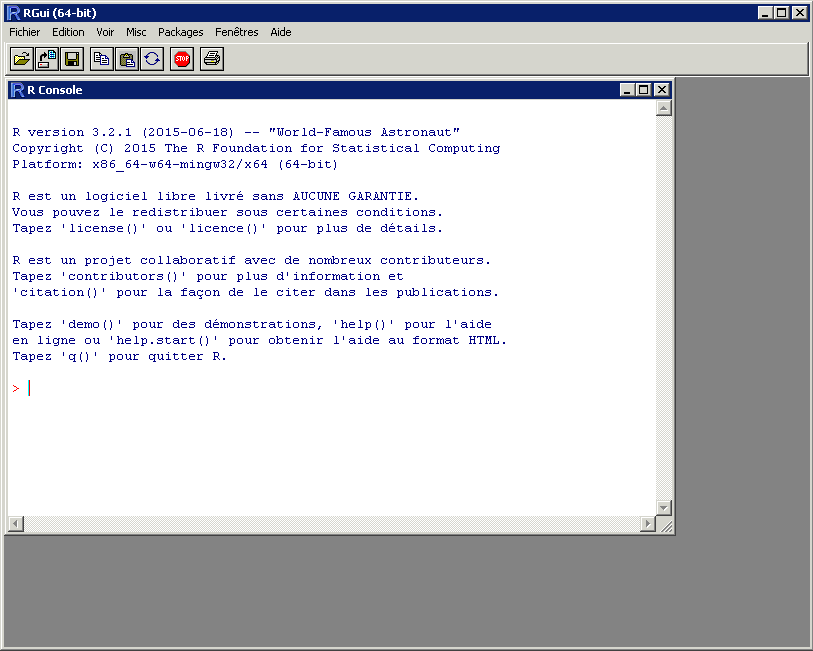
\includegraphics{../figures/Interface_R.png}
\caption{Interface fenêtrée de R sous Windows}
\end{figure}

Toutes les commandes peuvent être passées au logiciel par le biais de la
console, même si \textbf{en pratique les commandes les plus longues sont
stockées et soumises depuis un fichier de script} (\emph{cf.} la
sous-partie suivante). En particulier, il est fréquent d'effectuer dans
la console:

\begin{itemize}
\item
  \textbf{des assignations et des rappels de valeur} : le signe
  \texttt{\textless{}-} permet d'assigner des valeurs à des noms pour
  être réutilisées ultérieurement. Quand une valeur est assignée à un
  nom, il suffit de taper le nom dans la console pour afficher la
  valeur.
\item
  \textbf{des opérations sur les objets en mémoire} :

  \begin{itemize}
  \tightlist
  \item
    la fonction \texttt{ls()}\index{\texttt{ls}|textbf} affiche tous les
    objets en mémoire ;
  \item
    la fonction \texttt{str(a)}\index{\texttt{str}|textbf} affiche les
    caractéristiques (ou encore la \emph{structure}) de l'objet
    \texttt{a} (son type, sa longueur, etc.) ;
  \item
    la fonction \texttt{rm(a)}\index{\texttt{rm}|textbf} supprime
    l'objet \texttt{a}.
  \end{itemize}
\item
  \textbf{des requêtes pour l'aide} : pour afficher l'aide sur une
  fonction dont le nom est \texttt{maFonction}, il suffit d'utiliser
  \texttt{help(maFonction)}\index{\texttt{help}|textbf} ou plus
  simplement \texttt{?\ maFonction}\index{\texttt{?}|textbf}.
\item
  \textbf{des opérations simples} : le tableau ci-dessous présente
  quelques opérations arithmétiques et les symboles correspondant en R.

  \begin{longtable}[]{@{}ll@{}}
  \toprule
  Code R & Résultat\tabularnewline
  \midrule
  \endhead
  \texttt{a\ +\ b}\index{\texttt{+}|textbf} & Somme de a et
  b\tabularnewline
  \texttt{a\ -\ b}\index{\texttt{-}|textbf} & Soustraction de b à
  a\tabularnewline
  \texttt{a\ *\ b}\index{\texttt{*}|textbf} & Produit de a et
  b\tabularnewline
  \texttt{a\ /\ b}\index{\texttt{/}|textbf} & Division de a par
  b\tabularnewline
  \texttt{a\ \^{}\ b}\index{\texttt{\textasciicircum}|textbf} & a
  puissance b\tabularnewline
  \texttt{a\ \%/\%\ b}\index{\texttt{\%/\%}|textbf} & Quotient de la
  division euclidienne de a par b\tabularnewline
  \texttt{a\ \%\%\ b}\index{\texttt{\%\%}|textbf} & Reste de la division
  euclidienne de a par b\tabularnewline
  \texttt{sqrt(a)}\index{\texttt{sqrt}|textbf} & Racine carrée de
  a\tabularnewline
  \bottomrule
  \end{longtable}
\end{itemize}

~

\subsubsection{\texorpdfstring{\textbf{Cas pratique 1.1} Convertir une
durée de secondes en
minutes-secondes}{Cas pratique 1.1 Convertir une durée de secondes en minutes-secondes}}\label{cas-pratique-1.1-convertir-une-duree-de-secondes-en-minutes-secondes}

\addcontentsline{cp}{caspratique}{1.1 Convertir une durée de secondes en minutes-secondes}
Il est souvent très utile de mesurer et d'afficher la durée d'un
traitement un peu long (script exécuté régulièrement par exemple). La
fonction \texttt{system.time()}\index{\texttt{sys.time}} de R n'affiche
néanmoins que le temps écoulé en \emph{secondes}, ce qui n'est guère
lisible. \textbf{L'objectif de ce cas pratique est de convertir une
durée de secondes en minutes-secondes}.

\begin{enumerate}
\def\labelenumi{\alph{enumi}.}
\item
  Ouvrez une session AUS (en utilisant votre idep et votre mot de passe)
  et lancez le programme R (pas Rstudio).
\item
  Dans la console, associez la valeur 2456 à l'objet \texttt{duree}.
  C'est sur cette durée (en secondes) que vont porter tous les calculs.
  Une fois assignée, rappelez la valeur de \texttt{duree} dans la
  console.\index{\texttt{<-}}

  \ifsol 

  \begin{center} \rule{0.5\linewidth}{\linethickness}\end{center}

\begin{Shaded}
\begin{Highlighting}[]
\CommentTok{# Note : Pour copier-coller les éléments de solution,}
\CommentTok{# vous pouvez utiliser les raccourcis clavier Ctrl + C}
\CommentTok{# (copier) et Ctrl + V (coller).}

\CommentTok{# Pour assignez une valeur à un objet, on utilise l'opérateur <-}
\NormalTok{duree <-}\StringTok{ }\DecValTok{2456}
\CommentTok{# Pour soumettre une opération en mode console, il suffit d'appuyer}
\CommentTok{# sur ENTREE.}

\CommentTok{# Dès lors qu'une valeur est assignée à un objet, il suffit de taper}
\CommentTok{# le nom de l'objet dans la console pour rappeler sa valeur :}
\NormalTok{duree}
  \NormalTok{## [1] 2456}
\end{Highlighting}
\end{Shaded}

  \begin{center} \rule{0.5\linewidth}{\linethickness}\end{center}

  \bigskip  \fi 
\item
  Calculez le nombre de minutes correspondant à la valeur de
  \texttt{duree}. Comment obtenir un nombre entier (\emph{cf.} le
  tableau des opérations arithmétiques) ? Associez cette valeur à
  l'objet \texttt{min}.\index{\texttt{/}}\index{\texttt{\%/\%}}

  \ifsol 

  \begin{center} \rule{0.5\linewidth}{\linethickness}\end{center}

\begin{Shaded}
\begin{Highlighting}[]
\CommentTok{# Pour obtenir le nombre de minutes dans duree, il suffit de}
\CommentTok{# diviser par 60 :}
\NormalTok{duree /}\StringTok{ }\DecValTok{60}
  \NormalTok{## [1] 40.93333}
\CommentTok{# Néanmoins, pour obtenir un nombre entier de minutes, il faut utiliser}
\CommentTok{# la division euclidienne (cf. tableau)}
\NormalTok{duree %/%}\StringTok{ }\DecValTok{60}
  \NormalTok{## [1] 40}
\CommentTok{# On stocke le nombre de minutes dans l'objet min avec <-}
\NormalTok{min <-}\StringTok{ }\NormalTok{duree %/%}\StringTok{ }\DecValTok{60}
\NormalTok{min}
  \NormalTok{## [1] 40}
\end{Highlighting}
\end{Shaded}

  \begin{center} \rule{0.5\linewidth}{\linethickness}\end{center}

  \bigskip  \fi 
\item
  Calculez le nombre de secondes restantes une fois le nombre de minutes
  déterminé. Vous pouvez utiliser la flèche \(\uparrow\) du clavier pour
  rappeler et modifier le code que vous venez de soumettre. Associez
  cette valeur à l'objet \texttt{sec}.\index{\texttt{\%\%}}

  \ifsol 

  \begin{center} \rule{0.5\linewidth}{\linethickness}\end{center}

\begin{Shaded}
\begin{Highlighting}[]
\CommentTok{# Calculer le nombre de secondes restantes revient à calculer}
\CommentTok{# le reste de la division euclidienne de duree par 60 : c'est ce}
\CommentTok{# que fait l'opérateur %% (cf. tableau).}
\NormalTok{duree %%}\StringTok{ }\DecValTok{60}
  \NormalTok{## [1] 56}
\CommentTok{# A nouveau, on rappelle le code saisi précédemment avec la flèche}
\CommentTok{# HAUT du clavier et on associe la valeur à l'objet sec avec l'opérateur <-.}
\NormalTok{sec <-}\StringTok{ }\NormalTok{duree %%}\StringTok{ }\DecValTok{60}
\NormalTok{sec}
  \NormalTok{## [1] 56}
\end{Highlighting}
\end{Shaded}

  \begin{center} \rule{0.5\linewidth}{\linethickness}\end{center}

  \bigskip  \fi 
\item
  Utilisez la fonction \texttt{help()} (ou de façon équivalente
  \texttt{?}) pour recherchez de l'aide sur la fonction
  \texttt{paste()}\index{\texttt{help}}\index{\texttt{?}}\index{\texttt{paste}}.
  Que se passe-t-il quand vous soumettez le code

\begin{Shaded}
\begin{Highlighting}[]
\KeywordTok{paste}\NormalTok{(}\StringTok{"La durée est de"}\NormalTok{, duree, }\StringTok{"secondes."}\NormalTok{)}
\end{Highlighting}
\end{Shaded}

  En utilisant tous ces éléments, afficher dans la console le texte :

\begin{verbatim}
  ## [1] "Le traitement a duré `min` minutes et `sec` secondes."
\end{verbatim}

  \ifsol 

  \begin{center} \rule{0.5\linewidth}{\linethickness}\end{center}

\begin{Shaded}
\begin{Highlighting}[]
\CommentTok{# Pour consulter l'aide de R, il suffit d'utiliser la fonction help()}
\CommentTok{# avec entre parenthèses le nom de la fonction sur laquelle on souhaite}
\CommentTok{# obtenir de l'aide. }
\KeywordTok{help}\NormalTok{(paste)}
\CommentTok{# On peut aussi plus simplement utiliser ? :}
\NormalTok{? paste}
\CommentTok{# Un navigateur s'ouvre alors pour afficher la page d'aide de la fonction.}
\end{Highlighting}
\end{Shaded}

  \begin{figure}[htbp]
  \centering
  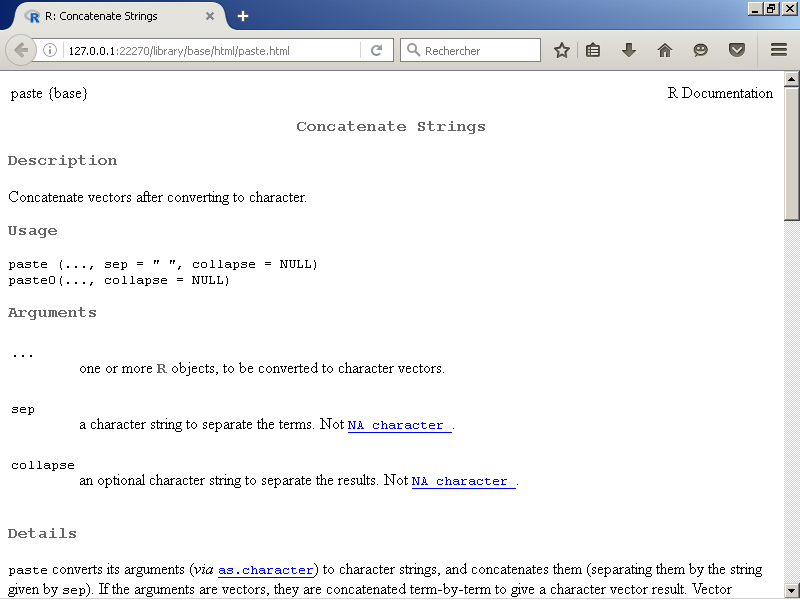
\includegraphics{../figures/Aide_paste.png}
  \caption{Aide de la fonction paste()}
  \end{figure}

\begin{Shaded}
\begin{Highlighting}[]
\CommentTok{# On y apprend que cette fonction sert à concaténer des "vecteurs"}
\CommentTok{# (cf. module 2 de la formation). En soumettant l'exemple proposé,}
\CommentTok{# on obtient :}
\KeywordTok{paste}\NormalTok{(}\StringTok{"La durée est de"}\NormalTok{, duree, }\StringTok{"secondes."}\NormalTok{)}
  \NormalTok{## [1] "La durée est de 2456 secondes."}

\CommentTok{# Ce code produit une chaîne de caractère : les chaînes de texte}
\CommentTok{# (entre "") sont reproduites telles quelles mais l'objet `duree`}
\CommentTok{# est remplacé par sa valeur. Les différents arguments de la fonction}
\CommentTok{# paste() sont séparés par des virgules.}

\CommentTok{# Pour répondre à la question, il suffit donc d'utiliser les objets}
\CommentTok{# `min` et `sec` définis précédemment comme arguments de la fonction paste() :}
\KeywordTok{paste}\NormalTok{(}\StringTok{"Le traitement a duré"}\NormalTok{, min, }\StringTok{"minutes et"}\NormalTok{, sec, }\StringTok{"secondes."}\NormalTok{)}
  \NormalTok{## [1] "Le traitement a duré 40 minutes et 56 secondes."}
\end{Highlighting}
\end{Shaded}

  \begin{center} \rule{0.5\linewidth}{\linethickness}\end{center}

  \bigskip  \fi 
\end{enumerate}

~

\subsubsection{\texorpdfstring{\textbf{Cas pratique 1.2} Manipuler des
objets en
mémoire}{Cas pratique 1.2 Manipuler des objets en mémoire}}\label{cas-pratique-1.2-manipuler-des-objets-en-memoire}

\addcontentsline{cp}{caspratique}{1.2 Manipuler des objets en mémoire}
Par défaut en mode console, l'utilisateur ne dispose d'aucune
information sur les objets stockés en mémoire. \textbf{L'objectif de ce
cas pratique est de vous familiariser avec les principales fonctions de
manipulation des objets en mémoire.}

\begin{enumerate}
\def\labelenumi{\alph{enumi}.}
\item
  Utilisez la fonction \texttt{ls()}\index{\texttt{ls}} (sans argument)
  pour afficher les objets actuellement stockés en mémoire. Affectez la
  valeur 567 à l'objet \texttt{Duree} (avec un \texttt{D} majuscule) et
  relancez la fonction \texttt{ls()}. Pourquoi R distingue-t-il les
  objets \texttt{duree} et \texttt{Duree} ?

  \ifsol 

  \begin{center} \rule{0.5\linewidth}{\linethickness}\end{center}

\begin{Shaded}
\begin{Highlighting}[]
\CommentTok{# Utilisée sans arguments, la fonction ls() liste tous les objets }
\CommentTok{# stockés dans l'environnement de référence de R}
\KeywordTok{ls}\NormalTok{()}
  \NormalTok{## [1] "duree" "min"   "sec"}
\NormalTok{Duree <-}\StringTok{ }\DecValTok{567}
\KeywordTok{ls}\NormalTok{()}
  \NormalTok{## [1] "duree" "Duree" "min"   "sec"}
\CommentTok{# R distingue les objets duree et Duree car il est sensible à la casse.}
\end{Highlighting}
\end{Shaded}

  \begin{center} \rule{0.5\linewidth}{\linethickness}\end{center}

  \bigskip  \fi 
\item
  Associez à l'objet \texttt{monTexte} la chaîne de caractère
  \texttt{"Hello\ world!"}. En utilisant la fonction
  \texttt{str()}\index{\texttt{str}}, comparez les caractéristiques des
  objets \texttt{duree} et \texttt{monTexte}. À quel type chacun de ces
  deux objets appartient-il ?

  \ifsol 

  \begin{center} \rule{0.5\linewidth}{\linethickness}\end{center}

\begin{Shaded}
\begin{Highlighting}[]
\CommentTok{# Comme dans la fonction paste(), la manipulation de chaînes }
\CommentTok{# de caractère nécessite l'utilisation de guillemets ""}
\NormalTok{monTexte <-}\StringTok{ "Hello world!"}
\KeywordTok{ls}\NormalTok{()}
  \NormalTok{## [1] "duree"    "Duree"    "min"      "monTexte" "sec"}

\CommentTok{# La fonction str(a) permet d'afficher les caractéristiques}
\CommentTok{# de l'objet a.}
\KeywordTok{str}\NormalTok{(duree)}
  \NormalTok{##  num 2456}
\KeywordTok{str}\NormalTok{(monTexte)}
  \NormalTok{##  chr "Hello world!"}
\CommentTok{# duree est un objet de type numérique alors que}
\CommentTok{# monTexte est un objet de type caractère.}
\end{Highlighting}
\end{Shaded}

  \begin{center} \rule{0.5\linewidth}{\linethickness}\end{center}

  \bigskip  \fi 
\item
  Utilisez la fonction \texttt{rm()}\index{\texttt{rm}} pour supprimer
  les objets \texttt{Duree} et \texttt{monTexte}. Vérifiez que la
  suppression est effective (et n'a pas affecté \texttt{duree}) en
  relançant la fonction \texttt{ls()}\index{\texttt{ls}}.

  \ifsol 

  \begin{center} \rule{0.5\linewidth}{\linethickness}\end{center}

\begin{Shaded}
\begin{Highlighting}[]
\CommentTok{# Objets présents au début de la question}
\KeywordTok{ls}\NormalTok{()}
  \NormalTok{## [1] "duree"    "Duree"    "min"      "monTexte" "sec"}

\CommentTok{# La fonction rm() (de l'anglais remove) permet de supprimer }
\CommentTok{# un ou plusieurs objets.}
\KeywordTok{rm}\NormalTok{(Duree, monTexte)}
\KeywordTok{ls}\NormalTok{()}
  \NormalTok{## [1] "duree" "min"   "sec"}
\CommentTok{# Les objets Duree et monTexte ont bien été supprimés.}
\end{Highlighting}
\end{Shaded}

  \begin{center} \rule{0.5\linewidth}{\linethickness}\end{center}

  \bigskip  \fi 
\item
  Recherchez de l'aide sur la fonction \texttt{rm()}\index{\texttt{rm}},
  et plus spécifiquement sur son argument \texttt{list}. En utilisant
  cet argument combiné avec la fonction
  \texttt{ls()}\index{\texttt{ls}}, écrivez une instruction qui supprime
  tous les objets dans l'environnement de référence de R.

  \ifsol 

  \begin{center} \rule{0.5\linewidth}{\linethickness}\end{center}

\begin{Shaded}
\begin{Highlighting}[]
\CommentTok{# Pour recherchez de l'aide sur une fonction, on utilise tout simplement ?}
\NormalTok{? rm}
\end{Highlighting}
\end{Shaded}

  \begin{figure}[htbp]
  \centering
  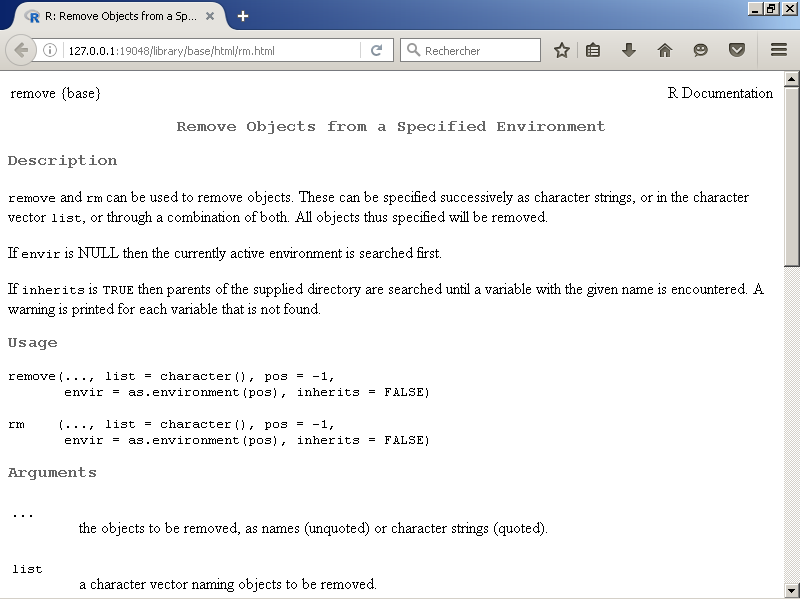
\includegraphics{../figures/Aide_rm.png}
  \caption{Aide de la fonction rm()}
  \end{figure}

\begin{Shaded}
\begin{Highlighting}[]
\CommentTok{# L'argument list permet de spécifier les objets à supprimer}
\CommentTok{# sous la forme d'une vecteur de type caractère. Or c'est précisément}
\CommentTok{# ce que produit la fonction ls() :}
\KeywordTok{ls}\NormalTok{()}
  \NormalTok{## [1] "duree" "min"   "sec"}

\CommentTok{# Pour supprimer tous les éléments en une seule commande, il suffit}
\CommentTok{# de spécifier le résultat de la commande ls() à l'argument list de la}
\CommentTok{# fonction rm() :}
\KeywordTok{rm}\NormalTok{(}\DataTypeTok{list =} \KeywordTok{ls}\NormalTok{())}

\CommentTok{# On vérifie alors qu'il n'y a plus aucun objet }
\CommentTok{# dans l'environnement de référence :}
\KeywordTok{ls}\NormalTok{()}
  \NormalTok{## character(0)}
\end{Highlighting}
\end{Shaded}

  \begin{center} \rule{0.5\linewidth}{\linethickness}\end{center}

  \bigskip  \fi 
\end{enumerate}

\subsection{Utiliser des scripts dans
RStudio}\label{utiliser-des-scripts-dans-rstudio}

Quoique toutes les fonctionnalités de R soient accessibles en mode
console, ce type d'interface présente l'inconvénient majeur de
\textbf{ne pas permettre de garder facilement une trace du code saisi}
(sinon par le biais de l'historique des commandes accessible par
\(\uparrow\)). Pour combler ce manque, les différentes interfaces
graphiques de R permettent d'utiliser des \textbf{scripts} au format
\texttt{.R}, à l'image des éditeurs de SAS (fichiers \texttt{.sas}) ou
des \emph{do-file} de Stata (fichiers \texttt{.do}).

En particulier, l'environnement de développement \textbf{RStudio}
propose de nombreuses fonctionnalités qui \textbf{rendent l'utilisation
de R beaucoup plus simple et intuitive} : explorateur d'environnements,
colorisation et auto-complétion du code, afficheur de fenêtres d'aide et
de résultats, etc.

\begin{figure}[htbp]
\centering
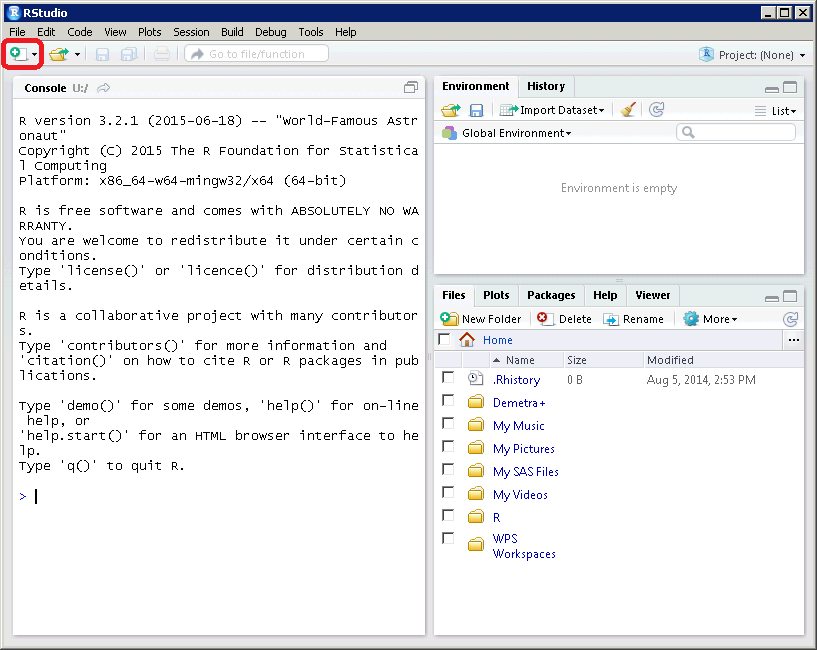
\includegraphics{../figures/Interface_RStudio_1.png}
\caption{Interface fenêtrée de \textbf{RStudio} sous Windows}
\end{figure}

À l'ouverture de \textbf{RStudio}, en règle générale trois panneaux sont
visibles :

\begin{itemize}
\tightlist
\item
  La \textbf{console} (à gauche par défaut) : la principale différence
  avec précédemment tient à la couleur du texte, noire pour les messages
  et bleue pour le signe \texttt{\textgreater{}}. Pour vider
  l'intégralité de la console, taper \texttt{Ctrl\ +\ L}.
\item
  L'\textbf{explorateur d'environnements et l'historique} (en haut à
  droite par défaut) : l'explorateur d'environnements permet d'afficher
  les objets présents (comme la fonction \texttt{ls()}) dans
  l'environnement de référence; l'historique rappelle toutes les
  commandes saisies à la manière de la touche \(\uparrow\) dans la
  console.
\item
  La \textbf{fenêtre de visualisation} (en bas à droite par défaut) : ce
  panneau intègre à la fenêtre du logiciel l'aide ou encore les
  graphiques produits.
\end{itemize}

En appuyant sur \enquote{Nouveau} \textgreater{} \enquote{Script R}
(bouton entouré en rouge dans la figure précédente), les fenêtres se
réorganisent pour faire apparaître une zone de texte : l'\textbf{éditeur
de script}.

\begin{figure}[htbp]
\centering
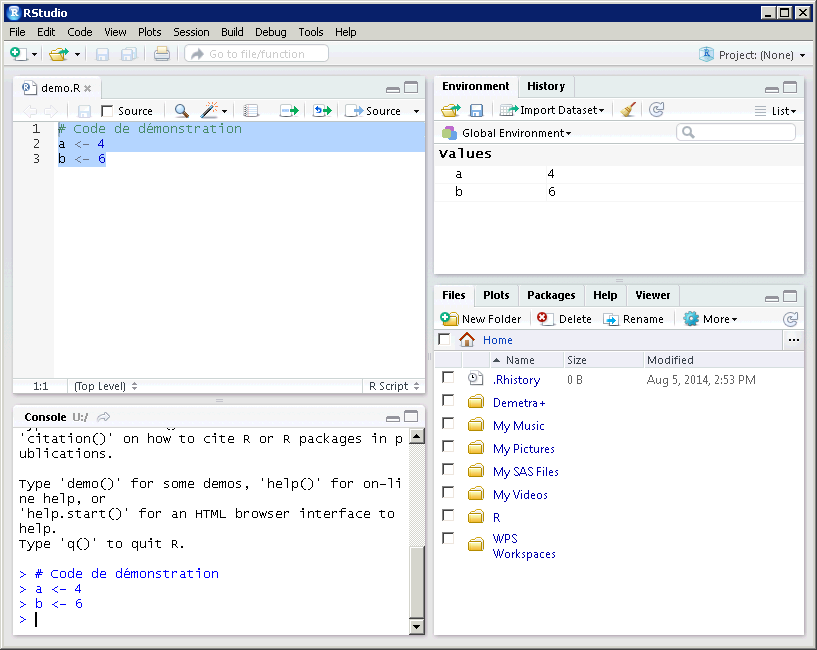
\includegraphics{../figures/Interface_RStudio_2.png}
\caption{Interface fenêtrée de \textbf{RStudio} sous Windows -- Avec
éditeur de scripts ouvert}
\end{figure}

L'utilisation de l'éditeur de scripts sous \textbf{RStudio} est analogue
à celle de l'éditeur sous SAS ou du \emph{do-file editor} de Stata :

\begin{itemize}
\tightlist
\item
  il est possible d'\textbf{enregistrer} et d'\textbf{ouvrir un script}
  avec les boutons de la barre d'outils correspondants. Le format
  d'enregistrement par défaut est \texttt{.R}, mais le fichier est
  directement lisible par n'importe quel éditeur de texte (bloc-note ou
  Notepad++ sous Windows par exemple) ;
\item
  pour \textbf{soumettre une ou plusieurs lignes de code}, il suffit de
  les sélectionner et de saisir au clavier \textbf{Ctrl~+~R} ou
  \textbf{Ctrl~+~Entrée} ;
\item
  les \textbf{éléments de syntaxe apparaissent en couleur} : les
  commentaires (précédés de \texttt{\#} à chaque ligne) en vert clair,
  les objets en noir, les nombres en bleu et les chaînes de caractère
  (entre \texttt{""} ou \texttt{\textquotesingle{}\textquotesingle{}})
  en vert foncé. Pour \textbf{commenter plusieurs lignes de code
  simultanément}, il suffit d'utiliser le raccourci
  \textbf{Ctrl~+~Maj~+~C};
\item
  des \textbf{suggestions apparaissent au cours de la frappe} : quand
  \textbf{RStudio} détecte le début du nom d'un objet déjà défini (par
  exemple une fonction), il fournit des \textbf{propositions
  d'auto-complétion}. Le logiciel double également automatiquement les
  guillemets et les parenthèses.
\end{itemize}

~

\subsubsection{\texorpdfstring{\textbf{Cas pratique 1.3} Construire une
fonction de conversion de secondes en
minutes-secondes}{Cas pratique 1.3 Construire une fonction de conversion de secondes en minutes-secondes}}\label{cas-pratique-1.3-construire-une-fonction-de-conversion-de-secondes-en-minutes-secondes}

\addcontentsline{cp}{caspratique}{1.3 Construire une fonction de conversion de secondes en minutes-secondes}
Ce cas pratique reprend les éléments du cas pratique 1.1. Son objectif
est de construire une fonction \texttt{conversion()} qui, à partir d'un
paramètre \texttt{duree} exprimé en secondes, crée une chaîne de
caractère du type

\begin{verbatim}
  ## [1] "Le traitement a duré `min` minutes et `sec` secondes."
\end{verbatim}

~

\begin{enumerate}
\def\labelenumi{\alph{enumi}.}
\item
  Toujours sur AUS, ouvrez le programme \textbf{RStudio}. Créez un
  nouveau script et sauvegardez-le sous votre répertoire personnel
  \texttt{U:\textbackslash{}} (par exemple sous
  \texttt{U:\textbackslash{}R\_initiation\textbackslash{}module1.R}).
\item
  En vous inspirant de l'exemple de la fonction \texttt{monCalcul()}
  (\emph{cf.} \emph{supra}), écrivez dans le script une première version
  de la fonction \texttt{conversion()} qui, à partir du paramètre
  \texttt{duree}, affiche le temps en secondes correspondant (sans le
  modifier dans un premier temps).\index{\texttt{function}}

  \ifsol 

  \begin{center} \rule{0.5\linewidth}{\linethickness}\end{center}

\begin{Shaded}
\begin{Highlighting}[]
\CommentTok{# La structure de base d'une définition de fonction est simple :}
\CommentTok{# l'opérateur d'assignation est utilisé pour associer à un nom}
\CommentTok{# le code de la fonction}
\NormalTok{conversion <-}\StringTok{ }\NormalTok{function(duree)\{}
  \KeywordTok{return}\NormalTok{(duree)}
\NormalTok{\}}
\CommentTok{# Dans cette première version, on ne fait que renvoyer la valeur}
\CommentTok{# de duree à l'identique.}
\KeywordTok{conversion}\NormalTok{(}\DecValTok{2456}\NormalTok{)}
  \NormalTok{## [1] 2456}
\end{Highlighting}
\end{Shaded}

  \begin{center} \rule{0.5\linewidth}{\linethickness}\end{center}

  \bigskip  \fi 
\item
  Intégrez à la fonction \texttt{conversion()} les éléments définis aux
  différentes étapes du cas pratique 1.1 (définition de \texttt{min}, de
  \texttt{sec}, concaténation avec la fonction \texttt{paste()}) pour
  atteindre le résultat désiré. Testez votre fonction avec les valeurs
  2456 et 7564.\index{\texttt{function}}

  \ifsol 

  \begin{center} \rule{0.5\linewidth}{\linethickness}\end{center}

\begin{Shaded}
\begin{Highlighting}[]
\CommentTok{# On reprend les éléments du cas pratique 1.1 pour rendre la fonction}
\CommentTok{# véritablement opérante :}
\NormalTok{conversion <-}\StringTok{ }\NormalTok{function(duree)\{}
  \NormalTok{min <-}\StringTok{ }\NormalTok{duree %/%}\StringTok{ }\DecValTok{60}
  \NormalTok{sec <-}\StringTok{ }\NormalTok{duree %%}\StringTok{ }\DecValTok{60}
  \NormalTok{resultat <-}\StringTok{ }\KeywordTok{paste}\NormalTok{(}
    \StringTok{"Le traitement a duré"}\NormalTok{, min, }\StringTok{"minutes et"}\NormalTok{, sec, }\StringTok{"secondes."}
  \NormalTok{)}
  \KeywordTok{return}\NormalTok{(resultat)}
\NormalTok{\}}
\KeywordTok{conversion}\NormalTok{(}\DecValTok{2456}\NormalTok{)}
  \NormalTok{## [1] "Le traitement a duré 40 minutes et 56 secondes."}
\KeywordTok{conversion}\NormalTok{(}\DecValTok{7564}\NormalTok{)}
  \NormalTok{## [1] "Le traitement a duré 126 minutes et 4 secondes."}
\end{Highlighting}
\end{Shaded}

  \begin{center} \rule{0.5\linewidth}{\linethickness}\end{center}

  \bigskip  \fi 
\item
  Observez comment l'éditeur colorise votre code, mais aussi les
  différents objets créés dans l'explorateur d'environnements. Saisissez
  dans l'éditeur ou la console les lettres \texttt{conver} et utilisez
  l'auto-complétion pour sélectionner votre fonction. Ajoutez des
  commentaires (précédés par \texttt{\#}), manuellement ou en utilisant
  le raccourci clavier Ctrl~+~Maj~+~C.
\end{enumerate}

~

\section{Charger et explorer des
données}\label{charger-et-explorer-des-donnees}

\textbf{Explorer des données statistiques avec R est relativement
intuitif}, en particulier grâce aux fonctionnalités de RStudio :
affichage des objets chargés en mémoire, explorateur d'objets,
auto-complétion. \textbf{Manipuler des données exige en revanche une
plus grande maîtrise des briques élémentaires du langage} qui sont
présentées en détails dans le module 2 de la formation.

~

R travaille sur des \textbf{objets stockés en mémoire} : pour explorer
des données, la première étape consiste donc à les \textbf{charger en
mémoire depuis leur emplacement sur le disque dur de l'ordinateur}. On
utilise en général pour ce faire la \textbf{fonction
\texttt{load()}}\index{\texttt{load}|textbf}:

\begin{Shaded}
\begin{Highlighting}[]
\CommentTok{# Chargement des données du fichier module1.RData}
\KeywordTok{load}\NormalTok{(}\StringTok{"U:/R_initiation/donnees/module1.RData"}\NormalTok{)}
\CommentTok{# NOTE : DANS R LES CHEMINS SONT INDIQUES AVEC DES / ET NON DES \textbackslash{}}
\end{Highlighting}
\end{Shaded}

\textbf{La fonction \texttt{load()} charge dans l'environnement de
référence les objets contenus dans le fichier \texttt{module1.RData}} en
les décompressant au passage (par défaut les fichiers saugevardés par R
sont compressés). L'environnement de référence comporte désormais deux
nouveaux objets :

\begin{Shaded}
\begin{Highlighting}[]
\CommentTok{# Fichiers présents dans l'environnement de référence}
\KeywordTok{ls}\NormalTok{()}
  \NormalTok{## [1] "bpe"        "conversion" "rp"}

\CommentTok{# Caractéristiques de l'objet bpe}
\KeywordTok{str}\NormalTok{(bpe)}
  \NormalTok{## 'data.frame':  358 obs. of  8 variables:}
  \NormalTok{##  $ ancreg  : chr  "11" "11" "11" "11" ...}
  \NormalTok{##  $ reg     : chr  "11" "11" "11" "11" ...}
  \NormalTok{##  $ dep     : chr  "92" "92" "92" "92" ...}
  \NormalTok{##  $ depcom  : chr  "92046" "92046" "92046" "92046" ...}
  \NormalTok{##  $ dciris  : chr  "92046_0000" "92046_0000" "92046_0000" "92046_0000" ...}
  \NormalTok{##  $ an      : chr  "2015" "2015" "2015" "2015" ...}
  \NormalTok{##  $ typequ  : chr  "D104" "D109" "F102" "F107" ...}
  \NormalTok{##  $ nb_equip: num  1 1 2 1 2 1 2 1 1 1 ...}
\end{Highlighting}
\end{Shaded}

\textbf{L'objet \texttt{bpe} correspond à une extraction de la
\href{https://www.insee.fr/fr/statistiques/2410933}{Base permanente des
équipements 2015} restreinte aux équipements de la ville de Malakoff
(code Insee 92046)}. La nomenclature des équipements est présentée sur
\href{https://www.insee.fr/fr/statistiques/2578377}{cette page}.

Pour parcourir ce fichier dans \textbf{RStudio}, il suffit de
\textbf{cliquer sur son nom dans l'explorateur d'environnements}.
Plusieurs manipulations peuvent par ailleurs être effectuées de façon
relativement intuitive:

~

\begin{itemize}
\item
  \textbf{afficher les premières lignes} avec la fonction
  \texttt{head()}, les \textbf{dernières lignes} avec la fonction
  \texttt{tail()}\index{\texttt{head}}\index{\texttt{tail}} :

\begin{Shaded}
\begin{Highlighting}[]
\CommentTok{# Affichage des premières et dernières lignes de l'objet bpe}
\KeywordTok{head}\NormalTok{(bpe)}
  \NormalTok{##   ancreg reg dep depcom     dciris   an typequ nb_equip}
  \NormalTok{## 1     11  11  92  92046 92046_0000 2015   D104        1}
  \NormalTok{## 2     11  11  92  92046 92046_0000 2015   D109        1}
  \NormalTok{## 3     11  11  92  92046 92046_0000 2015   F102        2}
  \NormalTok{## 4     11  11  92  92046 92046_0000 2015   F107        1}
  \NormalTok{## 5     11  11  92  92046 92046_0000 2015   F111        2}
  \NormalTok{## 6     11  11  92  92046 92046_0000 2015   F112        1}
\KeywordTok{tail}\NormalTok{(bpe)}
  \NormalTok{##     ancreg reg dep depcom     dciris   an typequ nb_equip}
  \NormalTok{## 353     11  11  92  92046 92046_0111 2015   D233        1}
  \NormalTok{## 354     11  11  92  92046 92046_0111 2015   D235        1}
  \NormalTok{## 355     11  11  92  92046 92046_0111 2015   D301        1}
  \NormalTok{## 356     11  11  92  92046 92046_0111 2015   D501        2}
  \NormalTok{## 357     11  11  92  92046 92046_0111 2015   E101        5}
  \NormalTok{## 358     11  11  92  92046 92046_0111 2015   F121        1}
\end{Highlighting}
\end{Shaded}
\end{itemize}

~

\begin{itemize}
\item
  \textbf{accéder au contenu d'une variable avec l'opérateur
  \texttt{\$}}\index{\texttt{\$}} (ici uniquement les 20 premières
  valeurs pour des raisons de présentation) :

\begin{Shaded}
\begin{Highlighting}[]
\CommentTok{# Affichage des premières de la variable codant le type d'équipement}
\NormalTok{bpe$typequ}
\end{Highlighting}
\end{Shaded}

\begin{verbatim}
  ##  [1] "D104" "D109" "F102" "F107" "F111" "F112" "F113" "F120"
  ##  [9] "F121" "F303" "A301" "A401" "A402" "A403" "A404" "A504"
  ## [17] "A507" "B101" "B304" "B306"
\end{verbatim}
\end{itemize}

~

\begin{itemize}
\item
  \textbf{calculer le total et des statistiques descriptives} sur une
  variable de nature quantitative avec les fonctions
  \texttt{sum()}\index{\texttt{sum}} et
  \texttt{summary()}\index{\texttt{summary}} :

\begin{Shaded}
\begin{Highlighting}[]
\CommentTok{# Total et distribution de la variable dénombrant le nombre d'équipements}
\CommentTok{# par iris et par type}
\KeywordTok{sum}\NormalTok{(bpe$nb_equip)}
  \NormalTok{## [1] 867}
\KeywordTok{summary}\NormalTok{(bpe$nb_equip)}
  \NormalTok{##    Min. 1st Qu.  Median    Mean 3rd Qu.    Max. }
  \NormalTok{##   1.000   1.000   1.000   2.422   3.000  33.000}
\end{Highlighting}
\end{Shaded}
\end{itemize}

~

\begin{itemize}
\item
  \textbf{déterminer les modalités distinctes et tabuler} une variable
  de nature qualitative avec les fonctions
  \texttt{unique()}\index{\texttt{unique}} et
  \texttt{table()}\index{\texttt{table}} :

\begin{Shaded}
\begin{Highlighting}[]
\CommentTok{# Liste des iris associés à la commune de Malakoff}
\KeywordTok{unique}\NormalTok{(bpe$dciris)}
  \NormalTok{##  [1] "92046_0000" "92046_0101" "92046_0102" "92046_0103"}
  \NormalTok{##  [5] "92046_0104" "92046_0105" "92046_0106" "92046_0107"}
  \NormalTok{##  [9] "92046_0108" "92046_0109" "92046_0110" "92046_0111"}

\CommentTok{# Nombre de types d'équipements distincts par iris à Malakoff}
\KeywordTok{table}\NormalTok{(bpe$dciris)}
  \NormalTok{## }
  \NormalTok{## 92046_0000 92046_0101 92046_0102 92046_0103 92046_0104 }
  \NormalTok{##         10         20         46         35         27 }
  \NormalTok{## 92046_0105 92046_0106 92046_0107 92046_0108 92046_0109 }
  \NormalTok{##         61         35         37         29          9 }
  \NormalTok{## 92046_0110 92046_0111 }
  \NormalTok{##         29         20}
\end{Highlighting}
\end{Shaded}
\end{itemize}

~

\begin{itemize}
\item
  \textbf{appliquer une fonction selon les modalités d'une autre
  variable} avec la fonction \texttt{by()}\index{\texttt{by}} :

\begin{Shaded}
\begin{Highlighting}[]
\CommentTok{# Nombre total d'équipements par iris}
\KeywordTok{by}\NormalTok{(bpe$nb_equip, bpe$dciris, sum)}
  \NormalTok{## bpe$dciris: 92046_0000}
  \NormalTok{## [1] 13}
  \NormalTok{## ------------------------------------------------ }
  \NormalTok{## bpe$dciris: 92046_0101}
  \NormalTok{## [1] 40}
  \NormalTok{## ------------------------------------------------ }
  \NormalTok{## bpe$dciris: 92046_0102}
  \NormalTok{## [1] 134}
  \NormalTok{## ------------------------------------------------ }
  \NormalTok{## bpe$dciris: 92046_0103}
  \NormalTok{## [1] 129}
  \NormalTok{## ------------------------------------------------ }
  \NormalTok{## bpe$dciris: 92046_0104}
  \NormalTok{## [1] 52}
  \NormalTok{## ------------------------------------------------ }
  \NormalTok{## bpe$dciris: 92046_0105}
  \NormalTok{## [1] 187}
  \NormalTok{## ------------------------------------------------ }
  \NormalTok{## bpe$dciris: 92046_0106}
  \NormalTok{## [1] 60}
  \NormalTok{## ------------------------------------------------ }
  \NormalTok{## bpe$dciris: 92046_0107}
  \NormalTok{## [1] 71}
  \NormalTok{## ------------------------------------------------ }
  \NormalTok{## bpe$dciris: 92046_0108}
  \NormalTok{## [1] 60}
  \NormalTok{## ------------------------------------------------ }
  \NormalTok{## bpe$dciris: 92046_0109}
  \NormalTok{## [1] 9}
  \NormalTok{## ------------------------------------------------ }
  \NormalTok{## bpe$dciris: 92046_0110}
  \NormalTok{## [1] 64}
  \NormalTok{## ------------------------------------------------ }
  \NormalTok{## bpe$dciris: 92046_0111}
  \NormalTok{## [1] 48}
\end{Highlighting}
\end{Shaded}
\end{itemize}

~

\begin{itemize}
\item
  \textbf{faire des représentation graphiques simples} avec les
  fonctions \texttt{pie()}\index{\texttt{pie}},
  \texttt{barplot()}\index{\texttt{barplot}} et
  \texttt{plot()}\index{\texttt{plot}} :

\begin{Shaded}
\begin{Highlighting}[]
\CommentTok{# Représentation du nombre total d'équipements par iris}
\KeywordTok{pie}\NormalTok{(}
  \KeywordTok{by}\NormalTok{(bpe$nb_equip,bpe$dciris,sum)}
  \NormalTok{, }\DataTypeTok{main =} \StringTok{"Nombre d'équipements par iris}\CharTok{\textbackslash{}n}\StringTok{de la ville de Malakoff"}
\NormalTok{)}
\end{Highlighting}
\end{Shaded}

  \begin{center}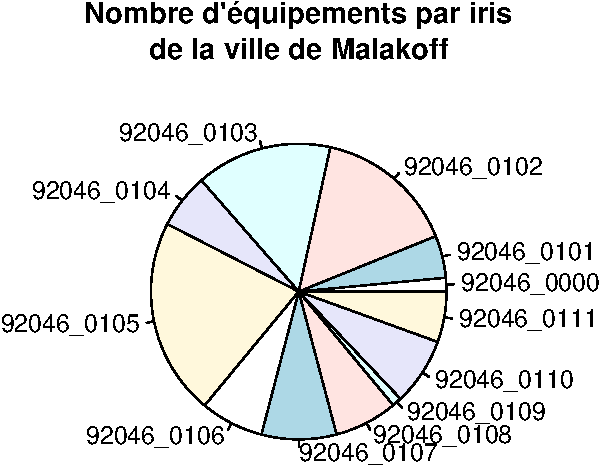
\includegraphics{livret_files/figure-latex/bpe_pie-1} \end{center}
\end{itemize}

\begin{center}\rule{0.5\linewidth}{\linethickness}\end{center}

\textbf{Remarque} D'un point de vue technique, \textbf{l'objet
\texttt{bpe} est de type \texttt{data.frame}}, qui correspond au format
le plus fréquent pour les tableaux de données dans R. Ce type d'objet
est \textbf{relativement complexe et est présenté en détails dans le
module 3 de la formation}.

\begin{center}\rule{0.5\linewidth}{\linethickness}\end{center}

~

\subsubsection{\texorpdfstring{\textbf{Cas pratique 1.4} Charger et
explorer des données : Le recensement de la population 2013 dans les
Hauts-de-Seine}{Cas pratique 1.4 Charger et explorer des données : Le recensement de la population 2013 dans les Hauts-de-Seine}}\label{cas-pratique-1.4-charger-et-explorer-des-donnees-le-recensement-de-la-population-2013-dans-les-hauts-de-seine}

\addcontentsline{cp}{caspratique}{1.4 Charger et explorer des données : Le recensement de la population 2013 dans les Hauts-de-Seine}
Ce cas pratique vise à charger et à effectuer \textbf{quelques
manipulations simples sur une extraction du fichier du recensement de la
population (RP) 2013 dans les Hauts-de-Seine} (accessible sur le
\href{https://www.insee.fr/fr/statistiques/2409491}{site de l'Insee}).
Les données ont été préalablement téléchargées et converties (\emph{cf.}
sous-partie suivante) et sont contenues dans le fichier
\texttt{module1.RData}.

\begin{enumerate}
\def\labelenumi{\alph{enumi}.}
\item
  L'ensemble des données de la formation sont contenues dans le fichier
  \href{http://r.slmc.fr/donnees.zip}{donnees.zip}. Téléchargez ce
  fichier, copiez-collez puis décompressez-le sous AUS dans le
  répertoire
  \texttt{U:\textbackslash{}R\_initiation\textbackslash{}donnees}.
\item
  Utilisez la fonction \texttt{load()}\index{\texttt{load}} pour charger
  les données contenues dans le fichier
  \texttt{U:\textbackslash{}R\_initiation\textbackslash{}donnees\textbackslash{}module1.RData}.
  \textbf{Pensez à bien utiliser des \texttt{/} et non des
  \texttt{\textbackslash{}} dans le chemin du fichier} (sans quoi le
  chargement ne fonctionnera pas). Affichez les caractéristiques de
  l'objet \texttt{rp} : combien ce fichier comporte-t-il d'observations
  et de variables ? Affichez ses premières lignes.\index{\texttt{head}}

  \ifsol 

  \begin{center} \rule{0.5\linewidth}{\linethickness}\end{center}

\begin{Shaded}
\begin{Highlighting}[]
\CommentTok{# Chargement du fichier exemples.RData}
\KeywordTok{load}\NormalTok{(}\StringTok{"U:/R_initiation/donnees/module1.RData"}\NormalTok{)}
\CommentTok{# NOTE : DANS R LES CHEMINS SONT INDIQUES AVEC DES / ET NON DES \textbackslash{}}
\end{Highlighting}
\end{Shaded}

\begin{Shaded}
\begin{Highlighting}[]
\CommentTok{# Objets présents dans l'environnement de travail}
\KeywordTok{ls}\NormalTok{()}
  \NormalTok{## [1] "bpe"        "conversion" "rp"}

\CommentTok{# Caractéristiques de l'objet rp}
\KeywordTok{str}\NormalTok{(rp)}
  \NormalTok{## 'data.frame':  609446 obs. of  6 variables:}
  \NormalTok{##  $ DEPT  : int  92 92 92 92 92 92 92 92 92 92 ...}
  \NormalTok{##  $ IPONDI: num  3.49 3.49 3.49 1.1 1.1 ...}
  \NormalTok{##  $ ANAI  : int  1960 1938 1936 2008 2004 1972 1951 1978 1976 1993 ...}
  \NormalTok{##  $ SEXE  : int  1 2 1 2 2 2 1 2 1 2 ...}
  \NormalTok{##  $ STOCD : chr  "10" "10" "10" "10" ...}
  \NormalTok{##  $ CS1   : int  8 7 7 8 8 8 3 3 3 8 ...}
\CommentTok{# Le fichier rp comporte 609 446 observations et 6 variables}

\CommentTok{# Pour afficher les premières lignes d'une table, on utilise}
\CommentTok{# la fonction head()}
\KeywordTok{head}\NormalTok{(rp)}
  \NormalTok{##   DEPT   IPONDI ANAI SEXE STOCD CS1}
  \NormalTok{## 1   92 3.492757 1960    1    10   8}
  \NormalTok{## 2   92 3.492757 1938    2    10   7}
  \NormalTok{## 3   92 3.492757 1936    1    10   7}
  \NormalTok{## 4   92 1.101669 2008    2    10   8}
  \NormalTok{## 5   92 1.101669 2004    2    10   8}
  \NormalTok{## 6   92 1.101669 1972    2    10   8}
\end{Highlighting}
\end{Shaded}

  \begin{center} \rule{0.5\linewidth}{\linethickness}\end{center}

  \bigskip  \fi 
\item
  Utilisez l'opérateur \texttt{\$}\index{\texttt{\$}} pour afficher les
  valeurs de la variable de pondération \texttt{IPONDI}. Pensez à bien
  respecter la casse du nom de la variable. Appliquez la fonction
  \texttt{sum()}\index{\texttt{sum}} à la variable \texttt{IPONDI} pour
  déterminer la population totale des Hauts-de-Seine au sens du RP 2013
  (\emph{i.e.} calculer la somme de la variable \texttt{IPONDI}).

  \ifsol 

  \begin{center} \rule{0.5\linewidth}{\linethickness}\end{center}

\begin{Shaded}
\begin{Highlighting}[]
\CommentTok{# Affichage du contenu de la variable IPONDI}
\NormalTok{rp$IPONDI}
\CommentTok{# Note : pour des raisons de présentation, seules les 20 premières valeurs}
\CommentTok{# sont affichées ici.}
\end{Highlighting}
\end{Shaded}

\begin{verbatim}
  ##  [1] 3.4927574 3.4927574 3.4927574 1.1016688 1.1016688 1.1016688
  ##  [7] 1.1016688 3.6388523 3.6388523 0.8573350 0.8573350 3.7741295
  ## [13] 3.7741295 3.5340019 1.0162282 1.0343014 1.0343014 0.8821233
  ## [19] 0.8821233 3.3128186
\end{verbatim}

\begin{Shaded}
\begin{Highlighting}[]
\KeywordTok{sum}\NormalTok{(rp$IPONDI)}
  \NormalTok{## [1] 1591365}
\CommentTok{# La population des Hauts-de-Seine au sens du RP 2013 est de}
\CommentTok{# 1 591 365 habitants.}
\end{Highlighting}
\end{Shaded}

  \begin{center} \rule{0.5\linewidth}{\linethickness}\end{center}

  \bigskip  \fi 
\item
  Affichez les modalités distinctes de la variable
  \texttt{SEXE}\index{\texttt{unique}}. Appliquez la fonction
  \texttt{table()}\index{\texttt{table}} à cette variable pour
  déterminer la répartition par sexe des individus recensés. Combinez
  les fonctions \texttt{by()}\index{\texttt{by}} et
  \texttt{sum()}\index{\texttt{sum}} pour calculer la somme de la
  variable \texttt{IPONDI} selon les modalités de la variable
  \texttt{SEXE}.

  \ifsol 

  \begin{center} \rule{0.5\linewidth}{\linethickness}\end{center}

\begin{Shaded}
\begin{Highlighting}[]
\CommentTok{# Pour afficher les modalités distinctes d'une variable, on utilise}
\CommentTok{# la fonction unique()}
\KeywordTok{unique}\NormalTok{(rp$SEXE)}
  \NormalTok{## [1] 1 2}
\CommentTok{# Comme souvent, le sexe est codé par un chiffre, "1" pour}
\CommentTok{# les hommes et "2" pour les femmes.}
\KeywordTok{table}\NormalTok{(rp$SEXE)}
  \NormalTok{## }
  \NormalTok{##      1      2 }
  \NormalTok{## 290444 319002}
\CommentTok{# La fonction table() permet d'effectuer une tabulation}
\CommentTok{# simple (et non pondérée) d'une variable}

\CommentTok{# Pour obtenir la somme des poids par sexe, on peut recourir}
\CommentTok{# à la fonction by() combinée à la fonction sum()}
\KeywordTok{by}\NormalTok{(rp$IPONDI, rp$SEXE, sum)}
  \NormalTok{## rp$SEXE: 1}
  \NormalTok{## [1] 758656.9}
  \NormalTok{## ------------------------------------------------ }
  \NormalTok{## rp$SEXE: 2}
  \NormalTok{## [1] 832707.8}
\CommentTok{# Au RP 2013, le département des Hauts-de-Seine comptait 758 657 hommes}
\CommentTok{# et 832 708 femmes.}
\end{Highlighting}
\end{Shaded}

  \begin{center} \rule{0.5\linewidth}{\linethickness}\end{center}

  \bigskip  \fi 
\item
  (Optionnel) Utilisez les résultats des deux questions précédentes pour
  calculer le pourcentage d'hommes et de femmes dans les Hauts-de-Seine
  au sens du RP 2013. Représentez ces données avec un diagramme
  circulaire.\index{\texttt{by}}\index{\texttt{pie}}

  \ifsol 

  \begin{center} \rule{0.5\linewidth}{\linethickness}\end{center}

\begin{Shaded}
\begin{Highlighting}[]
\CommentTok{# Plusieurs méthodes existent pour calculer un pourcentage}
\CommentTok{# à partir d'un objet de table(). La plus simple est}
\CommentTok{# de diviser par la taille totale de la population}
\CommentTok{# calculée à la question b.}
\KeywordTok{by}\NormalTok{(rp$IPONDI, rp$SEXE, sum)/}\KeywordTok{sum}\NormalTok{(rp$IPONDI)}
  \NormalTok{## rp$SEXE: 1}
  \NormalTok{## [1] 0.4767335}
  \NormalTok{## ------------------------------------------------ }
  \NormalTok{## rp$SEXE: 2}
  \NormalTok{## [1] 0.5232665}

\CommentTok{# Pour représenter ces données avec un diagramme}
\CommentTok{# circulaire, on utilise la fonction pie()}
\KeywordTok{pie}\NormalTok{(}
  \KeywordTok{by}\NormalTok{(rp$IPONDI, rp$SEXE, sum)/}\KeywordTok{sum}\NormalTok{(rp$IPONDI)}
  \NormalTok{, }\DataTypeTok{main =} \StringTok{"Hommes et femmes dans les Hauts-de-Seine}\CharTok{\textbackslash{}n}\StringTok{au RP 2013"}
\NormalTok{)}
\end{Highlighting}
\end{Shaded}

  \begin{center}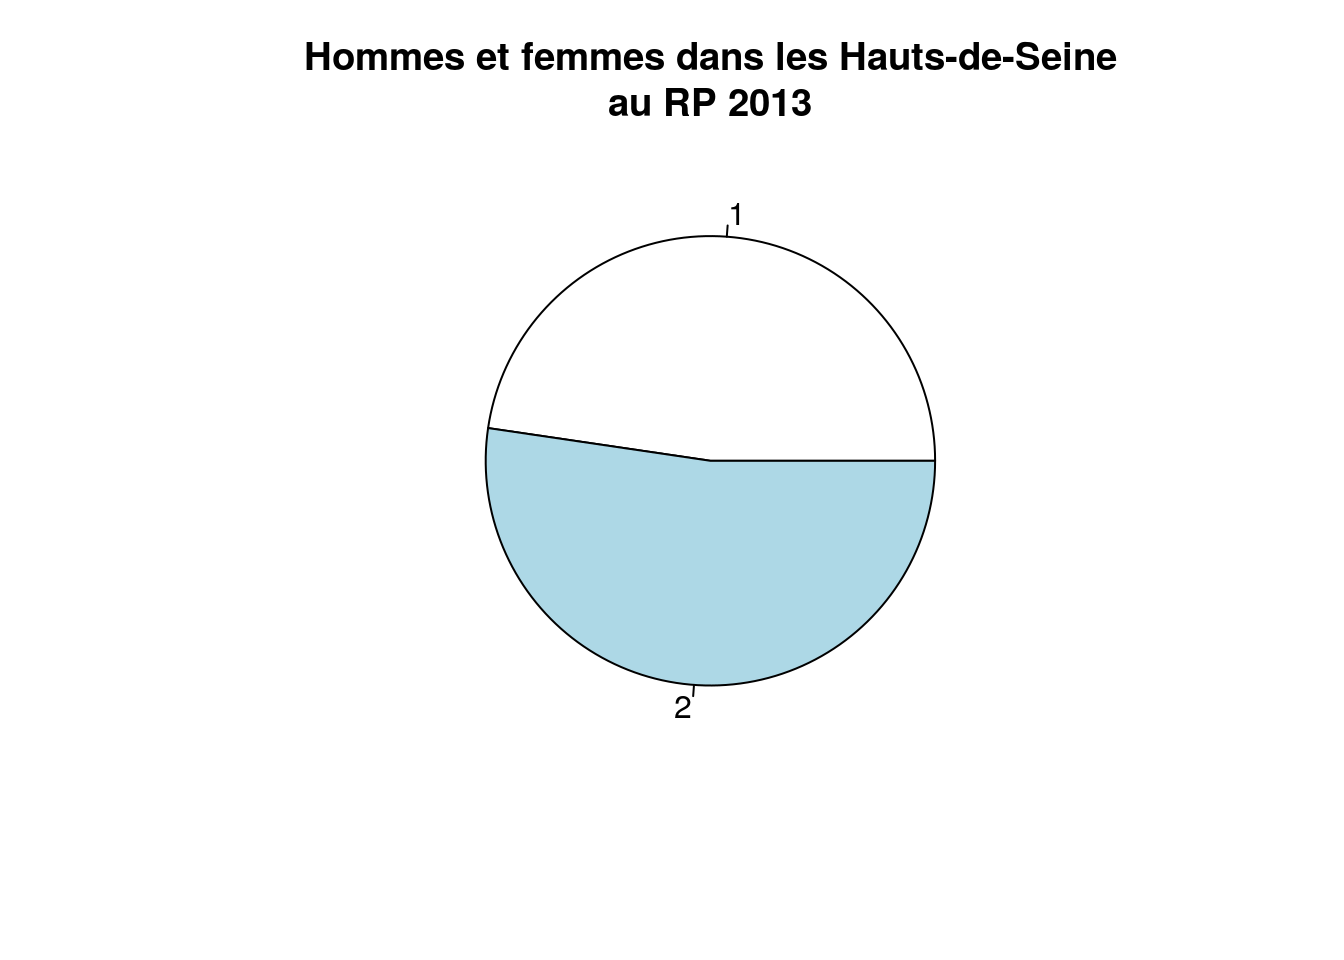
\includegraphics{livret_files/figure-latex/rp_pie-1} \end{center}

  \begin{center} \rule{0.5\linewidth}{\linethickness}\end{center}

  \bigskip  \fi 
\end{enumerate}

\section{\texorpdfstring{Importer des données à l'aide de
\emph{packages}}{Importer des données à l'aide de packages}}\label{importer-des-donnees-a-laide-de-packages}

En règle générale, les fichiers de données sur lesquels on souhaite
travailler ne sont pas en format R natif : il convient donc de les
\textbf{importer}. \textbf{R dispose de très nombreuses fonctions pour
importer des données provenant d'autres logiciels} : SAS, Stata, Excel,
etc. Toutes ne sont cependant pas chargées par défaut au démarrage du
logiciel, mais sont facilement accessibles par le biais de
\emph{packages}.

Le \enquote{fil rouge} de cette sous-partie est l'\textbf{importation
d'autres données de la Base permanente des équipements} (relatives à
Montrouge, code Insee 92049) \textbf{et stockées dans différents
formats} (\texttt{bpe2.csv}, \texttt{bpe2.dbf}, \texttt{bpe2.sas7bdat}).
\textbf{L'utilisation des \emph{packages}, leur chargement et leur
installation sont présentés en parallèle}.

\textbf{Pour faciliter l'import de fichiers différents, on modifie le
répertoire de travail} (\emph{working directory}) \textbf{de R} : il
s'agit du répertoire dans lequel le logiciel \textbf{recherche par
défaut les fichiers à importer}. Une fois le répertoire de travail
convenablement défini (avec la fonction
\texttt{setwd()}\index{\texttt{setwd}}), il suffit de saisir le nom du
fichier à importer pour que R le trouve automatiquement
\index{\texttt{load}}:

\begin{Shaded}
\begin{Highlighting}[]
\CommentTok{# Définition du répertoire de la formation comme répertoire de travail}
\KeywordTok{setwd}\NormalTok{(}\StringTok{"U:/R_initiation/donnees"}\NormalTok{)}

\CommentTok{# Utilisation de la fonction load() sans avoir à indiquer un chemin}
\KeywordTok{load}\NormalTok{(}\StringTok{"module1.RData"}\NormalTok{)}
\end{Highlighting}
\end{Shaded}

\subsection{\texorpdfstring{Importer des fichiers plats avec
\texttt{read.table()}}{Importer des fichiers plats avec read.table()}}\label{importer-des-fichiers-plats-avec-read.table}

R dispose nativement d'un fonction capable de lire les fichiers dits
\enquote{plats} (\texttt{.txt}, \texttt{.csv} ou \texttt{.dlm} le plus
souvent) : la \textbf{fonction
\texttt{read.table()}}\index{\texttt{read.table}|textbf} (taper
\texttt{?\ read.table} pour afficher sa page d'aide). Cette fonction
comporte un grand nombre de paramètres susceptibles d'être ajustés au
format du fichier en entrée : délimiteur, séparateur de décimales, etc.

Afin de faciliter l'utilisation de cette fonction, des fonctions
\enquote{alias} sont également disponibles qui correspondent à des
\textbf{versions pré-paramétrées de \texttt{read.table()}}. En
particulier :

\begin{itemize}
\tightlist
\item
  \texttt{read.csv()}\index{\texttt{read.csv}|textbf} importe des
  fichiers dont les colonnes sont \textbf{séparées par des virgules} ;
\item
  \texttt{read.delim()}\index{\texttt{read.delim}|textbf} importe des
  fichiers dont les colonnes sont \textbf{séparées par des tabulations}.
\end{itemize}

Les colonnes du fichier \texttt{bpe2.csv} utilisé dans cet exemple sont
\textbf{séparées par des virgules} (comme ceux des fichiers produits par
défaut par LibreOffice Calc) : c'est donc la fonction
\texttt{read.csv()} qu'il convient d'utiliser :

\begin{Shaded}
\begin{Highlighting}[]
\CommentTok{# Chargement du fichier bpe2.csv}
\NormalTok{bpe2_csv <-}\StringTok{ }\KeywordTok{read.csv}\NormalTok{(}\StringTok{"bpe2.csv"}\NormalTok{)}

\CommentTok{# Premières lignes de bpe2_csv}
\KeywordTok{head}\NormalTok{(bpe2_csv)}
  \NormalTok{##   ancreg reg dep depcom     dciris   an typequ nb_equip}
  \NormalTok{## 1     11  11  92  92049 92049_0000 2015   B301        1}
  \NormalTok{## 2     11  11  92  92049 92049_0000 2015   F101        1}
  \NormalTok{## 3     11  11  92  92049 92049_0000 2015   F112        2}
  \NormalTok{## 4     11  11  92  92049 92049_0000 2015   F114        1}
  \NormalTok{## 5     11  11  92  92049 92049_0000 2015   F120        1}
  \NormalTok{## 6     11  11  92  92049 92049_0000 2015   F121        4}
\end{Highlighting}
\end{Shaded}

\subsection{\texorpdfstring{Importer des fichiers \texttt{.dbf} ou
\texttt{.dta} avec le \emph{package}
\texttt{foreign}}{Importer des fichiers .dbf ou .dta avec le package foreign}}\label{importer-des-fichiers-.dbf-ou-.dta-avec-le-package-foreign}

Au-delà des fonctions natives de R, plusieurs \emph{packages} permettent
d'importer facilement des données dans R, dont le \emph{package}
\texttt{foreign}. Dans \textbf{RStudio}, la sous-fenêtre \emph{Packages}
de la fenêtre de visualisation (en bas à droite par défaut) permet
d'afficher l'ensemble des \emph{packages} installés avec une description
succincte.

\begin{figure}[htbp]
\centering
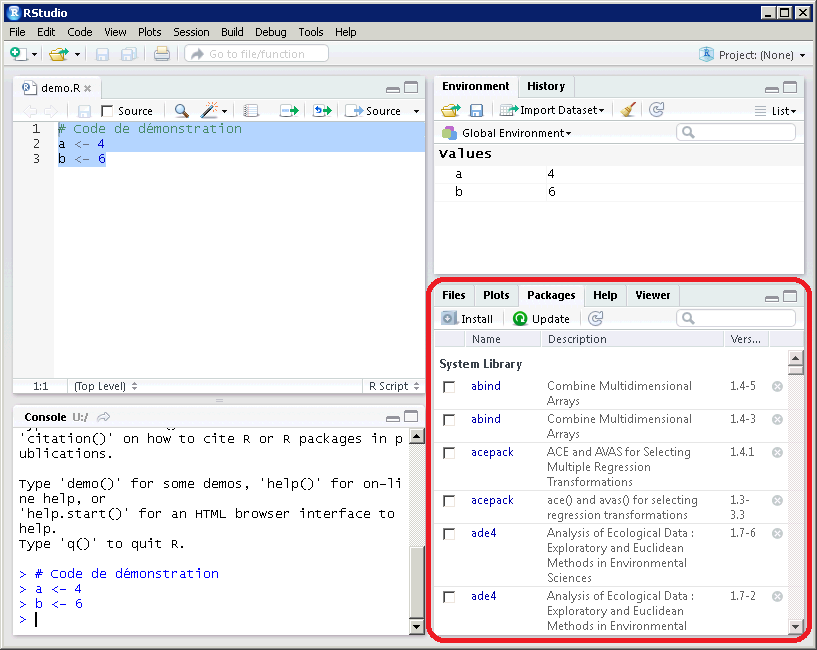
\includegraphics{../figures/Interface_RStudio_3.png}
\caption{Interface fenêtrée de \textbf{RStudio} sous Windows -- Liste
des \emph{packages} installés}
\end{figure}

Le \emph{package} \texttt{foreign} a la particularité d'être
\textbf{pré-installé} : pour utiliser ses fonctions, il suffit de le
charger avec la fonction \texttt{library()} (une fois par session
suffit).

\begin{Shaded}
\begin{Highlighting}[]
\CommentTok{# Chargement du package foreign}
\KeywordTok{library}\NormalTok{(}\StringTok{"foreign"}\NormalTok{)}
\end{Highlighting}
\end{Shaded}

Dans \textbf{RStudio}, cocher la case devant le nom du \emph{package}
génère automatiquement une ligne de code équivalente.

Dès lors qu'il est chargé, les fonctions d'import de données du
\emph{package} \texttt{foreign} sont accessibles, par exemple depuis un
fichier au format \texttt{.dbf} (la plupart des fichiers
\enquote{détails} mis en ligne sur le site de l'Insee sont des
\texttt{.dbf} zippés)\index{\texttt{read.dbf}|textbf} :

\begin{Shaded}
\begin{Highlighting}[]
\CommentTok{# Chargement du fichier bpe2.dbf}
\NormalTok{bpe2_dbf <-}\StringTok{ }\KeywordTok{read.dbf}\NormalTok{(}\StringTok{"bpe2.dbf"}\NormalTok{)}

\CommentTok{# Premières lignes de bpe2_dbf}
\KeywordTok{head}\NormalTok{(bpe2_dbf)}
  \NormalTok{##   ancreg reg dep depcom     dciris   an typequ nb_equip}
  \NormalTok{## 1     11  11  92  92049 92049_0000 2015   B301        1}
  \NormalTok{## 2     11  11  92  92049 92049_0000 2015   F101        1}
  \NormalTok{## 3     11  11  92  92049 92049_0000 2015   F112        2}
  \NormalTok{## 4     11  11  92  92049 92049_0000 2015   F114        1}
  \NormalTok{## 5     11  11  92  92049 92049_0000 2015   F120        1}
  \NormalTok{## 6     11  11  92  92049 92049_0000 2015   F121        4}
\end{Highlighting}
\end{Shaded}

Le package \texttt{foreign} permet également d'importer des fichiers
\texttt{.dta} (fichiers de données Stata, version 5-12), mais aussi
d'exporter des fichiers \texttt{.dbf} et \texttt{.dta} avec les
fonctions \texttt{write.dbf()}\index{\texttt{write.dbf}|textbf} et
\texttt{write.dta()}\index{\texttt{write.dta}|textbf} respectivement :

\begin{Shaded}
\begin{Highlighting}[]
\CommentTok{# Export du fichier bpe2_dbf en .dta}
\KeywordTok{write.dta}\NormalTok{(bpe2_dbf, }\DataTypeTok{file =} \StringTok{"bpe2.dta"}\NormalTok{)}
\CommentTok{# Note : par défaut les fichiers produits par un code R sont}
\CommentTok{# créés dans le répertoire de travail, ici U:\textbackslash{}R_initiation\textbackslash{}donnees.}
\end{Highlighting}
\end{Shaded}

\subsection{\texorpdfstring{Importer des fichiers \texttt{.sas7bdat}
avec le \emph{package}
\texttt{haven}}{Importer des fichiers .sas7bdat avec le package haven}}\label{importer-des-fichiers-.sas7bdat-avec-le-package-haven}

Aucune fonction native ou package pré-installé de R ne permet
d'\textbf{importer des données au format SAS \texttt{.sas7bdat}}. Pour
ce faire, \textbf{la meilleure solution consiste à installer et à
utiliser le \emph{package} \texttt{haven}}.

Dans R l'installation de \emph{packages} est effectuée \emph{via} la
fonction \texttt{install.packages()}:

\begin{Shaded}
\begin{Highlighting}[]
\CommentTok{# Installation du package haven}
\KeywordTok{install.packages}\NormalTok{(}\StringTok{"haven"}\NormalTok{)}
\end{Highlighting}
\end{Shaded}

En règle générale \textbf{une fenêtre apparaît pour demander de choisir
un \enquote{miroir} pour le téléchargement des fichiers}. Comme pour la
plupart des logiciels libres, les éléments constitutifs de R ne sont pas
disponibles sur un seul serveur mais sur une multitude de serveurs
identiques (d'où le nom \enquote{miroir}), en général maintenus par des
universités ou des institutions de recherche. N'importe quel
\enquote{miroir} peut donc faire l'affaire, mais il est courant de
privilégier le serveur le plus proche géographiquement (plusieurs
miroirs sont situés à Paris).

Si nécessaire, le programme télécharge et installe également, en plus du
\emph{package} demandé, l'ensemble des \textbf{dépendances}
indispensables à son fonctionnement. \textbf{Il est en effet fréquent
qu'un \emph{package} s'appuie sur des fonctionnalités proposées par
d'autres \emph{packages} non pré-installés par défaut}. Pour connaître
la liste des dépendances d'un \emph{package}, il suffit de consulter les
rubriques \emph{Depends} et \emph{Imports} de sa page de référence sur
le \emph{Comprehensive R Archive Network} (CRAN). Par exemple pour le
\emph{package} \texttt{haven} :
\url{https://CRAN.R-project.org/package=haven}

\begin{center}\rule{0.5\linewidth}{\linethickness}\end{center}

\textbf{Note} Afin de pouvoir facilement installer de nouveaux packages
\textbf{sur AUS} (sur lequel les utilisateurs n'ont pas accès à
internet), \textbf{un dépôt local de \emph{packages} a été mis en place
et est sélectionné par défaut}. Très spécifiquement sur AUS, \textbf{le
\emph{package} \texttt{haven} figure dans le lot de packages
pré-installés} : il n'a donc pas à être installé par chaque utilisateur.

\begin{center}\rule{0.5\linewidth}{\linethickness}\end{center}

Une fois le \emph{package} \texttt{haven} installé, il suffit de le
charger avec la fonction \texttt{library()} puis d'utiliser la fonction
\texttt{read\_sas()}\index{\texttt{read\_sas}|textbf} pour importer des
données au format \texttt{.sas7bdat}.

\begin{Shaded}
\begin{Highlighting}[]
\CommentTok{# Chargement du package haven}
\KeywordTok{library}\NormalTok{(}\StringTok{"haven"}\NormalTok{)}

\CommentTok{# Chargement du fichier bpe2.sas7bdat}
\NormalTok{bpe2_sas <-}\StringTok{ }\KeywordTok{read_sas}\NormalTok{(}\StringTok{"bpe2.sas7bdat"}\NormalTok{)}

\CommentTok{# Premières lignes de bpe2_sas}
\KeywordTok{head}\NormalTok{(bpe2_sas)}
  \NormalTok{## # A tibble: 6 x 8}
  \NormalTok{##   ancreg   reg   dep depcom     dciris    an typequ nb_equip}
  \NormalTok{##    <chr> <chr> <chr>  <chr>      <chr> <chr>  <chr>    <dbl>}
  \NormalTok{## 1     11    11    92  92049 92049_0000  2015   B301        1}
  \NormalTok{## 2     11    11    92  92049 92049_0000  2015   F101        1}
  \NormalTok{## 3     11    11    92  92049 92049_0000  2015   F112        2}
  \NormalTok{## 4     11    11    92  92049 92049_0000  2015   F114        1}
  \NormalTok{## 5     11    11    92  92049 92049_0000  2015   F120        1}
  \NormalTok{## 6     11    11    92  92049 92049_0000  2015   F121        4}
\end{Highlighting}
\end{Shaded}

~

\subsubsection{\texorpdfstring{\textbf{Cas pratique 1.5} Importer des
données}{Cas pratique 1.5 Importer des données}}\label{cas-pratique-1.5-importer-des-donnees}

\addcontentsline{cp}{caspratique}{1.5 Importer des données} Les
\textbf{données du
\href{https://www.insee.fr/fr/information/2666684}{Code officiel
géographique}} (COG) sont diffusées sur le site de l'Insee en plusieurs
formats (\texttt{.txt} ou \texttt{.dbf} zippés). Ce cas pratique vise à
importer ces données dans R, et le cas pratique suivant à les
sauvegarder en format R natif.

\begin{enumerate}
\def\labelenumi{\alph{enumi}.}
\item
  On cherche à importer le fichier \texttt{depts2017.txt}. Il s'agit
  d'un fichier dont les colonnes sont séparées par des tabulations
  \texttt{\textbackslash{}t} : quelle fonction semble adaptée selon vous
  pour importer ce fichier ? Utilisez-la pour lire ce fichier dans
  l'objet \texttt{dep}. Affichez-en les caractéristiques ainsi que les
  premières lignes.\index{\texttt{read.delim}}

  \ifsol 

  \begin{center} \rule{0.5\linewidth}{\linethickness}\end{center}

\begin{Shaded}
\begin{Highlighting}[]
\CommentTok{# Les colonnes du fichier étant séparées par des tabulations, }
\CommentTok{# c'est la fonction read.delim() qui est la plus adaptée.}
\NormalTok{dep <-}\StringTok{ }\KeywordTok{read.delim}\NormalTok{(}\StringTok{"depts2017.txt"}\NormalTok{)}
\KeywordTok{str}\NormalTok{(dep)}
  \NormalTok{## 'data.frame':  101 obs. of  6 variables:}
  \NormalTok{##  $ REGION  : int  84 32 84 93 93 93 84 44 76 44 ...}
  \NormalTok{##  $ DEP     : chr  "01" "02" "03" "04" ...}
  \NormalTok{##  $ CHEFLIEU: chr  "01053" "02408" "03190" "04070" ...}
  \NormalTok{##  $ TNCC    : int  5 5 5 4 4 4 5 4 5 5 ...}
  \NormalTok{##  $ NCC     : chr  "AIN" "AISNE" "ALLIER" "ALPES-DE-HAUTE-PROVENCE" ...}
  \NormalTok{##  $ NCCENR  : chr  "Ain" "Aisne" "Allier" "Alpes-de-Haute-Provence" ...}
\KeywordTok{head}\NormalTok{(dep)}
  \NormalTok{##   REGION DEP CHEFLIEU TNCC                     NCC}
  \NormalTok{## 1     84  01    01053    5                     AIN}
  \NormalTok{## 2     32  02    02408    5                   AISNE}
  \NormalTok{## 3     84  03    03190    5                  ALLIER}
  \NormalTok{## 4     93  04    04070    4 ALPES-DE-HAUTE-PROVENCE}
  \NormalTok{## 5     93  05    05061    4            HAUTES-ALPES}
  \NormalTok{## 6     93  06    06088    4         ALPES-MARITIMES}
  \NormalTok{##                    NCCENR}
  \NormalTok{## 1                     Ain}
  \NormalTok{## 2                   Aisne}
  \NormalTok{## 3                  Allier}
  \NormalTok{## 4 Alpes-de-Haute-Provence}
  \NormalTok{## 5            Hautes-Alpes}
  \NormalTok{## 6         Alpes-Maritimes}
\end{Highlighting}
\end{Shaded}

  \begin{center} \rule{0.5\linewidth}{\linethickness}\end{center}

  \bigskip  \fi 
\item
  Les fichiers du COG sont également disponibles sous forme de fichiers
  \texttt{.dbf} zippés. Le fichier \texttt{comsimp2017.dbf} correspond
  ainsi à la liste des communes à géographie 2017. Chargez le
  \emph{package} \texttt{foreign} et utilisez la fonction
  \texttt{read.dbf()} pour importer ce fichier dans l'objet
  \texttt{com}. Affichez-en les caractéristiques et les premières
  lignes.\index{\texttt{read.dbf}}

  \ifsol 

  \begin{center} \rule{0.5\linewidth}{\linethickness}\end{center}

\begin{Shaded}
\begin{Highlighting}[]
\CommentTok{# Chargement du package foreign}
\KeywordTok{library}\NormalTok{(foreign)}

\CommentTok{# Utilisation de la fonction read.dbf()}
\NormalTok{com <-}\StringTok{ }\KeywordTok{read.dbf}\NormalTok{(}\StringTok{"comsimp2017.dbf"}\NormalTok{)}
\KeywordTok{str}\NormalTok{(com)}
  \NormalTok{## 'data.frame':  35416 obs. of  12 variables:}
  \NormalTok{##  $ CDC     : Factor w/ 2 levels "0","2": 1 1 1 1 1 1 1 1 1 1 ...}
  \NormalTok{##  $ CHEFLIEU: Factor w/ 5 levels "0","1","2","3",..: 1 1 2 1 1 1 1 1 1 1 ...}
  \NormalTok{##  $ REG     : Factor w/ 18 levels "01","02","03",..: 16 16 16 16 16 16 16 16 16 16 ...}
  \NormalTok{##  $ DEP     : Factor w/ 101 levels "01","02","03",..: 1 1 1 1 1 1 1 1 1 1 ...}
  \NormalTok{##  $ COM     : Factor w/ 950 levels "001","002","003",..: 1 2 4 5 6 7 8 9 11 12 ...}
  \NormalTok{##  $ AR      : Factor w/ 9 levels "1","2","3","4",..: 2 1 1 2 1 1 1 1 1 4 ...}
  \NormalTok{##  $ CT      : Factor w/ 55 levels "01","02","03",..: 8 1 1 22 4 1 1 4 10 14 ...}
  \NormalTok{##  $ TNCC    : Factor w/ 8 levels "0","1","2","3",..: 6 6 2 2 2 2 2 2 2 2 ...}
  \NormalTok{##  $ ARTMAJ  : Factor w/ 6 levels "(AUX)","(L')",..: 2 2 NA NA NA NA NA NA NA NA ...}
  \NormalTok{##  $ NCC     : Factor w/ 32825 levels "AAST","ABAINVILLE",..: 19 21 456 458 473 491 495 590 643 801 ...}
  \NormalTok{##  $ ARTMIN  : Factor w/ 6 levels "(Aux)","(L')",..: 2 2 NA NA NA NA NA NA NA NA ...}
  \NormalTok{##  $ NCCENR  : Factor w/ 32895 levels "Aast","Abainville",..: 19 21 486 488 472 492 497 592 644 804 ...}
  \NormalTok{##  - attr(*, "data_types")= chr  "C" "C" "C" "C" ...}
\KeywordTok{head}\NormalTok{(com)}
  \NormalTok{##   CDC CHEFLIEU REG DEP COM AR CT TNCC ARTMAJ}
  \NormalTok{## 1   0        0  84  01 001  2 08    5   (L')}
  \NormalTok{## 2   0        0  84  01 002  1 01    5   (L')}
  \NormalTok{## 3   0        1  84  01 004  1 01    1   <NA>}
  \NormalTok{## 4   0        0  84  01 005  2 22    1   <NA>}
  \NormalTok{## 5   0        0  84  01 006  1 04    1   <NA>}
  \NormalTok{## 6   0        0  84  01 007  1 01    1   <NA>}
  \NormalTok{##                     NCC ARTMIN                   NCCENR}
  \NormalTok{## 1 ABERGEMENT-CLEMENCIAT   (L') Abergement-Cl\textbackslash{}xe9menciat}
  \NormalTok{## 2   ABERGEMENT-DE-VAREY   (L')      Abergement-de-Varey}
  \NormalTok{## 3     AMBERIEU-EN-BUGEY   <NA>     Amb\textbackslash{}xe9rieu-en-Bugey}
  \NormalTok{## 4   AMBERIEUX-EN-DOMBES   <NA>   Amb\textbackslash{}xe9rieux-en-Dombes}
  \NormalTok{## 5               AMBLEON   <NA>               Ambl\textbackslash{}xe9on}
  \NormalTok{## 6              AMBRONAY   <NA>                 Ambronay}
\end{Highlighting}
\end{Shaded}

  \begin{center} \rule{0.5\linewidth}{\linethickness}\end{center}

  \bigskip  \fi 
\item
  Le fichier \texttt{arrond2017.sas7bdat} correspond à la table des
  arrondissements convertie au format \texttt{.sas7bdat}. Utilisez le
  \emph{package} \texttt{haven} pour importer ce fichier dans l'objet
  \texttt{arrond}. Affichez-en les caractéristiques et les premières
  lignes.\index{\texttt{read\_sas}}

  \ifsol 

  \begin{center} \rule{0.5\linewidth}{\linethickness}\end{center}

\begin{Shaded}
\begin{Highlighting}[]
\CommentTok{# Chargement du package haven (pré-installé sur AUS)}
\KeywordTok{library}\NormalTok{(haven)}

\CommentTok{# Remarque : si haven n'avait pas été pré-installé, il aurait}
\CommentTok{# fallu l'installer avec }
\CommentTok{# install.packages("haven")}

\CommentTok{# Utilisation de la fonction read_sas()}
\NormalTok{arrond <-}\StringTok{ }\KeywordTok{read_sas}\NormalTok{(}\StringTok{"arrond2017.sas7bdat"}\NormalTok{)}
\KeywordTok{str}\NormalTok{(arrond)}
  \NormalTok{## Classes 'tbl_df', 'tbl' and 'data.frame':  333 obs. of  9 variables:}
  \NormalTok{##  $ REGION  : atomic  84 84 84 84 ...}
  \NormalTok{##   ..- attr(*, "label")= chr "REGION"}
  \NormalTok{##   ..- attr(*, "format.sas")= chr "$"}
  \NormalTok{##  $ DEP     : atomic  01 01 01 01 ...}
  \NormalTok{##   ..- attr(*, "label")= chr "DEP"}
  \NormalTok{##   ..- attr(*, "format.sas")= chr "$"}
  \NormalTok{##  $ AR      : atomic  1 2 3 4 ...}
  \NormalTok{##   ..- attr(*, "label")= chr "AR"}
  \NormalTok{##   ..- attr(*, "format.sas")= chr "$"}
  \NormalTok{##  $ CHEFLIEU: atomic  01034 01053 01173 01269 ...}
  \NormalTok{##   ..- attr(*, "label")= chr "CHEFLIEU"}
  \NormalTok{##   ..- attr(*, "format.sas")= chr "$"}
  \NormalTok{##  $ TNCC    : atomic  0 0 0 0 ...}
  \NormalTok{##   ..- attr(*, "label")= chr "TNCC"}
  \NormalTok{##   ..- attr(*, "format.sas")= chr "$"}
  \NormalTok{##  $ ARTMAJ  : atomic      ...}
  \NormalTok{##   ..- attr(*, "label")= chr "ARTMAJ"}
  \NormalTok{##   ..- attr(*, "format.sas")= chr "$"}
  \NormalTok{##  $ NCC     : atomic  BELLEY BOURG-EN-BRESSE GEX NANTUA ...}
  \NormalTok{##   ..- attr(*, "label")= chr "NCC"}
  \NormalTok{##   ..- attr(*, "format.sas")= chr "$"}
  \NormalTok{##  $ ARTMIN  : atomic      ...}
  \NormalTok{##   ..- attr(*, "label")= chr "ARTMIN"}
  \NormalTok{##   ..- attr(*, "format.sas")= chr "$"}
  \NormalTok{##  $ NCCENR  : atomic  Belley Bourg-en-Bresse Gex Nantua ...}
  \NormalTok{##   ..- attr(*, "label")= chr "NCCENR"}
  \NormalTok{##   ..- attr(*, "format.sas")= chr "$"}
  \NormalTok{##  - attr(*, "label")= chr "ARROND2017"}
\KeywordTok{head}\NormalTok{(arrond)}
  \NormalTok{## # A tibble: 6 x 9}
  \NormalTok{##   REGION   DEP    AR CHEFLIEU  TNCC ARTMAJ             NCC}
  \NormalTok{##    <chr> <chr> <chr>    <chr> <chr>  <chr>           <chr>}
  \NormalTok{## 1     84    01     1    01034     0                 BELLEY}
  \NormalTok{## 2     84    01     2    01053     0        BOURG-EN-BRESSE}
  \NormalTok{## 3     84    01     3    01173     0                    GEX}
  \NormalTok{## 4     84    01     4    01269     0                 NANTUA}
  \NormalTok{## 5     32    02     1    02168     0        CHATEAU-THIERRY}
  \NormalTok{## 6     32    02     2    02408     0                   LAON}
  \NormalTok{## # ... with 2 more variables: ARTMIN <chr>, NCCENR <chr>}
\end{Highlighting}
\end{Shaded}

  \begin{center} \rule{0.5\linewidth}{\linethickness}\end{center}

  \bigskip  \fi 
\end{enumerate}

\subsection{Sauvegarder des données en format R
natif}\label{sauvegarder-des-donnees-en-format-r-natif}

Une fois des données importées, il est souvent utile de les
\textbf{sauvegarder sur le disque dur dans un format susceptible d'être
lu rapidement par R}. Deux fonctions sont particulièrement utiles dans
ce contexte :

\begin{itemize}
\item
  \texttt{save()}\index{\texttt{save}|textbf} : la fonction
  \texttt{save()} est \textbf{le pendant de la fonction \texttt{load()}
  utilisée dans la sous-partie précédente}. Elle permet de
  \textbf{sauvegarder un ou plusieurs fichiers} que la fonction
  \texttt{load()}\index{\texttt{load}} recharge tels quels (en
  particulier avec le même nom) dans l'environnement de référence :

\begin{Shaded}
\begin{Highlighting}[]
\CommentTok{# Sauvegarde de tous les fichiers importés dans le fichier bpe2.RData}
\KeywordTok{save}\NormalTok{(bpe2_csv, bpe2_dbf, bpe2_sas, }\DataTypeTok{file =} \StringTok{"bpe2.RData"}\NormalTok{)}

\CommentTok{# Suppression des fichiers bpe2_csv, bpe2_dbf et bpe2_sas}
\KeywordTok{rm}\NormalTok{(bpe2_csv, bpe2_dbf, bpe2_sas)}
\KeywordTok{ls}\NormalTok{()}
  \NormalTok{## [1] "arrond"     "bpe"        "com"        "conversion"}
  \NormalTok{## [5] "dep"        "rp"}

\CommentTok{# Chargement du fichier bpe2.RData}
\KeywordTok{load}\NormalTok{(}\StringTok{"bpe2.RData"}\NormalTok{)}
\KeywordTok{ls}\NormalTok{()}
  \NormalTok{## [1] "arrond"     "bpe"        "bpe2_csv"   "bpe2_dbf"  }
  \NormalTok{## [5] "bpe2_sas"   "com"        "conversion" "dep"       }
  \NormalTok{## [9] "rp"}
\end{Highlighting}
\end{Shaded}

  En particulier, \textbf{quand un objet qui est déjà présent dans
  l'environnement de référence a le même nom qu'un objet rechargé avec
  \texttt{load()}, il est écrasé}.

\begin{Shaded}
\begin{Highlighting}[]
\CommentTok{# Redéfinition de l'objet bpe2_csv}
\NormalTok{bpe2_csv <-}\StringTok{ "Mon nouvel objet bpe2_csv"}
\KeywordTok{str}\NormalTok{(bpe2_csv)}
  \NormalTok{##  chr "Mon nouvel objet bpe2_csv"}

\CommentTok{# Chargement du fichier bpe2.RData}
\KeywordTok{load}\NormalTok{(}\StringTok{"bpe2.RData"}\NormalTok{)}
\KeywordTok{str}\NormalTok{(bpe2_csv)}
  \NormalTok{## 'data.frame':  544 obs. of  8 variables:}
  \NormalTok{##  $ ancreg  : int  11 11 11 11 11 11 11 11 11 11 ...}
  \NormalTok{##  $ reg     : int  11 11 11 11 11 11 11 11 11 11 ...}
  \NormalTok{##  $ dep     : int  92 92 92 92 92 92 92 92 92 92 ...}
  \NormalTok{##  $ depcom  : int  92049 92049 92049 92049 92049 92049 92049 92049 92049 92049 ...}
  \NormalTok{##  $ dciris  : chr  "92049_0000" "92049_0000" "92049_0000" "92049_0000" ...}
  \NormalTok{##  $ an      : int  2015 2015 2015 2015 2015 2015 2015 2015 2015 2015 ...}
  \NormalTok{##  $ typequ  : chr  "B301" "F101" "F112" "F114" ...}
  \NormalTok{##  $ nb_equip: int  1 1 2 1 1 4 1 3 1 1 ...}
\end{Highlighting}
\end{Shaded}
\end{itemize}

~

\begin{itemize}
\item
  \texttt{saveRDS()}\index{\texttt{saveRDS}|textbf} : \textbf{la
  fonction \texttt{saveRDS()} permet de créer des fichiers \texttt{.rds}
  stockant chacun un seul et unique objet en format R natif}. La
  \textbf{fonction \texttt{readRDS()}}\index{\texttt{readRDS}|textbf}
  permet de les recharger et d'affecter leur valeur à un objet de son
  choix :

\begin{Shaded}
\begin{Highlighting}[]
\CommentTok{# Sauvegarde de l'objet bpe2_csv en .rds}
\KeywordTok{saveRDS}\NormalTok{(bpe2_csv, }\DataTypeTok{file =} \StringTok{"bpe2_csv.rds"}\NormalTok{)}

\CommentTok{# Chargement du fichier bpe2_csv.rds dans l'objet bpe3}
\NormalTok{bpe3 <-}\StringTok{ }\KeywordTok{readRDS}\NormalTok{(}\StringTok{"bpe2_csv.rds"}\NormalTok{)}
\KeywordTok{str}\NormalTok{(bpe3)}
  \NormalTok{## 'data.frame':  544 obs. of  8 variables:}
  \NormalTok{##  $ ancreg  : int  11 11 11 11 11 11 11 11 11 11 ...}
  \NormalTok{##  $ reg     : int  11 11 11 11 11 11 11 11 11 11 ...}
  \NormalTok{##  $ dep     : int  92 92 92 92 92 92 92 92 92 92 ...}
  \NormalTok{##  $ depcom  : int  92049 92049 92049 92049 92049 92049 92049 92049 92049 92049 ...}
  \NormalTok{##  $ dciris  : chr  "92049_0000" "92049_0000" "92049_0000" "92049_0000" ...}
  \NormalTok{##  $ an      : int  2015 2015 2015 2015 2015 2015 2015 2015 2015 2015 ...}
  \NormalTok{##  $ typequ  : chr  "B301" "F101" "F112" "F114" ...}
  \NormalTok{##  $ nb_equip: int  1 1 2 1 1 4 1 3 1 1 ...}

\CommentTok{# Comparaison de bpe2_csv et de bpe3}
\KeywordTok{identical}\NormalTok{(bpe2_csv,bpe3)}
  \NormalTok{## [1] TRUE}
\end{Highlighting}
\end{Shaded}
\end{itemize}

\begin{center}\rule{0.5\linewidth}{\linethickness}\end{center}

\textbf{Remarque} Quoique moins connues, on recommande souvent (par
exemple
\href{http://www.fromthebottomoftheheap.net/2012/04/01/saving-and-loading-r-objects/}{ici})
de \textbf{privilégier les fonctions
\texttt{saveRDS()}/\texttt{readRDS()} à
\texttt{save()}/\texttt{load()}}, ne serait-ce que pour éviter les
\textbf{conflits de noms} et les écrasements inintentionnels de données
qui en résultent.

\begin{center}\rule{0.5\linewidth}{\linethickness}\end{center}

~

\subsubsection{\texorpdfstring{\textbf{Cas pratique 1.6} Sauvegarder des
données}{Cas pratique 1.6 Sauvegarder des données}}\label{cas-pratique-1.6-sauvegarder-des-donnees}

\addcontentsline{cp}{caspratique}{1.6 Sauvegarder des données}

\begin{enumerate}
\def\labelenumi{\alph{enumi}.}
\item
  Sauvegardez les objets \texttt{dep}, \texttt{com} et \texttt{arrond}
  créés dans le cas pratique précédent dans le fichier
  \texttt{cog.RData} à l'aide de la fonction
  \texttt{save()}\index{\texttt{save}}. Vérifiez que le fichier est bien
  créé dans le répertoire de travail que vous avez indiqué.

  \ifsol 

  \begin{center} \rule{0.5\linewidth}{\linethickness}\end{center}

\begin{Shaded}
\begin{Highlighting}[]
\CommentTok{# Sauvegarde des objets du COG dans cog.RData}
\KeywordTok{save}\NormalTok{(dep, com, arrond, }\DataTypeTok{file =} \StringTok{"cog.RData"}\NormalTok{)}
\end{Highlighting}
\end{Shaded}

  \begin{center} \rule{0.5\linewidth}{\linethickness}\end{center}

  \bigskip  \fi 
\item
  Supprimez l'ensemble des objets de l'environnement de référence puis
  rechargez les fichiers du COG en utilisant la fonction
  \texttt{load()}\index{\texttt{load}} sur \texttt{cog.RData}. Vérifiez
  que les objets concernés sont bien de nouveau présent dans
  l'environnement de travail.

  \ifsol 

  \begin{center} \rule{0.5\linewidth}{\linethickness}\end{center}

\begin{Shaded}
\begin{Highlighting}[]
\CommentTok{# Suppression de tous les fichiers de l'environnement de référence}
\KeywordTok{rm}\NormalTok{(}\DataTypeTok{list =} \KeywordTok{ls}\NormalTok{())}
\KeywordTok{ls}\NormalTok{()}
  \NormalTok{## character(0)}

\CommentTok{# Chargement des fichiers du COG}
\KeywordTok{load}\NormalTok{(}\StringTok{"cog.RData"}\NormalTok{)}
\KeywordTok{ls}\NormalTok{()}
  \NormalTok{## [1] "arrond" "com"    "dep"}
\end{Highlighting}
\end{Shaded}

  \begin{center} \rule{0.5\linewidth}{\linethickness}\end{center}

  \bigskip  \fi 
\item
  Utilisez la fonction \texttt{saveRDS()}\index{\texttt{saveRDS}} pour
  sauvegarder l'objet \texttt{dep} dans le fichier \texttt{dep.rds}.
  Utilisez alors la fonction \texttt{readRDS()}\index{\texttt{readRDS}}
  pour charger le fichier \texttt{dep.rds} dans l'objet
  \texttt{dep\_rds}. Utilisez la fonction
  \texttt{identical()}\index{\texttt{identical}} pour vérifier que les
  objets \texttt{dep} et \texttt{dep\_rds} sont bien identiques.

  \ifsol 

  \begin{center} \rule{0.5\linewidth}{\linethickness}\end{center}

\begin{Shaded}
\begin{Highlighting}[]
\CommentTok{# Sauvegarde de l'objet dep dans le fichier dep.rds}
\KeywordTok{saveRDS}\NormalTok{(dep, }\StringTok{"dep.rds"}\NormalTok{)}

\CommentTok{# Chargement du fichier dep.rds dans l'objet dep_rds}
\NormalTok{dep_rds <-}\StringTok{ }\KeywordTok{readRDS}\NormalTok{(}\StringTok{"dep.rds"}\NormalTok{)}

\CommentTok{# Remarque : la différence essentielle avec la fonction load()}
\CommentTok{# est qu'il est impératif d'envoyer le résultat de readRDS()}
\CommentTok{# dans un objet déterminé (alors que load() conserve le nom }
\CommentTok{# des objets). On évite ce faisant avec readRDS() les conflits }
\CommentTok{# de noms (quand un objet est écrasé silencieusement par load()).}

\CommentTok{# Vérification que dep et dep_rds sont identiques}
\KeywordTok{identical}\NormalTok{(dep, dep_rds)}
  \NormalTok{## [1] TRUE}
\end{Highlighting}
\end{Shaded}

  \begin{center} \rule{0.5\linewidth}{\linethickness}\end{center}

  \bigskip  \fi 
\end{enumerate}

\addtocontents{cp}{\vspace{\normalbaselineskip}}

\chapter{Manipuler les éléments fondamentaux du langage}

\minitoc 

~

La philosophie de ce deuxième module diffère sensiblement de celle des
modules 1 et 3. Son objectif est de vous amener à \textbf{manipuler les
briques élémentaires du langage de R : vecteurs, matrices et listes}. À
ce titre, il s'agit d'un détour indispensable avant d'aborder les
opérations plus complexes portant sur les tables de données (sélection
d'observations et de variables, tri, fusion, etc.).

Plus encore que les autres modules, il est pensé pour \textbf{articuler
étroitement apprentissage d'un \enquote{vocabulaire} de fonctions et
mise en oeuvre autour de cas pratiques}.

\section{Manipuler les vecteurs}\label{manipuler-les-vecteurs}

Les vecteurs constituent un des types d'objets les plus simples et les
plus courants dans R. \textbf{Ils interviennent dans la manipulation de
la plupart des autres types d'objets} et méritent à ce titre une
attention particulière.

\textbf{Exemples} Les variables d'une table sont des vecteurs, tout
comme la plupart des paramètres passés à une fonction.

\subsection{Créer des vecteurs et connaître leurs
caractéristiques}\label{creer-des-vecteurs-et-connaitre-leurs-caracteristiques}

La \textbf{fonction \texttt{c()}}\index{\texttt{c}|textbf} permet de
créer des vecteurs :

\begin{Shaded}
\begin{Highlighting}[]
\CommentTok{# Création de vecteurs}
\KeywordTok{c}\NormalTok{(}\DecValTok{8}\NormalTok{, }\DecValTok{5}\NormalTok{)}
  \NormalTok{## [1] 8 5}
\KeywordTok{c}\NormalTok{(}\StringTok{"z"}\NormalTok{,}\StringTok{"B"}\NormalTok{,}\StringTok{"e"}\NormalTok{)}
  \NormalTok{## [1] "z" "B" "e"}
\KeywordTok{c}\NormalTok{(}\OtherTok{TRUE}\NormalTok{, }\OtherTok{FALSE}\NormalTok{, }\OtherTok{FALSE}\NormalTok{, }\OtherTok{TRUE}\NormalTok{)}
  \NormalTok{## [1]  TRUE FALSE FALSE  TRUE}
\end{Highlighting}
\end{Shaded}

Pour associer un vecteur à un nom d'objet, il suffit d'utiliser
l'\textbf{opérateur d'assignation
\texttt{\textless{}-}}\index{\texttt{<-}} :

\begin{Shaded}
\begin{Highlighting}[]
\CommentTok{# Assignation de vecteurs à des noms}
\NormalTok{a1 <-}\StringTok{ }\KeywordTok{c}\NormalTok{(}\DecValTok{8}\NormalTok{, }\DecValTok{5}\NormalTok{)}
\NormalTok{a2 <-}\StringTok{ }\KeywordTok{c}\NormalTok{(}\StringTok{"z"}\NormalTok{, }\StringTok{"B"}\NormalTok{, }\StringTok{"e"}\NormalTok{)}
\NormalTok{a3 <-}\StringTok{ }\KeywordTok{c}\NormalTok{(}\OtherTok{TRUE}\NormalTok{, }\OtherTok{FALSE}\NormalTok{, }\OtherTok{FALSE}\NormalTok{, }\OtherTok{TRUE}\NormalTok{)}

\CommentTok{# Rappel de la valeur des vecteurs définis}
\NormalTok{a1}
  \NormalTok{## [1] 8 5}
\NormalTok{a2}
  \NormalTok{## [1] "z" "B" "e"}
\NormalTok{a3}
  \NormalTok{## [1]  TRUE FALSE FALSE  TRUE}
\end{Highlighting}
\end{Shaded}

Un vecteur possède plusieurs caractéristiques essentielles (que l'on
qualifie d'\textbf{attributs}) :

\begin{itemize}
\tightlist
\item
  son \textbf{type} : les types les plus courants sont numérique,
  caractère et logique ;
\item
  sa \textbf{longueur} : le nombre d'éléments qui le composent.
\end{itemize}

Il est possible d'afficher ces attributs avec les \textbf{fonctions
\texttt{str()}, \texttt{typeof()} et
\texttt{length()}}\index{\texttt{str}|textbf}\index{\texttt{typeof}|textbf}\index{\texttt{length}|textbf}.

\begin{Shaded}
\begin{Highlighting}[]
\CommentTok{# Attributs de a1}
\KeywordTok{str}\NormalTok{(a1)}
  \NormalTok{##  num [1:2] 8 5}
\KeywordTok{typeof}\NormalTok{(a1)}
  \NormalTok{## [1] "double"}
\KeywordTok{length}\NormalTok{(a1)}
  \NormalTok{## [1] 2}
\CommentTok{# Note : Les vecteurs de type numérique peuvent }
\CommentTok{# être enregistrés de plusieurs façons différentes}
\CommentTok{# (double, integer, etc.).}

\CommentTok{# Attributs de a2}
\KeywordTok{str}\NormalTok{(a2)}
  \NormalTok{##  chr [1:3] "z" "B" "e"}
\KeywordTok{typeof}\NormalTok{(a2)}
  \NormalTok{## [1] "character"}
\KeywordTok{length}\NormalTok{(a2)}
  \NormalTok{## [1] 3}

\CommentTok{# Attributs de a3}
\KeywordTok{str}\NormalTok{(a3)}
  \NormalTok{##  logi [1:4] TRUE FALSE FALSE TRUE}
\KeywordTok{typeof}\NormalTok{(a3)}
  \NormalTok{## [1] "logical"}
\KeywordTok{length}\NormalTok{(a3)}
  \NormalTok{## [1] 4}
\end{Highlighting}
\end{Shaded}

Les fonctions \textbf{\texttt{is.numeric()}, \texttt{is.character()} et
\texttt{is.logical()}}\index{\texttt{is.numeric}|textbf}\index{\texttt{is.character}|textbf}\index{\texttt{is.logical}|textbf}
permettent de tester si un vecteur est de type numérique, caractère ou
logique respectivement.

\begin{Shaded}
\begin{Highlighting}[]
\CommentTok{# Utilisation de is.numeric()}
\KeywordTok{is.numeric}\NormalTok{(a1)}
  \NormalTok{## [1] TRUE}
\KeywordTok{is.numeric}\NormalTok{(a2)}
  \NormalTok{## [1] FALSE}
\KeywordTok{is.numeric}\NormalTok{(a3)}
  \NormalTok{## [1] FALSE}

\CommentTok{# Utilisation de is.character()}
\KeywordTok{is.character}\NormalTok{(a1)}
  \NormalTok{## [1] FALSE}
\KeywordTok{is.character}\NormalTok{(a2)}
  \NormalTok{## [1] TRUE}
\KeywordTok{is.character}\NormalTok{(a3)}
  \NormalTok{## [1] FALSE}

\CommentTok{# Utilisation de is.logical()}
\KeywordTok{is.logical}\NormalTok{(a1)}
  \NormalTok{## [1] FALSE}
\KeywordTok{is.logical}\NormalTok{(a2)}
  \NormalTok{## [1] FALSE}
\KeywordTok{is.logical}\NormalTok{(a3)}
  \NormalTok{## [1] TRUE}
\end{Highlighting}
\end{Shaded}

~

\begin{center}\rule{0.5\linewidth}{\linethickness}\end{center}

\textbf{Remarques} :

\begin{itemize}
\tightlist
\item
  Quand on souhaite créer un vecteur de longueur 1, la fonction
  \texttt{c()} est inutile. C'est ce qui a été fait pendant tout le
  module 1 de la formation.\index{\texttt{identical}}
\end{itemize}

\begin{Shaded}
\begin{Highlighting}[]
\CommentTok{# Création d'un vecteur de longueur 1}
\NormalTok{a4 <-}\StringTok{ }\DecValTok{2}
\NormalTok{a5 <-}\StringTok{ }\KeywordTok{c}\NormalTok{(}\DecValTok{2}\NormalTok{)}
\KeywordTok{identical}\NormalTok{(a4, a5)}
  \NormalTok{## [1] TRUE}
\end{Highlighting}
\end{Shaded}

\begin{itemize}
\tightlist
\item
  Les vecteurs de type logique ne peuvent comporter que \textbf{deux
  valeurs} (en plus des valeurs manquantes \texttt{NA},
  \emph{cf.~infra}) : vrai (\texttt{TRUE}) et faux (\texttt{FALSE}).
  \textbf{\texttt{TRUE} et \texttt{FALSE} sont des mots-clés spécifiques
  qui doivent être écrits intégralement en majuscules} :
\end{itemize}

\begin{Shaded}
\begin{Highlighting}[]
\CommentTok{# Création d'un vecteur logique}
\NormalTok{a6 <-}\StringTok{ }\KeywordTok{c}\NormalTok{(}\OtherTok{TRUE}\NormalTok{, }\OtherTok{FALSE}\NormalTok{, }\OtherTok{TRUE}\NormalTok{, }\OtherTok{TRUE}\NormalTok{)}
\NormalTok{a6}
  \NormalTok{## [1]  TRUE FALSE  TRUE  TRUE}
\KeywordTok{is.logical}\NormalTok{(a6)}
  \NormalTok{## [1] TRUE}

\CommentTok{# Quand TRUE et FALSE ne sont pas écrits intégralement }
\CommentTok{# en majuscules, des erreurs surviennent}
\NormalTok{a7 <-}\StringTok{ }\KeywordTok{c}\NormalTok{(True, fALSE, true,false)}
  \NormalTok{## Error in eval(expr, envir, enclos): objet 'True' introuvable}
\CommentTok{# R recherche un objet dont le nom est `True` mais n'en }
\CommentTok{# trouve aucun.}
\end{Highlighting}
\end{Shaded}

\begin{itemize}
\tightlist
\item
  Quand nombres, caractères ou valeurs logiques coexistent dans la
  définition d'un vecteur, des \textbf{conversions automatiques} sont
  opérées :
\end{itemize}

\begin{Shaded}
\begin{Highlighting}[]
\CommentTok{# Création d'un vecteur mélangeant nombres, caractères}
\CommentTok{# et valeurs logiques}
\NormalTok{a8 <-}\StringTok{ }\KeywordTok{c}\NormalTok{(}\StringTok{"a"}\NormalTok{, }\DecValTok{2}\NormalTok{, }\StringTok{"b"}\NormalTok{, }\OtherTok{TRUE}\NormalTok{)}
\NormalTok{a8}
  \NormalTok{## [1] "a"    "2"    "b"    "TRUE"}

\CommentTok{# Des guillemets apparaissent autour des valeurs numériques}
\CommentTok{# ou logiques : le vecteur est de type caractère}
\KeywordTok{is.character}\NormalTok{(a8)}
  \NormalTok{## [1] TRUE}
\end{Highlighting}
\end{Shaded}

\begin{center}\rule{0.5\linewidth}{\linethickness}\end{center}

~

\textbf{La fonction \texttt{c()} permet également de créer un vecteur à
partir de plusieurs autres}\index{\texttt{c}}.

\begin{Shaded}
\begin{Highlighting}[]
\CommentTok{# Création des vecteurs de type caractère a9 et a10}
\NormalTok{a9 <-}\StringTok{ }\KeywordTok{c}\NormalTok{(}\StringTok{"a"}\NormalTok{, }\StringTok{"b"}\NormalTok{, }\StringTok{"c"}\NormalTok{, }\StringTok{"d"}\NormalTok{)}
\NormalTok{a10 <-}\StringTok{ }\KeywordTok{c}\NormalTok{(}\StringTok{"mais"}\NormalTok{, }\StringTok{"ou"}\NormalTok{, }\StringTok{"et"}\NormalTok{, }\StringTok{"donc"}\NormalTok{, }\StringTok{"or"}\NormalTok{, }\StringTok{"ni"}\NormalTok{, }\StringTok{"car"}\NormalTok{)}

\CommentTok{# Concaténation avec la fonction c()}
\KeywordTok{c}\NormalTok{(a9, a10)}
  \NormalTok{##  [1] "a"    "b"    "c"    "d"    "mais" "ou"   "et"   "donc"}
  \NormalTok{##  [9] "or"   "ni"   "car"}
\KeywordTok{c}\NormalTok{(a10, a9)}
  \NormalTok{##  [1] "mais" "ou"   "et"   "donc" "or"   "ni"   "car"  "a"   }
  \NormalTok{##  [9] "b"    "c"    "d"}
\end{Highlighting}
\end{Shaded}

\textbf{La fonction \texttt{rep()} permet enfin de créer des vecteurs en
répétant une ou plusieurs valeurs un certain nombre de
fois}\index{\texttt{rep}|textbf}.

\begin{Shaded}
\begin{Highlighting}[]
\CommentTok{# Création d'un vecteur avec la fonction rep()}
\KeywordTok{rep}\NormalTok{(}\DecValTok{1}\NormalTok{, }\DataTypeTok{times =} \DecValTok{5}\NormalTok{)}
  \NormalTok{## [1] 1 1 1 1 1}

\CommentTok{# Quand le premier argument de rep() est un vecteur, }
\CommentTok{# il est répété en entier}
\KeywordTok{rep}\NormalTok{(}\KeywordTok{c}\NormalTok{(}\DecValTok{1}\NormalTok{, }\DecValTok{2}\NormalTok{), }\DataTypeTok{times =} \DecValTok{5}\NormalTok{)}
  \NormalTok{##  [1] 1 2 1 2 1 2 1 2 1 2}

\CommentTok{# Utilisé à la place de times = , l'argument each = }
\CommentTok{# permet de répéter chaque élément et non le vecteur}
\CommentTok{# en entier}
\KeywordTok{rep}\NormalTok{(}\KeywordTok{c}\NormalTok{(}\DecValTok{1}\NormalTok{, }\DecValTok{2}\NormalTok{), }\DataTypeTok{each =} \DecValTok{5}\NormalTok{)}
  \NormalTok{##  [1] 1 1 1 1 1 2 2 2 2 2}
\end{Highlighting}
\end{Shaded}

~

\subsubsection{\texorpdfstring{\textbf{Cas pratique 2.1} Créer des
vecteurs et connaître leurs
caractéristiques}{Cas pratique 2.1 Créer des vecteurs et connaître leurs caractéristiques}}\label{cas-pratique-2.1-creer-des-vecteurs-et-connaitre-leurs-caracteristiques}

\addcontentsline{cp}{caspratique}{2.1 Créer des vecteurs et connaître leurs caractéristiques}

\begin{enumerate}
\def\labelenumi{\alph{enumi}.}
\item
  Devinez le type et la longueur des vecteurs définis par le code
  suivant, puis vérifiez-les en créant ces vecteurs et en utilisant les
  fonctions \texttt{str()}\index{\texttt{str}},
  \texttt{length()}\index{\texttt{length}} et
  \texttt{typeof()}\index{\texttt{typeof}}.

\begin{Shaded}
\begin{Highlighting}[]
\NormalTok{b1 <-}\StringTok{ }\KeywordTok{c}\NormalTok{(}\DecValTok{1}\NormalTok{, }\DecValTok{2}\NormalTok{, }\DecValTok{3}\NormalTok{)}
\NormalTok{b2 <-}\StringTok{ }\KeywordTok{rep}\NormalTok{(}\KeywordTok{c}\NormalTok{(}\StringTok{"aaa"}\NormalTok{,}\StringTok{"bbb"}\NormalTok{), }\DataTypeTok{times =} \DecValTok{2}\NormalTok{)}
\NormalTok{b3 <-}\StringTok{ }\KeywordTok{c}\NormalTok{(}\OtherTok{TRUE}\NormalTok{, }\OtherTok{FALSE}\NormalTok{, }\OtherTok{TRUE}\NormalTok{)}
\NormalTok{b4 <-}\StringTok{ }\KeywordTok{c}\NormalTok{(}\StringTok{"TRUE"}\NormalTok{, }\StringTok{"FALSE"}\NormalTok{, }\StringTok{"FALSE"}\NormalTok{)}
\NormalTok{b5 <-}\StringTok{ }\KeywordTok{c}\NormalTok{(b2, b4)}
\NormalTok{b6 <-}\StringTok{ }\KeywordTok{c}\NormalTok{(b1, b3)}
\end{Highlighting}
\end{Shaded}

  \ifsol 

  \begin{center} \rule{0.5\linewidth}{\linethickness}\end{center}

\begin{Shaded}
\begin{Highlighting}[]
\NormalTok{b1 <-}\StringTok{ }\KeywordTok{c}\NormalTok{(}\DecValTok{1}\NormalTok{, }\DecValTok{2}\NormalTok{, }\DecValTok{3}\NormalTok{)}
\CommentTok{# b1 est de type numérique et de longueur 3}
\KeywordTok{str}\NormalTok{(b1)}
  \NormalTok{##  num [1:3] 1 2 3}
\KeywordTok{typeof}\NormalTok{(b1)}
  \NormalTok{## [1] "double"}
\KeywordTok{length}\NormalTok{(b1)}
  \NormalTok{## [1] 3}

\NormalTok{b2 <-}\StringTok{ }\KeywordTok{rep}\NormalTok{(}\KeywordTok{c}\NormalTok{(}\StringTok{"aaa"}\NormalTok{,}\StringTok{"bbb"}\NormalTok{), }\DataTypeTok{times =} \DecValTok{2}\NormalTok{)}
\CommentTok{# b2 est de type caractère et de longueur 4}
\KeywordTok{str}\NormalTok{(b2)}
  \NormalTok{##  chr [1:4] "aaa" "bbb" "aaa" "bbb"}

\NormalTok{b3 <-}\StringTok{ }\KeywordTok{c}\NormalTok{(}\OtherTok{TRUE}\NormalTok{, }\OtherTok{FALSE}\NormalTok{, }\OtherTok{TRUE}\NormalTok{)}
\CommentTok{# b3 est de type logique et de longueur 3}
\KeywordTok{str}\NormalTok{(b3)}
  \NormalTok{##  logi [1:3] TRUE FALSE TRUE}

\NormalTok{b4 <-}\StringTok{ }\KeywordTok{c}\NormalTok{(}\StringTok{"TRUE"}\NormalTok{, }\StringTok{"FALSE"}\NormalTok{, }\StringTok{"FALSE"}\NormalTok{)}
\CommentTok{# b4 est de type caractère et de longueur 3}
\KeywordTok{str}\NormalTok{(b4)}
  \NormalTok{##  chr [1:3] "TRUE" "FALSE" "FALSE"}
\CommentTok{# Note : les mots-clés TRUE et FALSE sont entre}
\CommentTok{# guillemets, ils sont donc reconnus comme des }
\CommentTok{# caractères.}

\NormalTok{b5 <-}\StringTok{ }\KeywordTok{c}\NormalTok{(b2, b4)}
\CommentTok{# b5 est de type caractère et de longueur 7}
\KeywordTok{str}\NormalTok{(b5)}
  \NormalTok{##  chr [1:7] "aaa" "bbb" "aaa" "bbb" "TRUE" "FALSE" "FALSE"}
\CommentTok{# Les deux vecteurs  b2 et b4 sont de type caractère}
\CommentTok{# et respectivement de longueur 4 et 3}

\NormalTok{b6 <-}\StringTok{ }\KeywordTok{c}\NormalTok{(b1, b3)}
\CommentTok{# b6 est de type numérique et de longueur 6}
\KeywordTok{str}\NormalTok{(b6)}
  \NormalTok{##  num [1:6] 1 2 3 1 0 1}
\CommentTok{# b1 est de type numérique, b3 de type logique : }
\CommentTok{# b3 est converti en numérique (TRUE en 1 et }
\CommentTok{# FALSE en 0) avant la concaténation. }
\end{Highlighting}
\end{Shaded}

  \begin{center} \rule{0.5\linewidth}{\linethickness}\end{center}

  \bigskip  \fi 
\item
  Utilisez la fonction \texttt{rep()}\index{\texttt{rep}} pour créer la
  séquence 1, 2, 1, 2. Utilisez de nouveau \texttt{rep()} pour créer la
  séquence 1, 1, 1, 2, 2, 2. Combinez ces éléments pour créer la
  séquence 1, 1, 1, 2, 2, 2, 1, 1, 1, 2, 2, 2.

  \ifsol 

  \begin{center} \rule{0.5\linewidth}{\linethickness}\end{center}

\begin{Shaded}
\begin{Highlighting}[]
\CommentTok{# Utilisation de l'argument times = de rep()}
\KeywordTok{rep}\NormalTok{(}\KeywordTok{c}\NormalTok{(}\DecValTok{1}\NormalTok{, }\DecValTok{2}\NormalTok{), }\DataTypeTok{times =} \DecValTok{2}\NormalTok{)}
  \NormalTok{## [1] 1 2 1 2}

\CommentTok{# Utilisation de l'argument each = de rep()}
\KeywordTok{rep}\NormalTok{(}\KeywordTok{c}\NormalTok{(}\DecValTok{1}\NormalTok{, }\DecValTok{2}\NormalTok{), }\DataTypeTok{each =} \DecValTok{3}\NormalTok{)}
  \NormalTok{## [1] 1 1 1 2 2 2}

\CommentTok{# Deux possibilités ici : }
\CommentTok{# - enchasser le second appel de rep() dans le premier}
\KeywordTok{rep}\NormalTok{(}\KeywordTok{rep}\NormalTok{(}\KeywordTok{c}\NormalTok{(}\DecValTok{1}\NormalTok{, }\DecValTok{2}\NormalTok{), }\DataTypeTok{each =} \DecValTok{3}\NormalTok{), }\DataTypeTok{times =} \DecValTok{2}\NormalTok{)}
  \NormalTok{##  [1] 1 1 1 2 2 2 1 1 1 2 2 2}
\CommentTok{# - utiliser directement rep() avec each = et times =}
\KeywordTok{rep}\NormalTok{(}\KeywordTok{c}\NormalTok{(}\DecValTok{1}\NormalTok{, }\DecValTok{2}\NormalTok{), }\DataTypeTok{each =} \DecValTok{3}\NormalTok{, }\DataTypeTok{times =} \DecValTok{2}\NormalTok{)}
  \NormalTok{##  [1] 1 1 1 2 2 2 1 1 1 2 2 2}
\end{Highlighting}
\end{Shaded}

  \begin{center} \rule{0.5\linewidth}{\linethickness}\end{center}

  \bigskip  \fi 
\item
  Créez la fonction \texttt{maSequence(x,\ y)} telle que
  \texttt{maSequence(c("a",\ "b"),\ c("c",\ "d"))} génère
  automatiquement la
  séquence\index{\texttt{rep}}\index{\texttt{function}} :

\begin{verbatim}
  ##  [1] "a" "a" "b" "b" "c" "c" "c" "d" "d" "d" "a" "a" "b" "b" "c"
  ## [16] "c" "c" "d" "d" "d"
\end{verbatim}

  \ifsol 

  \begin{center} \rule{0.5\linewidth}{\linethickness}\end{center}

\begin{Shaded}
\begin{Highlighting}[]
\CommentTok{# Dans l'exemple fourni, chaque élément du vecteur c("a", "b") }
\CommentTok{# est répété deux fois et chaque élément du vecteur c("c", "d") }
\CommentTok{# est répété trois fois.}
\KeywordTok{rep}\NormalTok{(}\KeywordTok{c}\NormalTok{(}\StringTok{"a"}\NormalTok{, }\StringTok{"b"}\NormalTok{), }\DataTypeTok{each =} \DecValTok{2}\NormalTok{)}
  \NormalTok{## [1] "a" "a" "b" "b"}
\KeywordTok{rep}\NormalTok{(}\KeywordTok{c}\NormalTok{(}\StringTok{"c"}\NormalTok{, }\StringTok{"d"}\NormalTok{), }\DataTypeTok{each =} \DecValTok{3}\NormalTok{)}
  \NormalTok{## [1] "c" "c" "c" "d" "d" "d"}

\CommentTok{# Puis l'ensemble de la séquence est répétée deux fois.}
\CommentTok{# On commence donc par concaténer les deux séquences}
\CommentTok{# élémentaires.}
\KeywordTok{c}\NormalTok{(}\KeywordTok{rep}\NormalTok{(}\KeywordTok{c}\NormalTok{(}\StringTok{"a"}\NormalTok{, }\StringTok{"b"}\NormalTok{), }\DataTypeTok{each =} \DecValTok{2}\NormalTok{), }\KeywordTok{rep}\NormalTok{(}\KeywordTok{c}\NormalTok{(}\StringTok{"c"}\NormalTok{, }\StringTok{"d"}\NormalTok{), }\DataTypeTok{each =} \DecValTok{3}\NormalTok{))}
  \NormalTok{##  [1] "a" "a" "b" "b" "c" "c" "c" "d" "d" "d"}

\CommentTok{# Puis on utilise de nouveau rep(), avec l'argument times}
\KeywordTok{rep}\NormalTok{(}
  \KeywordTok{c}\NormalTok{(}\KeywordTok{rep}\NormalTok{(}\KeywordTok{c}\NormalTok{(}\StringTok{"a"}\NormalTok{, }\StringTok{"b"}\NormalTok{), }\DataTypeTok{each =} \DecValTok{2}\NormalTok{), }\KeywordTok{rep}\NormalTok{(}\KeywordTok{c}\NormalTok{(}\StringTok{"c"}\NormalTok{, }\StringTok{"d"}\NormalTok{), }\DataTypeTok{each =} \DecValTok{3}\NormalTok{))}
  \NormalTok{, }\DataTypeTok{times =} \DecValTok{2}
\NormalTok{)}
  \NormalTok{##  [1] "a" "a" "b" "b" "c" "c" "c" "d" "d" "d" "a" "a" "b" "b" "c"}
  \NormalTok{## [16] "c" "c" "d" "d" "d"}
\CommentTok{# C'est bien le résultat attendu}

\CommentTok{# Pour créer une fonction, il suffit d'utiliser}
\CommentTok{# l'opérateur d'assignation <- avec le mot-clé function()}
\NormalTok{maSequence <-}\StringTok{ }\NormalTok{function(x, y)\{}

\NormalTok{\}}

\CommentTok{# Pour l'heure la fonction est vide et ne renvoie aucun}
\CommentTok{# résultat (NULL)}
\KeywordTok{maSequence}\NormalTok{(}\KeywordTok{c}\NormalTok{(}\StringTok{"a"}\NormalTok{, }\StringTok{"b"}\NormalTok{), }\KeywordTok{c}\NormalTok{(}\StringTok{"c"}\NormalTok{, }\StringTok{"d"}\NormalTok{))}
  \NormalTok{## NULL}

\CommentTok{# Il suffit d'adapter le code développé avec c("a", "b")}
\CommentTok{# et c("c", "d") à l'intérieur de la fonction}
\NormalTok{maSequence <-}\StringTok{ }\NormalTok{function(x, y)\{}
  \NormalTok{resultat <-}\StringTok{ }\KeywordTok{rep}\NormalTok{(}\KeywordTok{c}\NormalTok{(}\KeywordTok{rep}\NormalTok{(x, }\DataTypeTok{each =} \DecValTok{2}\NormalTok{), }\KeywordTok{rep}\NormalTok{(y, }\DataTypeTok{each =} \DecValTok{3}\NormalTok{)), }\DataTypeTok{times =} \DecValTok{2}\NormalTok{)}
  \KeywordTok{return}\NormalTok{(resultat)}
\NormalTok{\}}

\CommentTok{# On vérifie que cela fonctionne}
\KeywordTok{maSequence}\NormalTok{(}\KeywordTok{c}\NormalTok{(}\StringTok{"a"}\NormalTok{, }\StringTok{"b"}\NormalTok{), }\KeywordTok{c}\NormalTok{(}\StringTok{"c"}\NormalTok{, }\StringTok{"d"}\NormalTok{))}
  \NormalTok{##  [1] "a" "a" "b" "b" "c" "c" "c" "d" "d" "d" "a" "a" "b" "b" "c"}
  \NormalTok{## [16] "c" "c" "d" "d" "d"}

\CommentTok{# On essaie avec d'autres arguments}
\KeywordTok{maSequence}\NormalTok{(}\KeywordTok{c}\NormalTok{(}\DecValTok{1}\NormalTok{, }\DecValTok{2}\NormalTok{, }\DecValTok{3}\NormalTok{), }\DecValTok{4}\NormalTok{)}
  \NormalTok{##  [1] 1 1 2 2 3 3 4 4 4 1 1 2 2 3 3 4 4 4}
\end{Highlighting}
\end{Shaded}

  \begin{center} \rule{0.5\linewidth}{\linethickness}\end{center}

  \bigskip  \fi 
\end{enumerate}

\subsection{Extraire les éléments d'un
vecteur}\label{extraire-les-elements-dun-vecteur}

L'opérateur d'extraction \texttt{{[}} permet de sélectionner des
éléments en utilisant leur \textbf{position dans le vecteur} :

\begin{Shaded}
\begin{Highlighting}[]
\CommentTok{# Définition du vecteur c1}
\NormalTok{c1 <-}\StringTok{ }\KeywordTok{c}\NormalTok{(}\StringTok{"a"}\NormalTok{,}\StringTok{"b"}\NormalTok{,}\StringTok{"c"}\NormalTok{,}\StringTok{"d"}\NormalTok{,}\StringTok{"e"}\NormalTok{,}\StringTok{"f"}\NormalTok{,}\StringTok{"g"}\NormalTok{,}\StringTok{"h"}\NormalTok{,}\StringTok{"i"}\NormalTok{,}\StringTok{"j"}\NormalTok{)}
\NormalTok{c1}
  \NormalTok{##  [1] "a" "b" "c" "d" "e" "f" "g" "h" "i" "j"}

\CommentTok{# Sélection de l'élément en position 2}
\NormalTok{c1[}\DecValTok{2}\NormalTok{]}
  \NormalTok{## [1] "b"}

\CommentTok{# Sélection de l'élément en position 5}
\NormalTok{c1[}\DecValTok{5}\NormalTok{]}
  \NormalTok{## [1] "e"}
\end{Highlighting}
\end{Shaded}

Pour extraire plus d'une valeur à la fois, il suffit d'utiliser
l'opérateur \texttt{{[}}\index{\texttt{[}|textbf} avec le
\textbf{vecteur des positions souhaitées} :

\begin{Shaded}
\begin{Highlighting}[]
\CommentTok{# Sélection des éléments en position 3 et 6}
\NormalTok{c1[}\KeywordTok{c}\NormalTok{(}\DecValTok{3}\NormalTok{, }\DecValTok{6}\NormalTok{)]}
  \NormalTok{## [1] "c" "f"}
\end{Highlighting}
\end{Shaded}

Pour sélectionner \textbf{toutes les valeurs sauf certaines}, il suffit
de d'indiquer leur \textbf{position précédée de
\texttt{-}}\index{\texttt{-}} :

\begin{Shaded}
\begin{Highlighting}[]
\CommentTok{# Sélection de tous les éléments SAUF celui en position 3}
\NormalTok{c1[-}\DecValTok{3}\NormalTok{]}
  \NormalTok{## [1] "a" "b" "d" "e" "f" "g" "h" "i" "j"}

\CommentTok{# Sélection de tous les éléments SAUF ceux en position 2 et 7}
\NormalTok{c1[-}\KeywordTok{c}\NormalTok{(}\DecValTok{2}\NormalTok{,}\DecValTok{7}\NormalTok{)]}
  \NormalTok{## [1] "a" "c" "d" "e" "f" "h" "i" "j"}
\end{Highlighting}
\end{Shaded}

~

Il est également possible de \textbf{définir des vecteurs dont chaque
élément est nommé} :

\begin{Shaded}
\begin{Highlighting}[]
\CommentTok{# Création du vecteur numérique c2 nommé}
\NormalTok{c2 <-}\StringTok{ }\KeywordTok{c}\NormalTok{(}\StringTok{"pierre"} \NormalTok{=}\StringTok{ }\DecValTok{1}\NormalTok{, }\StringTok{"feuille"} \NormalTok{=}\StringTok{ }\DecValTok{2}\NormalTok{, }\StringTok{"ciseaux"} \NormalTok{=}\StringTok{ }\DecValTok{3}\NormalTok{)}
\NormalTok{c2}
  \NormalTok{##  pierre feuille ciseaux }
  \NormalTok{##       1       2       3}
\end{Highlighting}
\end{Shaded}

Il est alors possible d'\textbf{utiliser les noms pour sélectionner un
ou plusieurs éléments} :

\begin{Shaded}
\begin{Highlighting}[]
\CommentTok{# Sélection de l'élément associé au nom "pierre"}
\NormalTok{c2[}\StringTok{"pierre"}\NormalTok{]}
  \NormalTok{## pierre }
  \NormalTok{##      1}

\CommentTok{# Sélection des éléments associés aux noms "ciseaux" et "feuille"}
\NormalTok{c2[}\KeywordTok{c}\NormalTok{(}\StringTok{"ciseaux"}\NormalTok{,}\StringTok{"feuille"}\NormalTok{)]}
  \NormalTok{## ciseaux feuille }
  \NormalTok{##       3       2}
\end{Highlighting}
\end{Shaded}

Il est possible d'\textbf{afficher et de modifier les noms} associés à
un vecteur en utilisant la \textbf{fonction
\texttt{names()}}\index{\texttt{names}|textbf} :

\begin{Shaded}
\begin{Highlighting}[]
\CommentTok{# Affichage des noms associés au vecteur c2}
\KeywordTok{names}\NormalTok{(c2)}
  \NormalTok{## [1] "pierre"  "feuille" "ciseaux"}

\CommentTok{# Modification des noms associés au vecteur c2}
\KeywordTok{names}\NormalTok{(c2) <-}\StringTok{ }\KeywordTok{c}\NormalTok{(}\StringTok{"rouge"}\NormalTok{, }\StringTok{"jaune"}\NormalTok{, }\StringTok{"bleu"}\NormalTok{)}
\NormalTok{c2}
  \NormalTok{## rouge jaune  bleu }
  \NormalTok{##     1     2     3}
\end{Highlighting}
\end{Shaded}

~

\begin{center}\rule{0.5\linewidth}{\linethickness}\end{center}

\textbf{Remarque importante} Les éléments d'un vecteur sont extraits
\textbf{dans l'ordre dans lequel sont renseignés les positions ou les
noms}.

\begin{Shaded}
\begin{Highlighting}[]
\CommentTok{# On compare le résultat de c1[c(3, 6)] et de c1[c(6, 3)]}
\NormalTok{c1}
  \NormalTok{##  [1] "a" "b" "c" "d" "e" "f" "g" "h" "i" "j"}

\NormalTok{c1[}\KeywordTok{c}\NormalTok{(}\DecValTok{3}\NormalTok{, }\DecValTok{6}\NormalTok{)]}
  \NormalTok{## [1] "c" "f"}

\NormalTok{c1[}\KeywordTok{c}\NormalTok{(}\DecValTok{6}\NormalTok{, }\DecValTok{3}\NormalTok{)]}
  \NormalTok{## [1] "f" "c"}

\CommentTok{# Cela est vrai également quand l'extraction est opérée par les noms}
\NormalTok{c2}
  \NormalTok{## rouge jaune  bleu }
  \NormalTok{##     1     2     3}

\NormalTok{c2[}\KeywordTok{c}\NormalTok{(}\StringTok{"rouge"}\NormalTok{, }\StringTok{"jaune"}\NormalTok{)]}
  \NormalTok{## rouge jaune }
  \NormalTok{##     1     2}

\NormalTok{c2[}\KeywordTok{c}\NormalTok{(}\StringTok{"jaune"}\NormalTok{, }\StringTok{"rouge"}\NormalTok{)]}
  \NormalTok{## jaune rouge }
  \NormalTok{##     2     1}
\end{Highlighting}
\end{Shaded}

\textbf{En cas de répétition d'une position ou d'un nom, l'élément du
vecteur correspondant est répété dans le résultat} :

\begin{Shaded}
\begin{Highlighting}[]
\NormalTok{c1[}\KeywordTok{c}\NormalTok{(}\DecValTok{3}\NormalTok{, }\DecValTok{3}\NormalTok{, }\DecValTok{6}\NormalTok{, }\DecValTok{6}\NormalTok{)]}
  \NormalTok{## [1] "c" "c" "f" "f"}

\NormalTok{c2[}\KeywordTok{c}\NormalTok{(}\StringTok{"rouge"}\NormalTok{, }\StringTok{"jaune"}\NormalTok{, }\StringTok{"jaune"}\NormalTok{, }\StringTok{"rouge"}\NormalTok{)]}
  \NormalTok{## rouge jaune jaune rouge }
  \NormalTok{##     1     2     2     1}
\end{Highlighting}
\end{Shaded}

Cette propriété est extrêmement importante, dans la mesure où c'est sur
elle que repose les \textbf{opérations de tri de tables de données}
\emph{via} la fonction \texttt{order()}(\emph{cf.} \emph{infra} et
module 3).

\begin{center}\rule{0.5\linewidth}{\linethickness}\end{center}

~

~

\subsubsection{\texorpdfstring{\textbf{Cas pratique 2.2} Extraire les
valeurs d'un
vecteur}{Cas pratique 2.2 Extraire les valeurs d'un vecteur}}\label{cas-pratique-2.2-extraire-les-valeurs-dun-vecteur}

\addcontentsline{cp}{caspratique}{2.2 Extraire les valeurs d'un vecteur}

\begin{enumerate}
\def\labelenumi{\alph{enumi}.}
\item
  On définit le vecteur numérique \texttt{d1} par
  \texttt{d1\ \textless{}-\ c(2,\ 7,\ 5,\ 8)}. Sélectionnez l'élément en
  troisième position, puis les éléments en quatrième et deuxième
  positions (dans cet ordre). Sélectionnez enfin tous les éléments sauf
  celui en première position.\index{\texttt{[}}

  \ifsol 

  \begin{center} \rule{0.5\linewidth}{\linethickness}\end{center}

\begin{Shaded}
\begin{Highlighting}[]
\NormalTok{d1 <-}\StringTok{ }\KeywordTok{c}\NormalTok{(}\DecValTok{2}\NormalTok{, }\DecValTok{7}\NormalTok{, }\DecValTok{5}\NormalTok{, }\DecValTok{8}\NormalTok{)}
\NormalTok{d1}
  \NormalTok{## [1] 2 7 5 8}

\CommentTok{# Sélection de l'élément en troisième position}
\NormalTok{d1[}\DecValTok{3}\NormalTok{]}
  \NormalTok{## [1] 5}

\CommentTok{# Sélection des éléments en quatrième et en deuxième}
\CommentTok{# position (dans cet ordre)}
\NormalTok{d1[}\KeywordTok{c}\NormalTok{(}\DecValTok{4}\NormalTok{, }\DecValTok{2}\NormalTok{)]}
  \NormalTok{## [1] 8 7}

\CommentTok{# Sélection de tous les éléments sauf celui en}
\CommentTok{# première position}
\NormalTok{d1[-}\DecValTok{1}\NormalTok{]}
  \NormalTok{## [1] 7 5 8}
\end{Highlighting}
\end{Shaded}

  \begin{center} \rule{0.5\linewidth}{\linethickness}\end{center}

  \bigskip  \fi 
\item
  On définit le vecteur logique \texttt{d2} nommé par
  \texttt{d2\ \textless{}-\ c("a"\ =\ TRUE,\ "b"\ =\ FALSE,\ "c"\ =\ FALSE,\ "d"\ =\ TRUE,\ "e"\ =\ TRUE)}.
  Que signifient les lettres \texttt{"a"}, \texttt{"b"}, \texttt{"c"},
  \texttt{"d"} et \texttt{"e"} dans la définition du vecteur ? Proposez
  deux méthodes pour sélectionner les éléments de \texttt{d2} situé en
  troisième et première position (dans cet ordre).\index{\texttt{[}}

  \ifsol 

  \begin{center} \rule{0.5\linewidth}{\linethickness}\end{center}

\begin{Shaded}
\begin{Highlighting}[]
\NormalTok{d2 <-}\StringTok{ }\KeywordTok{c}\NormalTok{(}\StringTok{"a"} \NormalTok{=}\StringTok{ }\OtherTok{TRUE}\NormalTok{, }\StringTok{"b"} \NormalTok{=}\StringTok{ }\OtherTok{FALSE}\NormalTok{, }\StringTok{"c"} \NormalTok{=}\StringTok{ }\OtherTok{FALSE}\NormalTok{, }\StringTok{"d"} \NormalTok{=}\StringTok{ }\OtherTok{TRUE}\NormalTok{, }\StringTok{"e"} \NormalTok{=}\StringTok{ }\OtherTok{TRUE}\NormalTok{)}
\NormalTok{d2}
  \NormalTok{##     a     b     c     d     e }
  \NormalTok{##  TRUE FALSE FALSE  TRUE  TRUE}
\CommentTok{# Les lettres "a", "b", "c", "d" et "e" correspondent à des noms}
\CommentTok{# associés aux éléments de d2}

\CommentTok{# Sélection par les positions}
\NormalTok{d2[}\KeywordTok{c}\NormalTok{(}\DecValTok{3}\NormalTok{, }\DecValTok{1}\NormalTok{)]}
  \NormalTok{##     c     a }
  \NormalTok{## FALSE  TRUE}
\CommentTok{# Remarque : on obtient bien un résultat différent de d2[c(1, 3)]}
\NormalTok{d2[}\KeywordTok{c}\NormalTok{(}\DecValTok{1}\NormalTok{, }\DecValTok{3}\NormalTok{)]}
  \NormalTok{##     a     c }
  \NormalTok{##  TRUE FALSE}

\CommentTok{# Sélection par les noms}
\NormalTok{d2[}\KeywordTok{c}\NormalTok{(}\StringTok{"c"}\NormalTok{, }\StringTok{"a"}\NormalTok{)]}
  \NormalTok{##     c     a }
  \NormalTok{## FALSE  TRUE}
\end{Highlighting}
\end{Shaded}

  \begin{center} \rule{0.5\linewidth}{\linethickness}\end{center}

  \bigskip  \fi 
\item
  Affichez le vecteur de noms associé au vecteur \texttt{d2} avec la
  fonction \texttt{names()}\index{\texttt{names}}. Quel est le type de
  ce vecteur ? Modifiez le vecteur de noms associé au vecteur
  \texttt{d2} et remplacez le par
  \texttt{c(2011,\ 2012,\ 2013,\ 2014,\ 2015)}.

  \ifsol 

  \begin{center} \rule{0.5\linewidth}{\linethickness}\end{center}

\begin{Shaded}
\begin{Highlighting}[]
\CommentTok{# Affichage du vecteur de noms et de ses caractéristiques}
\CommentTok{# grâce à la fonction names()}
\KeywordTok{names}\NormalTok{(d2)}
  \NormalTok{## [1] "a" "b" "c" "d" "e"}
\KeywordTok{str}\NormalTok{(}\KeywordTok{names}\NormalTok{(d2))}
  \NormalTok{##  chr [1:5] "a" "b" "c" "d" "e"}
\CommentTok{# Comme attendu, le vecteur de noms est de type caractère}

\CommentTok{# Modification du vecteur de noms associés au vecteur}
\CommentTok{# d2}
\KeywordTok{names}\NormalTok{(d2) <-}\StringTok{ }\KeywordTok{c}\NormalTok{(}\DecValTok{2011}\NormalTok{, }\DecValTok{2012}\NormalTok{, }\DecValTok{2013}\NormalTok{, }\DecValTok{2014}\NormalTok{, }\DecValTok{2015}\NormalTok{)}
\NormalTok{d2}
  \NormalTok{##  2011  2012  2013  2014  2015 }
  \NormalTok{##  TRUE FALSE FALSE  TRUE  TRUE}
\end{Highlighting}
\end{Shaded}

  \begin{center} \rule{0.5\linewidth}{\linethickness}\end{center}

  \bigskip  \fi 
\item
  Que se passe-t-il quand vous saisissez
  \texttt{d2{[}c(2012,\ 2015){]}}\index{\texttt{[}}. Comment le
  comprenez-vous ? Quel code proposeriez-vous pour sélectionner les
  éléments dont les noms sont \texttt{"2012"} et \texttt{"2015"} ?

  \ifsol  \textbf{Indication} Quel est le type du vecteur de noms
  associé à \texttt{d2} ?\fi  \ifsol 

  \begin{center} \rule{0.5\linewidth}{\linethickness}\end{center}

\begin{Shaded}
\begin{Highlighting}[]
\NormalTok{d2[}\KeywordTok{c}\NormalTok{(}\DecValTok{2012}\NormalTok{, }\DecValTok{2015}\NormalTok{)]}
  \NormalTok{## <NA> <NA> }
  \NormalTok{##   NA   NA}

\CommentTok{# On obtient un vecteur comprenant deux valeurs NA (cf. infra)}
\CommentTok{# et non le vecteur c(FALSE, TRUE) attendu.}

\CommentTok{# Comme le vecteur c(2012, 2015) est un vecteur numérique, }
\CommentTok{# le logiciel essaie d'extraire les éléments et 2012ème et }
\CommentTok{# 2015ème position respectivement, qui n'existent pas.}

\CommentTok{# Le vecteur de noms associé à d2 est de type caractère}
\KeywordTok{str}\NormalTok{(}\KeywordTok{names}\NormalTok{(d2))}
  \NormalTok{##  chr [1:5] "2011" "2012" "2013" "2014" "2015"}

\CommentTok{# Le vecteur numérique c(2011, 2012, 2013, 2014, 2015) a été }
\CommentTok{# converti en vecteur caractère au moment de son assignation }
\CommentTok{# comme vecteur de noms à d2. }

\CommentTok{# Pour utiliser des noms pour extraire des éléments de d2,}
\CommentTok{# il suffit de les saisir comme des chaînes de caractères.}
\NormalTok{d2[}\KeywordTok{c}\NormalTok{(}\StringTok{"2012"}\NormalTok{, }\StringTok{"2015"}\NormalTok{)]}
  \NormalTok{##  2012  2015 }
  \NormalTok{## FALSE  TRUE}
\end{Highlighting}
\end{Shaded}

  \begin{center} \rule{0.5\linewidth}{\linethickness}\end{center}

  \bigskip  \fi 
\end{enumerate}

\subsection{Manipuler des vecteurs
logiques}\label{manipuler-des-vecteurs-logiques}

Les vecteurs logiques sont particulièrement importants dans la mesure où
ils interviennent dans l'évaluation et l'utilisation
d'\textbf{expresions logiques}. Comme la plupart des langages, R dispose
d'opérateurs logiques lui permettant d'évaluer certaines expressions
(\emph{cf.} tableau). \textbf{Ces opérateurs ne sont rien d'autres que
des fonctions dont le résultat est un vecteur logique}.

\begin{longtable}[]{@{}ll@{}}
\toprule
\textbf{Code R} & \textbf{Résultat}\tabularnewline
\midrule
\endhead
\texttt{a\ ==\ 1}\index{\texttt{==}|textbf} & Renvoie \texttt{TRUE} si
\texttt{a} vaut 1\tabularnewline
\texttt{a\ !=\ 1}\index{\texttt{"!=}|textbf} & Renvoie \texttt{TRUE} si
\texttt{a} est différent de 1\tabularnewline
\texttt{a\ \textless{}\ 1}\index{\texttt{<}|textbf} & Renvoie
\texttt{TRUE} si \texttt{a} est strictement inférieur à 1\tabularnewline
\texttt{a\ \textless{}=\ 1}\index{\texttt{<=}|textbf} & Renvoie
\texttt{TRUE} si \texttt{a} est inférieur ou égal à 1\tabularnewline
\texttt{a\ \textgreater{}\ 1}\index{\texttt{>}|textbf} & Renvoie
\texttt{TRUE} si \texttt{a} est strictement supérieur à 1\tabularnewline
\texttt{a\ \textgreater{}=\ 1}\index{\texttt{>=}|textbf} & Renvoie
\texttt{TRUE} si \texttt{a} est supérieur ou égal à 1\tabularnewline
\texttt{a\ \&\ b}\index{\texttt{\&}|textbf} & Renvoie \texttt{TRUE} si
\texttt{a} est \texttt{TRUE} \textbf{et} \texttt{b} est
\texttt{TRUE}\tabularnewline
\texttt{a\ \textbar{}\ b}\index{\texttt{"|}|textbf} & Renvoie
\texttt{TRUE} si \texttt{a} est \texttt{TRUE} \textbf{ou} \texttt{b} est
\texttt{TRUE}\tabularnewline
\texttt{!a}\index{\texttt{"!}|textbf} & Renvoie \texttt{TRUE} si
\texttt{a} est \texttt{FALSE}, \texttt{FALSE} si \texttt{a} est
\texttt{TRUE}\tabularnewline
\texttt{a\ \%in\%\ c(1,2)}\index{\texttt{\%in\%}|textbf} & Renvoie
\texttt{TRUE} si \texttt{a} vaut 1 ou 2\tabularnewline
\bottomrule
\end{longtable}

\begin{Shaded}
\begin{Highlighting}[]
\CommentTok{# Définition du vecteur e1}
\NormalTok{e1 <-}\StringTok{ }\KeywordTok{c}\NormalTok{(}\DecValTok{11}\NormalTok{, }\DecValTok{12}\NormalTok{, }\DecValTok{13}\NormalTok{, }\DecValTok{14}\NormalTok{, }\DecValTok{15}\NormalTok{)}
\NormalTok{e1}
  \NormalTok{## [1] 11 12 13 14 15}

\CommentTok{# Evaluation d'expressions logiques}
\NormalTok{e1 ==}\StringTok{ }\DecValTok{13}
  \NormalTok{## [1] FALSE FALSE  TRUE FALSE FALSE}

\NormalTok{e1 !=}\StringTok{ }\DecValTok{13}
  \NormalTok{## [1]  TRUE  TRUE FALSE  TRUE  TRUE}

\NormalTok{e1 <}\StringTok{ }\DecValTok{13}
  \NormalTok{## [1]  TRUE  TRUE FALSE FALSE FALSE}

\NormalTok{e1 <=}\StringTok{ }\DecValTok{13}
  \NormalTok{## [1]  TRUE  TRUE  TRUE FALSE FALSE}

\NormalTok{!(e1 <=}\StringTok{ }\DecValTok{13}\NormalTok{)}
  \NormalTok{## [1] FALSE FALSE FALSE  TRUE  TRUE}

\NormalTok{e1 >=}\StringTok{ }\DecValTok{11} \NormalTok{&}\StringTok{ }\NormalTok{e1 <}\StringTok{ }\DecValTok{14}
  \NormalTok{## [1]  TRUE  TRUE  TRUE FALSE FALSE}

\NormalTok{e1 <}\StringTok{ }\DecValTok{12} \NormalTok{|}\StringTok{ }\NormalTok{e1 >}\StringTok{ }\DecValTok{14}
  \NormalTok{## [1]  TRUE FALSE FALSE FALSE  TRUE}

\NormalTok{e1 %in%}\StringTok{ }\KeywordTok{c}\NormalTok{(}\DecValTok{11}\NormalTok{, }\DecValTok{13}\NormalTok{)}
  \NormalTok{## [1]  TRUE FALSE  TRUE FALSE FALSE}
\end{Highlighting}
\end{Shaded}

~

Les vecteurs logiques peuvent ainsi être utilisés dans de nombreuses
situations :

\begin{itemize}
\tightlist
\item
  \textbf{combinés avec la fonction \texttt{sum()}}\index{\texttt{sum}},
  pour déterminer le nombre d'éléments d'un vecteur qui respectent une
  certaine condition :
\end{itemize}

\begin{Shaded}
\begin{Highlighting}[]
\NormalTok{e1}
  \NormalTok{## [1] 11 12 13 14 15}
\CommentTok{# Nombre d'éléments de e1 strictement inférieurs à 13}
\KeywordTok{sum}\NormalTok{(e1 <}\StringTok{ }\DecValTok{13}\NormalTok{)}
  \NormalTok{## [1] 2}
\end{Highlighting}
\end{Shaded}

\begin{itemize}
\tightlist
\item
  \textbf{combinés avec la fonction
  \texttt{which()}}\index{\texttt{which}|textbf}, pour récupérer la
  position des éléments d'un vecteur respectant une certaine condition :
\end{itemize}

\begin{Shaded}
\begin{Highlighting}[]
\NormalTok{e1}
  \NormalTok{## [1] 11 12 13 14 15}
\CommentTok{# Position des éléments de e1 strictement supérieurs à 12}
\KeywordTok{which}\NormalTok{(e1 >}\StringTok{ }\DecValTok{12}\NormalTok{)}
  \NormalTok{## [1] 3 4 5}
\end{Highlighting}
\end{Shaded}

\begin{itemize}
\tightlist
\item
  \textbf{combinés avec l'opérateur d'extraction
  \texttt{{[}}}\index{\texttt{[}}, pour sélectionner ou remplacer les
  éléments respectant une certaine condition :
\end{itemize}

\begin{Shaded}
\begin{Highlighting}[]
\NormalTok{e1}
  \NormalTok{## [1] 11 12 13 14 15}
\CommentTok{# Sélection des éléments de e1 dont la valeur }
\CommentTok{# est strictement inférieure à 13}
\NormalTok{e1[e1 <}\StringTok{ }\DecValTok{13}\NormalTok{]}
  \NormalTok{## [1] 11 12}

\CommentTok{# Remplacement des éléments de e1 dont la valeur }
\CommentTok{# est strictement inférieure à 13 par 0}
\NormalTok{e1[e1 <}\StringTok{ }\DecValTok{13}\NormalTok{] <-}\StringTok{ }\DecValTok{0}
\NormalTok{e1}
  \NormalTok{## [1]  0  0 13 14 15}
\end{Highlighting}
\end{Shaded}

~

\begin{center}\rule{0.5\linewidth}{\linethickness}\end{center}

\textbf{À retenir} Il existe ainsi \textbf{trois méthodes pour extraire
les éléments d'un vecteur \emph{via} l'opérateur
\texttt{{[}}}\index{\texttt{[}} :

\begin{itemize}
\tightlist
\item
  utiliser un \textbf{vecteur de positions};
\item
  utiliser un \textbf{vecteur de noms} (quand des noms sont définis);
\item
  utiliser un \textbf{vecteur logique de même longueur}.
\end{itemize}

\begin{Shaded}
\begin{Highlighting}[]
\NormalTok{e2 <-}\StringTok{ }\KeywordTok{c}\NormalTok{(}\StringTok{"a"} \NormalTok{=}\StringTok{ }\DecValTok{1}\NormalTok{, }\StringTok{"b"} \NormalTok{=}\StringTok{ }\DecValTok{2}\NormalTok{, }\StringTok{"c"} \NormalTok{=}\StringTok{ }\DecValTok{3}\NormalTok{, }\StringTok{"d"} \NormalTok{=}\StringTok{ }\DecValTok{4}\NormalTok{, }\StringTok{"e"} \NormalTok{=}\StringTok{ }\DecValTok{5}\NormalTok{)}
\NormalTok{e2}
  \NormalTok{## a b c d e }
  \NormalTok{## 1 2 3 4 5}
\CommentTok{# Objectif : extraire les éléments en 2ème et 5ème position de e2}

\CommentTok{# Méthode 1 : par les positions}
\NormalTok{e2[}\KeywordTok{c}\NormalTok{(}\DecValTok{2}\NormalTok{, }\DecValTok{5}\NormalTok{)]}
  \NormalTok{## b e }
  \NormalTok{## 2 5}

\CommentTok{# Méthode 2 : par les noms}
\NormalTok{e2[}\KeywordTok{c}\NormalTok{(}\StringTok{"b"}\NormalTok{, }\StringTok{"e"}\NormalTok{)]}
  \NormalTok{## b e }
  \NormalTok{## 2 5}

\CommentTok{# Méthode 3 : avec un vecteur logique de longueur 5}
\CommentTok{# (car e2 est de longueur 5)}
\NormalTok{e2[}\KeywordTok{c}\NormalTok{(}\OtherTok{FALSE}\NormalTok{, }\OtherTok{TRUE}\NormalTok{, }\OtherTok{FALSE}\NormalTok{, }\OtherTok{FALSE}\NormalTok{, }\OtherTok{TRUE}\NormalTok{)]}
  \NormalTok{## b e }
  \NormalTok{## 2 5}
\end{Highlighting}
\end{Shaded}

\textbf{Les deux premières méthodes permettent de modifier l'ordre des
éléments ou de les répéter, mais pas la troisième} :

\begin{Shaded}
\begin{Highlighting}[]
\NormalTok{e2}
  \NormalTok{## a b c d e }
  \NormalTok{## 1 2 3 4 5}

\NormalTok{e2[}\KeywordTok{c}\NormalTok{(}\DecValTok{2}\NormalTok{, }\DecValTok{1}\NormalTok{, }\DecValTok{2}\NormalTok{, }\DecValTok{3}\NormalTok{, }\DecValTok{1}\NormalTok{)]}
  \NormalTok{## b a b c a }
  \NormalTok{## 2 1 2 3 1}

\NormalTok{e2[}\KeywordTok{c}\NormalTok{(}\StringTok{"b"}\NormalTok{, }\StringTok{"a"}\NormalTok{, }\StringTok{"b"}\NormalTok{, }\StringTok{"c"}\NormalTok{, }\StringTok{"a"}\NormalTok{)]}
  \NormalTok{## b a b c a }
  \NormalTok{## 2 1 2 3 1}

\NormalTok{e2[}\KeywordTok{c}\NormalTok{(}\OtherTok{TRUE}\NormalTok{, }\OtherTok{TRUE}\NormalTok{, }\OtherTok{TRUE}\NormalTok{, }\OtherTok{FALSE}\NormalTok{, }\OtherTok{FALSE}\NormalTok{)]}
  \NormalTok{## a b c }
  \NormalTok{## 1 2 3}
\CommentTok{# Note : il est impossible de changer l'ordre dans lequel apparaissent}
\CommentTok{# les éléments extraits (ni de les répéter) quand on utilise un vecteur}
\CommentTok{# logique pour mener l'extraction.}
\end{Highlighting}
\end{Shaded}

L'utilisation de vecteurs logique pour extraire des valeurs est
particulièrement importante, dans la mesure où elle intervient dans la
plupart des opérations de \textbf{sélection d'observations ou de
variables} dans une table de données (\emph{cf.} \emph{infra} et module
3).

\begin{center}\rule{0.5\linewidth}{\linethickness}\end{center}

~

~

\subsubsection{\texorpdfstring{\textbf{Cas pratique 2.3} Manipuler des
vecteurs
logiques}{Cas pratique 2.3 Manipuler des vecteurs logiques}}\label{cas-pratique-2.3-manipuler-des-vecteurs-logiques}

\addcontentsline{cp}{caspratique}{2.3 Manipuler des vecteurs logiques}

\begin{enumerate}
\def\labelenumi{\alph{enumi}.}
\item
  On définit le vecteur \texttt{f1\ \textless{}-\ c(5,\ 2,\ -4,\ 8)}.
  Devinez la valeur que renvoient les expressions logiques suivantes,
  puis vérifiez-les en créant \texttt{f1} et en les
  évaluant.\index{\texttt{==}}\index{\texttt{"!=}}\index{\texttt{<}}\index{\texttt{"!}}\index{\texttt{\&}}\index{\texttt{"|}}\index{\texttt{\%in\%}}

\begin{Shaded}
\begin{Highlighting}[]
\NormalTok{f1 ==}\StringTok{ }\DecValTok{2}
\NormalTok{f1 !=}\StringTok{ }\DecValTok{7}
\NormalTok{f1 <}\StringTok{ }\DecValTok{6}
\NormalTok{f1 !=}\StringTok{ }\DecValTok{2}
\NormalTok{!(f1  ==}\StringTok{ }\DecValTok{2}\NormalTok{)}
\NormalTok{f1 >}\StringTok{ }\DecValTok{3} \NormalTok{&}\StringTok{ }\NormalTok{f1 !=}\StringTok{ }\DecValTok{5}
\NormalTok{(f1 <}\StringTok{ }\DecValTok{1} \NormalTok{|}\StringTok{ }\NormalTok{f1 >}\StringTok{ }\DecValTok{3}\NormalTok{) &}\StringTok{ }\NormalTok{f1 !=}\StringTok{ }\DecValTok{8}
\NormalTok{f1 %in%}\StringTok{ }\KeywordTok{c}\NormalTok{(-}\DecValTok{4}\NormalTok{, }\DecValTok{7}\NormalTok{)}
\end{Highlighting}
\end{Shaded}

  \ifsol 

  \begin{center} \rule{0.5\linewidth}{\linethickness}\end{center}

\begin{Shaded}
\begin{Highlighting}[]
\CommentTok{# Création du vecteur f1}
\NormalTok{f1 <-}\StringTok{ }\KeywordTok{c}\NormalTok{(}\DecValTok{5}\NormalTok{, }\DecValTok{2}\NormalTok{, -}\DecValTok{4}\NormalTok{, }\DecValTok{8}\NormalTok{)}

\CommentTok{# Evaluation des expressions logiques}
\NormalTok{f1 ==}\StringTok{ }\DecValTok{2}
  \NormalTok{## [1] FALSE  TRUE FALSE FALSE}
\NormalTok{f1 !=}\StringTok{ }\DecValTok{7}
  \NormalTok{## [1] TRUE TRUE TRUE TRUE}
\NormalTok{f1 <}\StringTok{ }\DecValTok{6}
  \NormalTok{## [1]  TRUE  TRUE  TRUE FALSE}
\NormalTok{f1 !=}\StringTok{ }\DecValTok{2}
  \NormalTok{## [1]  TRUE FALSE  TRUE  TRUE}
\NormalTok{!(f1  ==}\StringTok{ }\DecValTok{2}\NormalTok{)}
  \NormalTok{## [1]  TRUE FALSE  TRUE  TRUE}
\NormalTok{f1 >}\StringTok{ }\DecValTok{3} \NormalTok{&}\StringTok{ }\NormalTok{f1 !=}\StringTok{ }\DecValTok{5}
  \NormalTok{## [1] FALSE FALSE FALSE  TRUE}
\NormalTok{(f1 <}\StringTok{ }\DecValTok{1} \NormalTok{|}\StringTok{ }\NormalTok{f1 >}\StringTok{ }\DecValTok{3}\NormalTok{) &}\StringTok{ }\NormalTok{f1 !=}\StringTok{ }\DecValTok{8}
  \NormalTok{## [1]  TRUE FALSE  TRUE FALSE}
\NormalTok{f1 %in%}\StringTok{ }\KeywordTok{c}\NormalTok{(-}\DecValTok{4}\NormalTok{, }\DecValTok{7}\NormalTok{)}
  \NormalTok{## [1] FALSE FALSE  TRUE FALSE}
\end{Highlighting}
\end{Shaded}

  \begin{center} \rule{0.5\linewidth}{\linethickness}\end{center}

  \bigskip  \fi 
\item
  On définit le vecteur
  \texttt{f2\ \textless{}-\ rep(c("a","b","a"),\ times\ =\ 10)}\index{\texttt{rep}}.
  Déterminez automatiquement le nombre d'éléments de \texttt{f2} égaux à
  \texttt{"a"} ainsi que leur
  position\index{\texttt{[}}\index{\texttt{which}}\index{\texttt{sum}}.
  Sélectionnez les éléments égaux à \texttt{"b"} et remplacez leur
  valeur par \texttt{"c"}.

  \ifsol 

  \begin{center} \rule{0.5\linewidth}{\linethickness}\end{center}

\begin{Shaded}
\begin{Highlighting}[]
\CommentTok{# Création du vecteur f2}
\NormalTok{f2 <-}\StringTok{ }\KeywordTok{rep}\NormalTok{(}\KeywordTok{c}\NormalTok{(}\StringTok{"a"}\NormalTok{,}\StringTok{"b"}\NormalTok{,}\StringTok{"a"}\NormalTok{), }\DataTypeTok{times =} \DecValTok{10}\NormalTok{)}
\NormalTok{f2}
  \NormalTok{##  [1] "a" "b" "a" "a" "b" "a" "a" "b" "a" "a" "b" "a" "a" "b" "a"}
  \NormalTok{## [16] "a" "b" "a" "a" "b" "a" "a" "b" "a" "a" "b" "a" "a" "b" "a"}

\CommentTok{# Nombre d'éléments égaux à "a"}
\KeywordTok{sum}\NormalTok{(f2 ==}\StringTok{ "a"}\NormalTok{)}
  \NormalTok{## [1] 20}

\CommentTok{# Position des éléments égaux à "a"}
\KeywordTok{which}\NormalTok{(f2 ==}\StringTok{ "a"}\NormalTok{)}
  \NormalTok{##  [1]  1  3  4  6  7  9 10 12 13 15 16 18 19 21 22 24 25 27 28 30}

\CommentTok{# Sélection des éléments égaux à "b"}
\NormalTok{f2[f2 ==}\StringTok{ "b"}\NormalTok{]}
  \NormalTok{##  [1] "b" "b" "b" "b" "b" "b" "b" "b" "b" "b"}

\CommentTok{# Remplacement des élements égaux à "b" par "c"}
\NormalTok{f2[f2 ==}\StringTok{ "b"}\NormalTok{] <-}\StringTok{ "c"}
\NormalTok{f2}
  \NormalTok{##  [1] "a" "c" "a" "a" "c" "a" "a" "c" "a" "a" "c" "a" "a" "c" "a"}
  \NormalTok{## [16] "a" "c" "a" "a" "c" "a" "a" "c" "a" "a" "c" "a" "a" "c" "a"}
\end{Highlighting}
\end{Shaded}

  \begin{center} \rule{0.5\linewidth}{\linethickness}\end{center}

  \bigskip  \fi 
\end{enumerate}

\subsection{Manipuler des vecteurs
numériques}\label{manipuler-des-vecteurs-numeriques}

Plusieurs fonctions sont spécifiquement utilisées pour générer des
vecteurs de type numérique :

\begin{itemize}
\tightlist
\item
  \texttt{seq()}\index{\texttt{seq}|textbf} : \textbf{\texttt{seq()}
  produit des séquences de nombres}. Dans les cas courants, elle peut
  être remplacée par \texttt{:}\index{\texttt{:}|textbf} :
\end{itemize}

\begin{Shaded}
\begin{Highlighting}[]
\CommentTok{# Création d'un vecteur avec la fonction seq()}
\KeywordTok{seq}\NormalTok{(}\DecValTok{1}\NormalTok{, }\DecValTok{20}\NormalTok{)}
  \NormalTok{##  [1]  1  2  3  4  5  6  7  8  9 10 11 12 13 14 15 16 17 18 19 20}

\CommentTok{# Remplacement par `:`}
\DecValTok{1}\NormalTok{:}\DecValTok{20}
  \NormalTok{##  [1]  1  2  3  4  5  6  7  8  9 10 11 12 13 14 15 16 17 18 19 20}

\CommentTok{# Un cas particulier où seq() ne peut pas directement être remplacé}
\CommentTok{# par `:`}
\KeywordTok{seq}\NormalTok{(}\DecValTok{1}\NormalTok{, }\DecValTok{20}\NormalTok{, }\DataTypeTok{by =} \DecValTok{2}\NormalTok{)}
  \NormalTok{##  [1]  1  3  5  7  9 11 13 15 17 19}
\end{Highlighting}
\end{Shaded}

\begin{itemize}
\tightlist
\item
  les \textbf{fonctions \texttt{rXXXX} de tirage dans une variable
  (pseudo-)aléatoire} : R dispose d'un large famille de fonctions tirant
  de façon pseudo-aléatoire selon une certaine loi (spécifiée par les
  lettres \texttt{XXXX}). \textbf{Les plus fréquemment utilisées sont
  \texttt{runif()} (loi uniforme sur {[}0;1{]}) et \texttt{rnorm()} (loi
  normale centrée
  réduite)}\index{\texttt{runif}|textbf}\index{\texttt{rnorm}|textbf} :
\end{itemize}

\begin{Shaded}
\begin{Highlighting}[]
\CommentTok{# Création d'un vecteur de taille 20 avec la fonction runif()}
\KeywordTok{runif}\NormalTok{(}\DecValTok{20}\NormalTok{)}
  \NormalTok{##  [1] 0.26550866 0.37212390 0.57285336 0.90820779 0.20168193}
  \NormalTok{##  [6] 0.89838968 0.94467527 0.66079779 0.62911404 0.06178627}
  \NormalTok{## [11] 0.20597457 0.17655675 0.68702285 0.38410372 0.76984142}
  \NormalTok{## [16] 0.49769924 0.71761851 0.99190609 0.38003518 0.77744522}

\CommentTok{# Création d'un vecteur de taille 20 avec la fonction rnorm()}
\KeywordTok{rnorm}\NormalTok{(}\DecValTok{20}\NormalTok{)}
  \NormalTok{##  [1]  1.51178117  0.38984324 -0.62124058 -2.21469989  1.12493092}
  \NormalTok{##  [6] -0.04493361 -0.01619026  0.94383621  0.82122120  0.59390132}
  \NormalTok{## [11]  0.91897737  0.78213630  0.07456498 -1.98935170  0.61982575}
  \NormalTok{## [16] -0.05612874 -0.15579551 -1.47075238 -0.47815006  0.41794156}
\end{Highlighting}
\end{Shaded}

~

Les \textbf{opérations arithmétiques} sont appliquées termes à termes
sur des
vecteurs\index{\texttt{+}}\index{\texttt{-}}\index{\texttt{*}}\index{\texttt{/}}
:

\begin{Shaded}
\begin{Highlighting}[]
\CommentTok{# Génération de deux vecteurs numériques}
\NormalTok{g1 <-}\StringTok{ }\KeywordTok{rep}\NormalTok{(}\DecValTok{2}\NormalTok{, }\DataTypeTok{times =} \DecValTok{10}\NormalTok{)}
\NormalTok{g1}
  \NormalTok{##  [1] 2 2 2 2 2 2 2 2 2 2}
\NormalTok{g2 <-}\StringTok{ }\DecValTok{1}\NormalTok{:}\DecValTok{10}
\NormalTok{g2}
  \NormalTok{##  [1]  1  2  3  4  5  6  7  8  9 10}

\CommentTok{# Application d'opérateurs arithmériques}
\NormalTok{g1 +}\StringTok{ }\NormalTok{g2}
  \NormalTok{##  [1]  3  4  5  6  7  8  9 10 11 12}
\NormalTok{g1 -}\StringTok{ }\NormalTok{g2}
  \NormalTok{##  [1]  1  0 -1 -2 -3 -4 -5 -6 -7 -8}
\NormalTok{g1 *}\StringTok{ }\NormalTok{g2}
  \NormalTok{##  [1]  2  4  6  8 10 12 14 16 18 20}
\NormalTok{g1 /}\StringTok{ }\NormalTok{g2}
  \NormalTok{##  [1] 2.0000000 1.0000000 0.6666667 0.5000000 0.4000000 0.3333333}
  \NormalTok{##  [7] 0.2857143 0.2500000 0.2222222 0.2000000}
\end{Highlighting}
\end{Shaded}

\textbf{Quand les vecteurs ne sont pas de même longueur, les éléments du
plus petit des deux sont automatiquement répétés}. Un avertissement
apparaît quand la longueur du plus grand vecteur n'est pas un multiple
de la longueur du plus petit.

\begin{Shaded}
\begin{Highlighting}[]
\NormalTok{g1}
  \NormalTok{##  [1] 2 2 2 2 2 2 2 2 2 2}

\CommentTok{# Répétition automatique des éléments du vecteur g3}
\NormalTok{g3 <-}\StringTok{ }\DecValTok{1}\NormalTok{:}\DecValTok{5}
\NormalTok{g3}
  \NormalTok{## [1] 1 2 3 4 5}
\NormalTok{g1 +}\StringTok{ }\NormalTok{g3}
  \NormalTok{##  [1] 3 4 5 6 7 3 4 5 6 7}

\CommentTok{# Répétition automatique des éléments du vecteur g4}
\NormalTok{g4 <-}\StringTok{ }\DecValTok{1}\NormalTok{:}\DecValTok{3}
\NormalTok{g4}
  \NormalTok{## [1] 1 2 3}
\NormalTok{g1 +}\StringTok{ }\NormalTok{g4}
  \NormalTok{## Warning in g1 + g4: la taille d'un objet plus long n'est pas}
  \NormalTok{## multiple de la taille d'un objet plus court}
  \NormalTok{##  [1] 3 4 5 3 4 5 3 4 5 3}
\end{Highlighting}
\end{Shaded}

Cette réutilisation des éléments du vecteur permet de très simplement
effectuer des \textbf{opérations entre un vecteur de taille quelconque
et un scalaire} (\emph{i.e.} un vecteur de taille 1).

\begin{Shaded}
\begin{Highlighting}[]
\CommentTok{# Opération entre un vecteur et un scalaire}
\NormalTok{g2 *}\StringTok{ }\DecValTok{3}
  \NormalTok{##  [1]  3  6  9 12 15 18 21 24 27 30}
\CommentTok{# La valeur unique du vecteur c(3) est réutilisée}
\CommentTok{# pour atteindre la longueur de g2 (10). }
\end{Highlighting}
\end{Shaded}

~

Enfin, de nombreuses fonctions peuvent être appliquées à
l'\textbf{ensemble d'un vecteur de type numérique} (\emph{cf.} tableau).

\begin{longtable}[]{@{}ll@{}}
\toprule
\textbf{Code R} & \textbf{Résultat}\tabularnewline
\midrule
\endhead
\texttt{sum(v)}\index{\texttt{sum}|textbf} & Somme du vecteur
\texttt{v}\tabularnewline
\texttt{cumsum(v)}\index{\texttt{cumsum}|textbf} & Somme cumulée du
vecteur \texttt{v}\tabularnewline
\texttt{mean(v)}\index{\texttt{mean}|textbf} & Moyenne du vecteur
\texttt{v}\tabularnewline
\texttt{quantile(v)}\index{\texttt{quantile}|textbf} & Quantiles du
vecteur \texttt{v}\tabularnewline
\texttt{summary(v)}\index{\texttt{summary}|textbf} & Moyenne et
quantiles du vecteur \texttt{v}\tabularnewline
\texttt{max(v)}\index{\texttt{max}|textbf} & Valeur maximum du vecteur
\texttt{v}\tabularnewline
\texttt{min(v)}\index{\texttt{min}|textbf} & Valeur minimum du vecteur
\texttt{v}\tabularnewline
\texttt{which.min(v)}\index{\texttt{which.min}|textbf} & Position du
minimum du vecteur \texttt{v}\tabularnewline
\texttt{which.max(v)}\index{\texttt{which.max}|textbf} & Position du
maximum du vecteur \texttt{v}\tabularnewline
\texttt{round(v,\ 2)}\index{\texttt{round}|textbf} & Arrondi du vecteur
\texttt{v} à deux décimales\tabularnewline
\bottomrule
\end{longtable}

~

\subsubsection{\texorpdfstring{\textbf{Cas pratique 2.4} Manipuler des
vecteurs
numériques}{Cas pratique 2.4 Manipuler des vecteurs numériques}}\label{cas-pratique-2.4-manipuler-des-vecteurs-numeriques}

\addcontentsline{cp}{caspratique}{2.4 Manipuler des vecteurs numériques}

\begin{enumerate}
\def\labelenumi{\alph{enumi}.}
\item
  Utilisez la fonction \texttt{seq()}\index{\texttt{seq}} pour
  construire la série de nombres de 0 à 10 de 0.5 en 0.5. Comment
  pourriez-vous y parvenir en utilisant uniquement l'opérateur
  \texttt{:}\index{\texttt{:}} ?

  \ifsol 

  \begin{center} \rule{0.5\linewidth}{\linethickness}\end{center}

\begin{Shaded}
\begin{Highlighting}[]
\CommentTok{# Méthode directe : utilisation de l'argument by = de seq()}
\KeywordTok{seq}\NormalTok{(}\DecValTok{0}\NormalTok{, }\DecValTok{10}\NormalTok{, }\DataTypeTok{by =} \FloatTok{0.5}\NormalTok{)}
  \NormalTok{##  [1]  0.0  0.5  1.0  1.5  2.0  2.5  3.0  3.5  4.0  4.5  5.0  5.5}
  \NormalTok{## [13]  6.0  6.5  7.0  7.5  8.0  8.5  9.0  9.5 10.0}

\CommentTok{# Méthode "manuelle" : utilisation de `:` et division}
\NormalTok{(}\DecValTok{0}\NormalTok{:}\DecValTok{20}\NormalTok{) /}\StringTok{ }\DecValTok{2}
  \NormalTok{##  [1]  0.0  0.5  1.0  1.5  2.0  2.5  3.0  3.5  4.0  4.5  5.0  5.5}
  \NormalTok{## [13]  6.0  6.5  7.0  7.5  8.0  8.5  9.0  9.5 10.0}
\end{Highlighting}
\end{Shaded}

  \begin{center} \rule{0.5\linewidth}{\linethickness}\end{center}

  \bigskip  \fi 
\item
  Générez un vecteur \texttt{h1} de longueur 20 tiré dans une loi
  uniforme sur {[}0;1{]}\index{\texttt{runif}}. Sélectionnez les
  éléments de \texttt{h1} dont la position est paire selon deux
  méthodes, l'une utilisant la fonction
  \texttt{seq()}\index{\texttt{seq}} et l'autre la fonction
  \texttt{rep()}\index{\texttt{rep}}.

  \ifsol 

  \begin{center} \rule{0.5\linewidth}{\linethickness}\end{center}

\begin{Shaded}
\begin{Highlighting}[]
\CommentTok{# Création du vecteur h1 avec runif()}
\NormalTok{h1 <-}\StringTok{ }\KeywordTok{runif}\NormalTok{(}\DecValTok{20}\NormalTok{)}
\NormalTok{h1}
  \NormalTok{##  [1] 0.91287592 0.29360337 0.45906573 0.33239467 0.65087047}
  \NormalTok{##  [6] 0.25801678 0.47854525 0.76631067 0.08424691 0.87532133}
  \NormalTok{## [11] 0.33907294 0.83944035 0.34668349 0.33377493 0.47635125}
  \NormalTok{## [16] 0.89219834 0.86433947 0.38998954 0.77732070 0.96061800}
\CommentTok{# Note : la génération de h1 étant aléatoire, il est}
\CommentTok{# normal que vous n'obteniez pas exactement les mêmes}
\CommentTok{# valeurs. }

\CommentTok{# Méthode avec seq() : }
\CommentTok{# 1) construction du vecteur des positions}
\KeywordTok{seq}\NormalTok{(}\DecValTok{2}\NormalTok{, }\DecValTok{20}\NormalTok{, }\DataTypeTok{by =} \DecValTok{2}\NormalTok{)}
  \NormalTok{##  [1]  2  4  6  8 10 12 14 16 18 20}
\CommentTok{# 2) utilisation avec l'opérateur `[`}
\NormalTok{h1[}\KeywordTok{seq}\NormalTok{(}\DecValTok{2}\NormalTok{, }\DecValTok{20}\NormalTok{, }\DataTypeTok{by =} \DecValTok{2}\NormalTok{)]}
  \NormalTok{##  [1] 0.2936034 0.3323947 0.2580168 0.7663107 0.8753213 0.8394404}
  \NormalTok{##  [7] 0.3337749 0.8921983 0.3899895 0.9606180}

\CommentTok{# Méthode avec rep() }
\CommentTok{# 1) construction d'un vecteur logique}
\KeywordTok{rep}\NormalTok{(}\KeywordTok{c}\NormalTok{(}\OtherTok{FALSE}\NormalTok{, }\OtherTok{TRUE}\NormalTok{), }\DataTypeTok{times =} \DecValTok{10}\NormalTok{)}
  \NormalTok{##  [1] FALSE  TRUE FALSE  TRUE FALSE  TRUE FALSE  TRUE FALSE  TRUE}
  \NormalTok{## [11] FALSE  TRUE FALSE  TRUE FALSE  TRUE FALSE  TRUE FALSE  TRUE}
\CommentTok{# 1) utilisation avec l'opérateur `[`}
\NormalTok{h1[}\KeywordTok{rep}\NormalTok{(}\KeywordTok{c}\NormalTok{(}\OtherTok{FALSE}\NormalTok{, }\OtherTok{TRUE}\NormalTok{), }\DataTypeTok{times =} \DecValTok{10}\NormalTok{)]}
  \NormalTok{##  [1] 0.2936034 0.3323947 0.2580168 0.7663107 0.8753213 0.8394404}
  \NormalTok{##  [7] 0.3337749 0.8921983 0.3899895 0.9606180}
\end{Highlighting}
\end{Shaded}

  \begin{center} \rule{0.5\linewidth}{\linethickness}\end{center}

  \bigskip  \fi 
\item
  En vous inspirant de la méthode utilisant la fonction \texttt{seq()}
  de la question précédente, construisez la fonction
  \texttt{elementsPairs(x)}\index{\texttt{function}} qui retourne
  automatiquement les éléments du vecteur \texttt{x} dont la position
  est paire\index{\texttt{length}}.

  \ifsol  \textbf{Indication} Généralisez la réponse à la question
  précédente en utilisant notamment la fonction \texttt{length()}.\fi 

  \ifsol 

  \begin{center} \rule{0.5\linewidth}{\linethickness}\end{center}

\begin{Shaded}
\begin{Highlighting}[]
\CommentTok{# Création d'un vecteur de test}
\NormalTok{test <-}\StringTok{ }\KeywordTok{rnorm}\NormalTok{(}\DecValTok{20}\NormalTok{)}
\NormalTok{test}
  \NormalTok{##  [1] -0.1645236 -0.2533617  0.6969634  0.5566632 -0.6887557}
  \NormalTok{##  [6] -0.7074952  0.3645820  0.7685329 -0.1123462  0.8811077}
  \NormalTok{## [11]  0.3981059 -0.6120264  0.3411197 -1.1293631  1.4330237}
  \NormalTok{## [16]  1.9803999 -0.3672215 -1.0441346  0.5697196 -0.1350546}

\CommentTok{# Reprise de la méthode avec seq()}
\NormalTok{test[}\KeywordTok{seq}\NormalTok{(}\DecValTok{2}\NormalTok{, }\DecValTok{20}\NormalTok{, }\DataTypeTok{by =} \DecValTok{2}\NormalTok{)]}
  \NormalTok{##  [1] -0.2533617  0.5566632 -0.7074952  0.7685329  0.8811077}
  \NormalTok{##  [6] -0.6120264 -1.1293631  1.9803999 -1.0441346 -0.1350546}

\CommentTok{# Difficulté : il faut que la fonction puisse porter}
\CommentTok{# sur un vecteur de taille quelconque}
\CommentTok{# La taille du vecteur de positions à générer doit}
\CommentTok{# donc dépendre de la longueur du vecteur sur lequel}
\CommentTok{# porte la fonction. Pour ce faire, on utilise la fonction length().}

\CommentTok{# Définition de la fonction}
\NormalTok{elementsPairs <-}\StringTok{ }\NormalTok{function(x)\{}
  \NormalTok{resultat <-}\StringTok{ }\NormalTok{x[}\KeywordTok{seq}\NormalTok{(}\DecValTok{2}\NormalTok{, }\KeywordTok{length}\NormalTok{(x), }\DataTypeTok{by =} \DecValTok{2}\NormalTok{)]}
  \KeywordTok{return}\NormalTok{(resultat)}
\NormalTok{\}}

\CommentTok{# Appel de la fonction elementsPairs()}
\KeywordTok{elementsPairs}\NormalTok{(test)}
  \NormalTok{##  [1] -0.2533617  0.5566632 -0.7074952  0.7685329  0.8811077}
  \NormalTok{##  [6] -0.6120264 -1.1293631  1.9803999 -1.0441346 -0.1350546}
\KeywordTok{elementsPairs}\NormalTok{(}\DecValTok{1}\NormalTok{:}\DecValTok{10}\NormalTok{)}
  \NormalTok{## [1]  2  4  6  8 10}
\KeywordTok{elementsPairs}\NormalTok{(}\DecValTok{1}\NormalTok{:}\DecValTok{9}\NormalTok{)}
  \NormalTok{## [1] 2 4 6 8}

\CommentTok{# Note : Ne fonctionne pas avec des vecteurs de longueur 1}
\KeywordTok{elementsPairs}\NormalTok{(}\DecValTok{17}\NormalTok{)}
  \NormalTok{## Error in seq.default(2, length(x), by = 2): signe incorrect de l'argument 'by'}
\end{Highlighting}
\end{Shaded}

  \begin{center} \rule{0.5\linewidth}{\linethickness}\end{center}

  \bigskip  \fi 
\item
  Créez un vecteur \texttt{h2} de longueur 15 et tiré dans une loi
  normale centrée réduite\index{\texttt{rnorm}}. Déterminez sa valeur
  maximale\index{\texttt{max}}\index{\texttt{which.max}}. En utilisant
  notamment l'opérateur d'extraction \texttt{{[}}, déterminez alors la
  deuxième valeur maximale de \texttt{h2}.

  \ifsol 

  \begin{center} \rule{0.5\linewidth}{\linethickness}\end{center}

\begin{Shaded}
\begin{Highlighting}[]
\CommentTok{# Génération du vecteur h2 avec la fonction rnorm()}
\NormalTok{h2 <-}\StringTok{ }\KeywordTok{rnorm}\NormalTok{(}\DecValTok{15}\NormalTok{)}
\NormalTok{h2}
  \NormalTok{##  [1]  2.40161776 -0.03924000  0.68973936  0.02800216 -0.74327321}
  \NormalTok{##  [6]  0.18879230 -1.80495863  1.46555486  0.15325334  2.17261167}
  \NormalTok{## [11]  0.47550953 -0.70994643  0.61072635 -0.93409763 -1.25363340}
\CommentTok{# Note : la génération de h2 étant aléatoire, il est}
\CommentTok{# normal que vous n'obteniez pas exactement les mêmes}
\CommentTok{# valeurs. }

\CommentTok{# Utilisation de la fonctions max()}
\KeywordTok{max}\NormalTok{(h2)}
  \NormalTok{## [1] 2.401618}

\CommentTok{# Pour déterminez la deuxième valeur maximale de h2,}
\CommentTok{# il suffit d'appliquer la fonction max au vecteur}
\CommentTok{# h2 privé de sa valeur maximale}

\CommentTok{# Deux stratégies : }

\CommentTok{# 1) utiliser la fonction which.max() pour renvoyer }
\CommentTok{# la position de la valeur maximale de h2 et l'exclure avec -}
\KeywordTok{which.max}\NormalTok{(h2)}
  \NormalTok{## [1] 1}
\NormalTok{h2[-}\KeywordTok{which.max}\NormalTok{(h2)]}
  \NormalTok{##  [1] -0.03924000  0.68973936  0.02800216 -0.74327321  0.18879230}
  \NormalTok{##  [6] -1.80495863  1.46555486  0.15325334  2.17261167  0.47550953}
  \NormalTok{## [11] -0.70994643  0.61072635 -0.93409763 -1.25363340}
\KeywordTok{max}\NormalTok{(h2[-}\KeywordTok{which.max}\NormalTok{(h2)])}
  \NormalTok{## [1] 2.172612}

\CommentTok{# 2) utiliser un vecteur logique pour ne sélectionner }
\CommentTok{# que les valeurs strictement inférieures à la valeur }
\CommentTok{# maximale }
\NormalTok{h2 <}\StringTok{ }\KeywordTok{max}\NormalTok{(h2)}
  \NormalTok{##  [1] FALSE  TRUE  TRUE  TRUE  TRUE  TRUE  TRUE  TRUE  TRUE  TRUE}
  \NormalTok{## [11]  TRUE  TRUE  TRUE  TRUE  TRUE}
\NormalTok{h2[h2 <}\StringTok{ }\KeywordTok{max}\NormalTok{(h2)]}
  \NormalTok{##  [1] -0.03924000  0.68973936  0.02800216 -0.74327321  0.18879230}
  \NormalTok{##  [6] -1.80495863  1.46555486  0.15325334  2.17261167  0.47550953}
  \NormalTok{## [11] -0.70994643  0.61072635 -0.93409763 -1.25363340}
\KeywordTok{max}\NormalTok{(h2[h2 <}\StringTok{ }\KeywordTok{max}\NormalTok{(h2)])}
  \NormalTok{## [1] 2.172612}
\end{Highlighting}
\end{Shaded}

  \begin{center} \rule{0.5\linewidth}{\linethickness}\end{center}

  \bigskip  \fi 
\end{enumerate}

\subsection{Manipuler des vecteurs
caractères}\label{manipuler-des-vecteurs-caracteres}

Comme pour les vecteurs de type numérique, il existe dans R des
fonctions spécifiquement adaptées pour créer et manipuler des vecteurs
de type caractère :

\begin{itemize}
\item
  \texttt{nchar()}\index{\texttt{nchar}|textbf},
  \texttt{toupper()}\index{\texttt{toupper}|textbf},
  \texttt{tolower()}\index{\texttt{tolower}|textbf} :
  \textbf{\texttt{nchar()} renvoie le nombre de caractères} que
  représente chaque élément d'un vecteur de type caractère, les
  fonctions \textbf{\texttt{tolower()} et \texttt{toupper()}
  convertissent un vecteur caractère en minuscules et majuscules}
  respectivement.

\begin{Shaded}
\begin{Highlighting}[]
\CommentTok{# Création du vecteur i1}
\NormalTok{i1 <-}\StringTok{ }\KeywordTok{c}\NormalTok{(}\StringTok{"aa"}\NormalTok{, }\StringTok{"B"}\NormalTok{, }\StringTok{"cccc"}\NormalTok{, }\StringTok{"DDD"}\NormalTok{)}
\NormalTok{i1}
  \NormalTok{## [1] "aa"   "B"    "cccc" "DDD"}

\CommentTok{# Détermination du nombre de caractères avec nchar()}
\KeywordTok{nchar}\NormalTok{(i1)}
  \NormalTok{## [1] 2 1 4 3}

\CommentTok{# Passage en minuscules ou en majuscules}
\KeywordTok{tolower}\NormalTok{(i1)}
  \NormalTok{## [1] "aa"   "b"    "cccc" "ddd"}
\KeywordTok{toupper}\NormalTok{(i1)}
  \NormalTok{## [1] "AA"   "B"    "CCCC" "DDD"}
\end{Highlighting}
\end{Shaded}
\end{itemize}

~

\begin{itemize}
\item
  \texttt{paste()}\index{\texttt{paste}|textbf}:
  \textbf{\texttt{paste()} et sa variante \texttt{paste0()} permettent
  d'agglutiner un ou plusieurs vecteurs
  caractères}\index{\texttt{paste0}|textbf}.

\begin{Shaded}
\begin{Highlighting}[]
\CommentTok{# Création des vecteurs i2 et i3}
\NormalTok{i2 <-}\StringTok{ }\KeywordTok{c}\NormalTok{(}\StringTok{"a"}\NormalTok{, }\StringTok{"b"}\NormalTok{)}
\NormalTok{i3 <-}\StringTok{ }\KeywordTok{c}\NormalTok{(}\StringTok{"c"}\NormalTok{, }\StringTok{"d"}\NormalTok{)}

\CommentTok{# Fonctionnement de paste() et paste0()}
\KeywordTok{paste}\NormalTok{(i2, i3)}
  \NormalTok{## [1] "a c" "b d"}
\KeywordTok{paste}\NormalTok{(i2, i3, }\DataTypeTok{sep =} \StringTok{"_"}\NormalTok{)}
  \NormalTok{## [1] "a_c" "b_d"}
\KeywordTok{paste0}\NormalTok{(i2, i3)}
  \NormalTok{## [1] "ac" "bd"}

\CommentTok{# Argument collapse = }
\KeywordTok{paste}\NormalTok{(i2, }\DataTypeTok{collapse =} \StringTok{"*"}\NormalTok{)}
  \NormalTok{## [1] "a*b"}
\KeywordTok{paste}\NormalTok{(i2, i3, }\DataTypeTok{sep =} \StringTok{"_"}\NormalTok{, }\DataTypeTok{collapse =} \StringTok{"*"}\NormalTok{)}
  \NormalTok{## [1] "a_c*b_d"}
\end{Highlighting}
\end{Shaded}
\end{itemize}

~

\begin{itemize}
\item
  \texttt{formatC}\index{\texttt{formatC}|textbf}:
  \textbf{\texttt{formatC()} convertit un vecteur numérique en vecteur
  caractère en spécifiant un format}.

\begin{Shaded}
\begin{Highlighting}[]
\CommentTok{# Utilisation de formatC() pour ajouter des zéros}
\CommentTok{# devant des chiffres }
\KeywordTok{formatC}\NormalTok{(}\KeywordTok{c}\NormalTok{(}\DecValTok{1}\NormalTok{, }\DecValTok{2}\NormalTok{, }\DecValTok{56}\NormalTok{, }\DecValTok{789}\NormalTok{), }\DataTypeTok{flag =} \StringTok{"0"}\NormalTok{, }\DataTypeTok{width =} \DecValTok{4}\NormalTok{)}
  \NormalTok{## [1] "0001" "0002" "0056" "0789"}
\end{Highlighting}
\end{Shaded}
\end{itemize}

~

\begin{itemize}
\item
  \texttt{letters} et \texttt{LETTERS}: \texttt{letters} et
  \texttt{LETTERS} sont des objets qui contiennent les 26 lettres de
  l'alphabet, en minuscules et en majuscules respectivement.

\begin{Shaded}
\begin{Highlighting}[]
\NormalTok{letters}
  \NormalTok{##  [1] "a" "b" "c" "d" "e" "f" "g" "h" "i" "j" "k" "l" "m" "n" "o"}
  \NormalTok{## [16] "p" "q" "r" "s" "t" "u" "v" "w" "x" "y" "z"}
\NormalTok{LETTERS}
  \NormalTok{##  [1] "A" "B" "C" "D" "E" "F" "G" "H" "I" "J" "K" "L" "M" "N" "O"}
  \NormalTok{## [16] "P" "Q" "R" "S" "T" "U" "V" "W" "X" "Y" "Z"}
\end{Highlighting}
\end{Shaded}
\end{itemize}

~

\subsubsection{\texorpdfstring{\textbf{Cas pratique 2.5} Manipuler des
vecteurs caractères : Reconstituer un identifiant de
fiche-adresse}{Cas pratique 2.5 Manipuler des vecteurs caractères : Reconstituer un identifiant de fiche-adresse}}\label{cas-pratique-2.5-manipuler-des-vecteurs-caracteres-reconstituer-un-identifiant-de-fiche-adresse}

\addcontentsline{cp}{caspratique}{2.5 Manipuler des vecteurs caractères : Reconstituer un identifiant de fiche-adresse}
L'objectif de ce cas pratique est de \textbf{reconstituer un identifiant
de fiche-adresse} (utilisé dans les enquêtes auprès des ménages de
l'Insee) à partir de \textbf{trois informations} :

\begin{itemize}
\tightlist
\item
  le \textbf{numéro de la région de gestion} (\texttt{rges}) codé sur
  \textbf{deux positions} ;
\item
  le \textbf{numéro de la fiche-adresse} (\texttt{numfa}) codé sur
  \textbf{six positions} (avec des 0 devant si nécessaire) ;
\item
  le \textbf{numéro de sous-échantillon} (\texttt{ssech}) codé sur
  \textbf{deux positions} (avec un 0 devant si nécessaire).
\end{itemize}

\begin{Shaded}
\begin{Highlighting}[]
\NormalTok{rges <-}\StringTok{ }\KeywordTok{c}\NormalTok{(}\DecValTok{11}\NormalTok{, }\DecValTok{11}\NormalTok{, }\DecValTok{21}\NormalTok{, }\DecValTok{21}\NormalTok{, }\DecValTok{22}\NormalTok{, }\DecValTok{31}\NormalTok{, }\DecValTok{74}\NormalTok{, }\DecValTok{81}\NormalTok{, }\DecValTok{81}\NormalTok{, }\DecValTok{94}\NormalTok{)}
\NormalTok{numfa <-}\StringTok{ }\KeywordTok{c}\NormalTok{(}\DecValTok{1}\NormalTok{, }\DecValTok{102}\NormalTok{, }\DecValTok{32}\NormalTok{, }\DecValTok{1219}\NormalTok{, }\DecValTok{98}\NormalTok{, }\DecValTok{3}\NormalTok{, }\DecValTok{678}\NormalTok{, }\DecValTok{21}\NormalTok{, }\DecValTok{89}\NormalTok{, }\DecValTok{45}\NormalTok{)}
\NormalTok{ssech <-}\StringTok{ }\KeywordTok{c}\NormalTok{(}\DecValTok{1}\NormalTok{, }\DecValTok{11}\NormalTok{, }\DecValTok{1}\NormalTok{, }\DecValTok{1}\NormalTok{, }\DecValTok{1}\NormalTok{, }\DecValTok{2}\NormalTok{, }\DecValTok{2}\NormalTok{, }\DecValTok{2}\NormalTok{, }\DecValTok{12}\NormalTok{, }\DecValTok{11}\NormalTok{)}
\end{Highlighting}
\end{Shaded}

\textbf{L'identifiant de fiche-adresse est défini par la concaténation
de \texttt{rges}, \texttt{numfa} et \texttt{ssech}:
\texttt{rges\textbar{}\textbar{}numfa\textbar{}\textbar{}ssech}}. Par
exemple, si \texttt{rges\ =\ 11}, \texttt{numfa\ =\ 1} et
\texttt{ssech\ =\ 1}, l'identifiant de fiche-adresse est
\texttt{1100000101} (après ajout de \texttt{0} intercalaires).

\begin{enumerate}
\def\labelenumi{\alph{enumi}.}
\item
  Utilisez la fonction \texttt{paste()}\index{\texttt{paste}} pour
  agglutiner les vecteurs \texttt{rges}, \texttt{numfa} et
  \texttt{ssech}. Utilisez l'argument \texttt{sep\ =} pour supprimer le
  séparateur. Cela produit-il le résultat souhaité ?

  \ifsol 

  \begin{center} \rule{0.5\linewidth}{\linethickness}\end{center}

\begin{Shaded}
\begin{Highlighting}[]
\CommentTok{# Utilisation de la fonction paste()}
\KeywordTok{paste}\NormalTok{(rges, numfa, ssech)}
  \NormalTok{##  [1] "11 1 1"    "11 102 11" "21 32 1"   "21 1219 1" "22 98 1"  }
  \NormalTok{##  [6] "31 3 2"    "74 678 2"  "81 21 2"   "81 89 12"  "94 45 11"}

\CommentTok{# Suppression du séparateur}
\KeywordTok{paste}\NormalTok{(rges, numfa, ssech, }\DataTypeTok{sep =} \StringTok{""}\NormalTok{)}
  \NormalTok{##  [1] "1111"    "1110211" "21321"   "2112191" "22981"   "3132"   }
  \NormalTok{##  [7] "746782"  "81212"   "818912"  "944511"}
\CommentTok{# Cela ne correspond pas car il manque les 0 devant le numéro }
\CommentTok{# de fiche-adresse et le numéro de sous-échantillon}
\end{Highlighting}
\end{Shaded}

  \begin{center} \rule{0.5\linewidth}{\linethickness}\end{center}

  \bigskip  \fi 
\item
  Utilisez la fonction \texttt{formatC()}\index{\texttt{formatC}} pour
  reformater correctement le vecteur \texttt{numfa}. Combinez les
  fonctions \texttt{formatC()} et \texttt{paste()}\index{\texttt{paste}}
  (ou \texttt{paste0()}\index{\texttt{paste0}}) et appliquez-les à
  \texttt{numfa} et à \texttt{ssech} pour obtenir le résultat souhaité.

  \ifsol 

  \begin{center} \rule{0.5\linewidth}{\linethickness}\end{center}

\begin{Shaded}
\begin{Highlighting}[]
\CommentTok{# Utilisation de la fonction formatC()}
\KeywordTok{formatC}\NormalTok{(numfa, }\DataTypeTok{flag =} \StringTok{"0"}\NormalTok{, }\DataTypeTok{width =} \DecValTok{6}\NormalTok{)}
  \NormalTok{##  [1] "000001" "000102" "000032" "001219" "000098" "000003"}
  \NormalTok{##  [7] "000678" "000021" "000089" "000045"}

\CommentTok{# Reformatage complet avec paste0()}
\KeywordTok{paste0}\NormalTok{(}
  \KeywordTok{formatC}\NormalTok{(rges, }\DataTypeTok{flag =} \StringTok{"0"}\NormalTok{, }\DataTypeTok{width =} \DecValTok{2}\NormalTok{)}
  \NormalTok{, }\KeywordTok{formatC}\NormalTok{(numfa, }\DataTypeTok{flag =} \StringTok{"0"}\NormalTok{, }\DataTypeTok{width =} \DecValTok{6}\NormalTok{)}
  \NormalTok{, }\KeywordTok{formatC}\NormalTok{(ssech, }\DataTypeTok{flag =} \StringTok{"0"}\NormalTok{, }\DataTypeTok{width =} \DecValTok{2}\NormalTok{)}
\NormalTok{)}
  \NormalTok{##  [1] "1100000101" "1100010211" "2100003201" "2100121901"}
  \NormalTok{##  [5] "2200009801" "3100000302" "7400067802" "8100002102"}
  \NormalTok{##  [9] "8100008912" "9400004511"}
\CommentTok{# Cette fois-ci on obtient bien le résultat souhaité.}
\end{Highlighting}
\end{Shaded}

  \begin{center} \rule{0.5\linewidth}{\linethickness}\end{center}

  \bigskip  \fi 
\item
  Créez la fonction
  \texttt{creerIdentFA(rges,\ numfa,\ ssech)}\index{\texttt{function}}
  qui produise automatiquement l'identifiant de fiche-adresse.

  \ifsol 

  \begin{center} \rule{0.5\linewidth}{\linethickness}\end{center}

\begin{Shaded}
\begin{Highlighting}[]
\CommentTok{# Création de la fonction creerIdentFA()}
\NormalTok{creerIdentFA <-}\StringTok{ }\NormalTok{function(rges, numfa, ssech)\{}
  \KeywordTok{paste0}\NormalTok{(}
    \KeywordTok{formatC}\NormalTok{(rges, }\DataTypeTok{flag =} \StringTok{"0"}\NormalTok{, }\DataTypeTok{width =} \DecValTok{2}\NormalTok{)}
    \NormalTok{, }\KeywordTok{formatC}\NormalTok{(numfa, }\DataTypeTok{flag =} \StringTok{"0"}\NormalTok{, }\DataTypeTok{width =} \DecValTok{6}\NormalTok{)}
    \NormalTok{, }\KeywordTok{formatC}\NormalTok{(ssech, }\DataTypeTok{flag =} \StringTok{"0"}\NormalTok{, }\DataTypeTok{width =} \DecValTok{2}\NormalTok{)}
  \NormalTok{)}
\NormalTok{\}}
\KeywordTok{creerIdentFA}\NormalTok{(rges, numfa, ssech)}
  \NormalTok{##  [1] "1100000101" "1100010211" "2100003201" "2100121901"}
  \NormalTok{##  [5] "2200009801" "3100000302" "7400067802" "8100002102"}
  \NormalTok{##  [9] "8100008912" "9400004511"}
\end{Highlighting}
\end{Shaded}

  \begin{center} \rule{0.5\linewidth}{\linethickness}\end{center}

  \bigskip  \fi 
\end{enumerate}

\subsection{Modifier la structure d'un
vecteur}\label{modifier-la-structure-dun-vecteur}

Plusieurs fonctions sont susceptibles d'être appliquées à un vecteur
pour modifier ses caractéristiques :

\begin{itemize}
\item
  les \textbf{opérations ensemblistes} : fonctions
  \texttt{intersect()}\index{\texttt{intersect}|textbf} et
  \texttt{setdiff()}\index{\texttt{setdiff}|textbf}

\begin{Shaded}
\begin{Highlighting}[]
\CommentTok{# Création des vecteurs k1 et k2}
\NormalTok{k1 <-}\StringTok{ }\NormalTok{letters[}\DecValTok{1}\NormalTok{:}\DecValTok{4}\NormalTok{]}
\NormalTok{k2 <-}\StringTok{ }\NormalTok{letters[}\DecValTok{3}\NormalTok{:}\DecValTok{6}\NormalTok{]}
\NormalTok{k1}
  \NormalTok{## [1] "a" "b" "c" "d"}
\NormalTok{k2}
  \NormalTok{## [1] "c" "d" "e" "f"}

\CommentTok{# Intersection de k1 et k2}
\KeywordTok{intersect}\NormalTok{(k1, k2)}
  \NormalTok{## [1] "c" "d"}

\CommentTok{# Elements présents dans k1 mais pas dans k2}
\KeywordTok{setdiff}\NormalTok{(k1, k2)}
  \NormalTok{## [1] "a" "b"}

\CommentTok{# Elements présents dans k2 mais pas dans k1}
\KeywordTok{setdiff}\NormalTok{(k2, k1)}
  \NormalTok{## [1] "e" "f"}
\end{Highlighting}
\end{Shaded}
\end{itemize}

~

\begin{itemize}
\item
  les fonctions de \textbf{traitement des doublons} : la fonction
  \texttt{duplicated(x)}\index{\texttt{duplicated}|textbf} indique si un
  élément est le doublon d'un élément dont la position est inférieure
  dans le vecteur \texttt{x} (autrement dit qui apparaît précédemment
  dans le vecteur), la fonction
  \texttt{unique(x)}\index{\texttt{unique}|textbf} renvoie le vecteur
  \texttt{x} sans doublons.

\begin{Shaded}
\begin{Highlighting}[]
\CommentTok{# Création du vecteur k3}
\NormalTok{k3 <-}\StringTok{ }\KeywordTok{c}\NormalTok{(}\DecValTok{1}\NormalTok{, }\DecValTok{2}\NormalTok{, }\DecValTok{1}\NormalTok{, }\DecValTok{4}\NormalTok{, }\DecValTok{2}\NormalTok{, }\DecValTok{3}\NormalTok{)}
\NormalTok{k3}
  \NormalTok{## [1] 1 2 1 4 2 3}

\CommentTok{# Détection des éléments qui sont des doublons}
\KeywordTok{duplicated}\NormalTok{(k3)}
  \NormalTok{## [1] FALSE FALSE  TRUE FALSE  TRUE FALSE}

\CommentTok{# Suppression des doublons}
\KeywordTok{unique}\NormalTok{(k3)}
  \NormalTok{## [1] 1 2 4 3}
\end{Highlighting}
\end{Shaded}
\end{itemize}

~

\begin{itemize}
\item
  les fonctions de \textbf{changement d'ordre} :
  \texttt{rev(x)}\index{\texttt{rev}|textbf} inverse l'ordre du vecteur
  \texttt{x}, \texttt{sort(x)}\index{\texttt{sort}|textbf} renvoie le
  vecteur \texttt{x} trié et
  \texttt{order(x)}\index{\texttt{order}|textbf} renvoie la permutation
  des positions du vecteur \texttt{x} nécessaire pour que \texttt{x}
  soit trié

\begin{Shaded}
\begin{Highlighting}[]
\CommentTok{# Création du vecteur k4}
\NormalTok{k4 <-}\StringTok{ }\KeywordTok{c}\NormalTok{(}\StringTok{"a"}\NormalTok{, }\StringTok{"d"}\NormalTok{, }\StringTok{"b"}\NormalTok{, }\StringTok{"c"}\NormalTok{)}
\NormalTok{k4}
  \NormalTok{## [1] "a" "d" "b" "c"}

\CommentTok{# Inversion de k4}
\KeywordTok{rev}\NormalTok{(k4)}
  \NormalTok{## [1] "c" "b" "d" "a"}

\CommentTok{# Tri de k4 avec sort()}
\KeywordTok{sort}\NormalTok{(k4)}
  \NormalTok{## [1] "a" "b" "c" "d"}

\CommentTok{# Tri de k4 avec order()}
\KeywordTok{order}\NormalTok{(k4)}
  \NormalTok{## [1] 1 3 4 2}
\NormalTok{k4[}\KeywordTok{order}\NormalTok{(k4)]}
  \NormalTok{## [1] "a" "b" "c" "d"}
\end{Highlighting}
\end{Shaded}

  \begin{center}\rule{0.5\linewidth}{\linethickness}\end{center}

  \textbf{Remarque} Le tri d'un vecteur avec \texttt{order()} est
  \textbf{beaucoup moins intuitif qu'avec \texttt{sort()}} et ne
  présente pas grand intérêt en lui-même. Néanmoins, \textbf{seule la
  méthode avec \texttt{order()} est disponible pour trier un tableau de
  données} (\emph{cf.} module 3), aussi autant se familiariser au plus
  tôt avec sa logique de fonctionnement !

  \begin{center}\rule{0.5\linewidth}{\linethickness}\end{center}
\end{itemize}

~

\subsubsection{\texorpdfstring{\textbf{Cas pratique 2.6} Modifier la
structure d'un vecteur : Travailler avec des
identifiants}{Cas pratique 2.6 Modifier la structure d'un vecteur : Travailler avec des identifiants}}\label{cas-pratique-2.6-modifier-la-structure-dun-vecteur-travailler-avec-des-identifiants}

\addcontentsline{cp}{caspratique}{2.6 Modifier la structure d'un vecteur : Travailler avec des identifiants}
L'objectif de ce cas pratique est d'utiliser les fonctions présentées
dans cette sous-partie pour travailler efficacement avec des
identifiants dans R. On définit les deux vecteurs suivants :

\begin{Shaded}
\begin{Highlighting}[]
\CommentTok{# Départements d'Ile-de-France présents dans une enquête}
\NormalTok{enq <-}\StringTok{ }\KeywordTok{c}\NormalTok{(}\StringTok{"91"}\NormalTok{, }\StringTok{"75"}\NormalTok{, }\StringTok{"75"}\NormalTok{, }\StringTok{"94"}\NormalTok{, }\StringTok{"93"}\NormalTok{, }\StringTok{"94"}\NormalTok{, }\StringTok{"78"}\NormalTok{, }\StringTok{"77"}\NormalTok{, }\StringTok{"77"}\NormalTok{)}

\CommentTok{# Liste des départements de la petite couronne}
\NormalTok{pc <-}\StringTok{ }\KeywordTok{c}\NormalTok{(}\StringTok{"75"}\NormalTok{,}\StringTok{"92"}\NormalTok{,}\StringTok{"93"}\NormalTok{,}\StringTok{"94"}\NormalTok{)}
\end{Highlighting}
\end{Shaded}

\begin{enumerate}
\def\labelenumi{\alph{enumi}.}
\item
  À l'aide d'opérations ensemblistes, déterminez :

  \begin{enumerate}
  \def\labelenumii{\roman{enumii}.}
  \tightlist
  \item
    les départements de la petite couronne présents dans
    l'enquête\index{\texttt{intersect}} ;
  \item
    les départements de la petite couronne absents de
    l'enquête\index{\texttt{setdiff}} ;
  \item
    les départements de l'enquête qui ne sont pas dans la petite
    couronne.
  \end{enumerate}

  \ifsol 

  \begin{center} \rule{0.5\linewidth}{\linethickness}\end{center}

\begin{Shaded}
\begin{Highlighting}[]
\NormalTok{enq}
  \NormalTok{## [1] "91" "75" "75" "94" "93" "94" "78" "77" "77"}
\NormalTok{pc}
  \NormalTok{## [1] "75" "92" "93" "94"}

\CommentTok{# i.}
\KeywordTok{intersect}\NormalTok{(enq, pc)}
  \NormalTok{## [1] "75" "94" "93"}
\CommentTok{# Les départements de la petite couronne présents dans}
\CommentTok{# l'enquête sont le 75, le 94 et le 93}

\CommentTok{# ii.}
\KeywordTok{setdiff}\NormalTok{(pc, enq)}
  \NormalTok{## [1] "92"}
\CommentTok{# Le 92 est le seul département de la petite couronne absent de l'enquête}

\CommentTok{# iii.}
\KeywordTok{setdiff}\NormalTok{(enq, pc)}
  \NormalTok{## [1] "91" "78" "77"}
\CommentTok{# Les départements 91, 78 et 77 sont présents dans}
\CommentTok{# l'enquête mais ne sont pas de la petite couronne}
\end{Highlighting}
\end{Shaded}

  \begin{center} \rule{0.5\linewidth}{\linethickness}\end{center}

  \bigskip  \fi 
\item
  Le vecteur \texttt{enq} comporte-t-il des valeurs en double ? Répondez
  en utilisant la fonction
  \texttt{duplicated()}\index{\texttt{duplicated}}. Supprimez les
  valeurs en double dans \texttt{enq} avec \texttt{duplicated()} ou
  \texttt{unique()}\index{\texttt{unique}}.

  \ifsol 

  \begin{center} \rule{0.5\linewidth}{\linethickness}\end{center}

\begin{Shaded}
\begin{Highlighting}[]
\NormalTok{enq }
  \NormalTok{## [1] "91" "75" "75" "94" "93" "94" "78" "77" "77"}

\CommentTok{# Que renvoie duplicated(enq) ?}
\KeywordTok{duplicated}\NormalTok{(enq)}
  \NormalTok{## [1] FALSE FALSE  TRUE FALSE FALSE  TRUE FALSE FALSE  TRUE}
\CommentTok{# duplicated(enq) renvoie TRUE si la valeur de l'élément}
\CommentTok{# est déjà apparue dans le vecteur }

\CommentTok{# Pour déterminer si enq comporte ou non des valeurs}
\CommentTok{# en double, il suffit de compter le nombre de valeurs}
\CommentTok{# vraies de duplicated(enq)}
\KeywordTok{sum}\NormalTok{(}\KeywordTok{duplicated}\NormalTok{(enq))}
  \NormalTok{## [1] 3}

\CommentTok{# Deux stratégies pour supprimer les doublons : }
\CommentTok{# 1) prendre les valeurs fausses de duplicated(enq)}
\NormalTok{enq[!}\KeywordTok{duplicated}\NormalTok{(enq)]}
  \NormalTok{## [1] "91" "75" "94" "93" "78" "77"}
\CommentTok{# 2) utiliser la fonction unique()}
\KeywordTok{unique}\NormalTok{(enq)}
  \NormalTok{## [1] "91" "75" "94" "93" "78" "77"}
\end{Highlighting}
\end{Shaded}

  \begin{center} \rule{0.5\linewidth}{\linethickness}\end{center}

  \bigskip  \fi 
\item
  Proposez deux méthodes pour trier le vecteur \texttt{enq}, une qui
  utilise \texttt{sort()} et une qui utilise
  \texttt{order()}\index{\texttt{sort}}\index{\texttt{order}}.
\end{enumerate}

\ifsol 

\begin{center} \rule{0.5\linewidth}{\linethickness}\end{center}

\begin{Shaded}
\begin{Highlighting}[]
\NormalTok{enq}
  \NormalTok{## [1] "91" "75" "75" "94" "93" "94" "78" "77" "77"}

\CommentTok{# Méthode directe : Tri avec sort()}
\KeywordTok{sort}\NormalTok{(enq)}
  \NormalTok{## [1] "75" "75" "77" "77" "78" "91" "93" "94" "94"}

\CommentTok{# Méthode indirecte : Obtention de la permutation avec }
\CommentTok{# order() puis redéfinition du vecteur}
\KeywordTok{order}\NormalTok{(enq)}
  \NormalTok{## [1] 2 3 8 9 7 1 5 4 6}
\CommentTok{# Ces nombres indiquent la position des éléments de dep}
\CommentTok{# à utiliser pour obtenir un vecteur trié. }

\CommentTok{# Il n'y a donc qu'à utiliser order(enq) avec l'opérateur}
\CommentTok{# `[` pour obtenir le résultat souhaité}
\NormalTok{enq[}\KeywordTok{order}\NormalTok{(enq)]}
  \NormalTok{## [1] "75" "75" "77" "77" "78" "91" "93" "94" "94"}
\end{Highlighting}
\end{Shaded}

\begin{center} \rule{0.5\linewidth}{\linethickness}\end{center}

\bigskip  \fi 

\subsection{Savoir traiter les valeurs
spéciales}\label{savoir-traiter-les-valeurs-speciales}

R dispose de plusieurs \textbf{valeurs spéciales} qui interviennent dans
des situations très différentes :

\begin{itemize}
\item
  \texttt{NA} (pour \emph{Not Available}) correspond à des valeurs
  manquantes. Il est très fréquent en pratique de rencontrer des valeurs
  \texttt{NA} dans des tableaux de données. À noter que les valeurs
  manquantes sont toujours indiquées par \texttt{NA}, quel que soit le
  type du vecteur.

\begin{Shaded}
\begin{Highlighting}[]
\CommentTok{# Exemple de vecteurs présentant des valeurs NA}
\NormalTok{l1 <-}\StringTok{ }\KeywordTok{c}\NormalTok{(}\DecValTok{1}\NormalTok{, }\DecValTok{2}\NormalTok{, }\DecValTok{3}\NormalTok{, }\OtherTok{NA}\NormalTok{, }\DecValTok{5}\NormalTok{)}
\NormalTok{l1}
  \NormalTok{## [1]  1  2  3 NA  5}
\NormalTok{l2 <-}\StringTok{ }\KeywordTok{c}\NormalTok{(}\StringTok{"a"}\NormalTok{, }\StringTok{"b"}\NormalTok{, }\OtherTok{NA}\NormalTok{, }\StringTok{"d"}\NormalTok{)}
\NormalTok{l2}
  \NormalTok{## [1] "a" "b" NA  "d"}
\NormalTok{l3 <-}\StringTok{ }\KeywordTok{c}\NormalTok{(}\OtherTok{NA}\NormalTok{, }\OtherTok{NA}\NormalTok{, }\OtherTok{TRUE}\NormalTok{, }\OtherTok{FALSE}\NormalTok{)}
\NormalTok{l3}
  \NormalTok{## [1]    NA    NA  TRUE FALSE}
\end{Highlighting}
\end{Shaded}
\end{itemize}

~

\begin{itemize}
\item
  \texttt{Inf} et \texttt{-Inf} correspondent à l'infini en positif et
  en négatif respectivement.

\begin{Shaded}
\begin{Highlighting}[]
\CommentTok{# Exemple de situation dans laquelle survient un Inf}
\DecValTok{5}\NormalTok{/}\DecValTok{0}
  \NormalTok{## [1] Inf}
\end{Highlighting}
\end{Shaded}
\end{itemize}

~

\begin{itemize}
\item
  \texttt{NaN} (pour \texttt{Not\ a\ Number}) correspond aux cas dans
  lesquels un calcul mathématique ne conduit à aucun résultat sensé.

\begin{Shaded}
\begin{Highlighting}[]
\CommentTok{# Exemple de situation dans laquelle survient un NaN}
\DecValTok{0}\NormalTok{/}\DecValTok{0}
  \NormalTok{## [1] NaN}
\end{Highlighting}
\end{Shaded}
\end{itemize}

~

Pour identifier (voire supprimer ou remplacer) ces valeurs spéciales,
des fonctions spécifiques existent :
\texttt{is.na()}\index{\texttt{is.na}|textbf},
\texttt{is.infinite()}\index{\texttt{is.infinite}|textbf},
\texttt{is.nan()}\index{\texttt{is.nan}|textbf}.

\begin{Shaded}
\begin{Highlighting}[]
\CommentTok{# Création du vecteur l4}
\NormalTok{l4 <-}\StringTok{ }\KeywordTok{c}\NormalTok{(}\DecValTok{1}\NormalTok{, }\OtherTok{NA}\NormalTok{, }\DecValTok{3}\NormalTok{, }\OtherTok{NaN}\NormalTok{, }\DecValTok{5}\NormalTok{, }\OtherTok{Inf}\NormalTok{)}
\NormalTok{l4}
  \NormalTok{## [1]   1  NA   3 NaN   5 Inf}

\KeywordTok{is.na}\NormalTok{(l4)}
  \NormalTok{## [1] FALSE  TRUE FALSE  TRUE FALSE FALSE}
\CommentTok{# Remarque : la fonction is.na() identifie à la fois les éléments NA}
\CommentTok{# et les éléments NaN. }

\KeywordTok{is.nan}\NormalTok{(l4)}
  \NormalTok{## [1] FALSE FALSE FALSE  TRUE FALSE FALSE}
\CommentTok{# Remarque : la fonction is.nan() n'identifie que les éléments NaN}
\CommentTok{# (pas les éléments NA)}

\CommentTok{# Pour identifier les éléments NA uniquement (et pas les NaN), il suffit}
\CommentTok{# de combiner logiquement is.na() et is.nan()}
\KeywordTok{is.na}\NormalTok{(l4) &}\StringTok{ }\NormalTok{!}\KeywordTok{is.nan}\NormalTok{(l4)}
  \NormalTok{## [1] FALSE  TRUE FALSE FALSE FALSE FALSE}

\KeywordTok{is.infinite}\NormalTok{(l4)}
  \NormalTok{## [1] FALSE FALSE FALSE FALSE FALSE  TRUE}
\end{Highlighting}
\end{Shaded}

~

Ces valeurs \textbf{changent le comportement de la plupart des
fonctions, notamment les fonctions \texttt{sum()},
\texttt{table()}}\index{\texttt{sum}}\index{\texttt{table}}.

\begin{Shaded}
\begin{Highlighting}[]
\NormalTok{l1}
  \NormalTok{## [1]  1  2  3 NA  5}

\CommentTok{# En présence d'une ou plusieurs valeurs NA, la fonction sum() }
\CommentTok{# renvoie systématiquement NA}
\KeywordTok{sum}\NormalTok{(l1)}
  \NormalTok{## [1] NA}

\CommentTok{# Pour modifier ce comportement, il suffit d'utiliser l'argument }
\CommentTok{# na.rm = TRUE de la fonction sum() (taper ? sum pour plus }
\CommentTok{# d'informations).}
\KeywordTok{sum}\NormalTok{(l1, }\DataTypeTok{na.rm =} \OtherTok{TRUE}\NormalTok{)}
  \NormalTok{## [1] 11}

\CommentTok{# Par défaut, la fonction table() n'affiche pas les valeurs manquantes}
\NormalTok{l5 <-}\StringTok{ }\KeywordTok{c}\NormalTok{(}\StringTok{"Femme"}\NormalTok{, }\OtherTok{NA}\NormalTok{, }\StringTok{"Homme"}\NormalTok{, }\StringTok{"Femme"}\NormalTok{, }\OtherTok{NA}\NormalTok{, }\StringTok{"Femme"}\NormalTok{)}
\KeywordTok{table}\NormalTok{(l5)}
  \NormalTok{## l5}
  \NormalTok{## Femme Homme }
  \NormalTok{##     3     1}

\CommentTok{# Utiliser l'argument useNA = "always" permet d'afficher}
\CommentTok{# toujours le nombre de valeurs NA (y compris quand il n'y}
\CommentTok{# en a 0).}
\KeywordTok{table}\NormalTok{(l5, }\DataTypeTok{useNA =} \StringTok{"always"}\NormalTok{)}
  \NormalTok{## l5}
  \NormalTok{## Femme Homme  <NA> }
  \NormalTok{##     3     1     2}
\end{Highlighting}
\end{Shaded}

\begin{center}\rule{0.5\linewidth}{\linethickness}\end{center}

\textbf{Remarque importante} En présence d'une valeur \texttt{NA},
\textbf{l'opérateur \texttt{==} renvoie \texttt{NA}}\index{\texttt{==}}.
Ce comportement ne correspond pas à celui d'autres logiciels
statistiques et peut s'avérer \textbf{source d'erreur dans le recodage
de variables}. Pour cette raison, on peut lui \textbf{préférer
systématiquement l'opérateur \texttt{\%in\%}}\index{\texttt{\%in\%}}.

\begin{Shaded}
\begin{Highlighting}[]
\NormalTok{l5}
  \NormalTok{## [1] "Femme" NA      "Homme" "Femme" NA      "Femme"}

\CommentTok{# En présence de valeurs NA, == renvoie NA}
\NormalTok{l5 ==}\StringTok{ "Homme"}
  \NormalTok{## [1] FALSE    NA  TRUE FALSE    NA FALSE}

\CommentTok{# En présence de valeurs NA, %in% renvoie FALSE}
\NormalTok{l5 %in%}\StringTok{ "Homme"}
  \NormalTok{## [1] FALSE FALSE  TRUE FALSE FALSE FALSE}
\end{Highlighting}
\end{Shaded}

\begin{center}\rule{0.5\linewidth}{\linethickness}\end{center}

~

\subsubsection{\texorpdfstring{\textbf{Cas pratique 2.7} (Optionnel)
Savoir traiter les valeurs
spéciales}{Cas pratique 2.7 (Optionnel) Savoir traiter les valeurs spéciales}}\label{cas-pratique-2.7-optionnel-savoir-traiter-les-valeurs-speciales}

\addcontentsline{cp}{caspratique}{2.7 (Optionnel) Savoir traiter les valeurs spéciales}

\begin{enumerate}
\def\labelenumi{\alph{enumi}.}
\tightlist
\item
  On définit le vecteur
  \texttt{m1\ \textless{}-\ c(1,\ 2,\ NA,\ NaN,\ 5,\ 6,\ Inf,\ 8,\ 9,\ NA,\ NA,\ -Inf,\ NaN,\ 14)}.
  Comptez le nombre de valeurs \texttt{NA} ou \texttt{NaN} d'une part,
  le nombre de valeurs infinies d'autre part\index{\texttt{is.na}}.
\end{enumerate}

\ifsol 

\begin{center} \rule{0.5\linewidth}{\linethickness}\end{center}

\begin{Shaded}
\begin{Highlighting}[]
\CommentTok{# Création du vecteur m1}
\NormalTok{m1 <-}\StringTok{ }\KeywordTok{c}\NormalTok{(}\DecValTok{1}\NormalTok{, }\DecValTok{2}\NormalTok{, }\OtherTok{NA}\NormalTok{, }\OtherTok{NaN}\NormalTok{, }\DecValTok{5}\NormalTok{, }\DecValTok{6}\NormalTok{, }\OtherTok{Inf}\NormalTok{, }\DecValTok{8}\NormalTok{, }\DecValTok{9}\NormalTok{, }\OtherTok{NA}\NormalTok{, }\OtherTok{NA}\NormalTok{, -}\OtherTok{Inf}\NormalTok{, }\OtherTok{NaN}\NormalTok{, }\DecValTok{14}\NormalTok{)}
\NormalTok{m1}
  \NormalTok{##  [1]    1    2   NA  NaN    5    6  Inf    8    9   NA   NA -Inf}
  \NormalTok{## [13]  NaN   14}

\CommentTok{# L'idée est la suivante : construire un vecteur}
\CommentTok{# logique à l'aide des fonctions is.na(), etc.}
\CommentTok{# puis utiliser la fonction sum()}
\KeywordTok{is.na}\NormalTok{(m1)}
  \NormalTok{##  [1] FALSE FALSE  TRUE  TRUE FALSE FALSE FALSE FALSE FALSE  TRUE}
  \NormalTok{## [11]  TRUE FALSE  TRUE FALSE}
\KeywordTok{sum}\NormalTok{(}\KeywordTok{is.na}\NormalTok{(m1))}
  \NormalTok{## [1] 5}

\KeywordTok{is.infinite}\NormalTok{(m1)}
  \NormalTok{##  [1] FALSE FALSE FALSE FALSE FALSE FALSE  TRUE FALSE FALSE FALSE}
  \NormalTok{## [11] FALSE  TRUE FALSE FALSE}
\KeywordTok{sum}\NormalTok{(}\KeywordTok{is.infinite}\NormalTok{(m1))}
  \NormalTok{## [1] 2}
\end{Highlighting}
\end{Shaded}

\begin{center} \rule{0.5\linewidth}{\linethickness}\end{center}

\bigskip  \fi 

\begin{enumerate}
\def\labelenumi{\alph{enumi}.}
\setcounter{enumi}{1}
\tightlist
\item
  Utilisez les éléments de la question précédente pour supprimer toutes
  les valeurs spéciales du vecteur
  \texttt{m1}\index{\texttt{is.na}}\index{\texttt{is.infinite}}.
\end{enumerate}

\ifsol 

\begin{center} \rule{0.5\linewidth}{\linethickness}\end{center}

\begin{Shaded}
\begin{Highlighting}[]
\CommentTok{# On repart des mêmes éléments qu'à la question}
\CommentTok{# précédente, mais cette fois-ci les vecteurs }
\CommentTok{# logiques sont utilisés pour extraire des éléments}
\CommentTok{# du vecteur x}
\NormalTok{!}\KeywordTok{is.na}\NormalTok{(m1)}
  \NormalTok{##  [1]  TRUE  TRUE FALSE FALSE  TRUE  TRUE  TRUE  TRUE  TRUE FALSE}
  \NormalTok{## [11] FALSE  TRUE FALSE  TRUE}
\NormalTok{m1[!}\KeywordTok{is.na}\NormalTok{(m1)]}
  \NormalTok{## [1]    1    2    5    6  Inf    8    9 -Inf   14}

\NormalTok{!}\KeywordTok{is.infinite}\NormalTok{(m1)}
  \NormalTok{##  [1]  TRUE  TRUE  TRUE  TRUE  TRUE  TRUE FALSE  TRUE  TRUE  TRUE}
  \NormalTok{## [11]  TRUE FALSE  TRUE  TRUE}
\NormalTok{m1[!}\KeywordTok{is.infinite}\NormalTok{(m1)]}
  \NormalTok{##  [1]   1   2  NA NaN   5   6   8   9  NA  NA NaN  14}

\CommentTok{# On n'a qu'à combiner les deux expressions pour }
\CommentTok{# obtenir le résultat souhaité}
\NormalTok{m1[!}\KeywordTok{is.na}\NormalTok{(m1) &}\StringTok{ }\NormalTok{!}\KeywordTok{is.infinite}\NormalTok{(m1) ]}
  \NormalTok{## [1]  1  2  5  6  8  9 14}
\end{Highlighting}
\end{Shaded}

\begin{center} \rule{0.5\linewidth}{\linethickness}\end{center}

\bigskip  \fi 

\subsection{Conversion de type et type
facteur}\label{conversion-de-type-et-type-facteur}

On a vu que quand c'est nécessaire, R modifie le type d'un vecteur pour
s'adapter à de nouvelles données.

\begin{Shaded}
\begin{Highlighting}[]
\CommentTok{# Création du vecteur logique n1}
\NormalTok{n1 <-}\StringTok{ }\KeywordTok{c}\NormalTok{(}\OtherTok{FALSE}\NormalTok{, }\OtherTok{TRUE}\NormalTok{, }\OtherTok{FALSE}\NormalTok{)}

\CommentTok{# Conversion en cas de concaténation avec un vecteur }
\CommentTok{# de type numérique}
\KeywordTok{c}\NormalTok{(n1, }\DecValTok{3}\NormalTok{)}
  \NormalTok{## [1] 0 1 0 3}

\CommentTok{# Conversion en cas de concaténation avec un vecteur }
\CommentTok{# de type caractère}
\KeywordTok{c}\NormalTok{(n1, }\StringTok{"a"}\NormalTok{)}
  \NormalTok{## [1] "FALSE" "TRUE"  "FALSE" "a"}
\end{Highlighting}
\end{Shaded}

Mais il est aussi parfois très utile de \textbf{convertir explicitement
des vecteurs d'un type dans un autre}, grâce aux fonctions
\texttt{as.numeric()}\index{\texttt{as.numeric}|textbf},
\texttt{as.character()}\index{\texttt{as.character}|textbf} et
\texttt{as.logical()}\index{\texttt{as.logical}|textbf}.

\begin{Shaded}
\begin{Highlighting}[]
\CommentTok{# Âge codé en caractères}
\NormalTok{age <-}\StringTok{ }\KeywordTok{c}\NormalTok{(}\StringTok{"56"}\NormalTok{, }\StringTok{"14"}\NormalTok{, }\StringTok{"78"}\NormalTok{)}
\KeywordTok{as.numeric}\NormalTok{(age)}
  \NormalTok{## [1] 56 14 78}

\CommentTok{# Indicatrice codée en numérique}
\NormalTok{indic <-}\StringTok{ }\KeywordTok{c}\NormalTok{(}\DecValTok{1}\NormalTok{, }\DecValTok{0}\NormalTok{, }\DecValTok{0}\NormalTok{, }\DecValTok{1}\NormalTok{, }\DecValTok{0}\NormalTok{)}
\KeywordTok{as.logical}\NormalTok{(indic)}
  \NormalTok{## [1]  TRUE FALSE FALSE  TRUE FALSE}
\end{Highlighting}
\end{Shaded}

Ces opérations peuvent néanmoins produire des \texttt{NA}, en
particulier quand un vecteur caractère est converti en vecteur
numérique.

\begin{Shaded}
\begin{Highlighting}[]
\CommentTok{# Conversion du département en numérique}
\NormalTok{dep <-}\StringTok{ }\KeywordTok{c}\NormalTok{(}\StringTok{"75"}\NormalTok{, }\StringTok{"92"}\NormalTok{, }\StringTok{"93"}\NormalTok{, }\StringTok{"13"}\NormalTok{, }\StringTok{"2A"}\NormalTok{, }\StringTok{"2B"}\NormalTok{)}
\KeywordTok{as.numeric}\NormalTok{(dep)}
  \NormalTok{## Warning: NAs introduits lors de la conversion automatique}
  \NormalTok{## [1] 75 92 93 13 NA NA}
\end{Highlighting}
\end{Shaded}

~

Le type \enquote{facteur} est un type de vecteur particulier, \textbf{à
mi-chemin entre le vecteur caractère et le vecteur numérique} :

\begin{itemize}
\tightlist
\item
  les valeurs stockées par R sont des entiers ;
\item
  MAIS à chaque entier est associé un \enquote{label} permettant
  d'\textbf{afficher une chaîne de caractère à la place du nombre
  correspondant}.
\end{itemize}

Les objets de type facteur sont créés le plus souvent avec la
\textbf{fonction \texttt{as.factor()}}\index{\texttt{as.factor}|textbf}.

\begin{Shaded}
\begin{Highlighting}[]
\CommentTok{# Création du vecteur de type factor n2}
\NormalTok{n2 <-}\StringTok{ }\KeywordTok{as.factor}\NormalTok{(}\KeywordTok{c}\NormalTok{(}\StringTok{"banane"}\NormalTok{, }\StringTok{"pomme"}\NormalTok{, }\StringTok{"poire"}\NormalTok{, }\StringTok{"banane"}\NormalTok{, }\StringTok{"banane"}\NormalTok{))}
\NormalTok{n2}
  \NormalTok{## [1] banane pomme  poire  banane banane}
  \NormalTok{## Levels: banane poire pomme}

\CommentTok{# Caractéristiques de n2}
\KeywordTok{str}\NormalTok{(n2)}
  \NormalTok{##  Factor w/ 3 levels "banane","poire",..: 1 3 2 1 1}
\end{Highlighting}
\end{Shaded}

La fonction \texttt{str()} révèle que les valeurs stockées sont 1, 3, 2,
1, 1, valeurs qui sont \enquote{formatées}" par le biais des
\enquote{labels} (\texttt{levels}) banane, poire,
pomme\index{\texttt{levels}|textbf}.

\begin{center}\rule{0.5\linewidth}{\linethickness}\end{center}

\textbf{Remarque} On retrouve en fait exactement la \textbf{même logique
que le formatage de variable dans SAS ou l'utilisation de labels de
variables dans Stata}.

\begin{center}\rule{0.5\linewidth}{\linethickness}\end{center}

Quand une variable de type caractère comporte un nombre limité de
modalités distinctes, le type facteur peut induire d'\textbf{importants
gains de performance} : il est en effet \textbf{plus efficace de stocker
et de manipuler des nombres entiers que des chaînes de caractère parfois
longues}.

R étant un logiciel à l'origine pensé pour la statistique mathématique
où les variables proprement caractère sont peu nombreuses, \textbf{la
plupart des fonctions de base proposent par défaut de convertir les
variables de type caractère en variables de type facteur}. C'est
notamment le cas des \textbf{fonctions d'importation standards}
(\texttt{read.table()}\index{\texttt{read.table}},
\texttt{read.dbf()}\index{\texttt{read.dbf}}) mais aussi de la fonction
de construction des objets de type \textbf{\texttt{data.frame}}
(\emph{cf.} module 3).

\section{Manipuler les matrices}\label{manipuler-les-matrices}

\textbf{Les matrices peuvent être vues comme le prolongement en deux
dimensions des vecteurs} : si ce n'est l'existence de deux jeux de
positions au lieu d'un seul et de quelques fonctions spécifiques, leurs
principes d'utilisation sont les mêmes.

\textbf{Le type d'objet utilisé pour stocker des données statistiques,
le \texttt{data.frame} (\emph{cf.} module 3) présente des points communs
avec les matrices (accès aux objets par deux positions, utilisation de
fonctions adaptées aux objets en deux dimensions, etc.).}

\subsection{Créer et accéder aux éléments d'une
matrice}\label{creer-et-acceder-aux-elements-dune-matrice}

La \textbf{fonction \texttt{matrix()}}\index{\texttt{matrix}|textbf} est
la manière la plus simple de créer des matrices.

\begin{Shaded}
\begin{Highlighting}[]
\KeywordTok{matrix}\NormalTok{(}\DecValTok{1}\NormalTok{:}\DecValTok{8}\NormalTok{, }\DataTypeTok{nrow =} \DecValTok{2}\NormalTok{, }\DataTypeTok{ncol =} \DecValTok{4}\NormalTok{)}
  \NormalTok{##      [,1] [,2] [,3] [,4]}
  \NormalTok{## [1,]    1    3    5    7}
  \NormalTok{## [2,]    2    4    6    8}
\end{Highlighting}
\end{Shaded}

R utilise les valeurs du premier argument (un vecteur de données) pour
remplir la matrice dont les dimensions sont indiquées par les arguments
\texttt{nrow} (nombre de lignes) et \texttt{ncol} (nombre de colonnes).

Par défaut, \textbf{R remplit la matrice colonne par colonne} : d'abord
la première colonne de haut en bas, puis la deuxième de haut en bas,
etc. L'argument \texttt{byrow} (\texttt{FALSE} par défaut) permet de
remplir la matrice ligne par ligne.

\begin{Shaded}
\begin{Highlighting}[]
\KeywordTok{matrix}\NormalTok{(}\DecValTok{1}\NormalTok{:}\DecValTok{8}\NormalTok{, }\DataTypeTok{nrow =} \DecValTok{2}\NormalTok{, }\DataTypeTok{ncol =} \DecValTok{4}\NormalTok{, }\DataTypeTok{byrow =} \OtherTok{TRUE}\NormalTok{)}
  \NormalTok{##      [,1] [,2] [,3] [,4]}
  \NormalTok{## [1,]    1    2    3    4}
  \NormalTok{## [2,]    5    6    7    8}
\end{Highlighting}
\end{Shaded}

Comme un vecteur, \textbf{une matrice a un type} (fonction
\texttt{typeof()}\index{\texttt{typeof}}). Sa longueur (fonction
\texttt{length()}\index{\texttt{length}}) correspond à la longueur de
son vecteur de données. Ses dimensions sont accessibles \emph{via} les
fonctions \texttt{dim()}\index{\texttt{dim}|textbf},
\texttt{nrow()}\index{\texttt{nrow}|textbf} et
\texttt{ncol()}\index{\texttt{ncol}|textbf}.

\begin{Shaded}
\begin{Highlighting}[]
\CommentTok{# Création de la matrice o1}
\NormalTok{o1 <-}\StringTok{ }\KeywordTok{matrix}\NormalTok{(letters[}\DecValTok{1}\NormalTok{:}\DecValTok{15}\NormalTok{], }\DataTypeTok{nrow =} \DecValTok{3}\NormalTok{, }\DataTypeTok{ncol =} \DecValTok{5}\NormalTok{)}
\NormalTok{o1}
  \NormalTok{##      [,1] [,2] [,3] [,4] [,5]}
  \NormalTok{## [1,] "a"  "d"  "g"  "j"  "m" }
  \NormalTok{## [2,] "b"  "e"  "h"  "k"  "n" }
  \NormalTok{## [3,] "c"  "f"  "i"  "l"  "o"}

\CommentTok{# Caractéristiques de o1}
\KeywordTok{str}\NormalTok{(o1)}
  \NormalTok{##  chr [1:3, 1:5] "a" "b" "c" "d" "e" "f" "g" "h" "i" "j" "k" ...}
\KeywordTok{typeof}\NormalTok{(o1)}
  \NormalTok{## [1] "character"}
\KeywordTok{length}\NormalTok{(o1)}
  \NormalTok{## [1] 15}
\KeywordTok{dim}\NormalTok{(o1)}
  \NormalTok{## [1] 3 5}
\KeywordTok{nrow}\NormalTok{(o1)}
  \NormalTok{## [1] 3}
\KeywordTok{ncol}\NormalTok{(o1)}
  \NormalTok{## [1] 5}
\end{Highlighting}
\end{Shaded}

On peut toujours à partir d'une matrice \textbf{revenir au vecteur de
données} en utilisant les fonctions \texttt{c()}\index{\texttt{c}} ou
\texttt{as.vector()}\index{\texttt{as.vector}}.

\begin{Shaded}
\begin{Highlighting}[]
\CommentTok{# Reconstitution du vecteur de données de }
\CommentTok{# la matrice o1}
\KeywordTok{c}\NormalTok{(o1)}
  \NormalTok{##  [1] "a" "b" "c" "d" "e" "f" "g" "h" "i" "j" "k" "l" "m" "n" "o"}
\KeywordTok{as.vector}\NormalTok{(o1)}
  \NormalTok{##  [1] "a" "b" "c" "d" "e" "f" "g" "h" "i" "j" "k" "l" "m" "n" "o"}
\end{Highlighting}
\end{Shaded}

~

Pour sélectionner un élément dans une matrice, il suffit
d'\textbf{utiliser l'opérateur \texttt{{[}} avec deux nombres
correspondant à la position de l'élément séparés par une
virgule}\index{\texttt{[}|textbf} :

\begin{Shaded}
\begin{Highlighting}[]
\NormalTok{o1}
  \NormalTok{##      [,1] [,2] [,3] [,4] [,5]}
  \NormalTok{## [1,] "a"  "d"  "g"  "j"  "m" }
  \NormalTok{## [2,] "b"  "e"  "h"  "k"  "n" }
  \NormalTok{## [3,] "c"  "f"  "i"  "l"  "o"}

\CommentTok{# Sélection de l'élément en ligne 2 et colonne 3}
\NormalTok{o1[}\DecValTok{2}\NormalTok{, }\DecValTok{3}\NormalTok{]}
  \NormalTok{## [1] "h"}
\CommentTok{# Note : Le premier nombre correspond à la ligne,}
\CommentTok{# le second à la colonne}
\end{Highlighting}
\end{Shaded}

Pour sélectionner \textbf{une ligne ou une colonne entière}, il suffit
de n'indiquer qu'un seul nombre mais bien \textbf{toujours la virgule
\texttt{,}}.

\begin{Shaded}
\begin{Highlighting}[]
\NormalTok{o1}
  \NormalTok{##      [,1] [,2] [,3] [,4] [,5]}
  \NormalTok{## [1,] "a"  "d"  "g"  "j"  "m" }
  \NormalTok{## [2,] "b"  "e"  "h"  "k"  "n" }
  \NormalTok{## [3,] "c"  "f"  "i"  "l"  "o"}

\CommentTok{# Sélection de toute la première ligne}
\NormalTok{o1[}\DecValTok{1}\NormalTok{, ]}
  \NormalTok{## [1] "a" "d" "g" "j" "m"}

\CommentTok{# Sélection de toute la cinquième colonne}
\NormalTok{o1[, }\DecValTok{5}\NormalTok{]}
  \NormalTok{## [1] "m" "n" "o"}
\end{Highlighting}
\end{Shaded}

Il est également possible de \textbf{sélectionner les lignes et les
colonnes d'une matrice par le biais de vecteurs logiques}.

\begin{Shaded}
\begin{Highlighting}[]
\NormalTok{o1}
  \NormalTok{##      [,1] [,2] [,3] [,4] [,5]}
  \NormalTok{## [1,] "a"  "d"  "g"  "j"  "m" }
  \NormalTok{## [2,] "b"  "e"  "h"  "k"  "n" }
  \NormalTok{## [3,] "c"  "f"  "i"  "l"  "o"}

\CommentTok{# Sélection de toute la deuxième ligne}
\NormalTok{o1[}\KeywordTok{c}\NormalTok{(}\OtherTok{FALSE}\NormalTok{, }\OtherTok{TRUE}\NormalTok{, }\OtherTok{FALSE}\NormalTok{), ]}
  \NormalTok{## [1] "b" "e" "h" "k" "n"}

\CommentTok{# Sélection des colonnes 2 et 4}
\NormalTok{o1[, }\KeywordTok{c}\NormalTok{(}\OtherTok{FALSE}\NormalTok{, }\OtherTok{TRUE}\NormalTok{, }\OtherTok{FALSE}\NormalTok{, }\OtherTok{TRUE}\NormalTok{, }\OtherTok{FALSE}\NormalTok{)]}
  \NormalTok{##      [,1] [,2]}
  \NormalTok{## [1,] "d"  "j" }
  \NormalTok{## [2,] "e"  "k" }
  \NormalTok{## [3,] "f"  "l"}
\end{Highlighting}
\end{Shaded}

~

Comme pour les vecteurs, il est également \textbf{possible d'assigner
des noms à une matrice à l'aide des fonctions \texttt{rownames()} et
\texttt{colnames()}}\index{\texttt{rownames}|textbf}\index{\texttt{colnames}|textbf}.
Quand une matrice dispose de noms, ils peuvent être \textbf{utilisés en
lieu et place des positions de ligne et de colonne}.

\begin{Shaded}
\begin{Highlighting}[]
\CommentTok{# Ajout de noms de lignes à o1}
\KeywordTok{rownames}\NormalTok{(o1) <-}\StringTok{ }\KeywordTok{c}\NormalTok{(}\StringTok{"pierre"}\NormalTok{, }\StringTok{"feuille"}\NormalTok{, }\StringTok{"ciseaux"}\NormalTok{)}
\KeywordTok{colnames}\NormalTok{(o1) <-}\StringTok{ }\KeywordTok{c}\NormalTok{(}\StringTok{"pouce"}\NormalTok{, }\StringTok{"index"}\NormalTok{, }\StringTok{"majeur"}\NormalTok{, }\StringTok{"annulaire"}\NormalTok{, }\StringTok{"auriculaire"}\NormalTok{)}
\NormalTok{o1}
  \NormalTok{##         pouce index majeur annulaire auriculaire}
  \NormalTok{## pierre  "a"   "d"   "g"    "j"       "m"        }
  \NormalTok{## feuille "b"   "e"   "h"    "k"       "n"        }
  \NormalTok{## ciseaux "c"   "f"   "i"    "l"       "o"}

\CommentTok{# Sélection d'éléments par le nom}
\NormalTok{o1[}\StringTok{"pierre"}\NormalTok{, }\StringTok{"index"}\NormalTok{]}
  \NormalTok{## [1] "d"}
\NormalTok{o1[}\StringTok{"feuille"}\NormalTok{, ]}
  \NormalTok{##       pouce       index      majeur   annulaire auriculaire }
  \NormalTok{##         "b"         "e"         "h"         "k"         "n"}
\NormalTok{o1[, }\StringTok{"annulaire"}\NormalTok{]}
  \NormalTok{##  pierre feuille ciseaux }
  \NormalTok{##     "j"     "k"     "l"}
\end{Highlighting}
\end{Shaded}

~

\begin{center}\rule{0.5\linewidth}{\linethickness}\end{center}

\textbf{À retenir} Comme pour les vecteurs, il existe donc \textbf{trois
méthodes pour sélectionner des lignes ou des colonnes} dans une matrice
\emph{via} l'opérateur \texttt{{[}}\index{\texttt{[}}:

\begin{itemize}
\tightlist
\item
  utiliser un \textbf{vecteur de positions};
\item
  utiliser un \textbf{vecteur de noms} (quand des noms sont définis);
\item
  utiliser un \textbf{vecteur logique}.
\end{itemize}

\begin{Shaded}
\begin{Highlighting}[]
\NormalTok{o1}
  \NormalTok{##         pouce index majeur annulaire auriculaire}
  \NormalTok{## pierre  "a"   "d"   "g"    "j"       "m"        }
  \NormalTok{## feuille "b"   "e"   "h"    "k"       "n"        }
  \NormalTok{## ciseaux "c"   "f"   "i"    "l"       "o"}

\CommentTok{# On cherche à sélectionner la première et de la troisième ligne de o1}

\CommentTok{# Méthode 1 : par les positions}
\NormalTok{o1[}\KeywordTok{c}\NormalTok{(}\DecValTok{1}\NormalTok{, }\DecValTok{3}\NormalTok{), ]}
  \NormalTok{##         pouce index majeur annulaire auriculaire}
  \NormalTok{## pierre  "a"   "d"   "g"    "j"       "m"        }
  \NormalTok{## ciseaux "c"   "f"   "i"    "l"       "o"}

\CommentTok{# Méthode 2 : par les noms}
\NormalTok{o1[}\KeywordTok{c}\NormalTok{(}\StringTok{"pierre"}\NormalTok{, }\StringTok{"ciseaux"}\NormalTok{), ]}
  \NormalTok{##         pouce index majeur annulaire auriculaire}
  \NormalTok{## pierre  "a"   "d"   "g"    "j"       "m"        }
  \NormalTok{## ciseaux "c"   "f"   "i"    "l"       "o"}

\CommentTok{# Méthode 3 : avec un vecteur logique}
\NormalTok{o1[}\KeywordTok{c}\NormalTok{(}\OtherTok{TRUE}\NormalTok{, }\OtherTok{FALSE}\NormalTok{, }\OtherTok{TRUE}\NormalTok{), ]}
  \NormalTok{##         pouce index majeur annulaire auriculaire}
  \NormalTok{## pierre  "a"   "d"   "g"    "j"       "m"        }
  \NormalTok{## ciseaux "c"   "f"   "i"    "l"       "o"}

\CommentTok{# Remarque : dans les trois cas, on extrait des lignes sans}
\CommentTok{# toucher aux colonnes donc on laisse une position vide après}
\CommentTok{# la virgule dans [, ]}
\end{Highlighting}
\end{Shaded}

\textbf{Les deux premières méthodes permettent de modifier l'ordre des
éléments ou de les répéter, mais pas la troisième} :

\begin{Shaded}
\begin{Highlighting}[]
\NormalTok{o1}
  \NormalTok{##         pouce index majeur annulaire auriculaire}
  \NormalTok{## pierre  "a"   "d"   "g"    "j"       "m"        }
  \NormalTok{## feuille "b"   "e"   "h"    "k"       "n"        }
  \NormalTok{## ciseaux "c"   "f"   "i"    "l"       "o"}

\NormalTok{o1[}\KeywordTok{c}\NormalTok{(}\DecValTok{3}\NormalTok{, }\DecValTok{1}\NormalTok{, }\DecValTok{1}\NormalTok{, }\DecValTok{3}\NormalTok{), ]}
  \NormalTok{##         pouce index majeur annulaire auriculaire}
  \NormalTok{## ciseaux "c"   "f"   "i"    "l"       "o"        }
  \NormalTok{## pierre  "a"   "d"   "g"    "j"       "m"        }
  \NormalTok{## pierre  "a"   "d"   "g"    "j"       "m"        }
  \NormalTok{## ciseaux "c"   "f"   "i"    "l"       "o"}


\NormalTok{o1[}\KeywordTok{c}\NormalTok{(}\StringTok{"ciseaux"}\NormalTok{, }\StringTok{"pierre"}\NormalTok{, }\StringTok{"pierre"}\NormalTok{, }\StringTok{"ciseaux"}\NormalTok{), ]}
  \NormalTok{##         pouce index majeur annulaire auriculaire}
  \NormalTok{## ciseaux "c"   "f"   "i"    "l"       "o"        }
  \NormalTok{## pierre  "a"   "d"   "g"    "j"       "m"        }
  \NormalTok{## pierre  "a"   "d"   "g"    "j"       "m"        }
  \NormalTok{## ciseaux "c"   "f"   "i"    "l"       "o"}

\NormalTok{o1[}\KeywordTok{c}\NormalTok{(}\OtherTok{TRUE}\NormalTok{, }\OtherTok{FALSE}\NormalTok{, }\OtherTok{TRUE}\NormalTok{), ]}
  \NormalTok{##         pouce index majeur annulaire auriculaire}
  \NormalTok{## pierre  "a"   "d"   "g"    "j"       "m"        }
  \NormalTok{## ciseaux "c"   "f"   "i"    "l"       "o"}
\CommentTok{# Note : il est impossible de changer l'ordre dans lequel apparaissent}
\CommentTok{# les éléments extraits (ni de les répéter) quand on utilise un vecteur}
\CommentTok{# logique pour mener l'extraction.}
\end{Highlighting}
\end{Shaded}

Ces différentes méthodes sont \textbf{particulièrement utiles en
pratique} (\emph{cf.} module 3):

\begin{itemize}
\tightlist
\item
  l'extraction par les positions est à la base des \textbf{tris sur une
  table de données} ;
\item
  l'extraction avec un vecteur logique est à la base de la
  \textbf{sélection d'observations ou de variables dans une table de
  données}.
\end{itemize}

\begin{center}\rule{0.5\linewidth}{\linethickness}\end{center}

~

~

\subsubsection{\texorpdfstring{\textbf{Cas pratique 2.8} Créer et
accéder aux éléments d'une
matrice}{Cas pratique 2.8 Créer et accéder aux éléments d'une matrice}}\label{cas-pratique-2.8-creer-et-acceder-aux-elements-dune-matrice}

\addcontentsline{cp}{caspratique}{2.8 Créer et accéder aux éléments d'une matrice}

\begin{enumerate}
\def\labelenumi{\alph{enumi}.}
\item
  Déterminez la valeur, le type et les dimensions des matrices suivantes
  (sans utiliser le logiciel). Vérifiez ensuite ce qu'il en
  est.\index{\texttt{matrix}}

\begin{Shaded}
\begin{Highlighting}[]
\NormalTok{p1 <-}\StringTok{ }\KeywordTok{matrix}\NormalTok{(}\DecValTok{1}\NormalTok{:}\DecValTok{10}\NormalTok{, }\DataTypeTok{ncol =} \DecValTok{2}\NormalTok{)}
\NormalTok{p2 <-}\StringTok{ }\KeywordTok{matrix}\NormalTok{(}\DecValTok{1}\NormalTok{:}\DecValTok{10}\NormalTok{, }\DataTypeTok{nrow =} \DecValTok{2}\NormalTok{, }\DataTypeTok{byrow =} \OtherTok{TRUE}\NormalTok{)}
\NormalTok{p3 <-}\StringTok{ }\KeywordTok{matrix}\NormalTok{(}\KeywordTok{rep}\NormalTok{(}\KeywordTok{c}\NormalTok{(}\OtherTok{TRUE}\NormalTok{, }\DecValTok{1}\NormalTok{, }\StringTok{"a"}\NormalTok{), }\DataTypeTok{times =} \DecValTok{5}\NormalTok{), }\DataTypeTok{nrow =} \DecValTok{3}\NormalTok{)}
\NormalTok{p4 <-}\StringTok{ }\KeywordTok{matrix}\NormalTok{(}\KeywordTok{rep}\NormalTok{(}\KeywordTok{c}\NormalTok{(}\OtherTok{TRUE}\NormalTok{, }\DecValTok{1}\NormalTok{, }\StringTok{"a"}\NormalTok{), }\DataTypeTok{each =} \DecValTok{5}\NormalTok{), }\DataTypeTok{nrow =} \DecValTok{3}\NormalTok{)}
\end{Highlighting}
\end{Shaded}

  \ifsol 

  \begin{center} \rule{0.5\linewidth}{\linethickness}\end{center}

\begin{Shaded}
\begin{Highlighting}[]
\CommentTok{# Matrice p1}
\NormalTok{p1}
  \NormalTok{##      [,1] [,2]}
  \NormalTok{## [1,]    1    6}
  \NormalTok{## [2,]    2    7}
  \NormalTok{## [3,]    3    8}
  \NormalTok{## [4,]    4    9}
  \NormalTok{## [5,]    5   10}
\KeywordTok{typeof}\NormalTok{(p1)}
  \NormalTok{## [1] "integer"}
\KeywordTok{dim}\NormalTok{(p1)}
  \NormalTok{## [1] 5 2}
\KeywordTok{nrow}\NormalTok{(p1)}
  \NormalTok{## [1] 5}
\KeywordTok{ncol}\NormalTok{(p1)}
  \NormalTok{## [1] 2}

\CommentTok{# Matrice p2}
\NormalTok{p2}
  \NormalTok{##      [,1] [,2] [,3] [,4] [,5]}
  \NormalTok{## [1,]    1    2    3    4    5}
  \NormalTok{## [2,]    6    7    8    9   10}
\KeywordTok{typeof}\NormalTok{(p2)}
  \NormalTok{## [1] "integer"}
\KeywordTok{dim}\NormalTok{(p2)}
  \NormalTok{## [1] 2 5}
\KeywordTok{nrow}\NormalTok{(p2)}
  \NormalTok{## [1] 2}
\KeywordTok{ncol}\NormalTok{(p2)}
  \NormalTok{## [1] 5}

\CommentTok{# Matrice p3}
\NormalTok{p3}
  \NormalTok{##      [,1]   [,2]   [,3]   [,4]   [,5]  }
  \NormalTok{## [1,] "TRUE" "TRUE" "TRUE" "TRUE" "TRUE"}
  \NormalTok{## [2,] "1"    "1"    "1"    "1"    "1"   }
  \NormalTok{## [3,] "a"    "a"    "a"    "a"    "a"}
\KeywordTok{typeof}\NormalTok{(p3)}
  \NormalTok{## [1] "character"}
\KeywordTok{dim}\NormalTok{(p3)}
  \NormalTok{## [1] 3 5}
\KeywordTok{nrow}\NormalTok{(p3)}
  \NormalTok{## [1] 3}
\KeywordTok{ncol}\NormalTok{(p3)}
  \NormalTok{## [1] 5}

\CommentTok{# Matrice p4}
\NormalTok{p4}
  \NormalTok{##      [,1]   [,2]   [,3] [,4] [,5]}
  \NormalTok{## [1,] "TRUE" "TRUE" "1"  "1"  "a" }
  \NormalTok{## [2,] "TRUE" "TRUE" "1"  "a"  "a" }
  \NormalTok{## [3,] "TRUE" "1"    "1"  "a"  "a"}
\KeywordTok{typeof}\NormalTok{(p4)}
  \NormalTok{## [1] "character"}
\KeywordTok{dim}\NormalTok{(p4)}
  \NormalTok{## [1] 3 5}
\KeywordTok{nrow}\NormalTok{(p4)}
  \NormalTok{## [1] 3}
\KeywordTok{ncol}\NormalTok{(p4)}
  \NormalTok{## [1] 5}
\end{Highlighting}
\end{Shaded}

  \begin{center} \rule{0.5\linewidth}{\linethickness}\end{center}

  \bigskip  \fi 
\item
  On définit la matrice
  \texttt{p5\ \textless{}-\ matrix(15:1,\ nrow\ =\ 3)}. Sélectionnez
  l'élément en position 1, 4, puis toute la troisième ligne et toute la
  deuxième colonne\index{\texttt{[}}. Que se passe-t-il quand vous tapez
  \texttt{p5{[}c(1,\ 2),\ c(3,\ 4){]}} ?

  \ifsol 

  \begin{center} \rule{0.5\linewidth}{\linethickness}\end{center}

\begin{Shaded}
\begin{Highlighting}[]
\CommentTok{# Création de p5}
\NormalTok{p5 <-}\StringTok{ }\KeywordTok{matrix}\NormalTok{(}\DecValTok{15}\NormalTok{:}\DecValTok{1}\NormalTok{, }\DataTypeTok{nrow =} \DecValTok{3}\NormalTok{)}
\NormalTok{p5}
  \NormalTok{##      [,1] [,2] [,3] [,4] [,5]}
  \NormalTok{## [1,]   15   12    9    6    3}
  \NormalTok{## [2,]   14   11    8    5    2}
  \NormalTok{## [3,]   13   10    7    4    1}

\CommentTok{# Sélection des éléments demandés}
\NormalTok{p5[}\DecValTok{1}\NormalTok{, }\DecValTok{4}\NormalTok{]}
  \NormalTok{## [1] 6}
\NormalTok{p5[}\DecValTok{3}\NormalTok{, ]}
  \NormalTok{## [1] 13 10  7  4  1}
\NormalTok{p5[, }\DecValTok{2}\NormalTok{]}
  \NormalTok{## [1] 12 11 10}

\NormalTok{p5[}\KeywordTok{c}\NormalTok{(}\DecValTok{1}\NormalTok{, }\DecValTok{2}\NormalTok{), }\KeywordTok{c}\NormalTok{(}\DecValTok{3}\NormalTok{, }\DecValTok{4}\NormalTok{)]}
  \NormalTok{##      [,1] [,2]}
  \NormalTok{## [1,]    9    6}
  \NormalTok{## [2,]    8    5}
\CommentTok{# Taper p5[c(1, 2), c(3, 4)] permet de sélectionner}
\CommentTok{# une sous-matrice définie par les lignes 1 et 2}
\CommentTok{# d'une part et les colonnes 3 et 4 d'autre part.}
\end{Highlighting}
\end{Shaded}

  \begin{center} \rule{0.5\linewidth}{\linethickness}\end{center}

  \bigskip  \fi 
\item
  Assignez les noms \texttt{c("Jacques",\ "Pierre",\ "Paul")} et
  \texttt{c("orange",\ "pomme",\ "poire",\ "banane",\ "abricot")} aux
  lignes et aux colonnes de \texttt{p5}
  respectivement\index{\texttt{[}}. Que vaut la valeur au croisement de
  \texttt{Pierre} et de \texttt{pomme} ?

  \ifsol 

  \begin{center} \rule{0.5\linewidth}{\linethickness}\end{center}

\begin{Shaded}
\begin{Highlighting}[]
\CommentTok{# Création de p5}
\KeywordTok{rownames}\NormalTok{(p5) <-}\StringTok{ }\KeywordTok{c}\NormalTok{(}\StringTok{"Jacques"}\NormalTok{, }\StringTok{"Pierre"}\NormalTok{, }\StringTok{"Paul"}\NormalTok{)}
\KeywordTok{colnames}\NormalTok{(p5) <-}\StringTok{ }\KeywordTok{c}\NormalTok{(}\StringTok{"orange"}\NormalTok{, }\StringTok{"pomme"}\NormalTok{, }\StringTok{"poire"}\NormalTok{, }\StringTok{"banane"}\NormalTok{, }\StringTok{"abricot"}\NormalTok{)}
\NormalTok{p5}
  \NormalTok{##         orange pomme poire banane abricot}
  \NormalTok{## Jacques     15    12     9      6       3}
  \NormalTok{## Pierre      14    11     8      5       2}
  \NormalTok{## Paul        13    10     7      4       1}

\CommentTok{# Sélection des éléments demandés}
\NormalTok{p5[}\StringTok{"Pierre"}\NormalTok{, }\StringTok{"pomme"}\NormalTok{]}
  \NormalTok{## [1] 11}
\end{Highlighting}
\end{Shaded}

  \begin{center} \rule{0.5\linewidth}{\linethickness}\end{center}

  \bigskip  \fi 
\item
  Utilisez la fonction \texttt{order()}\index{\texttt{order}} pour trier
  la matrice \texttt{p5} selon les valeurs de sa première colonne pour
  obtenir :

\begin{verbatim}
  ##         orange pomme poire banane abricot
  ## Paul        13    10     7      4       1
  ## Pierre      14    11     8      5       2
  ## Jacques     15    12     9      6       3
\end{verbatim}

  \ifsol  \textbf{Indication} Que vaut \texttt{p5{[}c(3,\ 2,\ 1),\ {]}}
  ? Comment utiliser la fonction \texttt{order()} pour automatiser cette
  opération ?\fi  \ifsol 

  \begin{center} \rule{0.5\linewidth}{\linethickness}\end{center}

\begin{Shaded}
\begin{Highlighting}[]
\NormalTok{p5}
  \NormalTok{##         orange pomme poire banane abricot}
  \NormalTok{## Jacques     15    12     9      6       3}
  \NormalTok{## Pierre      14    11     8      5       2}
  \NormalTok{## Paul        13    10     7      4       1}

\CommentTok{# L'idée de base est que l'opérateur [ appliqué à une matrice}
\CommentTok{# permet non seulement de sélectionner des lignes ou des colonnes}
\CommentTok{# mais aussi de les réarranger comme on le souhaite.}

\CommentTok{# Par exemple, en tapant p5[c(2, 1, 3), ] on indique vouloir}
\CommentTok{# obtenir une matrice : }
\CommentTok{# - dont la première ligne est la deuxième ligne de p5}
\CommentTok{# - dont la deuxième ligne est la première ligne de p5}
\CommentTok{# - dont la troisième ligne est la troisième ligne de p5}
\NormalTok{p5[}\KeywordTok{c}\NormalTok{(}\DecValTok{2}\NormalTok{, }\DecValTok{1}\NormalTok{, }\DecValTok{3}\NormalTok{), ]}
  \NormalTok{##         orange pomme poire banane abricot}
  \NormalTok{## Pierre      14    11     8      5       2}
  \NormalTok{## Jacques     15    12     9      6       3}
  \NormalTok{## Paul        13    10     7      4       1}

\CommentTok{# Qu'en est-il de p5[c(3, 2, 1), ] ? }
\NormalTok{p5[}\KeywordTok{c}\NormalTok{(}\DecValTok{3}\NormalTok{, }\DecValTok{2}\NormalTok{, }\DecValTok{1}\NormalTok{), ]}
  \NormalTok{##         orange pomme poire banane abricot}
  \NormalTok{## Paul        13    10     7      4       1}
  \NormalTok{## Pierre      14    11     8      5       2}
  \NormalTok{## Jacques     15    12     9      6       3}

\CommentTok{# p5[c(3, 2, 1), ] retourne le résultat désiré car la permutation}
\CommentTok{# c(3, 2, 1) est celle qui permet de réordonner la première colonne}
\CommentTok{# de p5}
\NormalTok{col1 <-}\StringTok{ }\NormalTok{p5[, }\DecValTok{1}\NormalTok{]}
\NormalTok{col1}
  \NormalTok{## Jacques  Pierre    Paul }
  \NormalTok{##      15      14      13}
\NormalTok{col1[}\KeywordTok{c}\NormalTok{(}\DecValTok{3}\NormalTok{, }\DecValTok{2}\NormalTok{, }\DecValTok{1}\NormalTok{)]}
  \NormalTok{##    Paul  Pierre Jacques }
  \NormalTok{##      13      14      15}

\CommentTok{# Pour totalement automatiser cette opération, il ne reste plus}
\CommentTok{# qu'à déterminer automatiquement la bonne permutation pour }
\CommentTok{# effectuer le tri souhaité. C'est précisément ce que fait}
\CommentTok{# la fonction order() : }
\KeywordTok{order}\NormalTok{(col1)}
  \NormalTok{## [1] 3 2 1}
\NormalTok{col1[}\KeywordTok{order}\NormalTok{(col1)]}
  \NormalTok{##    Paul  Pierre Jacques }
  \NormalTok{##      13      14      15}

\CommentTok{# En combinant l'ensemble de ces éléments, on obtient donc}
\CommentTok{# automatiquement le résultat souhaité : }
\NormalTok{p5[}\KeywordTok{order}\NormalTok{(p5[, }\DecValTok{1}\NormalTok{]), ]}
  \NormalTok{##         orange pomme poire banane abricot}
  \NormalTok{## Paul        13    10     7      4       1}
  \NormalTok{## Pierre      14    11     8      5       2}
  \NormalTok{## Jacques     15    12     9      6       3}
\end{Highlighting}
\end{Shaded}

  \begin{center} \rule{0.5\linewidth}{\linethickness}\end{center}

  \bigskip  \fi 
\end{enumerate}

\subsection{(Optionnel) Effectuer des opérations sur les
matrices}\label{optionnel-effectuer-des-operations-sur-les-matrices}

La plupart des opérations applicables à des vecteurs le sont également à
des matrices, en particulier l'ensemble des \textbf{opérateurs
arithmétiques ou logiques}\index{\texttt{+}}\index{\texttt{<=}}.

\begin{Shaded}
\begin{Highlighting}[]
\NormalTok{q1 <-}\StringTok{ }\KeywordTok{matrix}\NormalTok{(}\DecValTok{1}\NormalTok{:}\DecValTok{10}\NormalTok{, }\DataTypeTok{nrow =} \DecValTok{2}\NormalTok{)}
\NormalTok{q1}
  \NormalTok{##      [,1] [,2] [,3] [,4] [,5]}
  \NormalTok{## [1,]    1    3    5    7    9}
  \NormalTok{## [2,]    2    4    6    8   10}
\NormalTok{q2 <-}\StringTok{ }\KeywordTok{matrix}\NormalTok{(}\DecValTok{2}\NormalTok{, }\DataTypeTok{nrow =} \DecValTok{2}\NormalTok{, }\DataTypeTok{ncol =} \DecValTok{5}\NormalTok{)}
\NormalTok{q2}
  \NormalTok{##      [,1] [,2] [,3] [,4] [,5]}
  \NormalTok{## [1,]    2    2    2    2    2}
  \NormalTok{## [2,]    2    2    2    2    2}

\CommentTok{# Opérations arithmétiques ou logiques}
\NormalTok{q1 +}\StringTok{ }\NormalTok{q2}
  \NormalTok{##      [,1] [,2] [,3] [,4] [,5]}
  \NormalTok{## [1,]    3    5    7    9   11}
  \NormalTok{## [2,]    4    6    8   10   12}
\NormalTok{q1 <=}\StringTok{ }\DecValTok{3}
  \NormalTok{##      [,1]  [,2]  [,3]  [,4]  [,5]}
  \NormalTok{## [1,] TRUE  TRUE FALSE FALSE FALSE}
  \NormalTok{## [2,] TRUE FALSE FALSE FALSE FALSE}
\end{Highlighting}
\end{Shaded}

Certaines opérations sont néanmoins spécifiques aux matrices :

\begin{itemize}
\item
  les fonctions de \textbf{concaténation par ligne (\texttt{rbind()}) et
  par colonne
  (\texttt{cbind()})}\index{\texttt{rbind}|textbf}\index{\texttt{cbind}|textbf}

\begin{Shaded}
\begin{Highlighting}[]
\NormalTok{q3 <-}\StringTok{ }\KeywordTok{matrix}\NormalTok{(}\DecValTok{1}\NormalTok{:}\DecValTok{10}\NormalTok{, }\DataTypeTok{nrow =} \DecValTok{2}\NormalTok{)}
\NormalTok{q3}
  \NormalTok{##      [,1] [,2] [,3] [,4] [,5]}
  \NormalTok{## [1,]    1    3    5    7    9}
  \NormalTok{## [2,]    2    4    6    8   10}
\NormalTok{q4 <-}\StringTok{ }\KeywordTok{matrix}\NormalTok{(letters[}\DecValTok{1}\NormalTok{:}\DecValTok{10}\NormalTok{], }\DataTypeTok{nrow =} \DecValTok{2}\NormalTok{)}
\NormalTok{q4}
  \NormalTok{##      [,1] [,2] [,3] [,4] [,5]}
  \NormalTok{## [1,] "a"  "c"  "e"  "g"  "i" }
  \NormalTok{## [2,] "b"  "d"  "f"  "h"  "j"}

\CommentTok{# Concaténation par ligne}
\KeywordTok{rbind}\NormalTok{(q3, q4)}
  \NormalTok{##      [,1] [,2] [,3] [,4] [,5]}
  \NormalTok{## [1,] "1"  "3"  "5"  "7"  "9" }
  \NormalTok{## [2,] "2"  "4"  "6"  "8"  "10"}
  \NormalTok{## [3,] "a"  "c"  "e"  "g"  "i" }
  \NormalTok{## [4,] "b"  "d"  "f"  "h"  "j"}

\CommentTok{# Concaténation par colonne}
\KeywordTok{cbind}\NormalTok{(q3, q4)}
  \NormalTok{##      [,1] [,2] [,3] [,4] [,5] [,6] [,7] [,8] [,9] [,10]}
  \NormalTok{## [1,] "1"  "3"  "5"  "7"  "9"  "a"  "c"  "e"  "g"  "i"  }
  \NormalTok{## [2,] "2"  "4"  "6"  "8"  "10" "b"  "d"  "f"  "h"  "j"}
\end{Highlighting}
\end{Shaded}
\item
  les fonctions liées au \textbf{calcul matriciel} : transposition
  (fonction \texttt{t()}\index{\texttt{t}|textbf}), produit matriciel
  (opérateur \texttt{\%*\%}\index{\texttt{\%*\%}|textbf}), calcul de
  déterminant (fonction \texttt{det()}\index{\texttt{det}|textbf}),
  inversion de matrice (fonction
  \texttt{solve()}\index{\texttt{solve}|textbf}).

\begin{Shaded}
\begin{Highlighting}[]
\NormalTok{q5 <-}\StringTok{ }\KeywordTok{matrix}\NormalTok{(}\KeywordTok{rnorm}\NormalTok{(}\DecValTok{6}\NormalTok{), }\DataTypeTok{nrow =} \DecValTok{2}\NormalTok{)}
\NormalTok{q5}
  \NormalTok{##            [,1]        [,2]       [,3]}
  \NormalTok{## [1,]  0.2914462 0.001105352 -0.5895209}
  \NormalTok{## [2,] -0.4432919 0.074341324 -0.5686687}
\NormalTok{q6 <-}\StringTok{ }\KeywordTok{matrix}\NormalTok{(}\KeywordTok{rnorm}\NormalTok{(}\DecValTok{6}\NormalTok{), }\DataTypeTok{nrow =} \DecValTok{2}\NormalTok{)}
\NormalTok{q6}
  \NormalTok{##            [,1]       [,2]      [,3]}
  \NormalTok{## [1,] -0.1351786 -1.5235668 0.3329504}
  \NormalTok{## [2,]  1.1780870  0.5939462 1.0630998}

\CommentTok{# Calcul matriciel sur q5 et t(q6)}
\KeywordTok{t}\NormalTok{(q6)}
  \NormalTok{##            [,1]      [,2]}
  \NormalTok{## [1,] -0.1351786 1.1780870}
  \NormalTok{## [2,] -1.5235668 0.5939462}
  \NormalTok{## [3,]  0.3329504 1.0630998}
\NormalTok{q5 %*%}\StringTok{ }\KeywordTok{t}\NormalTok{(q6)}
  \NormalTok{##            [,1]       [,2]}
  \NormalTok{## [1,] -0.2373626 -0.2827141}
  \NormalTok{## [2,] -0.2426789 -1.0826333}
\end{Highlighting}
\end{Shaded}
\item
  certaines \textbf{fonctions d'agrégation} adaptées au cadre matriciel
  : somme et moyenne selon les lignes
  (\texttt{rowSums()}\index{\texttt{rowSums}|textbf} et
  \texttt{rowMeans()}\index{\texttt{rowMeans}|textbf}) ou selon les
  colonnes (\texttt{colSums()}\index{\texttt{colSums}|textbf} et
  \texttt{colMeans()}\index{\texttt{colMeans}|textbf}).

\begin{Shaded}
\begin{Highlighting}[]
\NormalTok{q7 <-}\StringTok{ }\KeywordTok{matrix}\NormalTok{(}\DecValTok{1}\NormalTok{:}\DecValTok{10}\NormalTok{, }\DataTypeTok{nrow =} \DecValTok{2}\NormalTok{)}
\NormalTok{q7}
  \NormalTok{##      [,1] [,2] [,3] [,4] [,5]}
  \NormalTok{## [1,]    1    3    5    7    9}
  \NormalTok{## [2,]    2    4    6    8   10}

\CommentTok{# Calcul selon les lignes et les colonnes de q7}
\KeywordTok{rowSums}\NormalTok{(q7)}
  \NormalTok{## [1] 25 30}
\KeywordTok{rowMeans}\NormalTok{(q7)}
  \NormalTok{## [1] 5 6}
\KeywordTok{colSums}\NormalTok{(q7)}
  \NormalTok{## [1]  3  7 11 15 19}
\KeywordTok{colMeans}\NormalTok{(q7)}
  \NormalTok{## [1] 1.5 3.5 5.5 7.5 9.5}
\end{Highlighting}
\end{Shaded}
\item
  \textbf{la fonction \texttt{apply()} pour appliquer n'importe quelle
  fonction selon les lignes ou les colonnes d'une
  matrice}\index{\texttt{apply}|textbf}

\begin{Shaded}
\begin{Highlighting}[]
\NormalTok{q7}
  \NormalTok{##      [,1] [,2] [,3] [,4] [,5]}
  \NormalTok{## [1,]    1    3    5    7    9}
  \NormalTok{## [2,]    2    4    6    8   10}

\CommentTok{# Récupération du maximum de q7 ligne par ligne}
\KeywordTok{apply}\NormalTok{(q7, }\DecValTok{1}\NormalTok{, max)}
  \NormalTok{## [1]  9 10}

\CommentTok{# Récupération du maximum de q7 colonne par colonne}
\KeywordTok{apply}\NormalTok{(q7, }\DecValTok{2}\NormalTok{, max)}
  \NormalTok{## [1]  2  4  6  8 10}

\CommentTok{# Note : le deuxième argument de apply() correspond }
\CommentTok{# à la dimension selon laquelle on applique la fonction : }
\CommentTok{# 1 pour les lignes, 2 pour les colonnes.}
\end{Highlighting}
\end{Shaded}
\end{itemize}

~

\subsubsection{\texorpdfstring{\textbf{Cas pratique 2.9} (Optionnel)
Effectuer des opérations sur les
matrices}{Cas pratique 2.9 (Optionnel) Effectuer des opérations sur les matrices}}\label{cas-pratique-2.9-optionnel-effectuer-des-operations-sur-les-matrices}

\addcontentsline{cp}{caspratique}{2.9 (Optionnel) Effectuer des opérations sur les matrices}

\begin{enumerate}
\def\labelenumi{\alph{enumi}.}
\item
  On définit la matrice
  \texttt{r1\ \textless{}-\ matrix((1:15)\^{}2,\ ncol\ =\ 5,\ byrow\ =\ TRUE)}.

  \begin{enumerate}
  \def\labelenumii{\roman{enumii}.}
  \item
    Déterminez le nombre d'éléments supérieurs ou égaux à 60 dans
    l'ensemble de la matrice, puis dans chaque ligne et dans chaque
    colonne.\index{\texttt{sum}}\index{\texttt{rowSums}}\index{\texttt{colSums}}

    \ifsol 

    \begin{center} \rule{0.5\linewidth}{\linethickness}\end{center}

\begin{Shaded}
\begin{Highlighting}[]
\NormalTok{r1 <-}\StringTok{ }\KeywordTok{matrix}\NormalTok{((}\DecValTok{1}\NormalTok{:}\DecValTok{15}\NormalTok{)^}\DecValTok{2}\NormalTok{, }\DataTypeTok{ncol =} \DecValTok{5}\NormalTok{, }\DataTypeTok{byrow =} \OtherTok{TRUE}\NormalTok{)}
\NormalTok{r1}
  \NormalTok{##      [,1] [,2] [,3] [,4] [,5]}
  \NormalTok{## [1,]    1    4    9   16   25}
  \NormalTok{## [2,]   36   49   64   81  100}
  \NormalTok{## [3,]  121  144  169  196  225}

\CommentTok{# Le point de départ est l'évaluation de l'expression}
\NormalTok{r1 >=}\StringTok{ }\DecValTok{60}
  \NormalTok{##       [,1]  [,2]  [,3]  [,4]  [,5]}
  \NormalTok{## [1,] FALSE FALSE FALSE FALSE FALSE}
  \NormalTok{## [2,] FALSE FALSE  TRUE  TRUE  TRUE}
  \NormalTok{## [3,]  TRUE  TRUE  TRUE  TRUE  TRUE}

\CommentTok{# On obtient ainsi une matrice de type logique susceptible}
\CommentTok{# d'être utilisée dans des fonctions d'agrégation}
\KeywordTok{is.logical}\NormalTok{(r1 >=}\StringTok{ }\DecValTok{60}\NormalTok{)}
  \NormalTok{## [1] TRUE}

\CommentTok{# Nombre d'éléments supérieurs ou égaux à 60 dans l'ensemble}
\CommentTok{# de la matrice}
\KeywordTok{sum}\NormalTok{(r1 >=}\StringTok{ }\DecValTok{60}\NormalTok{)}
  \NormalTok{## [1] 8}

\CommentTok{# Nombre d'éléments supérieurs ou égaux à 60 par ligne}
\KeywordTok{rowSums}\NormalTok{(r1 >=}\StringTok{ }\DecValTok{60}\NormalTok{)}
  \NormalTok{## [1] 0 3 5}

\CommentTok{# Nombre d'éléments supérieurs ou égaux à 60 par colonne}
\KeywordTok{colSums}\NormalTok{(r1 >=}\StringTok{ }\DecValTok{60}\NormalTok{)}
  \NormalTok{## [1] 1 1 2 2 2}
\end{Highlighting}
\end{Shaded}

    \begin{center} \rule{0.5\linewidth}{\linethickness}\end{center}

    \bigskip  \fi 
  \item
    Sélectionnez la sous-matrice des colonnes dont le total est
    strictement supérieur à 200.\index{\texttt{colSums}}

    \ifsol 

    \begin{center} \rule{0.5\linewidth}{\linethickness}\end{center}

\begin{Shaded}
\begin{Highlighting}[]
\CommentTok{# Pour construire la sous-matrice des colonnes}
\CommentTok{# dont le total est supérieur à 200, on commence}
\CommentTok{# par calculer le total selon les colonnes}
\KeywordTok{colSums}\NormalTok{(r1)}
  \NormalTok{## [1] 158 197 242 293 350}

\CommentTok{# On peut dès lors évaluer l'expression correspondante}
\KeywordTok{colSums}\NormalTok{(r1) >}\StringTok{ }\DecValTok{200}
  \NormalTok{## [1] FALSE FALSE  TRUE  TRUE  TRUE}

\CommentTok{# Il ne reste plus qu'à utiliser l'opérateur [}
\CommentTok{# pour sélectionner les colonnes à l'aide du vecteur}
\CommentTok{# logique ainsi créé}
\NormalTok{r1[, }\KeywordTok{colSums}\NormalTok{(r1) >}\StringTok{ }\DecValTok{200}\NormalTok{]}
  \NormalTok{##      [,1] [,2] [,3]}
  \NormalTok{## [1,]    9   16   25}
  \NormalTok{## [2,]   64   81  100}
  \NormalTok{## [3,]  169  196  225}
\end{Highlighting}
\end{Shaded}

    \begin{center} \rule{0.5\linewidth}{\linethickness}\end{center}

    \bigskip  \fi 
  \end{enumerate}
\item
  On définit les matrices
  \texttt{r2\ \textless{}-\ matrix(rep("a",\ times\ =\ 6),\ ncol\ =\ 2)}
  et
  \texttt{r3\ \textless{}-\ matrix(rep("b",\ times\ =\ 6),\ nrow\ =\ 2)}.
  Tentez de les concaténer par les lignes et les
  colonnes\index{\texttt{rbind}}\index{\texttt{cbind}}. Que se
  passe-t-il ? Tentez alors de concaténer \texttt{r2} et la transposée
  de \texttt{r3}\index{\texttt{t}}.

  \ifsol 

  \begin{center} \rule{0.5\linewidth}{\linethickness}\end{center}

\begin{Shaded}
\begin{Highlighting}[]
\NormalTok{r2 <-}\StringTok{ }\KeywordTok{matrix}\NormalTok{(}\KeywordTok{rep}\NormalTok{(}\StringTok{"a"}\NormalTok{, }\DataTypeTok{times =} \DecValTok{6}\NormalTok{), }\DataTypeTok{ncol =} \DecValTok{2}\NormalTok{)}
\NormalTok{r2}
  \NormalTok{##      [,1] [,2]}
  \NormalTok{## [1,] "a"  "a" }
  \NormalTok{## [2,] "a"  "a" }
  \NormalTok{## [3,] "a"  "a"}
\NormalTok{r3 <-}\StringTok{ }\KeywordTok{matrix}\NormalTok{(}\KeywordTok{rep}\NormalTok{(}\StringTok{"b"}\NormalTok{, }\DataTypeTok{times =} \DecValTok{6}\NormalTok{), }\DataTypeTok{nrow =} \DecValTok{2}\NormalTok{)}
\NormalTok{r3}
  \NormalTok{##      [,1] [,2] [,3]}
  \NormalTok{## [1,] "b"  "b"  "b" }
  \NormalTok{## [2,] "b"  "b"  "b"}

\CommentTok{# Tentative de concaténation par les lignes}
\KeywordTok{rbind}\NormalTok{(r2, r3)}
  \NormalTok{## Error in rbind(r2, r3): le nombre de colonnes des matrices doit correspondre (voir argument 2)}

\CommentTok{# Tentative de concaténation par les colonnes}
\KeywordTok{cbind}\NormalTok{(r2, r3)}
  \NormalTok{## Error in cbind(r2, r3): le nombre de lignes des matrices doit correspondre (voir argument 2)}

\CommentTok{# Le problème vient du fait que les dimensions des }
\CommentTok{# matrices r2 et r3 ne correspondent pas. }

\CommentTok{# En revanche, cela devrait mieux fonctionner avec }
\CommentTok{# la transposée de r3}
\KeywordTok{t}\NormalTok{(r3)}
  \NormalTok{##      [,1] [,2]}
  \NormalTok{## [1,] "b"  "b" }
  \NormalTok{## [2,] "b"  "b" }
  \NormalTok{## [3,] "b"  "b"}
\KeywordTok{rbind}\NormalTok{(r2, }\KeywordTok{t}\NormalTok{(r3))}
  \NormalTok{##      [,1] [,2]}
  \NormalTok{## [1,] "a"  "a" }
  \NormalTok{## [2,] "a"  "a" }
  \NormalTok{## [3,] "a"  "a" }
  \NormalTok{## [4,] "b"  "b" }
  \NormalTok{## [5,] "b"  "b" }
  \NormalTok{## [6,] "b"  "b"}
\KeywordTok{cbind}\NormalTok{(r2, }\KeywordTok{t}\NormalTok{(r3))}
  \NormalTok{##      [,1] [,2] [,3] [,4]}
  \NormalTok{## [1,] "a"  "a"  "b"  "b" }
  \NormalTok{## [2,] "a"  "a"  "b"  "b" }
  \NormalTok{## [3,] "a"  "a"  "b"  "b"}
\end{Highlighting}
\end{Shaded}

  \begin{center} \rule{0.5\linewidth}{\linethickness}\end{center}

  \bigskip  \fi 
\item
  On définit la matrice
  \texttt{r4\ \textless{}-\ matrix(rnorm(8),\ nrow\ =\ 2)}. Utilisez la
  fonction \texttt{apply()}\index{\texttt{apply}} pour calculer
  l'écart-type de \texttt{r4} (fonction
  \texttt{sd()}\index{\texttt{sd}|textbf}) ligne par ligne puis colonne
  par colonne.

  \ifsol 

  \begin{center} \rule{0.5\linewidth}{\linethickness}\end{center}

\begin{Shaded}
\begin{Highlighting}[]
\NormalTok{r4 <-}\StringTok{ }\KeywordTok{matrix}\NormalTok{(}\KeywordTok{rnorm}\NormalTok{(}\DecValTok{8}\NormalTok{), }\DataTypeTok{nrow =} \DecValTok{2}\NormalTok{)}
\NormalTok{r4}
  \NormalTok{##            [,1]       [,2]     [,3]      [,4]}
  \NormalTok{## [1,] -0.3041839  0.2670988 1.207868 0.7002136}
  \NormalTok{## [2,]  0.3700188 -0.5425200 1.160403 1.5868335}

\CommentTok{# Le principe de la fonction apply() est d'appliquer}
\CommentTok{# une certaine fonction "le long" d'une dimension d'une matrice}
\CommentTok{# (ligne ou colonne}

\CommentTok{# Appliquer la fonction sd à la matrice r4 ligne par ligne}
\KeywordTok{apply}\NormalTok{(r4, }\DecValTok{1}\NormalTok{, sd)}
  \NormalTok{## [1] 0.6423801 0.9378169}

\CommentTok{# Appliquer la fonction sd à la matrice r4 colonne par colonne}
\KeywordTok{apply}\NormalTok{(r4, }\DecValTok{2}\NormalTok{, sd)}
  \NormalTok{## [1] 0.47673332 0.57248696 0.03356296 0.62693488}

\CommentTok{# Note : le deuxième argument de apply() correspond }
\CommentTok{# à la dimension selon laquelle on applique la fonction : }
\CommentTok{# 1 pour les lignes, 2 pour les colonnes.}
\end{Highlighting}
\end{Shaded}

  \begin{center} \rule{0.5\linewidth}{\linethickness}\end{center}

  \bigskip  \fi 
\item
  (Optionnel) On définit la matrice
  \texttt{r5\ \textless{}-\ matrix(c("aaaa",\ "bb",\ "ccc",\ "d",\ "eee",\ "f"),\ ncol\ =\ 2)}.
  Utilisez la fonction \texttt{apply}\index{\texttt{apply}} pour
  calculer le nombre maximum de caractère de \texttt{r5} ligne par ligne
  puis colonne par colonne\index{\texttt{nchar}}\index{\texttt{max}}.

  \ifsol  \textbf{Indication} Créez la fonction \texttt{maxnchar()} qui
  renvoie, pour un vecteur caractère donné, la longueur en nombre de
  caractères de son élément le plus long. Utilisez ensuite cette
  fonction avec \texttt{apply()} pour obtenir le résultat attendu.\fi 

  \ifsol 

  \begin{center} \rule{0.5\linewidth}{\linethickness}\end{center}

\begin{Shaded}
\begin{Highlighting}[]
\NormalTok{r5 <-}\StringTok{ }\KeywordTok{matrix}\NormalTok{(}\KeywordTok{c}\NormalTok{(}\StringTok{"aaaa"}\NormalTok{, }\StringTok{"bb"}\NormalTok{, }\StringTok{"ccc"}\NormalTok{, }\StringTok{"d"}\NormalTok{, }\StringTok{"eee"}\NormalTok{, }\StringTok{"f"}\NormalTok{), }\DataTypeTok{ncol =} \DecValTok{2}\NormalTok{)}
\NormalTok{r5}
  \NormalTok{##      [,1]   [,2] }
  \NormalTok{## [1,] "aaaa" "d"  }
  \NormalTok{## [2,] "bb"   "eee"}
  \NormalTok{## [3,] "ccc"  "f"}

\CommentTok{# On est exactement dans le même cas que précédemment, }
\CommentTok{# sinon qu'il n'existe aucune fonction qui calcule }
\CommentTok{# directement le nombre maximal de caracères d'un vecteur}
\CommentTok{# de type caractère. }

\CommentTok{# Ce n'est pas réellement une difficulté, dans la mesure}
\CommentTok{# où il est très facile dans R de créer ses propres fonctions.}
\CommentTok{# Ici la fonction maxnchar(x) est créée pour renvoyer}
\CommentTok{# automatiquement le nombre maximal de caractères d'un}
\CommentTok{# vecteur de type caractère.}
\NormalTok{maxnchar <-}\StringTok{ }\NormalTok{function(x) }\KeywordTok{max}\NormalTok{(}\KeywordTok{nchar}\NormalTok{(x))}
\KeywordTok{maxnchar}\NormalTok{(}\KeywordTok{c}\NormalTok{(}\StringTok{"a"}\NormalTok{, }\StringTok{"bb"}\NormalTok{, }\StringTok{"ccc"}\NormalTok{, }\StringTok{"dddd"}\NormalTok{))}
  \NormalTok{## [1] 4}

\CommentTok{# On peut manuellement appliquer maxnchar() à la première}
\CommentTok{# ligne ou à la première colonne de r5}
\KeywordTok{maxnchar}\NormalTok{(r5[}\DecValTok{1}\NormalTok{, ])}
  \NormalTok{## [1] 4}
\KeywordTok{maxnchar}\NormalTok{(r5[, }\DecValTok{1}\NormalTok{])}
  \NormalTok{## [1] 4}

\CommentTok{# Pour l'appliquer automatiquement ligne par ligne ou colonne}
\CommentTok{# par colonne, il ne reste plus qu'à l'utiliser dans apply()}
\KeywordTok{apply}\NormalTok{(r5, }\DecValTok{1}\NormalTok{, maxnchar)}
  \NormalTok{## [1] 4 3 3}
\KeywordTok{apply}\NormalTok{(r5, }\DecValTok{2}\NormalTok{, maxnchar)}
  \NormalTok{## [1] 4 3}

\CommentTok{# Remarque 1 : en fait il n'est pas absolument indispensable}
\CommentTok{# de donner un nom à la fonction maxnchar(). }
\CommentTok{# On peut également la définir à la volée puis l'utiliser }
\CommentTok{# immédiatement dans le apply() : }
\KeywordTok{apply}\NormalTok{(r5, }\DecValTok{2}\NormalTok{, function(x) }\KeywordTok{max}\NormalTok{(}\KeywordTok{nchar}\NormalTok{(x)))}
  \NormalTok{## [1] 4 3}

\CommentTok{# Remarque 2 : une méthode (plus simple) consisterait également à }
\CommentTok{# appliquer la fonction max() à une transformation de la table r5}
\KeywordTok{apply}\NormalTok{(}\KeywordTok{nchar}\NormalTok{(r5), }\DecValTok{1}\NormalTok{, max)}
  \NormalTok{## [1] 4 3 3}
\KeywordTok{apply}\NormalTok{(}\KeywordTok{nchar}\NormalTok{(r5), }\DecValTok{2}\NormalTok{, max)}
  \NormalTok{## [1] 4 3}
\end{Highlighting}
\end{Shaded}

  \begin{center} \rule{0.5\linewidth}{\linethickness}\end{center}

  \bigskip  \fi 
\end{enumerate}

\section{Manipuler les listes}\label{manipuler-les-listes}

Du point de vue de la statistique appliquée, la principale limitation
des matrices est qu'elles ne peuvent, comme les vecteurs, contenir qu'un
seul type de données. \textbf{Il est impossible de construire une
matrice dont certaines variables sont de type numérique} (par exemple
l'âge des personnes enquêtées) \textbf{et d'autres de type caractère}
(par exemple leur secteur d'activité). Les matrices ne constituent donc
pas un type d'objet susceptible de stocker l'information statistique
habituellement mobilisée dans les enquêtes sociales.

Les \textbf{listes} constituent en revanche un type d'objet beaucoup
plus riche qui permet précisément de rassembler des types d'objets très
différents : \textbf{une liste peut contenir tous les types d'objet
(vecteurs numériques, caractères, logiques, matrices, etc.), y compris
d'autres listes}. Cette très grande souplesse fait de la liste l'objet
de prédilection pour \textbf{stocker une information complexe et
structurée}, en particulier les \textbf{résultats de procédures
statistiques complexes} (régression, classification, etc.).

Plus encore, le type d'objet utilisé pour stocker des données
statistiques, le \texttt{data.frame} (\emph{cf.} module 3), est un
\textbf{cas particulier de liste}. La connaissance et la compréhension
du fonctionnement des listes dans R \textbf{facilite ainsi
considérablement le travail sur des données statistiques}.

\subsection{Créer et accéder aux éléments d'une
liste}\label{creer-et-acceder-aux-elements-dune-liste}

La \textbf{fonction \texttt{list()}}\index{\texttt{list}|textbf} crée
une nouvelle liste.

\begin{Shaded}
\begin{Highlighting}[]
\NormalTok{s1 <-}\StringTok{ }\KeywordTok{list}\NormalTok{(}
  \DecValTok{1}\NormalTok{:}\DecValTok{4}
  \NormalTok{, }\KeywordTok{c}\NormalTok{(}\StringTok{"a"}\NormalTok{,}\StringTok{"b"}\NormalTok{,}\StringTok{"c"}\NormalTok{)}
  \NormalTok{, }\OtherTok{TRUE}
  \NormalTok{, }\KeywordTok{matrix}\NormalTok{(}\KeywordTok{rnorm}\NormalTok{(}\DecValTok{4}\NormalTok{), }\DataTypeTok{ncol =} \DecValTok{2}\NormalTok{)}
\NormalTok{)}
\NormalTok{s1}
  \NormalTok{## [[1]]}
  \NormalTok{## [1] 1 2 3 4}
  \NormalTok{## }
  \NormalTok{## [[2]]}
  \NormalTok{## [1] "a" "b" "c"}
  \NormalTok{## }
  \NormalTok{## [[3]]}
  \NormalTok{## [1] TRUE}
  \NormalTok{## }
  \NormalTok{## [[4]]}
  \NormalTok{##            [,1]       [,2]}
  \NormalTok{## [1,]  0.5584864 -0.5732654}
  \NormalTok{## [2,] -1.2765922 -1.2246126}
\end{Highlighting}
\end{Shaded}

\textbf{L'affichage d'une liste diffère sensiblement de celui d'une
matrice ou d'un vecteur} : on distingue \textbf{deux niveaux de
positions}, d'abord celles indiquées entre double-crochets
\texttt{{[}{[}} puis celle indiquées entre crochets simples
\texttt{{[}}.

Comme un vecteur, \textbf{une liste a une longueur qui correspond à son
nombre d'éléments} au sens du nombre d'éléments intervenant dans la
fonction \texttt{list()} (positions en double-crochets \texttt{{[}{[}}).
Quand on affiche sa structure, R affiche également celle des éléments
qui composent la liste.

\begin{Shaded}
\begin{Highlighting}[]
\CommentTok{# Caractéristiques de s1}
\KeywordTok{length}\NormalTok{(s1)}
  \NormalTok{## [1] 4}
\KeywordTok{str}\NormalTok{(s1)}
  \NormalTok{## List of 4}
  \NormalTok{##  $ : int [1:4] 1 2 3 4}
  \NormalTok{##  $ : chr [1:3] "a" "b" "c"}
  \NormalTok{##  $ : logi TRUE}
  \NormalTok{##  $ : num [1:2, 1:2] 0.558 -1.277 -0.573 -1.225}
\end{Highlighting}
\end{Shaded}

On constate ici que \textbf{la liste \texttt{s1} comporte des éléments
de type très différents}~: un vecteur de nombres entiers, un vecteur
caractère, un vecteur logique et même une matrice numérique.

Comme pour les vecteurs, il est possible de \textbf{nommer les éléments
d'une liste}, soit lors de sa création soit en utilisant la fonction
\texttt{names()}\index{\texttt{names}}.

\begin{Shaded}
\begin{Highlighting}[]
 \CommentTok{# Affichage des noms de s1}
\KeywordTok{names}\NormalTok{(s1)}
  \NormalTok{## NULL}

\CommentTok{# Ajout de noms à s1}
\KeywordTok{names}\NormalTok{(s1) <-}\StringTok{ }\KeywordTok{c}\NormalTok{(}\StringTok{"chat"}\NormalTok{, }\StringTok{"chien"}\NormalTok{, }\StringTok{"lapin"}\NormalTok{, }\StringTok{"poisson rouge"}\NormalTok{)}
\NormalTok{s1}
  \NormalTok{## $chat}
  \NormalTok{## [1] 1 2 3 4}
  \NormalTok{## }
  \NormalTok{## $chien}
  \NormalTok{## [1] "a" "b" "c"}
  \NormalTok{## }
  \NormalTok{## $lapin}
  \NormalTok{## [1] TRUE}
  \NormalTok{## }
  \NormalTok{## $`poisson rouge`}
  \NormalTok{##            [,1]       [,2]}
  \NormalTok{## [1,]  0.5584864 -0.5732654}
  \NormalTok{## [2,] -1.2765922 -1.2246126}
\KeywordTok{str}\NormalTok{(s1)}
  \NormalTok{## List of 4}
  \NormalTok{##  $ chat         : int [1:4] 1 2 3 4}
  \NormalTok{##  $ chien        : chr [1:3] "a" "b" "c"}
  \NormalTok{##  $ lapin        : logi TRUE}
  \NormalTok{##  $ poisson rouge: num [1:2, 1:2] 0.558 -1.277 -0.573 -1.225}

\CommentTok{# Définition directe d'une liste nommée}
\NormalTok{s2 <-}\StringTok{ }\KeywordTok{list}\NormalTok{(}
  \StringTok{"pierre"} \NormalTok{=}\StringTok{ }\DecValTok{1}\NormalTok{:}\DecValTok{3}
  \NormalTok{, }\StringTok{"feuille"} \NormalTok{=}\StringTok{ }\OtherTok{FALSE}
  \NormalTok{, }\StringTok{"ciseaux"} \NormalTok{=}\StringTok{ }\NormalTok{letters[}\DecValTok{1}\NormalTok{:}\DecValTok{3}\NormalTok{]}
\NormalTok{)}
\NormalTok{s2}
  \NormalTok{## $pierre}
  \NormalTok{## [1] 1 2 3}
  \NormalTok{## }
  \NormalTok{## $feuille}
  \NormalTok{## [1] FALSE}
  \NormalTok{## }
  \NormalTok{## $ciseaux}
  \NormalTok{## [1] "a" "b" "c"}
\end{Highlighting}
\end{Shaded}

~

Plusieurs opérateurs permettent d'\textbf{accéder aux éléments d'une
liste} :

\begin{itemize}
\item
  \textbf{\texttt{{[}} renvoie la \emph{sous-liste} correspondant aux
  indices, noms ou positions logiques demandés}\index{\texttt{[}|textbf}
  ;

\begin{Shaded}
\begin{Highlighting}[]
\KeywordTok{str}\NormalTok{(s1)}
  \NormalTok{## List of 4}
  \NormalTok{##  $ chat         : int [1:4] 1 2 3 4}
  \NormalTok{##  $ chien        : chr [1:3] "a" "b" "c"}
  \NormalTok{##  $ lapin        : logi TRUE}
  \NormalTok{##  $ poisson rouge: num [1:2, 1:2] 0.558 -1.277 -0.573 -1.225}

 \CommentTok{# Utilisation de [}
\NormalTok{s1[}\DecValTok{1}\NormalTok{]}
  \NormalTok{## $chat}
  \NormalTok{## [1] 1 2 3 4}

\KeywordTok{str}\NormalTok{(s1[}\DecValTok{1}\NormalTok{])}
  \NormalTok{## List of 1}
  \NormalTok{##  $ chat: int [1:4] 1 2 3 4}

\NormalTok{s1[}\KeywordTok{c}\NormalTok{(}\DecValTok{2}\NormalTok{, }\DecValTok{3}\NormalTok{)]}
  \NormalTok{## $chien}
  \NormalTok{## [1] "a" "b" "c"}
  \NormalTok{## }
  \NormalTok{## $lapin}
  \NormalTok{## [1] TRUE}

\NormalTok{s1[-}\DecValTok{4}\NormalTok{]}
  \NormalTok{## $chat}
  \NormalTok{## [1] 1 2 3 4}
  \NormalTok{## }
  \NormalTok{## $chien}
  \NormalTok{## [1] "a" "b" "c"}
  \NormalTok{## }
  \NormalTok{## $lapin}
  \NormalTok{## [1] TRUE}

\NormalTok{s1[}\KeywordTok{c}\NormalTok{(}\StringTok{"lapin"}\NormalTok{, }\StringTok{"chien"}\NormalTok{)]}
  \NormalTok{## $lapin}
  \NormalTok{## [1] TRUE}
  \NormalTok{## }
  \NormalTok{## $chien}
  \NormalTok{## [1] "a" "b" "c"}

\NormalTok{s1[}\KeywordTok{c}\NormalTok{(}\OtherTok{TRUE}\NormalTok{, }\OtherTok{FALSE}\NormalTok{, }\OtherTok{FALSE}\NormalTok{, }\OtherTok{TRUE}\NormalTok{)]}
  \NormalTok{## $chat}
  \NormalTok{## [1] 1 2 3 4}
  \NormalTok{## }
  \NormalTok{## $`poisson rouge`}
  \NormalTok{##            [,1]       [,2]}
  \NormalTok{## [1,]  0.5584864 -0.5732654}
  \NormalTok{## [2,] -1.2765922 -1.2246126}
\end{Highlighting}
\end{Shaded}
\item
  \textbf{\texttt{{[}{[}} renvoie l'\emph{élément} correspondant à
  l'indice ou au nom demandé} (un seul indice ou un seul nom autorisé
  dans ce cas)\index{\texttt{[[}|textbf} ;

\begin{Shaded}
\begin{Highlighting}[]
\KeywordTok{str}\NormalTok{(s1)}
  \NormalTok{## List of 4}
  \NormalTok{##  $ chat         : int [1:4] 1 2 3 4}
  \NormalTok{##  $ chien        : chr [1:3] "a" "b" "c"}
  \NormalTok{##  $ lapin        : logi TRUE}
  \NormalTok{##  $ poisson rouge: num [1:2, 1:2] 0.558 -1.277 -0.573 -1.225}

\CommentTok{# Utilisation de [[}
\NormalTok{s1[[}\DecValTok{1}\NormalTok{]]}
  \NormalTok{## [1] 1 2 3 4}

\KeywordTok{str}\NormalTok{(s1[[}\DecValTok{1}\NormalTok{]])}
  \NormalTok{##  int [1:4] 1 2 3 4}

\NormalTok{s1[[}\KeywordTok{c}\NormalTok{(}\DecValTok{2}\NormalTok{, }\DecValTok{4}\NormalTok{)]]}
  \NormalTok{## Error in s1[[c(2, 4)]]: indice hors limites}
\CommentTok{# Note : [[ ne permet de sélectionner qu'un seul élément}
\CommentTok{# à la fois.}

\NormalTok{s1[[}\StringTok{"lapin"}\NormalTok{]]}
  \NormalTok{## [1] TRUE}
\end{Highlighting}
\end{Shaded}
\item
  \textbf{\texttt{\$} renvoie l'élément correspondant au nom demandé}
  (ne fonctionne qu'avec des listes nommées)\index{\texttt{\$}|textbf}.

\begin{Shaded}
\begin{Highlighting}[]
\KeywordTok{str}\NormalTok{(s1)}
  \NormalTok{## List of 4}
  \NormalTok{##  $ chat         : int [1:4] 1 2 3 4}
  \NormalTok{##  $ chien        : chr [1:3] "a" "b" "c"}
  \NormalTok{##  $ lapin        : logi TRUE}
  \NormalTok{##  $ poisson rouge: num [1:2, 1:2] 0.558 -1.277 -0.573 -1.225}

\CommentTok{# Utilisation de $}
\NormalTok{s1$chat}
  \NormalTok{## [1] 1 2 3 4}

\KeywordTok{str}\NormalTok{(s1$chat)}
  \NormalTok{##  int [1:4] 1 2 3 4}
\end{Highlighting}
\end{Shaded}
\end{itemize}

\textbf{Pour effectuer des opérations sur un élément d'une liste, il
suffit de le sélectionner avec \texttt{{[}{[}} ou \texttt{\$}}.

\begin{Shaded}
\begin{Highlighting}[]
\KeywordTok{str}\NormalTok{(s1)}
  \NormalTok{## List of 4}
  \NormalTok{##  $ chat         : int [1:4] 1 2 3 4}
  \NormalTok{##  $ chien        : chr [1:3] "a" "b" "c"}
  \NormalTok{##  $ lapin        : logi TRUE}
  \NormalTok{##  $ poisson rouge: num [1:2, 1:2] 0.558 -1.277 -0.573 -1.225}

\CommentTok{# Opérations sur le premier élément de s1}
\NormalTok{s1[[}\DecValTok{1}\NormalTok{]]}
  \NormalTok{## [1] 1 2 3 4}
\KeywordTok{sum}\NormalTok{(s1[[}\DecValTok{1}\NormalTok{]])}
  \NormalTok{## [1] 10}
\KeywordTok{mean}\NormalTok{(s1$chat)}
  \NormalTok{## [1] 2.5}
\end{Highlighting}
\end{Shaded}

~

\subsubsection{\texorpdfstring{\textbf{Cas pratique 2.10} Créer et
accéder aux éléments d'une
liste}{Cas pratique 2.10 Créer et accéder aux éléments d'une liste}}\label{cas-pratique-2.10-creer-et-acceder-aux-elements-dune-liste}

\addcontentsline{cp}{caspratique}{2.10 Créer et accéder aux éléments d'une liste}

\begin{enumerate}
\def\labelenumi{\alph{enumi}.}
\item
  Devinez les valeurs, la longueur et la structure des trois listes
  suivantes, puis vérifiez-les dans le logiciel.\index{\texttt{list}}

\begin{Shaded}
\begin{Highlighting}[]
\NormalTok{t1 <-}\StringTok{ }\KeywordTok{list}\NormalTok{(}\StringTok{"a"}\NormalTok{, }\StringTok{"b"}\NormalTok{, }\DecValTok{3}\NormalTok{, }\StringTok{"d"}\NormalTok{)}
\NormalTok{t2 <-}\StringTok{ }\KeywordTok{list}\NormalTok{(}\KeywordTok{c}\NormalTok{(}\StringTok{"a"}\NormalTok{, }\StringTok{"b"}\NormalTok{, }\DecValTok{3}\NormalTok{, }\StringTok{"d"}\NormalTok{))}
\NormalTok{t3 <-}\StringTok{ }\KeywordTok{list}\NormalTok{(}\KeywordTok{list}\NormalTok{(}\StringTok{"a"}\NormalTok{, }\StringTok{"b"}\NormalTok{), }\DecValTok{3}\NormalTok{, }\StringTok{"d"}\NormalTok{)}
\end{Highlighting}
\end{Shaded}

  \ifsol 

  \begin{center} \rule{0.5\linewidth}{\linethickness}\end{center}

\begin{Shaded}
\begin{Highlighting}[]
\CommentTok{# t1 est une liste de longueur 4}
\KeywordTok{str}\NormalTok{(t1)}
  \NormalTok{## List of 4}
  \NormalTok{##  $ : chr "a"}
  \NormalTok{##  $ : chr "b"}
  \NormalTok{##  $ : num 3}
  \NormalTok{##  $ : chr "d"}
\CommentTok{# Chaque élément de t1 est un vecteur de longueur 1}

\CommentTok{# t2 est une liste de longueur 1}
\KeywordTok{str}\NormalTok{(t2)}
  \NormalTok{## List of 1}
  \NormalTok{##  $ : chr [1:4] "a" "b" "3" "d"}
\CommentTok{# L'élément de t2 est un vecteur caractère de longueur 4}

\CommentTok{# t3 est une liste de longueur 3}
\KeywordTok{str}\NormalTok{(t3)}
  \NormalTok{## List of 3}
  \NormalTok{##  $ :List of 2}
  \NormalTok{##   ..$ : chr "a"}
  \NormalTok{##   ..$ : chr "b"}
  \NormalTok{##  $ : num 3}
  \NormalTok{##  $ : chr "d"}
\CommentTok{# Le premier élément de t3 est une liste (comptant}
\CommentTok{# elle-même deux éléments, deux vecteurs caractères)}
\CommentTok{# le deuxième est un vecteur numérique et le troisième}
\CommentTok{# un vecteur caractère.}
\end{Highlighting}
\end{Shaded}

  \begin{center} \rule{0.5\linewidth}{\linethickness}\end{center}

  \bigskip  \fi 
\item
  On définit les objets suivants
  \texttt{t4\ \textless{}-\ rep(1:3,\ each\ =\ 4)},
  \texttt{t5\ \textless{}-\ letters{[}c(5,\ 2,\ 3){]}} et
  \texttt{t6\ \textless{}-\ c(TRUE,\ FALSE,\ FALSE)}. Créez la liste
  \texttt{t7} à partir de ces trois objets (dans l'ordre) et affectez à
  chaque élément de \texttt{t7} le nom de son objet d'origine. Proposez
  trois méthodes pour accéder au deuxième élément de
  \texttt{t7}.\index{\texttt{rep}}\index{\texttt{[}}\index{\texttt{[[}}\index{\texttt{\$}}

  \ifsol 

  \begin{center} \rule{0.5\linewidth}{\linethickness}\end{center}

\begin{Shaded}
\begin{Highlighting}[]
\CommentTok{# Création des objets t4, t5 et t6}
\NormalTok{t4 <-}\StringTok{ }\KeywordTok{rep}\NormalTok{(}\DecValTok{1}\NormalTok{:}\DecValTok{3}\NormalTok{, }\DataTypeTok{each =} \DecValTok{4}\NormalTok{)}
\NormalTok{t4}
  \NormalTok{##  [1] 1 1 1 1 2 2 2 2 3 3 3 3}
\NormalTok{t5 <-}\StringTok{ }\NormalTok{letters[}\KeywordTok{c}\NormalTok{(}\DecValTok{5}\NormalTok{, }\DecValTok{2}\NormalTok{, }\DecValTok{3}\NormalTok{)]}
\NormalTok{t5}
  \NormalTok{## [1] "e" "b" "c"}
\NormalTok{t6 <-}\StringTok{ }\KeywordTok{c}\NormalTok{(}\OtherTok{TRUE}\NormalTok{, }\OtherTok{FALSE}\NormalTok{, }\OtherTok{FALSE}\NormalTok{)}
\NormalTok{t6}
  \NormalTok{## [1]  TRUE FALSE FALSE}

\CommentTok{# Création de la liste t4 nommée}
\NormalTok{t7 <-}\StringTok{ }\KeywordTok{list}\NormalTok{(}\StringTok{"t4"} \NormalTok{=}\StringTok{ }\NormalTok{t4, }\StringTok{"t5"} \NormalTok{=}\StringTok{ }\NormalTok{t5, }\StringTok{"t6"} \NormalTok{=}\StringTok{ }\NormalTok{t6)}
\NormalTok{t7}
  \NormalTok{## $t4}
  \NormalTok{##  [1] 1 1 1 1 2 2 2 2 3 3 3 3}
  \NormalTok{## }
  \NormalTok{## $t5}
  \NormalTok{## [1] "e" "b" "c"}
  \NormalTok{## }
  \NormalTok{## $t6}
  \NormalTok{## [1]  TRUE FALSE FALSE}

\CommentTok{# Accéder à l'élément en deuxième position}
\CommentTok{# - Méthode 1 : [[ avec la position}
\NormalTok{t7[[}\DecValTok{2}\NormalTok{]]}
  \NormalTok{## [1] "e" "b" "c"}
\CommentTok{# - Méthode 2 : [[ avec le nom}
\NormalTok{t7[[}\StringTok{"t5"}\NormalTok{]]}
  \NormalTok{## [1] "e" "b" "c"}
\CommentTok{# - Méthode 3 : $ avec le nom}
\NormalTok{t7$t5}
  \NormalTok{## [1] "e" "b" "c"}

\CommentTok{# Remarque : on ne peut pas utiliser de vecteur logique}
\CommentTok{# avec [[ ou $}
\NormalTok{t7[[}\KeywordTok{c}\NormalTok{(}\OtherTok{FALSE}\NormalTok{, }\OtherTok{TRUE}\NormalTok{, }\OtherTok{FALSE}\NormalTok{)]]}
  \NormalTok{## Error in t7[[c(FALSE, TRUE, FALSE)]]: attempt to select less than one element in integerOneIndex}
\CommentTok{# C'est possible en revanche avec [, mais l'objet retourné }
\CommentTok{# n'est pas exactement le même : }
\NormalTok{t7[}\KeywordTok{c}\NormalTok{(}\OtherTok{FALSE}\NormalTok{, }\OtherTok{TRUE}\NormalTok{, }\OtherTok{FALSE}\NormalTok{)]}
  \NormalTok{## $t5}
  \NormalTok{## [1] "e" "b" "c"}

\KeywordTok{str}\NormalTok{(t7[}\KeywordTok{c}\NormalTok{(}\OtherTok{FALSE}\NormalTok{, }\OtherTok{TRUE}\NormalTok{, }\OtherTok{FALSE}\NormalTok{)])}
  \NormalTok{## List of 1}
  \NormalTok{##  $ t5: chr [1:3] "e" "b" "c"}
\KeywordTok{str}\NormalTok{(t7[[}\StringTok{"t5"}\NormalTok{]])}
  \NormalTok{##  chr [1:3] "e" "b" "c"}
\CommentTok{# Avec [ l'objet retourné est toujours une liste (la sous-liste}
\CommentTok{# correspondant aux positions, noms ou valeurs TRUE du vecteur}
\CommentTok{# logique utilisés) alors qu'avec [[ il s'agit de l'élément lui-même}
\CommentTok{# (ici un vecteur de type caractère).}
\end{Highlighting}
\end{Shaded}

  \begin{center} \rule{0.5\linewidth}{\linethickness}\end{center}

  \bigskip  \fi 
\item
  On définit la liste
  \texttt{t8\ \textless{}-\ list(matrix(1:6,\ nrow\ =\ 2),\ matrix(letters{[}1:6{]},\ ncol\ =\ 2))}.
  Quelles sont les dimensions de chaque élément de la
  liste\index{\texttt{dim}} ? Combien le premier élément de la liste
  comporte-t-il de valeurs strictement supérieures à 1,8 en
  tout\index{\texttt{sum}} ? ligne par ligne\index{\texttt{rowSums}} ?

  \ifsol 

  \begin{center} \rule{0.5\linewidth}{\linethickness}\end{center}

\begin{Shaded}
\begin{Highlighting}[]
\CommentTok{# Définition de la liste t8}
\NormalTok{t8 <-}\StringTok{ }\KeywordTok{list}\NormalTok{(}\KeywordTok{matrix}\NormalTok{(}\DecValTok{1}\NormalTok{:}\DecValTok{6}\NormalTok{, }\DataTypeTok{nrow =} \DecValTok{2}\NormalTok{), }\KeywordTok{matrix}\NormalTok{(letters[}\DecValTok{1}\NormalTok{:}\DecValTok{6}\NormalTok{], }\DataTypeTok{ncol =} \DecValTok{2}\NormalTok{))}
\NormalTok{t8}
  \NormalTok{## [[1]]}
  \NormalTok{##      [,1] [,2] [,3]}
  \NormalTok{## [1,]    1    3    5}
  \NormalTok{## [2,]    2    4    6}
  \NormalTok{## }
  \NormalTok{## [[2]]}
  \NormalTok{##      [,1] [,2]}
  \NormalTok{## [1,] "a"  "d" }
  \NormalTok{## [2,] "b"  "e" }
  \NormalTok{## [3,] "c"  "f"}
\KeywordTok{str}\NormalTok{(t8)}
  \NormalTok{## List of 2}
  \NormalTok{##  $ : int [1:2, 1:3] 1 2 3 4 5 6}
  \NormalTok{##  $ : chr [1:3, 1:2] "a" "b" "c" "d" ...}

\CommentTok{# Dimensions des éléments de t8}
\KeywordTok{dim}\NormalTok{(t8[[}\DecValTok{1}\NormalTok{]])}
  \NormalTok{## [1] 2 3}
\KeywordTok{dim}\NormalTok{(t8[[}\DecValTok{2}\NormalTok{]])}
  \NormalTok{## [1] 3 2}

\CommentTok{# Evaluation d'une clause logique et agrégation}
\CommentTok{# sur le premier élément de la liste t8}
\NormalTok{t8[[}\DecValTok{1}\NormalTok{]]}
  \NormalTok{##      [,1] [,2] [,3]}
  \NormalTok{## [1,]    1    3    5}
  \NormalTok{## [2,]    2    4    6}
\NormalTok{t8[[}\DecValTok{1}\NormalTok{]] >}\StringTok{ }\FloatTok{1.8}
  \NormalTok{##       [,1] [,2] [,3]}
  \NormalTok{## [1,] FALSE TRUE TRUE}
  \NormalTok{## [2,]  TRUE TRUE TRUE}
\KeywordTok{sum}\NormalTok{(t8[[}\DecValTok{1}\NormalTok{]] >}\StringTok{ }\FloatTok{1.8}\NormalTok{)}
  \NormalTok{## [1] 5}
\KeywordTok{rowSums}\NormalTok{(t8[[}\DecValTok{1}\NormalTok{]] >}\StringTok{ }\FloatTok{1.8}\NormalTok{)}
  \NormalTok{## [1] 2 3}
\end{Highlighting}
\end{Shaded}

  \begin{center} \rule{0.5\linewidth}{\linethickness}\end{center}

  \bigskip  \fi 
\item
  On définit la liste \texttt{t9\ \textless{}-\ list(t7,\ t8)}. Quelle
  est la nature des éléments de la liste \texttt{t9} ? Accédez dans
  \texttt{t9} au premier élément de la liste correspondant à
  \texttt{t7}\index{\texttt{[[}}, puis au premier élément de la liste
  correspondant à \texttt{t8}.

  \ifsol 

  \begin{center} \rule{0.5\linewidth}{\linethickness}\end{center}

\begin{Shaded}
\begin{Highlighting}[]
\CommentTok{# Définition de la liste t9}
\NormalTok{t9 <-}\StringTok{ }\KeywordTok{list}\NormalTok{(t7, t8)}
\KeywordTok{str}\NormalTok{(t9)}
  \NormalTok{## List of 2}
  \NormalTok{##  $ :List of 3}
  \NormalTok{##   ..$ t4: int [1:12] 1 1 1 1 2 2 2 2 3 3 ...}
  \NormalTok{##   ..$ t5: chr [1:3] "e" "b" "c"}
  \NormalTok{##   ..$ t6: logi [1:3] TRUE FALSE FALSE}
  \NormalTok{##  $ :List of 2}
  \NormalTok{##   ..$ : int [1:2, 1:3] 1 2 3 4 5 6}
  \NormalTok{##   ..$ : chr [1:3, 1:2] "a" "b" "c" "d" ...}
\CommentTok{# Note : t9 est une liste emboîtée. t9 contient deux listes, }
\CommentTok{# qui elles-mêmes contiennent d'autres éléments (trois }
\CommentTok{# vecteurs pour la première, deux matrices pour la seconde).}
\KeywordTok{str}\NormalTok{(t9[[}\DecValTok{1}\NormalTok{]])}
  \NormalTok{## List of 3}
  \NormalTok{##  $ t4: int [1:12] 1 1 1 1 2 2 2 2 3 3 ...}
  \NormalTok{##  $ t5: chr [1:3] "e" "b" "c"}
  \NormalTok{##  $ t6: logi [1:3] TRUE FALSE FALSE}
\KeywordTok{str}\NormalTok{(t9[[}\DecValTok{2}\NormalTok{]])}
  \NormalTok{## List of 2}
  \NormalTok{##  $ : int [1:2, 1:3] 1 2 3 4 5 6}
  \NormalTok{##  $ : chr [1:3, 1:2] "a" "b" "c" "d" ...}

\CommentTok{# Accès au premier élément de la liste correspondant à t7 dans t9}
\NormalTok{t9[[}\DecValTok{1}\NormalTok{]]$t4}
  \NormalTok{##  [1] 1 1 1 1 2 2 2 2 3 3 3 3}
\NormalTok{t9[[}\DecValTok{1}\NormalTok{]][[}\DecValTok{1}\NormalTok{]]}
  \NormalTok{##  [1] 1 1 1 1 2 2 2 2 3 3 3 3}

\CommentTok{# Accès au premier élément de la liste correspondant à t8 dans t9}
\NormalTok{t9[[}\DecValTok{2}\NormalTok{]][[}\DecValTok{1}\NormalTok{]]}
  \NormalTok{##      [,1] [,2] [,3]}
  \NormalTok{## [1,]    1    3    5}
  \NormalTok{## [2,]    2    4    6}
\end{Highlighting}
\end{Shaded}

  \begin{center} \rule{0.5\linewidth}{\linethickness}\end{center}

  \bigskip  \fi 
\end{enumerate}

\subsection{Effectuer des opérations sur les
listes}\label{effectuer-des-operations-sur-les-listes}

Comme pour les vecteurs, il est possible de manipuler des listes en
utilisant la fonction \texttt{c()}\index{\texttt{c}} et les
\textbf{opérations ensemblistes} (fonctions
\texttt{intersect()}\index{\texttt{intersect}} et
\texttt{setdiff()}\index{\texttt{setdiff}}).

\begin{Shaded}
\begin{Highlighting}[]
\CommentTok{# Création de u1 et u2}
\NormalTok{u1 <-}\StringTok{ }\KeywordTok{list}\NormalTok{(}\DecValTok{1}\NormalTok{:}\DecValTok{5}\NormalTok{, }\KeywordTok{c}\NormalTok{(}\StringTok{"a"}\NormalTok{, }\StringTok{"b"}\NormalTok{, }\StringTok{"c"}\NormalTok{))}
\NormalTok{u1}
  \NormalTok{## [[1]]}
  \NormalTok{## [1] 1 2 3 4 5}
  \NormalTok{## }
  \NormalTok{## [[2]]}
  \NormalTok{## [1] "a" "b" "c"}
\NormalTok{u2 <-}\StringTok{ }\KeywordTok{list}\NormalTok{(}\DecValTok{1}\NormalTok{:}\DecValTok{5}\NormalTok{, }\KeywordTok{c}\NormalTok{(}\OtherTok{FALSE}\NormalTok{, }\OtherTok{TRUE}\NormalTok{, }\OtherTok{FALSE}\NormalTok{))}
\NormalTok{u2}
  \NormalTok{## [[1]]}
  \NormalTok{## [1] 1 2 3 4 5}
  \NormalTok{## }
  \NormalTok{## [[2]]}
  \NormalTok{## [1] FALSE  TRUE FALSE}

\CommentTok{# Concaténation de listes avec c()}
\KeywordTok{c}\NormalTok{(u1, u2)}
  \NormalTok{## [[1]]}
  \NormalTok{## [1] 1 2 3 4 5}
  \NormalTok{## }
  \NormalTok{## [[2]]}
  \NormalTok{## [1] "a" "b" "c"}
  \NormalTok{## }
  \NormalTok{## [[3]]}
  \NormalTok{## [1] 1 2 3 4 5}
  \NormalTok{## }
  \NormalTok{## [[4]]}
  \NormalTok{## [1] FALSE  TRUE FALSE}

\CommentTok{# Opérations ensemblistes sur des listes}
\KeywordTok{intersect}\NormalTok{(u1, u2)}
  \NormalTok{## [[1]]}
  \NormalTok{## [1] 1 2 3 4 5}
\KeywordTok{setdiff}\NormalTok{(u1, u2)}
  \NormalTok{## [[1]]}
  \NormalTok{## [1] "a" "b" "c"}
\KeywordTok{setdiff}\NormalTok{(u2, u1)}
  \NormalTok{## [[1]]}
  \NormalTok{## [1] FALSE  TRUE FALSE}
\end{Highlighting}
\end{Shaded}

~

De façon analogue à la fonction \texttt{apply()} pour les matrices,
\textbf{la fonction \texttt{lapply()} permet d'appliquer la même
fonction à chaque élément d'une liste}\index{\texttt{lapply}|textbf}.

\begin{Shaded}
\begin{Highlighting}[]
\CommentTok{# Création de la liste u3}
\NormalTok{u3 <-}\StringTok{ }\KeywordTok{list}\NormalTok{(}\DecValTok{1}\NormalTok{:}\DecValTok{5}\NormalTok{, }\DecValTok{6}\NormalTok{:}\DecValTok{10}\NormalTok{, }\DecValTok{11}\NormalTok{:}\DecValTok{15}\NormalTok{)}
\NormalTok{u3}
  \NormalTok{## [[1]]}
  \NormalTok{## [1] 1 2 3 4 5}
  \NormalTok{## }
  \NormalTok{## [[2]]}
  \NormalTok{## [1]  6  7  8  9 10}
  \NormalTok{## }
  \NormalTok{## [[3]]}
  \NormalTok{## [1] 11 12 13 14 15}

\CommentTok{# Somme de chaque élément de la liste}
\KeywordTok{lapply}\NormalTok{(u3, sum)}
  \NormalTok{## [[1]]}
  \NormalTok{## [1] 15}
  \NormalTok{## }
  \NormalTok{## [[2]]}
  \NormalTok{## [1] 40}
  \NormalTok{## }
  \NormalTok{## [[3]]}
  \NormalTok{## [1] 65}
\CommentTok{# Note : le premier argument de lapply() la liste}
\CommentTok{# sur les éléments de laquelle on souhaite appliquer}
\CommentTok{# une fonction et le second la fonction en question.}

\CommentTok{# Extraction du second élément de chaque élément}
\CommentTok{# de la liste}
\KeywordTok{lapply}\NormalTok{(u3, function(x) x[}\DecValTok{2}\NormalTok{])}
  \NormalTok{## [[1]]}
  \NormalTok{## [1] 2}
  \NormalTok{## }
  \NormalTok{## [[2]]}
  \NormalTok{## [1] 7}
  \NormalTok{## }
  \NormalTok{## [[3]]}
  \NormalTok{## [1] 12}
\end{Highlighting}
\end{Shaded}

Quand la chose est possible, \textbf{la fonction \texttt{sapply()}
simplifie le résultat de la fonction \texttt{lapply()} pour obtenir en
sortie une matrice ou un vecteur et non une
liste}\index{\texttt{sapply}|textbf}.

\begin{Shaded}
\begin{Highlighting}[]
\NormalTok{u3}
  \NormalTok{## [[1]]}
  \NormalTok{## [1] 1 2 3 4 5}
  \NormalTok{## }
  \NormalTok{## [[2]]}
  \NormalTok{## [1]  6  7  8  9 10}
  \NormalTok{## }
  \NormalTok{## [[3]]}
  \NormalTok{## [1] 11 12 13 14 15}

\CommentTok{# Maximum de chaque élément de la liste}
\KeywordTok{sapply}\NormalTok{(u3, max)}
  \NormalTok{## [1]  5 10 15}
\CommentTok{# Note : la syntaxe de sapply() est identique à celle}
\CommentTok{# de lapply().}

\CommentTok{# Extraction des premier et troisième éléments }
\CommentTok{# de chaque élément de la liste}
\KeywordTok{sapply}\NormalTok{(u3, function(x) x[}\KeywordTok{c}\NormalTok{(}\DecValTok{1}\NormalTok{, }\DecValTok{3}\NormalTok{)])}
  \NormalTok{##      [,1] [,2] [,3]}
  \NormalTok{## [1,]    1    6   11}
  \NormalTok{## [2,]    3    8   13}
\CommentTok{# Note : quand sapply() ne peut pas renvoyer un vecteur, }
\CommentTok{# il renvoie une matrice : quand sapply() ne peut pas renvoyer}
\CommentTok{# une matrice, il renvoie un liste. }
\end{Highlighting}
\end{Shaded}

~

\textbf{La fonction \texttt{do.call()} permet enfin d'appliquer une
fonction à l'ensemble des éléments d'une
liste}\index{\texttt{do.call}|textbf} sans avoir à les indiquer
explicitement. Elle est particulièrement utile pour \textbf{concaténer
tous les éléments d'une liste avec \texttt{cbind()} ou
\texttt{rbind()}}\index{\texttt{rbind}}\index{\texttt{cbind}}.

\begin{Shaded}
\begin{Highlighting}[]
\CommentTok{# Création de la liste u4}
\NormalTok{u4 <-}\StringTok{ }\KeywordTok{list}\NormalTok{(}
  \KeywordTok{matrix}\NormalTok{(}\DecValTok{1}\NormalTok{:}\DecValTok{10}\NormalTok{, }\DataTypeTok{nrow =} \DecValTok{2}\NormalTok{)}
  \NormalTok{, }\KeywordTok{matrix}\NormalTok{(}\DecValTok{11}\NormalTok{:}\DecValTok{20}\NormalTok{, }\DataTypeTok{nrow =} \DecValTok{2}\NormalTok{)}
  \NormalTok{, }\KeywordTok{matrix}\NormalTok{(}\DecValTok{21}\NormalTok{:}\DecValTok{30}\NormalTok{, }\DataTypeTok{nrow =} \DecValTok{2}\NormalTok{)}
\NormalTok{)}
\NormalTok{u4}
  \NormalTok{## [[1]]}
  \NormalTok{##      [,1] [,2] [,3] [,4] [,5]}
  \NormalTok{## [1,]    1    3    5    7    9}
  \NormalTok{## [2,]    2    4    6    8   10}
  \NormalTok{## }
  \NormalTok{## [[2]]}
  \NormalTok{##      [,1] [,2] [,3] [,4] [,5]}
  \NormalTok{## [1,]   11   13   15   17   19}
  \NormalTok{## [2,]   12   14   16   18   20}
  \NormalTok{## }
  \NormalTok{## [[3]]}
  \NormalTok{##      [,1] [,2] [,3] [,4] [,5]}
  \NormalTok{## [1,]   21   23   25   27   29}
  \NormalTok{## [2,]   22   24   26   28   30}

\CommentTok{# Concaténation "manuelle" des éléments de u4}
\KeywordTok{rbind}\NormalTok{(u4[[}\DecValTok{1}\NormalTok{]], u4[[}\DecValTok{2}\NormalTok{]], u4[[}\DecValTok{3}\NormalTok{]])}
  \NormalTok{##      [,1] [,2] [,3] [,4] [,5]}
  \NormalTok{## [1,]    1    3    5    7    9}
  \NormalTok{## [2,]    2    4    6    8   10}
  \NormalTok{## [3,]   11   13   15   17   19}
  \NormalTok{## [4,]   12   14   16   18   20}
  \NormalTok{## [5,]   21   23   25   27   29}
  \NormalTok{## [6,]   22   24   26   28   30}

\CommentTok{# Concaténation automatique avec do.call()}
\KeywordTok{do.call}\NormalTok{(rbind, u4)}
  \NormalTok{##      [,1] [,2] [,3] [,4] [,5]}
  \NormalTok{## [1,]    1    3    5    7    9}
  \NormalTok{## [2,]    2    4    6    8   10}
  \NormalTok{## [3,]   11   13   15   17   19}
  \NormalTok{## [4,]   12   14   16   18   20}
  \NormalTok{## [5,]   21   23   25   27   29}
  \NormalTok{## [6,]   22   24   26   28   30}
\CommentTok{# Note : le premier argument de do.call() est le nom}
\CommentTok{# de la fonction à appliquer et le second la liste}
\CommentTok{# sur laquelle l'appliquer. }
\end{Highlighting}
\end{Shaded}

~

\subsubsection{\texorpdfstring{\textbf{Cas pratique 2.11} Effectuer des
opérations sur les
listes}{Cas pratique 2.11 Effectuer des opérations sur les listes}}\label{cas-pratique-2.11-effectuer-des-operations-sur-les-listes}

\addcontentsline{cp}{caspratique}{2.11 Effectuer des opérations sur les listes}

\begin{enumerate}
\def\labelenumi{\alph{enumi}.}
\tightlist
\item
  On définit les listes
  \texttt{v1\ \textless{}-\ list(c(1,\ 2),\ c("a",\ "b",\ "c"),\ c(FALSE))}
  et \texttt{v2\ \textless{}-\ list(c("k",\ "j"))}. Comparez
  \texttt{list(v1,\ v2)} et \texttt{c(v1,\ v2)}. D'où provient selon
  vous la différence ?\index{\texttt{c}}
\end{enumerate}

\ifsol 

\begin{center} \rule{0.5\linewidth}{\linethickness}\end{center}

\begin{Shaded}
\begin{Highlighting}[]
\CommentTok{# Création de v1 et v2}
\NormalTok{v1 <-}\StringTok{ }\KeywordTok{list}\NormalTok{(}\KeywordTok{c}\NormalTok{(}\DecValTok{1}\NormalTok{, }\DecValTok{2}\NormalTok{), }\KeywordTok{c}\NormalTok{(}\StringTok{"a"}\NormalTok{, }\StringTok{"b"}\NormalTok{, }\StringTok{"c"}\NormalTok{), }\OtherTok{FALSE}\NormalTok{)}
\KeywordTok{str}\NormalTok{(v1)}
  \NormalTok{## List of 3}
  \NormalTok{##  $ : num [1:2] 1 2}
  \NormalTok{##  $ : chr [1:3] "a" "b" "c"}
  \NormalTok{##  $ : logi FALSE}
\NormalTok{v2 <-}\StringTok{ }\KeywordTok{list}\NormalTok{(}\KeywordTok{c}\NormalTok{(}\StringTok{"k"}\NormalTok{, }\StringTok{"j"}\NormalTok{))}
\KeywordTok{str}\NormalTok{(v2)}
  \NormalTok{## List of 1}
  \NormalTok{##  $ : chr [1:2] "k" "j"}

\CommentTok{# Comparaison de list(v1, v2) et de c(v1, v2)}
\KeywordTok{str}\NormalTok{(}\KeywordTok{list}\NormalTok{(v1, v2))}
  \NormalTok{## List of 2}
  \NormalTok{##  $ :List of 3}
  \NormalTok{##   ..$ : num [1:2] 1 2}
  \NormalTok{##   ..$ : chr [1:3] "a" "b" "c"}
  \NormalTok{##   ..$ : logi FALSE}
  \NormalTok{##  $ :List of 1}
  \NormalTok{##   ..$ : chr [1:2] "k" "j"}
\KeywordTok{str}\NormalTok{(}\KeywordTok{c}\NormalTok{(v1, v2))}
  \NormalTok{## List of 4}
  \NormalTok{##  $ : num [1:2] 1 2}
  \NormalTok{##  $ : chr [1:3] "a" "b" "c"}
  \NormalTok{##  $ : logi FALSE}
  \NormalTok{##  $ : chr [1:2] "k" "j"}

\CommentTok{# list(v1, v2) est une liste imbriquée : elle }
\CommentTok{# comporte deux éléments qui sont eux-mêmes des }
\CommentTok{# listes (comptant l'une trois vecteurs et l'autre }
\CommentTok{# un vecteur)}

\CommentTok{# c(v1, v2) est une liste de quatre éléments contenant}
\CommentTok{# directement les quatre mêmes vecteurs que list(v1, v2).}
\CommentTok{# Il n'y a pas de liste imbriquée dans c(v1, v2). }
\end{Highlighting}
\end{Shaded}

\begin{center} \rule{0.5\linewidth}{\linethickness}\end{center}

\bigskip  \fi 

\begin{enumerate}
\def\labelenumi{\alph{enumi}.}
\setcounter{enumi}{1}
\tightlist
\item
  On définit \texttt{v3\ \textless{}-\ c(v1,\ v2)}. Utilisez la fonction
  \texttt{lapply()} avec \texttt{typeof()} pour déterminer le type de
  chaque élément de la liste \texttt{v3}. Comparez le résultat obtenu
  avec celui produit par
  \texttt{sapply()}.\index{\texttt{lapply}}\index{\texttt{sapply}}\index{\texttt{typeof}}
\end{enumerate}

\ifsol 

\begin{center} \rule{0.5\linewidth}{\linethickness}\end{center}

\begin{Shaded}
\begin{Highlighting}[]
\CommentTok{# Création de v3}
\NormalTok{v3 <-}\StringTok{ }\KeywordTok{c}\NormalTok{(v1, v2)}

\CommentTok{# Pour connaître le type d'un objet, on utilise}
\CommentTok{# la fonction typeof(). }
\KeywordTok{typeof}\NormalTok{(v3[[}\DecValTok{2}\NormalTok{]])}
  \NormalTok{## [1] "character"}
\CommentTok{# Le lapply() va juste servir à appliquer systématiquement}
\CommentTok{# la fonction typeof() à chaque élément de v3}
\KeywordTok{lapply}\NormalTok{(v3, typeof)}
  \NormalTok{## [[1]]}
  \NormalTok{## [1] "double"}
  \NormalTok{## }
  \NormalTok{## [[2]]}
  \NormalTok{## [1] "character"}
  \NormalTok{## }
  \NormalTok{## [[3]]}
  \NormalTok{## [1] "logical"}
  \NormalTok{## }
  \NormalTok{## [[4]]}
  \NormalTok{## [1] "character"}

\CommentTok{# lapply() retourne toujours une liste en sortie}
\KeywordTok{str}\NormalTok{(}\KeywordTok{lapply}\NormalTok{(v3, typeof))}
  \NormalTok{## List of 4}
  \NormalTok{##  $ : chr "double"}
  \NormalTok{##  $ : chr "character"}
  \NormalTok{##  $ : chr "logical"}
  \NormalTok{##  $ : chr "character"}

\CommentTok{# Quand c'est possible, sapply() simplifie le résultat}
\CommentTok{# de lapply() sous la forme d'un vecteur ou d'une matrice}
\KeywordTok{sapply}\NormalTok{(v3, typeof)}
  \NormalTok{## [1] "double"    "character" "logical"   "character"}

\CommentTok{# Ici sapply() renvoie un vecteur de type caractère}
\KeywordTok{str}\NormalTok{(}\KeywordTok{sapply}\NormalTok{(v3, typeof))}
  \NormalTok{##  chr [1:4] "double" "character" "logical" "character"}
\end{Highlighting}
\end{Shaded}

\begin{center} \rule{0.5\linewidth}{\linethickness}\end{center}

\bigskip  \fi 

\begin{enumerate}
\def\labelenumi{\alph{enumi}.}
\setcounter{enumi}{2}
\tightlist
\item
  (Optionnel) En vous inspirant de la question précédente, extrayez
  automatiquement de \texttt{v3} la sous-liste des objets de type
  caractère.\index{\texttt{sapply}}\index{\texttt{is.character}}
\end{enumerate}

\ifsol 

\begin{center} \rule{0.5\linewidth}{\linethickness}\end{center}

\begin{Shaded}
\begin{Highlighting}[]
\NormalTok{v3}
  \NormalTok{## [[1]]}
  \NormalTok{## [1] 1 2}
  \NormalTok{## }
  \NormalTok{## [[2]]}
  \NormalTok{## [1] "a" "b" "c"}
  \NormalTok{## }
  \NormalTok{## [[3]]}
  \NormalTok{## [1] FALSE}
  \NormalTok{## }
  \NormalTok{## [[4]]}
  \NormalTok{## [1] "k" "j"}

\CommentTok{# Pour sélectionner une sous-liste à partir d'une}
\CommentTok{# liste, il suffit d'utiliser l'opérateur [}
\NormalTok{v3[}\KeywordTok{c}\NormalTok{(}\OtherTok{TRUE}\NormalTok{, }\OtherTok{TRUE}\NormalTok{, }\OtherTok{FALSE}\NormalTok{, }\OtherTok{FALSE}\NormalTok{)]}
  \NormalTok{## [[1]]}
  \NormalTok{## [1] 1 2}
  \NormalTok{## }
  \NormalTok{## [[2]]}
  \NormalTok{## [1] "a" "b" "c"}

\CommentTok{# L'objectif est alors de produire un vecteur logique }
\CommentTok{# permettant d'identifier les éléments de type caractère }
\CommentTok{# de v3. }

\CommentTok{# Méthode 1 : avec typeof()}
\KeywordTok{sapply}\NormalTok{(v3, typeof) ==}\StringTok{ "character"}
  \NormalTok{## [1] FALSE  TRUE FALSE  TRUE}
\NormalTok{v3[}\KeywordTok{sapply}\NormalTok{(v3, typeof) ==}\StringTok{ "character"}\NormalTok{]}
  \NormalTok{## [[1]]}
  \NormalTok{## [1] "a" "b" "c"}
  \NormalTok{## }
  \NormalTok{## [[2]]}
  \NormalTok{## [1] "k" "j"}

\CommentTok{# Méthode 2 : avec is.character()}
\KeywordTok{sapply}\NormalTok{(v3, is.character)}
  \NormalTok{## [1] FALSE  TRUE FALSE  TRUE}
\NormalTok{v3[}\KeywordTok{sapply}\NormalTok{(v3, is.character)]}
  \NormalTok{## [[1]]}
  \NormalTok{## [1] "a" "b" "c"}
  \NormalTok{## }
  \NormalTok{## [[2]]}
  \NormalTok{## [1] "k" "j"}
\end{Highlighting}
\end{Shaded}

\begin{center} \rule{0.5\linewidth}{\linethickness}\end{center}

\bigskip  \fi 

\begin{enumerate}
\def\labelenumi{\alph{enumi}.}
\setcounter{enumi}{3}
\tightlist
\item
  (Optionnel) Que renvoie
  \texttt{unlist(v3)}\index{\texttt{unlist}|textbf} ? Que fait la
  fonction \texttt{unlist()} à votre avis (pensez à utiliser l'aide avec
  \texttt{?}) ? En utilisant la fonction
  \texttt{do.call()}\index{\texttt{do.call}}, reproduisez le
  comportement de \texttt{unlist()} (au moins dans le cas simple de
  \texttt{v3}).
\end{enumerate}

\ifsol 

\begin{center} \rule{0.5\linewidth}{\linethickness}\end{center}

\begin{Shaded}
\begin{Highlighting}[]
\KeywordTok{str}\NormalTok{(v3)}
  \NormalTok{## List of 4}
  \NormalTok{##  $ : num [1:2] 1 2}
  \NormalTok{##  $ : chr [1:3] "a" "b" "c"}
  \NormalTok{##  $ : logi FALSE}
  \NormalTok{##  $ : chr [1:2] "k" "j"}

\CommentTok{# Test de unlist(v3)}
\KeywordTok{unlist}\NormalTok{(v3)}
  \NormalTok{## [1] "1"     "2"     "a"     "b"     "c"     "FALSE" "k"    }
  \NormalTok{## [8] "j"}
\CommentTok{# Il est clair que unlist() (comme son nom l'indique)}
\CommentTok{# va chercher à transformer une liste en un objet plus}
\CommentTok{# simple, en l'occurrence un vecteur. }

\CommentTok{# On a vu que quand on dispose de deux vecteurs, }
\CommentTok{# il suffit d'utiliser la fonction c() pour les}
\CommentTok{# concaténer}
\KeywordTok{c}\NormalTok{(}\DecValTok{1}\NormalTok{:}\DecValTok{2}\NormalTok{, }\KeywordTok{rep}\NormalTok{(}\DecValTok{3}\NormalTok{, }\DataTypeTok{times =} \DecValTok{5}\NormalTok{))}
  \NormalTok{## [1] 1 2 3 3 3 3 3}

\CommentTok{# On peut ainsi obtenir le même résultat que unlist()}
\CommentTok{# en appliquant la fonction c() à tous les éléments de v3}
\KeywordTok{c}\NormalTok{(v3[[}\DecValTok{1}\NormalTok{]], v3[[}\DecValTok{2}\NormalTok{]], v3[[}\DecValTok{3}\NormalTok{]], v3[[}\DecValTok{4}\NormalTok{]])}
  \NormalTok{## [1] "1"     "2"     "a"     "b"     "c"     "FALSE" "k"    }
  \NormalTok{## [8] "j"}

\CommentTok{# Pour appliquer automatiquement la fonction c()) v3, }
\CommentTok{# on peut utiliser la fonction do.call()}
\KeywordTok{do.call}\NormalTok{(c, v3)}
  \NormalTok{## [1] "1"     "2"     "a"     "b"     "c"     "FALSE" "k"    }
  \NormalTok{## [8] "j"}
\CommentTok{# Note : le premier argument de do.call() est le nom}
\CommentTok{# de la fonction à appliquer (ici la fonction c()) et }
\CommentTok{# le second la liste sur laquelle l'appliquer (ici v3).}
\end{Highlighting}
\end{Shaded}

\begin{center} \rule{0.5\linewidth}{\linethickness}\end{center}

\bigskip  \fi 

\addtocontents{cp}{\vspace{\normalbaselineskip}}

\chapter{Travailler avec des données statistiques}

\minitoc 

~

L'objectif de ce troisième et dernier module est de \textbf{réutiliser
dans un cadre \og métier \fg{} les briques élémentaires du langage}
introduites dans le module précédent:

\begin{itemize}
\tightlist
\item
  présentation du \textbf{type \texttt{data.frame}} et de ses relations
  avec les vecteurs, les matrices et les listes;
\item
  \textbf{opérations courantes sur les tables de données statistiques}:
  sélection d'observations et de variables, création et modification de
  variable, tris, fusions, etc.;
\item
  utilisation de R pour la \textbf{statistique descriptive et la
  production de graphiques}
\end{itemize}

En dernière partie, des \textbf{liens complémentaires} sont fournis vers
le support de la formation R perfectionnement que j'ai conçue ainsi que
vers des \textbf{exemples d'utilisation plus spécifiques} du logiciel
(analyse de données multidimensionnelle, régression).

\section{\texorpdfstring{Manipuler les
\texttt{data.frame}}{Manipuler les data.frame}}\label{manipuler-les-data.frame}

Dans R, la majeure partie des données statistiques se présente sous la
forme de \textbf{\texttt{data.frame}} : ces objets permettent en effet
de \textbf{représenter sous la forme d'une table} (\emph{i.e.} d'un
objet à deux dimensions) \textbf{des données de nature tant
quantitative} (variables numériques) \textbf{que qualitative} (variables
de type caractère ou facteur).

\subsection{Créer des data.frame et y sélectionner des
éléments}\label{creer-des-data.frame-et-y-selectionner-des-elements}

Pour créer un objet de type \texttt{data.frame}, il suffit
d'\textbf{utiliser la fonction
\texttt{data.frame()}}\index{\texttt{data.frame}|textbf}.

\begin{Shaded}
\begin{Highlighting}[]
\CommentTok{# Création du data.frame df1}
\NormalTok{df1 <-}\StringTok{ }\KeywordTok{data.frame}\NormalTok{(}
  \DataTypeTok{var1 =} \DecValTok{1}\NormalTok{:}\DecValTok{10}
  \NormalTok{, }\DataTypeTok{var2 =} \NormalTok{letters[}\DecValTok{1}\NormalTok{:}\DecValTok{10}\NormalTok{]}
  \NormalTok{, }\DataTypeTok{var3 =} \KeywordTok{rep}\NormalTok{(}\KeywordTok{c}\NormalTok{(}\OtherTok{TRUE}\NormalTok{, }\OtherTok{FALSE}\NormalTok{), }\DataTypeTok{times =} \DecValTok{5}\NormalTok{)}
\NormalTok{)}

\CommentTok{# Caractéristiques de df1}
\KeywordTok{str}\NormalTok{(df1)}
  \NormalTok{## 'data.frame':  10 obs. of  3 variables:}
  \NormalTok{##  $ var1: int  1 2 3 4 5 6 7 8 9 10}
  \NormalTok{##  $ var2: chr  "a" "b" "c" "d" ...}
  \NormalTok{##  $ var3: logi  TRUE FALSE TRUE FALSE TRUE FALSE ...}

\CommentTok{# Premières lignes de df1}
\KeywordTok{head}\NormalTok{(df1)}
  \NormalTok{##   var1 var2  var3}
  \NormalTok{## 1    1    a  TRUE}
  \NormalTok{## 2    2    b FALSE}
  \NormalTok{## 3    3    c  TRUE}
  \NormalTok{## 4    4    d FALSE}
  \NormalTok{## 5    5    e  TRUE}
  \NormalTok{## 6    6    f FALSE}
\end{Highlighting}
\end{Shaded}

\textbf{Il est impératif que tous les éléments qui composent un
\texttt{data.frame} soient de même longueur}.

\begin{Shaded}
\begin{Highlighting}[]
\CommentTok{# Création du data.frame df3}
\NormalTok{df3 <-}\StringTok{ }\KeywordTok{data.frame}\NormalTok{(}
  \DataTypeTok{var1 =} \DecValTok{1}\NormalTok{:}\DecValTok{10}
  \NormalTok{, }\DataTypeTok{var2 =} \DecValTok{1}\NormalTok{:}\DecValTok{15}
\NormalTok{)}
  \NormalTok{## Error in data.frame(var1 = 1:10, var2 = 1:15): les arguments impliquent des nombres de lignes différents : 10, 15}
\end{Highlighting}
\end{Shaded}

~

\begin{center}\rule{0.5\linewidth}{\linethickness}\end{center}

\textbf{Remarque} Par défaut, \textbf{la fonction \texttt{data.frame()}
convertit les variables caractères en facteurs} (\emph{cf.} module 2).
Pour éviter ce comportement (pas toujours souhaitable), il suffit
d'utiliser l'\textbf{argument \texttt{stringsAsFactors\ =\ FALSE}}.

\begin{Shaded}
\begin{Highlighting}[]
\CommentTok{# Création du data.frame df2}
\NormalTok{df2 <-}\StringTok{ }\KeywordTok{data.frame}\NormalTok{(}
  \DataTypeTok{var1 =} \DecValTok{1}\NormalTok{:}\DecValTok{10}
  \NormalTok{, }\DataTypeTok{var2 =} \NormalTok{letters[}\DecValTok{1}\NormalTok{:}\DecValTok{10}\NormalTok{]}
  \NormalTok{, }\DataTypeTok{var3 =} \KeywordTok{rep}\NormalTok{(}\KeywordTok{c}\NormalTok{(}\OtherTok{TRUE}\NormalTok{, }\OtherTok{FALSE}\NormalTok{), }\DataTypeTok{times =} \DecValTok{5}\NormalTok{)}
  \NormalTok{, }\DataTypeTok{stringsAsFactors =} \OtherTok{FALSE}
\NormalTok{)}

\CommentTok{# Caractéristiques de df2}
\KeywordTok{str}\NormalTok{(df2)}
  \NormalTok{## 'data.frame':  10 obs. of  3 variables:}
  \NormalTok{##  $ var1: int  1 2 3 4 5 6 7 8 9 10}
  \NormalTok{##  $ var2: chr  "a" "b" "c" "d" ...}
  \NormalTok{##  $ var3: logi  TRUE FALSE TRUE FALSE TRUE FALSE ...}
\CommentTok{# Note : dans df2 var2 est de type caractère alors que dans }
\CommentTok{# df1 elle a été automatiquement convertie en factor. }
\end{Highlighting}
\end{Shaded}

Pour empêcher la conversion de caractères en facteurs \textbf{pour toute
une session}, il suffit de modifier l'option globale
\texttt{stringsAsFactors}.

\begin{Shaded}
\begin{Highlighting}[]
\CommentTok{# Modification de l'option globale stringsAsFactors }
\KeywordTok{options}\NormalTok{(}\DataTypeTok{stringsAsFactors =} \OtherTok{FALSE}\NormalTok{)}

\CommentTok{# Désormais l'option stringsAsFactors n'est plus nécessaire }
\CommentTok{# dans chaque appel de fonction}
\NormalTok{df3 <-}\StringTok{ }\KeywordTok{data.frame}\NormalTok{(}
  \DataTypeTok{var1 =} \DecValTok{1}\NormalTok{:}\DecValTok{10}
  \NormalTok{, }\DataTypeTok{var2 =} \NormalTok{letters[}\DecValTok{1}\NormalTok{:}\DecValTok{10}\NormalTok{]}
  \NormalTok{, }\DataTypeTok{var3 =} \KeywordTok{rep}\NormalTok{(}\KeywordTok{c}\NormalTok{(}\OtherTok{TRUE}\NormalTok{, }\OtherTok{FALSE}\NormalTok{), }\DataTypeTok{times =} \DecValTok{5}\NormalTok{)}
\NormalTok{)}
\KeywordTok{str}\NormalTok{(df3)}
  \NormalTok{## 'data.frame':  10 obs. of  3 variables:}
  \NormalTok{##  $ var1: int  1 2 3 4 5 6 7 8 9 10}
  \NormalTok{##  $ var2: chr  "a" "b" "c" "d" ...}
  \NormalTok{##  $ var3: logi  TRUE FALSE TRUE FALSE TRUE FALSE ...}
\end{Highlighting}
\end{Shaded}

\begin{center}\rule{0.5\linewidth}{\linethickness}\end{center}

~

Du point de vue de sa structure, un \texttt{data.frame} est en réalité
une \textbf{liste dont tous les éléments ont la même longueur} : c'est
ce qui permet de le représenter sous la forme d'un \textbf{tableau à
deux dimensions}\index{\texttt{is.list}|textbf}\index{\texttt{lapply}}.

\begin{Shaded}
\begin{Highlighting}[]
\CommentTok{# Un data.frame est une liste...}
\KeywordTok{is.list}\NormalTok{(df1)}
  \NormalTok{## [1] TRUE}

\CommentTok{# ... dont tous les éléments sont de même longueur}
\KeywordTok{lapply}\NormalTok{(df1, length)}
  \NormalTok{## $var1}
  \NormalTok{## [1] 10}
  \NormalTok{## }
  \NormalTok{## $var2}
  \NormalTok{## [1] 10}
  \NormalTok{## }
  \NormalTok{## $var3}
  \NormalTok{## [1] 10}
\end{Highlighting}
\end{Shaded}

De ce fait, \textbf{les \texttt{data.frame} empruntent leurs
caractéristiques tantôt aux listes, tantôt aux matrices} :

\begin{itemize}
\item
  Comme une matrice, un \texttt{data.frame} a \textbf{deux dimensions}
  (fonction
  \texttt{dim()}\index{\texttt{dim}}\index{\texttt{ncol}}\index{\texttt{nrow}})
  ; mais comme une liste, sa \textbf{longueur} (fonction
  \texttt{length()}\index{\texttt{length}}) correspond à son nombre
  d'éléments (son nombre de variables).

\begin{Shaded}
\begin{Highlighting}[]
\CommentTok{# Dimensions de df1 : comme une matrice}
\KeywordTok{dim}\NormalTok{(df1)}
  \NormalTok{## [1] 10  3}
\KeywordTok{nrow}\NormalTok{(df1)}
  \NormalTok{## [1] 10}
\KeywordTok{ncol}\NormalTok{(df1)}
  \NormalTok{## [1] 3}

\CommentTok{# Longueur de df1 : comme une liste}
\KeywordTok{length}\NormalTok{(df1)}
  \NormalTok{## [1] 3}
\end{Highlighting}
\end{Shaded}
\end{itemize}

~

\begin{itemize}
\item
  Comme avec une matrice, on accède aux noms de lignes et de colonne
  d'un \texttt{data.frame} avec les fonctions
  \textbf{\texttt{rownames()} et
  \texttt{colnames()}}\index{\texttt{rownames}}\index{\texttt{colnames}}
  ; mais comme avec une liste, les noms de colonnes sont aussi
  directement accessibles avec
  \textbf{\texttt{names()}}\index{\texttt{names}}.

\begin{Shaded}
\begin{Highlighting}[]
\CommentTok{# rownames() et colnames() : comme avec une matrice}
\KeywordTok{rownames}\NormalTok{(df1)}
  \NormalTok{##  [1] "1"  "2"  "3"  "4"  "5"  "6"  "7"  "8"  "9"  "10"}
\KeywordTok{colnames}\NormalTok{(df1)}
  \NormalTok{## [1] "var1" "var2" "var3"}

\CommentTok{# names() : comme avec une liste}
\KeywordTok{names}\NormalTok{(df1)}
  \NormalTok{## [1] "var1" "var2" "var3"}
\end{Highlighting}
\end{Shaded}
\end{itemize}

~

\begin{itemize}
\item
  Comme avec une matrice, il est possible d'accéder aux éléments d'un
  \texttt{data.frame} en \textbf{indiquant leurs deux positions dans un
  opérateur \texttt{{[}}}\index{\texttt{[}} ; mais comme avec une liste,
  \textbf{il est également possible d'utiliser les opérateurs
  \texttt{{[}{[}} et \texttt{\$}}\index{\texttt{[[}}\index{\texttt{\$}}.

\begin{Shaded}
\begin{Highlighting}[]
\NormalTok{df1}
  \NormalTok{##    var1 var2  var3}
  \NormalTok{## 1     1    a  TRUE}
  \NormalTok{## 2     2    b FALSE}
  \NormalTok{## 3     3    c  TRUE}
  \NormalTok{## 4     4    d FALSE}
  \NormalTok{## 5     5    e  TRUE}
  \NormalTok{## 6     6    f FALSE}
  \NormalTok{## 7     7    g  TRUE}
  \NormalTok{## 8     8    h FALSE}
  \NormalTok{## 9     9    i  TRUE}
  \NormalTok{## 10   10    j FALSE}
\CommentTok{# On cherche à accéder à l'élément en ligne 8, colonne 2 de df1}

\CommentTok{# - comme une matrice : avec `[` et deux positions }
\NormalTok{df1[}\DecValTok{8}\NormalTok{, }\DecValTok{2}\NormalTok{]}
  \NormalTok{## [1] "h"}
\NormalTok{df1[}\DecValTok{8}\NormalTok{, }\StringTok{"var2"}\NormalTok{]}
  \NormalTok{## [1] "h"}

\CommentTok{# - comme une liste : avec `[[` pour sélectionner la colonne,}
\CommentTok{# puis [ pour sélectionner la ligne}
\NormalTok{df1[[}\DecValTok{2}\NormalTok{]][}\DecValTok{8}\NormalTok{]}
  \NormalTok{## [1] "h"}
\NormalTok{df1[[}\StringTok{"var2"}\NormalTok{]][}\DecValTok{8}\NormalTok{]}
  \NormalTok{## [1] "h"}

\CommentTok{# - comme une liste : avec `$` pour sélectionner la colonne,}
\CommentTok{# puis [ pour sélectionner la ligne}
\NormalTok{df1$var2[}\DecValTok{8}\NormalTok{]}
  \NormalTok{## [1] "h"}
\end{Highlighting}
\end{Shaded}
\end{itemize}

~

Les \textbf{fonctions \texttt{as.matrix()}, \texttt{as.list()} et
\texttt{as.data.frame()}}\index{\texttt{as.matrix}|textbf}\index{\texttt{as.list}|textbf}\index{\texttt{as.data.frame}|textbf}
permettent de convertir un \texttt{data.frame} en liste ou en matrice,
et inversement.

\begin{Shaded}
\begin{Highlighting}[]
\CommentTok{# Conversion de df1 en matrice}
\KeywordTok{as.matrix}\NormalTok{(df1)}
  \NormalTok{##       var1 var2 var3   }
  \NormalTok{##  [1,] " 1" "a"  " TRUE"}
  \NormalTok{##  [2,] " 2" "b"  "FALSE"}
  \NormalTok{##  [3,] " 3" "c"  " TRUE"}
  \NormalTok{##  [4,] " 4" "d"  "FALSE"}
  \NormalTok{##  [5,] " 5" "e"  " TRUE"}
  \NormalTok{##  [6,] " 6" "f"  "FALSE"}
  \NormalTok{##  [7,] " 7" "g"  " TRUE"}
  \NormalTok{##  [8,] " 8" "h"  "FALSE"}
  \NormalTok{##  [9,] " 9" "i"  " TRUE"}
  \NormalTok{## [10,] "10" "j"  "FALSE"}
\CommentTok{# Note : au passage les variables ont toutes été converties}
\CommentTok{# en caractères, car une matrice ne peut avoir qu'un seul}
\CommentTok{# et unique type}

\CommentTok{# Conversion de df1 en liste}
\KeywordTok{as.list}\NormalTok{(df1)}
  \NormalTok{## $var1}
  \NormalTok{##  [1]  1  2  3  4  5  6  7  8  9 10}
  \NormalTok{## }
  \NormalTok{## $var2}
  \NormalTok{##  [1] "a" "b" "c" "d" "e" "f" "g" "h" "i" "j"}
  \NormalTok{## }
  \NormalTok{## $var3}
  \NormalTok{##  [1]  TRUE FALSE  TRUE FALSE  TRUE FALSE  TRUE FALSE  TRUE FALSE}
\CommentTok{# Note : on n'a pas à proprement parler affaire ici à une}
\CommentTok{# "conversion" (un data.frame est une liste) mais plutôt}
\CommentTok{# à la suppression de certains attributs spécifiques aux}
\CommentTok{# data.frame (noms de ligne notamment)}
\KeywordTok{rownames}\NormalTok{(df1)}
  \NormalTok{##  [1] "1"  "2"  "3"  "4"  "5"  "6"  "7"  "8"  "9"  "10"}
\KeywordTok{rownames}\NormalTok{(}\KeywordTok{as.list}\NormalTok{(df1))}
  \NormalTok{## NULL}

\CommentTok{# Conversion d'une matrice en data.frame}
\KeywordTok{as.data.frame}\NormalTok{(}\KeywordTok{matrix}\NormalTok{(}\DecValTok{1}\NormalTok{:}\DecValTok{10}\NormalTok{, }\DataTypeTok{ncol =} \DecValTok{5}\NormalTok{))}
  \NormalTok{##   V1 V2 V3 V4 V5}
  \NormalTok{## 1  1  3  5  7  9}
  \NormalTok{## 2  2  4  6  8 10}

\CommentTok{# Conversion d'une liste en data.frame}
\KeywordTok{as.data.frame}\NormalTok{(}\KeywordTok{list}\NormalTok{(}\DataTypeTok{a =} \DecValTok{1}\NormalTok{:}\DecValTok{5}\NormalTok{, }\DataTypeTok{b =} \NormalTok{letters[}\DecValTok{5}\NormalTok{:}\DecValTok{1}\NormalTok{]))}
  \NormalTok{##   a b}
  \NormalTok{## 1 1 e}
  \NormalTok{## 2 2 d}
  \NormalTok{## 3 3 c}
  \NormalTok{## 4 4 b}
  \NormalTok{## 5 5 a}
\CommentTok{# Note : dans ce cas il est également impératif}
\CommentTok{# que tous les éléments de la liste aient bien la même}
\CommentTok{# longueur. }
\end{Highlighting}
\end{Shaded}

~

\subsubsection{\texorpdfstring{\textbf{Cas pratique 3.1} Sélectionner
des variables et des observations dans une
table}{Cas pratique 3.1 Sélectionner des variables et des observations dans une table}}\label{cas-pratique-3.1-selectionner-des-variables-et-des-observations-dans-une-table}

\addcontentsline{cp}{caspratique}{3.1 Sélectionner des variables et des observations dans une table}

Ce cas pratique aborde plusieurs \textbf{manipulations courantes de
sélection de variables et d'observations dans une table}. Comme la
plupart des cas pratiques de ce module, il repose sur l'utilisation des
données de
l'\href{https://www.insee.fr/fr/metadonnees/source/s1223}{enquête Emploi
en continu 2012} restreinte au quatrième trimestre et aux individus en
première ou sixième interrogation. Ces données correspondent au fichier
\texttt{eect4.rds} contenu dans le fichier
\href{http://r.slmc.fr/donnees.zip}{donnees.zip}.

\begin{enumerate}
\def\labelenumi{\alph{enumi}.}
\item
  Après avoir modifié le répertoire de travail avec \texttt{setwd()},
  utilisez la fonction \texttt{readRDS()}\index{\texttt{readRDS}} pour
  charger le fichier \texttt{eect4.rds} dans l'objet \texttt{eec}
  (\emph{cf.} le module 1 pour l'utilisation de la fonction
  \texttt{readRDS()}).

  \ifsol 

  \begin{center} \rule{0.5\linewidth}{\linethickness}\end{center}

\begin{Shaded}
\begin{Highlighting}[]
\CommentTok{# Définition du répertoire de travail (répertoire personnel sous AUS)}
\KeywordTok{setwd}\NormalTok{(}\StringTok{"U:/R_initiation/donnees"}\NormalTok{)}
\end{Highlighting}
\end{Shaded}

\begin{Shaded}
\begin{Highlighting}[]
\CommentTok{# Chargement des données de l'EEC du 2015T4 depuis le fichier eect4.rds}
\NormalTok{eec <-}\StringTok{ }\KeywordTok{readRDS}\NormalTok{(}\StringTok{"eect4.rds"}\NormalTok{)}

\CommentTok{# Caractéristiques de l'objet eec}
\KeywordTok{str}\NormalTok{(eec)}
  \NormalTok{## 'data.frame':  34913 obs. of  19 variables:}
  \NormalTok{##  $ IDENT    : chr  "G0A56JP6" "G0A56JP6" "G0A56JR6" "G0A56JS6" ...}
  \NormalTok{##  $ TRIM     : chr  "4" "4" "4" "4" ...}
  \NormalTok{##  $ NOI      : chr  "01" "02" "01" "01" ...}
  \NormalTok{##  $ REG      : chr  "11" "11" "11" "11" ...}
  \NormalTok{##  $ AGE      : chr  "66" "29" "27" "29" ...}
  \NormalTok{##  $ SEXE     : chr  "2" "1" "2" "2" ...}
  \NormalTok{##  $ CSE      : chr  "56" "81" "38" "37" ...}
  \NormalTok{##  $ DIP11    : chr  "71" "42" "10" "11" ...}
  \NormalTok{##  $ ACTEU    : chr  "1" "2" "1" "1" ...}
  \NormalTok{##  $ SALRED   : int  596 NA 2700 2666 11967 NA 2000 2800 2333 3500 ...}
  \NormalTok{##  $ STC      : chr  "2" NA "2" "2" ...}
  \NormalTok{##  $ TAM1D    : chr  NA NA NA NA ...}
  \NormalTok{##  $ AIDREF   : chr  NA "5" NA NA ...}
  \NormalTok{##  $ TPP      : chr  "1" NA "1" "1" ...}
  \NormalTok{##  $ NBAGENF  : chr  "0" "0" "0" "0" ...}
  \NormalTok{##  $ DUHAB    : chr  "7" NA "7" "7" ...}
  \NormalTok{##  $ PUB3FP   : chr  "4" NA "4" "4" ...}
  \NormalTok{##  $ NAIA     : chr  "1946" "1983" "1985" "1983" ...}
  \NormalTok{##  $ EXTRI1613: num  1777 1777 2045 1898 1754 ...}
\end{Highlighting}
\end{Shaded}

  \begin{center} \rule{0.5\linewidth}{\linethickness}\end{center}

  \bigskip  \fi 
\item
  Pour simplifier le travail sur cette table, on souhaite normaliser la
  casse des noms de variable. Proposez une méthode pour passer
  l'ensemble des noms de variable en minuscules et
  appliquez-la.\index{\texttt{tolower}}\index{\texttt{names}}

  \ifsol  \textbf{Indication} Pensez à utiliser les fonctions
  \texttt{names()} et \texttt{tolower()}.\fi 

  \ifsol 

  \begin{center} \rule{0.5\linewidth}{\linethickness}\end{center}

\begin{Shaded}
\begin{Highlighting}[]
\CommentTok{# Pour accéder aux noms de variable de eec, on peut}
\CommentTok{# utiliser au choix les fonctions names() ou colnames()}
\KeywordTok{names}\NormalTok{(eec)}
  \NormalTok{##  [1] "IDENT"     "TRIM"      "NOI"       "REG"       "AGE"      }
  \NormalTok{##  [6] "SEXE"      "CSE"       "DIP11"     "ACTEU"     "SALRED"   }
  \NormalTok{## [11] "STC"       "TAM1D"     "AIDREF"    "TPP"       "NBAGENF"  }
  \NormalTok{## [16] "DUHAB"     "PUB3FP"    "NAIA"      "EXTRI1613"}

\CommentTok{# Pour changer la casse des noms de variables, il suffit}
\CommentTok{# de remplacer ce vecteur de noms par sa version }
\CommentTok{# en minuscules. Pour ce faire, on utilise la fonction tolower()}
\KeywordTok{tolower}\NormalTok{(}\KeywordTok{names}\NormalTok{(eec))}
  \NormalTok{##  [1] "ident"     "trim"      "noi"       "reg"       "age"      }
  \NormalTok{##  [6] "sexe"      "cse"       "dip11"     "acteu"     "salred"   }
  \NormalTok{## [11] "stc"       "tam1d"     "aidref"    "tpp"       "nbagenf"  }
  \NormalTok{## [16] "duhab"     "pub3fp"    "naia"      "extri1613"}

\CommentTok{# Il ne reste plus qu'à remplacer les noms originaux par}
\CommentTok{# les noms passés en minuscules}
\KeywordTok{names}\NormalTok{(eec) <-}\StringTok{ }\KeywordTok{tolower}\NormalTok{(}\KeywordTok{names}\NormalTok{(eec))}
\KeywordTok{str}\NormalTok{(eec)}
  \NormalTok{## 'data.frame':  34913 obs. of  19 variables:}
  \NormalTok{##  $ ident    : chr  "G0A56JP6" "G0A56JP6" "G0A56JR6" "G0A56JS6" ...}
  \NormalTok{##  $ trim     : chr  "4" "4" "4" "4" ...}
  \NormalTok{##  $ noi      : chr  "01" "02" "01" "01" ...}
  \NormalTok{##  $ reg      : chr  "11" "11" "11" "11" ...}
  \NormalTok{##  $ age      : chr  "66" "29" "27" "29" ...}
  \NormalTok{##  $ sexe     : chr  "2" "1" "2" "2" ...}
  \NormalTok{##  $ cse      : chr  "56" "81" "38" "37" ...}
  \NormalTok{##  $ dip11    : chr  "71" "42" "10" "11" ...}
  \NormalTok{##  $ acteu    : chr  "1" "2" "1" "1" ...}
  \NormalTok{##  $ salred   : int  596 NA 2700 2666 11967 NA 2000 2800 2333 3500 ...}
  \NormalTok{##  $ stc      : chr  "2" NA "2" "2" ...}
  \NormalTok{##  $ tam1d    : chr  NA NA NA NA ...}
  \NormalTok{##  $ aidref   : chr  NA "5" NA NA ...}
  \NormalTok{##  $ tpp      : chr  "1" NA "1" "1" ...}
  \NormalTok{##  $ nbagenf  : chr  "0" "0" "0" "0" ...}
  \NormalTok{##  $ duhab    : chr  "7" NA "7" "7" ...}
  \NormalTok{##  $ pub3fp   : chr  "4" NA "4" "4" ...}
  \NormalTok{##  $ naia     : chr  "1946" "1983" "1985" "1983" ...}
  \NormalTok{##  $ extri1613: num  1777 1777 2045 1898 1754 ...}
\end{Highlighting}
\end{Shaded}

  \begin{center} \rule{0.5\linewidth}{\linethickness}\end{center}

  \bigskip  \fi 
\item
  On souhaite créer deux nouvelles tables ne contenant que les variables
  sur lesquelles portent différents aspects de l'étude :

  \begin{enumerate}
  \def\labelenumii{\roman{enumii}.}
  \item
    \texttt{eec2} qui ne contienne que les variables \texttt{ident},
    \texttt{noi}, \texttt{acteu} et
    \texttt{extri1613}.\index{\texttt{[}}

    \ifsol 

    \begin{center} \rule{0.5\linewidth}{\linethickness}\end{center}

\begin{Shaded}
\begin{Highlighting}[]
\CommentTok{# On utilise l'opérateur `[` avec le vecteur caractère des}
\CommentTok{# noms des variables à conserver}
\NormalTok{eec2 <-}\StringTok{ }\NormalTok{eec[, }\KeywordTok{c}\NormalTok{(}\StringTok{"ident"}\NormalTok{, }\StringTok{"noi"}\NormalTok{, }\StringTok{"acteu"}\NormalTok{, }\StringTok{"extri1613"}\NormalTok{)]}
\KeywordTok{head}\NormalTok{(eec2)}
  \NormalTok{##           ident noi acteu extri1613}
  \NormalTok{## 315164 G0A56JP6  01     1  1776.563}
  \NormalTok{## 315165 G0A56JP6  02     2  1776.563}
  \NormalTok{## 315166 G0A56JR6  01     1  2044.920}
  \NormalTok{## 315167 G0A56JS6  01     1  1897.519}
  \NormalTok{## 315168 G0A56JT6  01     1  1754.300}
  \NormalTok{## 315169 G0A56JU6  01     3  1643.808}
\end{Highlighting}
\end{Shaded}

    \begin{center} \rule{0.5\linewidth}{\linethickness}\end{center}

    \bigskip  \fi 
  \item
    \texttt{eec3} qui contienne toutes les variables de \texttt{eec} à
    l'exception de \texttt{cse}.\index{\texttt{setdiff}}

    \ifsol  \textbf{Indication} Comment créeriez-vous le vecteur des
    noms des variables de la table \texttt{eec} à l'exception de
    \texttt{cse} ? Utilisez-le comme au i. pour sélectionner toutes les
    variables sauf \texttt{cse}.\fi 

    \ifsol 

    \begin{center} \rule{0.5\linewidth}{\linethickness}\end{center}

\begin{Shaded}
\begin{Highlighting}[]
\CommentTok{# La méthode la plus générale pour répondre à la question}
\CommentTok{# consiste à construire le vecteur des noms des variables}
\CommentTok{# de eec à l'exception de cse puis de l'utiliser comme au i. }

\CommentTok{# Le vecteur des noms de variables de eec est obtenu avec la}
\CommentTok{# fonction names()}
\KeywordTok{names}\NormalTok{(eec)}
  \NormalTok{##  [1] "ident"     "trim"      "noi"       "reg"       "age"      }
  \NormalTok{##  [6] "sexe"      "cse"       "dip11"     "acteu"     "salred"   }
  \NormalTok{## [11] "stc"       "tam1d"     "aidref"    "tpp"       "nbagenf"  }
  \NormalTok{## [16] "duhab"     "pub3fp"    "naia"      "extri1613"}

\CommentTok{# Pour supprimer un ou plusieurs éléments de ce vecteur, il }
\CommentTok{# suffit d'utiliser la fonction setdiff() (cf. module 2) : }
\KeywordTok{setdiff}\NormalTok{(}\KeywordTok{names}\NormalTok{(eec), }\KeywordTok{c}\NormalTok{(}\StringTok{"cse"}\NormalTok{))}
  \NormalTok{##  [1] "ident"     "trim"      "noi"       "reg"       "age"      }
  \NormalTok{##  [6] "sexe"      "dip11"     "acteu"     "salred"    "stc"      }
  \NormalTok{## [11] "tam1d"     "aidref"    "tpp"       "nbagenf"   "duhab"    }
  \NormalTok{## [16] "pub3fp"    "naia"      "extri1613"}

\CommentTok{# Il n'y a plus qu'à utiliser ce vecteur caractère pour }
\CommentTok{# sélectionner les variables correspondantes de eec}
\NormalTok{eec3 <-}\StringTok{ }\NormalTok{eec[, }\KeywordTok{setdiff}\NormalTok{(}\KeywordTok{names}\NormalTok{(eec), }\KeywordTok{c}\NormalTok{(}\StringTok{"cse"}\NormalTok{))]}
\KeywordTok{head}\NormalTok{(eec3)}
  \NormalTok{##           ident trim noi reg age sexe dip11 acteu salred  stc}
  \NormalTok{## 315164 G0A56JP6    4  01  11  66    2    71     1    596    2}
  \NormalTok{## 315165 G0A56JP6    4  02  11  29    1    42     2     NA <NA>}
  \NormalTok{## 315166 G0A56JR6    4  01  11  27    2    10     1   2700    2}
  \NormalTok{## 315167 G0A56JS6    4  01  11  29    2    11     1   2666    2}
  \NormalTok{## 315168 G0A56JT6    4  01  11  31    1    11     1  11967    2}
  \NormalTok{## 315169 G0A56JU6    4  01  11  24    2    10     3     NA <NA>}
  \NormalTok{##        tam1d aidref  tpp nbagenf duhab pub3fp naia extri1613}
  \NormalTok{## 315164  <NA>   <NA>    1       0     7      4 1946  1776.563}
  \NormalTok{## 315165  <NA>      5 <NA>       0  <NA>   <NA> 1983  1776.563}
  \NormalTok{## 315166  <NA>   <NA>    1       0     7      4 1985  2044.920}
  \NormalTok{## 315167  <NA>   <NA>    1       0     7      4 1983  1897.519}
  \NormalTok{## 315168  <NA>   <NA>    1       0     7      4 1981  1754.300}
  \NormalTok{## 315169  <NA>      5 <NA>       0  <NA>   <NA> 1988  1643.808}

\CommentTok{# Remarque : une méthode un peu moins directe repose sur }
\CommentTok{# l'utilisation de vecteurs logiques }
\CommentTok{# L'idée est de renvoyer le vecteur logique des variables}
\CommentTok{# à conserver, de la façon suivante : }
\KeywordTok{names}\NormalTok{(eec) !=}\StringTok{ "cse"}
  \NormalTok{##  [1]  TRUE  TRUE  TRUE  TRUE  TRUE  TRUE FALSE  TRUE  TRUE  TRUE}
  \NormalTok{## [11]  TRUE  TRUE  TRUE  TRUE  TRUE  TRUE  TRUE  TRUE  TRUE}
\NormalTok{eec3b <-}\StringTok{ }\NormalTok{eec[, }\KeywordTok{names}\NormalTok{(eec) !=}\StringTok{ "cse"}\NormalTok{]}
\KeywordTok{identical}\NormalTok{(eec3, eec3b)}
  \NormalTok{## [1] TRUE}

\CommentTok{# Cette méthode ne peut facilement fonctionner en tant que}
\CommentTok{# telle que quand on ne souhaite supprimer qu'une seule}
\CommentTok{# variable. Pour supprimer plusieurs variables en restant}
\CommentTok{# dans la même logique, on peut utiliser l'opérateur %in%}
\CommentTok{# et la négation !. }

\CommentTok{# Ainsi pour supprimer conjointement cse et extri1613 : }
\NormalTok{!(}\KeywordTok{names}\NormalTok{(eec) %in%}\StringTok{ }\KeywordTok{c}\NormalTok{(}\StringTok{"cse"}\NormalTok{, }\StringTok{"extri1613"}\NormalTok{))}
  \NormalTok{##  [1]  TRUE  TRUE  TRUE  TRUE  TRUE  TRUE FALSE  TRUE  TRUE  TRUE}
  \NormalTok{## [11]  TRUE  TRUE  TRUE  TRUE  TRUE  TRUE  TRUE  TRUE FALSE}
\NormalTok{eec3c <-}\StringTok{ }\NormalTok{eec[, !(}\KeywordTok{names}\NormalTok{(eec) %in%}\StringTok{ }\KeywordTok{c}\NormalTok{(}\StringTok{"cse"}\NormalTok{, }\StringTok{"extri1613"}\NormalTok{))]}

\CommentTok{# Avec setdiff(), on aurait fait : }
\NormalTok{eec3d <-}\StringTok{ }\NormalTok{eec[, }\KeywordTok{setdiff}\NormalTok{(}\KeywordTok{names}\NormalTok{(eec), }\KeywordTok{c}\NormalTok{(}\StringTok{"cse"}\NormalTok{, }\StringTok{"extri1613"}\NormalTok{))]}
\KeywordTok{identical}\NormalTok{(eec3c, eec3d)}
  \NormalTok{## [1] TRUE}
\end{Highlighting}
\end{Shaded}

    \begin{center} \rule{0.5\linewidth}{\linethickness}\end{center}

    \bigskip  \fi 
  \end{enumerate}
\item
  On souhaite désormais créer une nouvelle table \texttt{eec4} contenant
  toutes les variables mais uniquement pour les individus appartenant à
  la population active (\texttt{acteu} vaut \texttt{"1"} ou
  \texttt{"2"}). Comment procéderiez-vous
  ?\index{\texttt{"|}}\index{\texttt{\%in\%}}

  \ifsol 

  \begin{center} \rule{0.5\linewidth}{\linethickness}\end{center}

\begin{Shaded}
\begin{Highlighting}[]
\CommentTok{# On commence par évaluer l'expression logique correspondant }
\CommentTok{# à la sélection que l'on souhaite effectuer}
\KeywordTok{str}\NormalTok{(eec$acteu ==}\StringTok{ "1"} \NormalTok{|}\StringTok{ }\NormalTok{eec$acteu ==}\StringTok{ "2"}\NormalTok{)}
  \NormalTok{##  logi [1:34913] TRUE TRUE TRUE TRUE TRUE FALSE ...}
\CommentTok{# Note : On utilise ici str() afin que le vecteur logique}
\CommentTok{# ne s'affiche pas en entier (il compte plus de 30 000 éléments !)}

\CommentTok{# On peut aussi utiliser l'opérateur `%in%`}
\KeywordTok{str}\NormalTok{(eec$acteu %in%}\StringTok{ }\KeywordTok{c}\NormalTok{(}\StringTok{"1"}\NormalTok{,}\StringTok{"2"}\NormalTok{))}
  \NormalTok{##  logi [1:34913] TRUE TRUE TRUE TRUE TRUE FALSE ...}

\CommentTok{# Nombre d'individus concernés}
\KeywordTok{sum}\NormalTok{(eec$acteu %in%}\StringTok{ }\KeywordTok{c}\NormalTok{(}\StringTok{"1"}\NormalTok{,}\StringTok{"2"}\NormalTok{))}
  \NormalTok{## [1] 19126}

\CommentTok{# Dès lors que les observations à sélectionner sont identifiées }
\CommentTok{# par un vecteur logique, on peut le réutiliser dans}
\CommentTok{# l'opérateur `[` pour restreindre la table aux observations souhaitées. }
\NormalTok{eec4 <-}\StringTok{ }\NormalTok{eec[eec$acteu %in%}\StringTok{ }\KeywordTok{c}\NormalTok{(}\StringTok{"1"}\NormalTok{,}\StringTok{"2"}\NormalTok{), ]}
\KeywordTok{nrow}\NormalTok{(eec4)}
  \NormalTok{## [1] 19126}

\CommentTok{# On vérifie qu'il n'y a bien plus aucun inactif (acteu == "3") dans eec4}
\KeywordTok{sum}\NormalTok{(eec4$acteu ==}\StringTok{ "3"}\NormalTok{)}
  \NormalTok{## [1] 0}
\end{Highlighting}
\end{Shaded}

  \begin{center} \rule{0.5\linewidth}{\linethickness}\end{center}

  \bigskip  \fi 
\end{enumerate}

\subsection{\texorpdfstring{Créer ou modifier des variables dans un
\texttt{data.frame}}{Créer ou modifier des variables dans un data.frame}}\label{creer-ou-modifier-des-variables-dans-un-data.frame}

Pour créer une nouvelle variable dans un \texttt{data.frame}, \textbf{le
plus simple est d'utiliser l'opérateur \texttt{\$}}. \index{\texttt{\$}}

\begin{Shaded}
\begin{Highlighting}[]
\CommentTok{# Création du data.frame df5}
\NormalTok{df5 <-}\StringTok{ }\KeywordTok{data.frame}\NormalTok{(}
  \DataTypeTok{var1 =} \NormalTok{letters[}\DecValTok{1}\NormalTok{:}\DecValTok{4}\NormalTok{]}
  \NormalTok{, }\DataTypeTok{var2 =} \KeywordTok{rep}\NormalTok{(}\KeywordTok{c}\NormalTok{(}\OtherTok{FALSE}\NormalTok{, }\OtherTok{TRUE}\NormalTok{), }\DataTypeTok{times =} \DecValTok{2}\NormalTok{)}
  \NormalTok{, }\DataTypeTok{stringsAsFactors =} \OtherTok{FALSE}
\NormalTok{)}
\NormalTok{df5}
  \NormalTok{##   var1  var2}
  \NormalTok{## 1    a FALSE}
  \NormalTok{## 2    b  TRUE}
  \NormalTok{## 3    c FALSE}
  \NormalTok{## 4    d  TRUE}

\CommentTok{# Ajout de la variable var3 avec $}
\NormalTok{df5$var3 <-}\StringTok{ }\NormalTok{(}\DecValTok{1}\NormalTok{:}\DecValTok{4}\NormalTok{)^}\DecValTok{2}
\NormalTok{df5}
  \NormalTok{##   var1  var2 var3}
  \NormalTok{## 1    a FALSE    1}
  \NormalTok{## 2    b  TRUE    4}
  \NormalTok{## 3    c FALSE    9}
  \NormalTok{## 4    d  TRUE   16}
\end{Highlighting}
\end{Shaded}

Pour créer une variable \textbf{à partir d'une ou plusieurs autres de la
table}, il suffit d'\textbf{utiliser l'opérateur \texttt{\$} plusieurs
fois}.

\begin{Shaded}
\begin{Highlighting}[]
\CommentTok{# Création de la variable var4 à partir de var3}
\NormalTok{df5$var4 <-}\StringTok{ }\NormalTok{df5$var3 *}\StringTok{ }\DecValTok{2}
\NormalTok{df5}
  \NormalTok{##   var1  var2 var3 var4}
  \NormalTok{## 1    a FALSE    1    2}
  \NormalTok{## 2    b  TRUE    4    8}
  \NormalTok{## 3    c FALSE    9   18}
  \NormalTok{## 4    d  TRUE   16   32}

\CommentTok{# Conversion de var2 de logique vers numérique}
\NormalTok{df5$var2 <-}\StringTok{ }\KeywordTok{as.numeric}\NormalTok{(df5$var2)}
\NormalTok{df5}
  \NormalTok{##   var1 var2 var3 var4}
  \NormalTok{## 1    a    0    1    2}
  \NormalTok{## 2    b    1    4    8}
  \NormalTok{## 3    c    0    9   18}
  \NormalTok{## 4    d    1   16   32}
\CommentTok{# Note : modifier à la volée une variable existante ne pose }
\CommentTok{# aucun problème}
\end{Highlighting}
\end{Shaded}

Pour effectuer un \textbf{recodage manuel selon une ou plusieurs
conditions} (comme un IF THEN ELSE dans SAS), trois méthodes sont
disponibles :

\begin{enumerate}
\def\labelenumi{\arabic{enumi}.}
\item
  Pour les variables dichotomiques uniquement, \textbf{utiliser des
  opérateurs logiques} pour créer un nouveau vecteur.

\begin{Shaded}
\begin{Highlighting}[]
\CommentTok{# Création de la variable var5 valant TRUE si var4 > 10 et var2 = 1}
\NormalTok{df5$var5 <-}\StringTok{ }\NormalTok{df5$var4 >}\StringTok{ }\DecValTok{10} \NormalTok{&}\StringTok{ }\NormalTok{df5$var2 ==}\StringTok{ }\DecValTok{1}
\NormalTok{df5}
  \NormalTok{##   var1 var2 var3 var4  var5}
  \NormalTok{## 1    a    0    1    2 FALSE}
  \NormalTok{## 2    b    1    4    8 FALSE}
  \NormalTok{## 3    c    0    9   18 FALSE}
  \NormalTok{## 4    d    1   16   32  TRUE}
\end{Highlighting}
\end{Shaded}
\item
  Créer la variable recodée progressivement en \textbf{utilisant
  l'opérateur \texttt{{[}}}\index{\texttt{[}}.

\begin{Shaded}
\begin{Highlighting}[]
\CommentTok{# Création de la variable var6 identique à var5}
\NormalTok{df5$var6 <-}\StringTok{ "Non"}
\NormalTok{df5$var6[df5$var4 >}\StringTok{ }\DecValTok{10} \NormalTok{&}\StringTok{ }\NormalTok{df5$var2 ==}\StringTok{ }\DecValTok{1}\NormalTok{] <-}\StringTok{ "Oui"}
\NormalTok{df5}
  \NormalTok{##   var1 var2 var3 var4  var5 var6}
  \NormalTok{## 1    a    0    1    2 FALSE  Non}
  \NormalTok{## 2    b    1    4    8 FALSE  Non}
  \NormalTok{## 3    c    0    9   18 FALSE  Non}
  \NormalTok{## 4    d    1   16   32  TRUE  Oui}
\end{Highlighting}
\end{Shaded}
\item
  \textbf{Utiliser la fonction
  \texttt{ifelse()}}.\index{\texttt{ifelse}|textbf}

\begin{Shaded}
\begin{Highlighting}[]
\CommentTok{# Création de la variable var7 identique à var5 et var6}
\NormalTok{df5$var7 <-}\StringTok{ }\KeywordTok{ifelse}\NormalTok{(df5$var4 >}\StringTok{ }\DecValTok{10} \NormalTok{&}\StringTok{ }\NormalTok{df5$var2 ==}\StringTok{ }\DecValTok{1}\NormalTok{, }\StringTok{"Oui"}\NormalTok{, }\StringTok{"Non"}\NormalTok{)}
\NormalTok{df5}
  \NormalTok{##   var1 var2 var3 var4  var5 var6 var7}
  \NormalTok{## 1    a    0    1    2 FALSE  Non  Non}
  \NormalTok{## 2    b    1    4    8 FALSE  Non  Non}
  \NormalTok{## 3    c    0    9   18 FALSE  Non  Non}
  \NormalTok{## 4    d    1   16   32  TRUE  Oui  Oui}
\end{Highlighting}
\end{Shaded}

  La fonction \texttt{ifelse()} prend trois arguments : l'expression
  logique à évaluer, la valeur à renvoyer si l'expression est vraie, la
  valeur à renvoyer si l'expression est fausse. Il est possible
  \textbf{d'imbriquer des fonctions \texttt{ifelse()}} pour effectuer
  des recodages complexes.
\end{enumerate}

~

\begin{center}\rule{0.5\linewidth}{\linethickness}\end{center}

\textbf{Remarque} Savoir tirer parti de la fonction
\texttt{within()}\index{\texttt{within}|textbf}

Quand on met en oeuvre un recodage, on est fréquemment amené à
\textbf{répéter le nom du \texttt{data.frame} sur lequel on travaille}.
\textbf{La fonction \texttt{within()} permet d'alléger l'écriture d'un
recodage} et de faciliter la compréhension d'un code en évitant cette
répétition.\index{\texttt{paste0}}

\begin{Shaded}
\begin{Highlighting}[]
\CommentTok{# Concaténation manuelle des variables var1 à var4}
\NormalTok{df5$var7 <-}\StringTok{ }\KeywordTok{paste0}\NormalTok{(df5$var1, df5$var2, df5$var3, df5$var4)}

\CommentTok{# Syntaxe allégée avec la fonction within()}
\CommentTok{# Création de la variable var5, concaténation de }
\CommentTok{# toutes les autres variables de la table df5}
\NormalTok{df5 <-}\StringTok{ }\KeywordTok{within}\NormalTok{(df5, \{}
  \NormalTok{var8 <-}\StringTok{ }\KeywordTok{paste0}\NormalTok{(var1, var2, var3, var4)}
\NormalTok{\})}
\NormalTok{df5[, }\KeywordTok{c}\NormalTok{(}\StringTok{"var7"}\NormalTok{, }\StringTok{"var8"}\NormalTok{)]}
  \NormalTok{##     var7   var8}
  \NormalTok{## 1   a012   a012}
  \NormalTok{## 2   b148   b148}
  \NormalTok{## 3  c0918  c0918}
  \NormalTok{## 4 d11632 d11632}
\end{Highlighting}
\end{Shaded}

Le premier argument de \texttt{within()} est le nom du
\texttt{data.frame} sur lequel porte le recodage, le second est la série
d'instructions à appliquer (les accolades sont obligatoires s'il y a
plus d'une instruction).

\begin{center}\rule{0.5\linewidth}{\linethickness}\end{center}

~

~

\subsubsection{\texorpdfstring{\textbf{Cas pratique 3.2} Recoder des
variables dans des données
statistiques}{Cas pratique 3.2 Recoder des variables dans des données statistiques}}\label{cas-pratique-3.2-recoder-des-variables-dans-des-donnees-statistiques}

\addcontentsline{cp}{caspratique}{3.2 Recoder des variables dans des données statistiques}

Ce cas pratique vise à appliquer les opérations de création et de
modification de variables présentées dans cette partie à des données
statistiques classiques. Comme le précédent, il porte sur les données de
l'enquête Emploi en continu au 2015T4.

\begin{enumerate}
\def\labelenumi{\alph{enumi}.}
\item
  La variable \texttt{cse} code la Profession et catégorie
  socioprofessionnelle (PCS) des individus en 42 postes (\emph{cf.}
  \href{https://www.insee.fr/fr/information/2400059}{cette page} pour
  plus de détails). Pour des raisons de lisibilité, on souhaite créer la
  variable agrégée \texttt{cs} qui ne conserve que la première position
  de la nomenclature.

  \begin{enumerate}
  \def\labelenumii{\roman{enumii}.}
  \item
    Proposez une première méthode (un peu fastidieuse) s'appuyant sur
    des recodages manuels (avec l'opérateur
    \texttt{{[}})\index{\texttt{[}}\index{\texttt{within}}\index{\texttt{\%in\%}}.

    \ifsol 

    \begin{center} \rule{0.5\linewidth}{\linethickness}\end{center}

\begin{Shaded}
\begin{Highlighting}[]
\CommentTok{# On commence par regarder les valeurs prises par eec$cse}
\KeywordTok{table}\NormalTok{(eec$cse)}
  \NormalTok{## }
  \NormalTok{##   00   11   12   13   21   22   23   31   33   34   35   37   38 }
  \NormalTok{##    4  174   54  174  577  495   96  329  290  550  192  793  859 }
  \NormalTok{##   42   43   44   45   46   47   48   52   53   54   55   56   62 }
  \NormalTok{##  671 1028    7  340 1326  801  367 1679  312 1158  855 1426  885 }
  \NormalTok{##   63   64   65   67   68   69   81 }
  \NormalTok{## 1063  466  321  796  581  191  336}

\CommentTok{# On recode les différents cas un à un avec `[`}
\NormalTok{eec$cs <-}\StringTok{ }\NormalTok{eec$cse}
\NormalTok{eec$cs[eec$cs %in%}\StringTok{ }\KeywordTok{c}\NormalTok{(}\StringTok{"11"}\NormalTok{, }\StringTok{"12"}\NormalTok{, }\StringTok{"13"}\NormalTok{)] <-}\StringTok{ "1"}
\NormalTok{eec$cs[eec$cs %in%}\StringTok{ }\KeywordTok{c}\NormalTok{(}\StringTok{"21"}\NormalTok{, }\StringTok{"22"}\NormalTok{, }\StringTok{"23"}\NormalTok{)] <-}\StringTok{ "2"}
\NormalTok{eec$cs[eec$cs %in%}\StringTok{ }\KeywordTok{c}\NormalTok{(}\StringTok{"31"}\NormalTok{, }\StringTok{"33"}\NormalTok{, }\StringTok{"34"}\NormalTok{, }\StringTok{"35"}\NormalTok{, }\StringTok{"37"}\NormalTok{, }\StringTok{"38"}\NormalTok{)] <-}\StringTok{ "3"}
\NormalTok{eec$cs[eec$cs %in%}\StringTok{ }\KeywordTok{c}\NormalTok{(}\StringTok{"42"}\NormalTok{, }\StringTok{"43"}\NormalTok{, }\StringTok{"44"}\NormalTok{, }\StringTok{"45"}\NormalTok{, }\StringTok{"46"}\NormalTok{, }\StringTok{"47"}\NormalTok{, }\StringTok{"48"}\NormalTok{)] <-}\StringTok{ "4"}
\NormalTok{eec$cs[eec$cs %in%}\StringTok{ }\KeywordTok{c}\NormalTok{(}\StringTok{"52"}\NormalTok{, }\StringTok{"53"}\NormalTok{, }\StringTok{"54"}\NormalTok{, }\StringTok{"55"}\NormalTok{, }\StringTok{"56"}\NormalTok{)] <-}\StringTok{ "5"}
\NormalTok{eec$cs[eec$cs %in%}\StringTok{ }\KeywordTok{c}\NormalTok{(}\StringTok{"62"}\NormalTok{, }\StringTok{"63"}\NormalTok{, }\StringTok{"64"}\NormalTok{, }\StringTok{"65"}\NormalTok{, }\StringTok{"67"}\NormalTok{, }\StringTok{"68"}\NormalTok{, }\StringTok{"69"}\NormalTok{)] <-}\StringTok{ "6"}
\NormalTok{eec$cs[eec$cs  ==}\StringTok{ "81"}\NormalTok{] <-}\StringTok{ "8"}

\CommentTok{# On vérifie ce qu'il reste dans eec$cs}
\KeywordTok{table}\NormalTok{(eec$cs)}
  \NormalTok{## }
  \NormalTok{##   00    1    2    3    4    5    6    8 }
  \NormalTok{##    4  402 1168 3013 4540 5430 4303  336}
\NormalTok{eec$cs[eec$cs  ==}\StringTok{ "00"}\NormalTok{] <-}\StringTok{ "0"}
\KeywordTok{table}\NormalTok{(eec$cs)}
  \NormalTok{## }
  \NormalTok{##    0    1    2    3    4    5    6    8 }
  \NormalTok{##    4  402 1168 3013 4540 5430 4303  336}

\CommentTok{# Amélioration : la même chose mais dans un within()}
\NormalTok{eec <-}\StringTok{ }\KeywordTok{within}\NormalTok{(eec, \{}
  \NormalTok{cs <-}\StringTok{ }\NormalTok{cse}
  \NormalTok{cs[cs %in%}\StringTok{ }\KeywordTok{c}\NormalTok{(}\StringTok{"11"}\NormalTok{, }\StringTok{"12"}\NormalTok{, }\StringTok{"13"}\NormalTok{)] <-}\StringTok{ "1"}
  \NormalTok{cs[cs %in%}\StringTok{ }\KeywordTok{c}\NormalTok{(}\StringTok{"21"}\NormalTok{, }\StringTok{"22"}\NormalTok{, }\StringTok{"23"}\NormalTok{)] <-}\StringTok{ "2"}
  \NormalTok{cs[cs %in%}\StringTok{ }\KeywordTok{c}\NormalTok{(}\StringTok{"31"}\NormalTok{, }\StringTok{"33"}\NormalTok{, }\StringTok{"34"}\NormalTok{, }\StringTok{"35"}\NormalTok{, }\StringTok{"37"}\NormalTok{, }\StringTok{"38"}\NormalTok{)] <-}\StringTok{ "3"}
  \NormalTok{cs[cs %in%}\StringTok{ }\KeywordTok{c}\NormalTok{(}\StringTok{"42"}\NormalTok{, }\StringTok{"43"}\NormalTok{, }\StringTok{"44"}\NormalTok{, }\StringTok{"45"}\NormalTok{, }\StringTok{"46"}\NormalTok{, }\StringTok{"47"}\NormalTok{, }\StringTok{"48"}\NormalTok{)] <-}\StringTok{ "4"}
  \NormalTok{cs[cs %in%}\StringTok{ }\KeywordTok{c}\NormalTok{(}\StringTok{"52"}\NormalTok{, }\StringTok{"53"}\NormalTok{, }\StringTok{"54"}\NormalTok{, }\StringTok{"55"}\NormalTok{, }\StringTok{"56"}\NormalTok{)] <-}\StringTok{ "5"}
  \NormalTok{cs[cs %in%}\StringTok{ }\KeywordTok{c}\NormalTok{(}\StringTok{"62"}\NormalTok{, }\StringTok{"63"}\NormalTok{, }\StringTok{"64"}\NormalTok{, }\StringTok{"65"}\NormalTok{, }\StringTok{"67"}\NormalTok{, }\StringTok{"68"}\NormalTok{, }\StringTok{"69"}\NormalTok{)] <-}\StringTok{ "6"}
  \NormalTok{cs[cs  ==}\StringTok{ "81"}\NormalTok{] <-}\StringTok{ "8"}
  \NormalTok{cs[cs  ==}\StringTok{ "00"}\NormalTok{] <-}\StringTok{ "0"}
\NormalTok{\})}
\KeywordTok{table}\NormalTok{(eec$cs)}
  \NormalTok{## }
  \NormalTok{##    0    1    2    3    4    5    6    8 }
  \NormalTok{##    4  402 1168 3013 4540 5430 4303  336}
\end{Highlighting}
\end{Shaded}

    \begin{center} \rule{0.5\linewidth}{\linethickness}\end{center}

    \bigskip  \fi 
  \item
    Effectuez le même recodage en utilisant la fonction
    \texttt{substr()}.\index{\texttt{substr}|textbf}

    \ifsol 

    \begin{center} \rule{0.5\linewidth}{\linethickness}\end{center}

\begin{Shaded}
\begin{Highlighting}[]

\CommentTok{# La fonction substr() permet de sélectionner}
\CommentTok{# des caractères dans une chaîne}
\KeywordTok{substr}\NormalTok{(}\KeywordTok{c}\NormalTok{(}\StringTok{"abcd"}\NormalTok{, }\StringTok{"efgh"}\NormalTok{, }\StringTok{"ijkl"}\NormalTok{), }\DataTypeTok{start =} \DecValTok{2}\NormalTok{, }\DataTypeTok{stop =} \DecValTok{3}\NormalTok{)}
  \NormalTok{## [1] "bc" "fg" "jk"}

\CommentTok{# Application à l'EEC}
\NormalTok{eec$cs2 <-}\StringTok{ }\KeywordTok{substr}\NormalTok{(eec$cse, }\DataTypeTok{start =} \DecValTok{1}\NormalTok{, }\DataTypeTok{stop =} \DecValTok{1}\NormalTok{)}

\CommentTok{# On vérifie qu'on obtient bien la même chose par les deux méthodes}
\KeywordTok{identical}\NormalTok{(eec$cs, eec$cs2)}
  \NormalTok{## [1] TRUE}
\end{Highlighting}
\end{Shaded}

    \begin{center} \rule{0.5\linewidth}{\linethickness}\end{center}

    \bigskip  \fi 
  \end{enumerate}
\item
  La variable de position sur le marché du travail (\texttt{acteu})
  comporte des valeurs manquantes dans le fichier \texttt{eec} à votre
  disposition. On souhaite imputer cette variable de façon déterministe
  :

  \begin{itemize}
  \tightlist
  \item
    si la personne est âgée de moins de 67 ans, on considère qu'elle est
    active occupée (\texttt{acteu} vaut \texttt{"1"}) ;
  \item
    si la personne est âgée de 67 ans ou plus, on considère qu'elle est
    inactive (\texttt{acteu} vaut \texttt{"3"}).
  \end{itemize}

  \begin{center}\rule{0.5\linewidth}{\linethickness}\end{center}

  \textbf{Remarque} Le fichier original de l'enquête Emploi en continu
  ne comporte aucune valeur manquante pour la variable \texttt{acteu},
  celles-ci ont été ajoutées pour l'exercice.

  \begin{center}\rule{0.5\linewidth}{\linethickness}\end{center}

  \begin{enumerate}
  \def\labelenumii{\roman{enumii}.}
  \item
    Utilisez la fonction \texttt{table()}\index{\texttt{table}} pour
    affichez le nombre de valeurs \texttt{NA} dans la variable
    \texttt{acteu}. Créez la table \texttt{eec\_pb} ne comportant que
    les individus pour lesquels la variable \texttt{acteu} vaut
    \texttt{NA}.

    \ifsol  \textbf{Indication} Pour créer la table \texttt{eec\_pb},
    pensez à utiliser la fonction \texttt{is.na()}.\fi 

    \ifsol 

    \begin{center} \rule{0.5\linewidth}{\linethickness}\end{center}

\begin{Shaded}
\begin{Highlighting}[]
\CommentTok{# La fonction table() produit un tri à plat d'une variable}
\KeywordTok{table}\NormalTok{(eec$acteu)}
  \NormalTok{## }
  \NormalTok{##     1     2     3 }
  \NormalTok{## 17096  2030 15663}

\CommentTok{# Pour afficher les valeurs NA, il convient d'utiliser}
\CommentTok{# l'argument useNA = "always"}
\KeywordTok{table}\NormalTok{(eec$acteu, }\DataTypeTok{useNA =} \StringTok{"always"}\NormalTok{)}
  \NormalTok{## }
  \NormalTok{##     1     2     3  <NA> }
  \NormalTok{## 17096  2030 15663   124}

\CommentTok{# Création de la table eec_pb}
\NormalTok{eec_pb <-}\StringTok{ }\NormalTok{eec[}\KeywordTok{is.na}\NormalTok{(eec$acteu), ]}
\KeywordTok{head}\NormalTok{(eec_pb)}
  \NormalTok{##           ident trim noi reg age sexe  cse dip11 acteu salred}
  \NormalTok{## 316001 G0M5AV17    4  02  24  33    2   21    50  <NA>     NA}
  \NormalTok{## 316013 G0M5IFHE    4  02  31  47    2   68    71  <NA>   1060}
  \NormalTok{## 316464 G0Q6BT49    4  01  11  55    1   38    31  <NA>   3450}
  \NormalTok{## 318522 G1553YV9    4  01  73  28    2   42    10  <NA>   1411}
  \NormalTok{## 318700 G166PJ9A    4  01  31  85    2 <NA>    71  <NA>     NA}
  \NormalTok{## 319625 G1D6901B    4  02  52  47    2   54    31  <NA>   1100}
  \NormalTok{##         stc tam1d aidref  tpp nbagenf duhab pub3fp naia}
  \NormalTok{## 316001    1  <NA>   <NA>    1       1     7   <NA> 1979}
  \NormalTok{## 316013    2  <NA>   <NA>    2       0     3      4 1964}
  \NormalTok{## 316464    2  <NA>   <NA>    1       4     7      4 1957}
  \NormalTok{## 318522    2  <NA>   <NA>    1       3     7      1 1984}
  \NormalTok{## 318700 <NA>  <NA>   <NA> <NA>       0  <NA>   <NA> 1927}
  \NormalTok{## 319625    2  <NA>   <NA>    1       8     6      4 1965}
  \NormalTok{##        extri1613   cs  cs2}
  \NormalTok{## 316001  2466.816    2    2}
  \NormalTok{## 316013  1189.652    6    6}
  \NormalTok{## 316464  1559.192    3    3}
  \NormalTok{## 318522  9846.237    4    4}
  \NormalTok{## 318700  1328.881 <NA> <NA>}
  \NormalTok{## 319625  1623.205    5    5}
\end{Highlighting}
\end{Shaded}

    \begin{center} \rule{0.5\linewidth}{\linethickness}\end{center}

    \bigskip  \fi 
  \item
    Dans la table \texttt{acteu}, créez la variable redressée
    \texttt{acteu\_red} en mettant en oeuvre la procédure d'imputation
    (très frustre) décrite ci-dessus.

    \ifsol 

    \begin{center} \rule{0.5\linewidth}{\linethickness}\end{center}

\begin{Shaded}
\begin{Highlighting}[]
\CommentTok{# On effectue l'imputation décrite ci-dessus}
\NormalTok{eec <-}\StringTok{ }\KeywordTok{within}\NormalTok{(eec, \{}
  \NormalTok{acteu_red <-}\StringTok{ }\NormalTok{acteu}
  \NormalTok{acteu_red[}\KeywordTok{is.na}\NormalTok{(acteu) &}\StringTok{ }\NormalTok{age <}\StringTok{ "67"}\NormalTok{] <-}\StringTok{ "1"}
  \NormalTok{acteu_red[}\KeywordTok{is.na}\NormalTok{(acteu) &}\StringTok{ }\NormalTok{age >=}\StringTok{ "67"}\NormalTok{] <-}\StringTok{ "3"}
\NormalTok{\})}
\KeywordTok{table}\NormalTok{(eec$acteu_red, }\DataTypeTok{useNA =} \StringTok{"always"}\NormalTok{)}
  \NormalTok{## }
  \NormalTok{##     1     2     3  <NA> }
  \NormalTok{## 17202  2030 15681     0}
\end{Highlighting}
\end{Shaded}

    \begin{center} \rule{0.5\linewidth}{\linethickness}\end{center}

    \bigskip  \fi 
  \item
    Recréez la table \texttt{eec\_pb} et contrôlez que l'imputation
    s'est déroulée correctement (en vérifiant que les valeurs imputées
    sont cohérentes avec l'âge des individus).

    \ifsol 

    \begin{center} \rule{0.5\linewidth}{\linethickness}\end{center}

\begin{Shaded}
\begin{Highlighting}[]
\CommentTok{# Re-création de la table eec_pb et contrôle}
\CommentTok{# des valeurs de acteu_red}
\NormalTok{eec_pb <-}\StringTok{ }\NormalTok{eec[}\KeywordTok{is.na}\NormalTok{(eec$acteu), ]}
\KeywordTok{head}\NormalTok{(eec_pb[, }\KeywordTok{c}\NormalTok{(}\StringTok{"age"}\NormalTok{, }\StringTok{"acteu"}\NormalTok{, }\StringTok{"acteu_red"}\NormalTok{)])}
  \NormalTok{##        age acteu acteu_red}
  \NormalTok{## 316001  33  <NA>         1}
  \NormalTok{## 316013  47  <NA>         1}
  \NormalTok{## 316464  55  <NA>         1}
  \NormalTok{## 318522  28  <NA>         1}
  \NormalTok{## 318700  85  <NA>         3}
  \NormalTok{## 319625  47  <NA>         1}
\end{Highlighting}
\end{Shaded}

    \begin{center} \rule{0.5\linewidth}{\linethickness}\end{center}

    \bigskip  \fi 
  \end{enumerate}
\item
  Le vecteur de poids de l'enquête (variable \texttt{extri1613})
  présente des valeurs extrêmes relativement élevées. Afin d'éviter que
  les estimations ne soient trop affectées par quelques individus
  atypiques, on souhaite limiter le poids des individus en les
  \enquote{rabotant} à la valeur du 99ème percentile.

  \begin{enumerate}
  \def\labelenumii{\roman{enumii}.}
  \item
    Utilisez la fonction \texttt{quantile()} pour calculer le 99ème
    percentile de la distribution des poids\index{\texttt{quantile}}.

    \ifsol 

    \begin{center} \rule{0.5\linewidth}{\linethickness}\end{center}

\begin{Shaded}
\begin{Highlighting}[]
\CommentTok{# La fonction quantile() calcule les quantiles d'une distribution}
\KeywordTok{quantile}\NormalTok{(eec$extri1613)}
  \NormalTok{##         0%        25%        50%        75%       100% }
  \NormalTok{##   156.3798  1088.2021  1334.5818  1636.7540 25347.1387}

\CommentTok{# Pour récupérer un quantile en particulier, on utilise l'argument}
\CommentTok{# probs }
\NormalTok{seuil <-}\StringTok{ }\KeywordTok{quantile}\NormalTok{(eec$extri1613, }\DataTypeTok{probs =} \FloatTok{0.99}\NormalTok{)}
\NormalTok{seuil}
  \NormalTok{##      99% }
  \NormalTok{## 3958.567}
\end{Highlighting}
\end{Shaded}

    \begin{center} \rule{0.5\linewidth}{\linethickness}\end{center}

    \bigskip  \fi 
  \item
    Récupérer la valeur du 99ème percentile et utilisez-la pour créer
    une nouvelle pondération (\texttt{newpond}) dans laquelle les poids
    ont été \enquote{rabotés} à son niveau.

    \ifsol 

    \begin{center} \rule{0.5\linewidth}{\linethickness}\end{center}

\begin{Shaded}
\begin{Highlighting}[]
\CommentTok{# On utilise la valeur de seuil pour créer une version}
\CommentTok{# modifiée de la pondération (par exemple avec ifelse())}
\NormalTok{eec$newpond <-}\StringTok{ }\KeywordTok{ifelse}\NormalTok{(}
  \NormalTok{eec$extri1613 >}\StringTok{ }\NormalTok{seuil}
  \NormalTok{, seuil}
  \NormalTok{, eec$extri1613}
\NormalTok{)}

\CommentTok{# Caractéristiques générales de newpond}
\KeywordTok{summary}\NormalTok{(eec$newpond)}
  \NormalTok{##    Min. 1st Qu.  Median    Mean 3rd Qu.    Max. }
  \NormalTok{##   156.4  1088.2  1334.6  1419.0  1636.8  3958.6}
\end{Highlighting}
\end{Shaded}

    \begin{center} \rule{0.5\linewidth}{\linethickness}\end{center}

    \bigskip  \fi 
  \end{enumerate}
\end{enumerate}

\subsection{\texorpdfstring{Modifier la structure d'un
\texttt{data.frame}}{Modifier la structure d'un data.frame}}\label{modifier-la-structure-dun-data.frame}

Comme pour les vecteurs ou les matrices, plusieurs opérations permettent
de \textbf{modifier la structure d'un \texttt{data.frame}} :

\begin{itemize}
\tightlist
\item
  \textbf{trier un \texttt{data.frame} avec
  \texttt{order()}}\index{\texttt{order}|textbf} : contrairement aux
  vecteurs, il n'est pas possible d'utiliser la fonction \texttt{sort()}
  pour trier un \texttt{data.frame}. En revanche, \textbf{la fonction
  \texttt{order()} renvoie la permutation permettant de trier une table
  selon une ou plusieurs variables}.
\end{itemize}

\begin{Shaded}
\begin{Highlighting}[]
\CommentTok{# Création de la table df6}
\NormalTok{df6 <-}\StringTok{ }\KeywordTok{data.frame}\NormalTok{(}
  \DataTypeTok{var1 =} \NormalTok{letters[}\KeywordTok{c}\NormalTok{(}\DecValTok{3}\NormalTok{, }\DecValTok{4}\NormalTok{, }\DecValTok{2}\NormalTok{, }\DecValTok{5}\NormalTok{, }\DecValTok{1}\NormalTok{, }\DecValTok{5}\NormalTok{, }\DecValTok{2}\NormalTok{, }\DecValTok{4}\NormalTok{, }\DecValTok{3}\NormalTok{, }\DecValTok{1}\NormalTok{)]}
  \NormalTok{, }\DataTypeTok{var2 =} \KeywordTok{rnorm}\NormalTok{(}\DecValTok{10}\NormalTok{))}
\NormalTok{df6}
  \NormalTok{##    var1       var2}
  \NormalTok{## 1     c -0.6264538}
  \NormalTok{## 2     d  0.1836433}
  \NormalTok{## 3     b -0.8356286}
  \NormalTok{## 4     e  1.5952808}
  \NormalTok{## 5     a  0.3295078}
  \NormalTok{## 6     e -0.8204684}
  \NormalTok{## 7     b  0.4874291}
  \NormalTok{## 8     d  0.7383247}
  \NormalTok{## 9     c  0.5757814}
  \NormalTok{## 10    a -0.3053884}

\CommentTok{# Tri selon la variable var1}
\CommentTok{# - Etape 1 : obtention de la permutation correspondante}
\KeywordTok{order}\NormalTok{(df6$var1)}
  \NormalTok{##  [1]  5 10  3  7  1  9  2  8  4  6}
\CommentTok{# Utilisée sur le vecteur df6$var1, cette permutation}
\CommentTok{# renvoie un vecteur trié}
\NormalTok{df6$var1}
  \NormalTok{##  [1] "c" "d" "b" "e" "a" "e" "b" "d" "c" "a"}
\KeywordTok{order}\NormalTok{(df6$var1)}
  \NormalTok{##  [1]  5 10  3  7  1  9  2  8  4  6}
\NormalTok{df6$var1[}\KeywordTok{order}\NormalTok{(df6$var1)]}
  \NormalTok{##  [1] "a" "a" "b" "b" "c" "c" "d" "d" "e" "e"}

\CommentTok{# - Etape 2 : utilisation de la permutation pour trier df6}
\NormalTok{df6[}\KeywordTok{order}\NormalTok{(df6$var1), ]}
  \NormalTok{##    var1       var2}
  \NormalTok{## 5     a  0.3295078}
  \NormalTok{## 10    a -0.3053884}
  \NormalTok{## 3     b -0.8356286}
  \NormalTok{## 7     b  0.4874291}
  \NormalTok{## 1     c -0.6264538}
  \NormalTok{## 9     c  0.5757814}
  \NormalTok{## 2     d  0.1836433}
  \NormalTok{## 8     d  0.7383247}
  \NormalTok{## 4     e  1.5952808}
  \NormalTok{## 6     e -0.8204684}

\CommentTok{# Tri selon la variable var1 puis la variable var2}
\CommentTok{# - Etape 1 : obtention de la permutation correspondante}
\KeywordTok{order}\NormalTok{(df6$var1, df6$var2)}
  \NormalTok{##  [1] 10  5  3  7  1  9  2  8  6  4}
\CommentTok{# - Etape 2 : utilisation de la permutation pour trier}
\NormalTok{df6[}\KeywordTok{order}\NormalTok{(df6$var1, df6$var2), ]}
  \NormalTok{##    var1       var2}
  \NormalTok{## 10    a -0.3053884}
  \NormalTok{## 5     a  0.3295078}
  \NormalTok{## 3     b -0.8356286}
  \NormalTok{## 7     b  0.4874291}
  \NormalTok{## 1     c -0.6264538}
  \NormalTok{## 9     c  0.5757814}
  \NormalTok{## 2     d  0.1836433}
  \NormalTok{## 8     d  0.7383247}
  \NormalTok{## 6     e -0.8204684}
  \NormalTok{## 4     e  1.5952808}

\CommentTok{# Tri selon la variable var1 puis les valeurs décroissantes}
\CommentTok{# de var2}
\NormalTok{df6 <-}\StringTok{ }\NormalTok{df6[}\KeywordTok{order}\NormalTok{(df6$var1, -}\StringTok{ }\NormalTok{df6$var2), ]}
\NormalTok{df6}
  \NormalTok{##    var1       var2}
  \NormalTok{## 5     a  0.3295078}
  \NormalTok{## 10    a -0.3053884}
  \NormalTok{## 7     b  0.4874291}
  \NormalTok{## 3     b -0.8356286}
  \NormalTok{## 9     c  0.5757814}
  \NormalTok{## 1     c -0.6264538}
  \NormalTok{## 8     d  0.7383247}
  \NormalTok{## 2     d  0.1836433}
  \NormalTok{## 4     e  1.5952808}
  \NormalTok{## 6     e -0.8204684}
\end{Highlighting}
\end{Shaded}

~

\begin{itemize}
\tightlist
\item
  ne sélectionner \textbf{que les valeurs distinctes pour certaines
  variables avec \texttt{unique()}}\index{\texttt{unique}|textbf} : la
  fonction \texttt{unique()} utilisée sur les vecteurs est également
  applicable aux \texttt{data.frame}.
\end{itemize}

\begin{Shaded}
\begin{Highlighting}[]
\CommentTok{# Ajout de la variable var3}
\NormalTok{df6$var3 <-}\StringTok{ }\KeywordTok{rep}\NormalTok{(}\DecValTok{1}\NormalTok{:}\DecValTok{2}\NormalTok{, }\DataTypeTok{each =} \DecValTok{5}\NormalTok{)}
\NormalTok{df6}
  \NormalTok{##    var1       var2 var3}
  \NormalTok{## 5     a  0.3295078    1}
  \NormalTok{## 10    a -0.3053884    1}
  \NormalTok{## 7     b  0.4874291    1}
  \NormalTok{## 3     b -0.8356286    1}
  \NormalTok{## 9     c  0.5757814    1}
  \NormalTok{## 1     c -0.6264538    2}
  \NormalTok{## 8     d  0.7383247    2}
  \NormalTok{## 2     d  0.1836433    2}
  \NormalTok{## 4     e  1.5952808    2}
  \NormalTok{## 6     e -0.8204684    2}

\CommentTok{# Sélection de toutes les valeurs distinctes de var1 et var3}
\KeywordTok{unique}\NormalTok{(df6[,}\KeywordTok{c}\NormalTok{(}\StringTok{"var1"}\NormalTok{, }\StringTok{"var3"}\NormalTok{)])}
  \NormalTok{##   var1 var3}
  \NormalTok{## 5    a    1}
  \NormalTok{## 7    b    1}
  \NormalTok{## 9    c    1}
  \NormalTok{## 1    c    2}
  \NormalTok{## 8    d    2}
  \NormalTok{## 4    e    2}
\end{Highlighting}
\end{Shaded}

~

\begin{itemize}
\tightlist
\item
  \textbf{ajouter des lignes ou des colonnes à un \texttt{data.frame}} :
  les fonctions \texttt{cbind()}\index{\texttt{cbind}} et
  \texttt{rbind()}\index{\texttt{rbind}} utilisées avec les matrices
  sont également applicables aux \texttt{data.frame}.
\end{itemize}

\begin{Shaded}
\begin{Highlighting}[]
\CommentTok{# Création du data.frame df7}
\NormalTok{df7 <-}\StringTok{ }\KeywordTok{data.frame}\NormalTok{(}
  \DataTypeTok{var1 =} \KeywordTok{c}\NormalTok{(}\StringTok{"f"}\NormalTok{,}\StringTok{"f"}\NormalTok{)}
  \NormalTok{, }\DataTypeTok{var2 =} \KeywordTok{rnorm}\NormalTok{(}\DecValTok{2}\NormalTok{)}
  \NormalTok{, }\DataTypeTok{var3 =} \DecValTok{3}
\NormalTok{)}
\NormalTok{df7}
  \NormalTok{##   var1      var2 var3}
  \NormalTok{## 1    f 1.5117812    3}
  \NormalTok{## 2    f 0.3898432    3}

\CommentTok{# Création du data.frame df8 par concaténation des lignes }
\CommentTok{# de df6 et de df7}
\NormalTok{df8 <-}\StringTok{ }\KeywordTok{rbind}\NormalTok{(df6, df7)}
\NormalTok{df8}
  \NormalTok{##    var1       var2 var3}
  \NormalTok{## 5     a  0.3295078    1}
  \NormalTok{## 10    a -0.3053884    1}
  \NormalTok{## 7     b  0.4874291    1}
  \NormalTok{## 3     b -0.8356286    1}
  \NormalTok{## 9     c  0.5757814    1}
  \NormalTok{## 1     c -0.6264538    2}
  \NormalTok{## 8     d  0.7383247    2}
  \NormalTok{## 2     d  0.1836433    2}
  \NormalTok{## 4     e  1.5952808    2}
  \NormalTok{## 6     e -0.8204684    2}
  \NormalTok{## 11    f  1.5117812    3}
  \NormalTok{## 21    f  0.3898432    3}

\CommentTok{# Note : il faut que les deux data.frame aient exactement}
\CommentTok{# les mêmes variables avec le même nom pour que cela fonctionne}
\KeywordTok{rbind}\NormalTok{(df6, df7[, }\KeywordTok{c}\NormalTok{(}\StringTok{"var1"}\NormalTok{, }\StringTok{"var3"}\NormalTok{)])}
  \NormalTok{## Error in rbind(deparse.level, ...): les nombres de colonnes des arguments ne correspondent pas}
\end{Highlighting}
\end{Shaded}

~

\begin{itemize}
\tightlist
\item
  \textbf{fusionner des données sur la base d'un identifiant} : la
  fonction \texttt{merge()}\index{\texttt{merge}|textbf} permet de
  fusionner deux \texttt{data.frame} (pas plus) sur la base d'un
  identifiant. À noter que \textbf{les tables n'ont pas besoin d'être
  triées au préalable}.
\end{itemize}

\begin{Shaded}
\begin{Highlighting}[]
\CommentTok{# Création du data.frame df9}
\NormalTok{df9 <-}\StringTok{ }\KeywordTok{data.frame}\NormalTok{(}
  \DataTypeTok{var3 =} \DecValTok{2}\NormalTok{:}\DecValTok{4}
  \NormalTok{, }\DataTypeTok{var4 =} \KeywordTok{c}\NormalTok{(}\OtherTok{TRUE}\NormalTok{, }\OtherTok{FALSE}\NormalTok{, }\OtherTok{TRUE}\NormalTok{)}
\NormalTok{)}
\NormalTok{df9}
  \NormalTok{##   var3  var4}
  \NormalTok{## 1    2  TRUE}
  \NormalTok{## 2    3 FALSE}
  \NormalTok{## 3    4  TRUE}

\CommentTok{# Fusion de df8 et de df9 selon la variable var3}
\KeywordTok{merge}\NormalTok{(df8, df9, }\DataTypeTok{by =} \StringTok{"var3"}\NormalTok{)}
  \NormalTok{##   var3 var1       var2  var4}
  \NormalTok{## 1    2    c -0.6264538  TRUE}
  \NormalTok{## 2    2    d  0.7383247  TRUE}
  \NormalTok{## 3    2    d  0.1836433  TRUE}
  \NormalTok{## 4    2    e  1.5952808  TRUE}
  \NormalTok{## 5    2    e -0.8204684  TRUE}
  \NormalTok{## 6    3    f  1.5117812 FALSE}
  \NormalTok{## 7    3    f  0.3898432 FALSE}
\CommentTok{# Par défaut, merge() se restreint aux valeurs communes aux deux tables.}

\CommentTok{# Conservation de toutes les observations de df8}
\KeywordTok{merge}\NormalTok{(df8, df9, }\DataTypeTok{by =} \StringTok{"var3"}\NormalTok{, }\DataTypeTok{all.x =} \OtherTok{TRUE}\NormalTok{)}
  \NormalTok{##    var3 var1       var2  var4}
  \NormalTok{## 1     1    a  0.3295078    NA}
  \NormalTok{## 2     1    a -0.3053884    NA}
  \NormalTok{## 3     1    b  0.4874291    NA}
  \NormalTok{## 4     1    b -0.8356286    NA}
  \NormalTok{## 5     1    c  0.5757814    NA}
  \NormalTok{## 6     2    c -0.6264538  TRUE}
  \NormalTok{## 7     2    d  0.7383247  TRUE}
  \NormalTok{## 8     2    d  0.1836433  TRUE}
  \NormalTok{## 9     2    e  1.5952808  TRUE}
  \NormalTok{## 10    2    e -0.8204684  TRUE}
  \NormalTok{## 11    3    f  1.5117812 FALSE}
  \NormalTok{## 12    3    f  0.3898432 FALSE}

\CommentTok{# Conservation de toutes les observations de df9}
\KeywordTok{merge}\NormalTok{(df8, df9, }\DataTypeTok{by =} \StringTok{"var3"}\NormalTok{, }\DataTypeTok{all.y =} \OtherTok{TRUE}\NormalTok{)}
  \NormalTok{##   var3 var1       var2  var4}
  \NormalTok{## 1    2    c -0.6264538  TRUE}
  \NormalTok{## 2    2    d  0.7383247  TRUE}
  \NormalTok{## 3    2    d  0.1836433  TRUE}
  \NormalTok{## 4    2    e  1.5952808  TRUE}
  \NormalTok{## 5    2    e -0.8204684  TRUE}
  \NormalTok{## 6    3    f  1.5117812 FALSE}
  \NormalTok{## 7    3    f  0.3898432 FALSE}
  \NormalTok{## 8    4 <NA>         NA  TRUE}
\end{Highlighting}
\end{Shaded}

À noter qu'il peut y avoir \textbf{plusieurs variables de fusion} et
qu'\textbf{il n'est pas indispensable qu'elles aient le même nom}.

\begin{Shaded}
\begin{Highlighting}[]
\CommentTok{# Création du data.frame df10}
\NormalTok{df10 <-}\StringTok{ }\KeywordTok{data.frame}\NormalTok{(}
  \DataTypeTok{v1 =} \KeywordTok{c}\NormalTok{(}\StringTok{"c"}\NormalTok{,}\StringTok{"f"}\NormalTok{)}
  \NormalTok{, }\DataTypeTok{v3 =} \KeywordTok{c}\NormalTok{(}\DecValTok{2}\NormalTok{, }\DecValTok{3}\NormalTok{)}
  \NormalTok{, }\DataTypeTok{v5 =} \KeywordTok{c}\NormalTok{(}\StringTok{"Rouge"}\NormalTok{, }\StringTok{"Bleu"}\NormalTok{)}
\NormalTok{)}
\NormalTok{df10}
  \NormalTok{##   v1 v3    v5}
  \NormalTok{## 1  c  2 Rouge}
  \NormalTok{## 2  f  3  Bleu}

\CommentTok{# Fusion de df8 et de df10}
\KeywordTok{merge}\NormalTok{(df8, df10, }\DataTypeTok{by.x =} \KeywordTok{c}\NormalTok{(}\StringTok{"var3"}\NormalTok{, }\StringTok{"var1"}\NormalTok{), }\DataTypeTok{by.y =} \KeywordTok{c}\NormalTok{(}\StringTok{"v3"}\NormalTok{, }\StringTok{"v1"}\NormalTok{), }\DataTypeTok{all =} \OtherTok{TRUE}\NormalTok{)}
  \NormalTok{##    var3 var1       var2    v5}
  \NormalTok{## 1     1    a  0.3295078  <NA>}
  \NormalTok{## 2     1    a -0.3053884  <NA>}
  \NormalTok{## 3     1    b  0.4874291  <NA>}
  \NormalTok{## 4     1    b -0.8356286  <NA>}
  \NormalTok{## 5     1    c  0.5757814  <NA>}
  \NormalTok{## 6     2    c -0.6264538 Rouge}
  \NormalTok{## 7     2    d  0.7383247  <NA>}
  \NormalTok{## 8     2    d  0.1836433  <NA>}
  \NormalTok{## 9     2    e -0.8204684  <NA>}
  \NormalTok{## 10    2    e  1.5952808  <NA>}
  \NormalTok{## 11    3    f  1.5117812  Bleu}
  \NormalTok{## 12    3    f  0.3898432  Bleu}
\end{Highlighting}
\end{Shaded}

~

\subsubsection{\texorpdfstring{\textbf{Cas pratique 3.3} Modifier la
structure de données
statistiques}{Cas pratique 3.3 Modifier la structure de données statistiques}}\label{cas-pratique-3.3-modifier-la-structure-de-donnees-statistiques}

\addcontentsline{cp}{caspratique}{3.3 Modifier la structure de données statistiques}

\begin{enumerate}
\def\labelenumi{\alph{enumi}.}
\item
  À partir de la table \texttt{eec}, on souhaite produire une nouvelle
  table (\texttt{eec5}) qui ne comporte qu'un individu par ménage, le
  plus âgé. Les ménages sont identifiés par la variable \texttt{ident}
  et la variable \texttt{age} code l'âge des individus.

  \begin{enumerate}
  \def\labelenumii{\roman{enumii}.}
  \item
    Comment détermineriez-vous le nombre de ménages dans la table
    \texttt{eec} ?\index{\texttt{unique}}

    \ifsol  \textbf{Indication} Pensez à utiliser la fonction
    \texttt{unique()}.\fi  \ifsol 

    \begin{center} \rule{0.5\linewidth}{\linethickness}\end{center}

\begin{Shaded}
\begin{Highlighting}[]
\CommentTok{# La fonction unique(), appliquée à un vecteur ou à une table,}
\CommentTok{# permet de déterminer des valeurs distinctes. }
\CommentTok{# Déterminer le nombre de valeurs distinctes revient ainsi }
\CommentTok{# à déterminer la longueur du vecteur ou le nombre de lignes}
\CommentTok{# de la table renvoyé par la fonction unique()}
\KeywordTok{length}\NormalTok{(}\KeywordTok{unique}\NormalTok{(eec$ident))}
  \NormalTok{## [1] 18903}
\end{Highlighting}
\end{Shaded}

    \begin{center} \rule{0.5\linewidth}{\linethickness}\end{center}

    \bigskip  \fi 
  \item
    On cherche d'abord à constituer une table ne comportant qu'un seul
    individu par ménage, quel que soit son âge. Comment procéderiez-vous
    ?\index{\texttt{duplicated}}

    \ifsol  \textbf{Indication} Pensez à utiliser la fonction
    \texttt{duplicated()}.\fi  \ifsol 

    \begin{center} \rule{0.5\linewidth}{\linethickness}\end{center}

\begin{Shaded}
\begin{Highlighting}[]
\CommentTok{# Pour un vecteur donné, la fonction duplicated() renvoie}
\CommentTok{# TRUE si l'élément figure déjà parmi les éléments du vecteur}
\CommentTok{# d'indice inférieur. }
\CommentTok{# Par exemple : }
\KeywordTok{duplicated}\NormalTok{(}\KeywordTok{c}\NormalTok{(}\DecValTok{1}\NormalTok{, }\DecValTok{2}\NormalTok{, }\DecValTok{3}\NormalTok{, }\DecValTok{1}\NormalTok{, }\DecValTok{1}\NormalTok{, }\DecValTok{4}\NormalTok{, }\DecValTok{3}\NormalTok{))}
  \NormalTok{## [1] FALSE FALSE FALSE  TRUE  TRUE FALSE  TRUE}
\CommentTok{# Indique que les éléments en position 4, 5 et 8 sont en double}
\CommentTok{# (ils apparaissent déjà dans le vecteur).}

\CommentTok{# Cette fonction peut être utilisée pour ne sélectionner}
\CommentTok{# qu'un seul individu par ménage}
\KeywordTok{str}\NormalTok{(!}\KeywordTok{duplicated}\NormalTok{(eec$ident))}
  \NormalTok{##  logi [1:34913] TRUE FALSE TRUE TRUE TRUE TRUE ...}
\CommentTok{# Note : On utilise ici str() afin que le vecteur logique}
\CommentTok{# ne s'affiche pas en entier (il compte plus de 30 000 éléments !)}

\CommentTok{# Il ne reste donc plus qu'à utiliser ce vecteur logique}
\CommentTok{# pour sélectionner les observations de eec. }
\NormalTok{eec5 <-}\StringTok{ }\NormalTok{eec[!}\KeywordTok{duplicated}\NormalTok{(eec$ident), ]}
\KeywordTok{head}\NormalTok{(eec5)}
  \NormalTok{##           ident trim noi reg age sexe  cse dip11 acteu salred}
  \NormalTok{## 315164 G0A56JP6    4  01  11  66    2   56    71     1    596}
  \NormalTok{## 315166 G0A56JR6    4  01  11  27    2   38    10     1   2700}
  \NormalTok{## 315167 G0A56JS6    4  01  11  29    2   37    11     1   2666}
  \NormalTok{## 315168 G0A56JT6    4  01  11  31    1   37    11     1  11967}
  \NormalTok{## 315169 G0A56JU6    4  01  11  24    2 <NA>    10     3     NA}
  \NormalTok{## 315170 G0A56JV6    4  01  11  27    1   46    10     1   2000}
  \NormalTok{##         stc tam1d aidref  tpp nbagenf duhab pub3fp naia}
  \NormalTok{## 315164    2  <NA>   <NA>    1       0     7      4 1946}
  \NormalTok{## 315166    2  <NA>   <NA>    1       0     7      4 1985}
  \NormalTok{## 315167    2  <NA>   <NA>    1       0     7      4 1983}
  \NormalTok{## 315168    2  <NA>   <NA>    1       0     7      4 1981}
  \NormalTok{## 315169 <NA>  <NA>      5 <NA>       0  <NA>   <NA> 1988}
  \NormalTok{## 315170    2  <NA>   <NA>    1       0     6      4 1985}
  \NormalTok{##        extri1613   cs  cs2 acteu_red  newpond}
  \NormalTok{## 315164  1776.563    5    5         1 1776.563}
  \NormalTok{## 315166  2044.920    3    3         1 2044.920}
  \NormalTok{## 315167  1897.519    3    3         1 1897.519}
  \NormalTok{## 315168  1754.300    3    3         1 1754.300}
  \NormalTok{## 315169  1643.808 <NA> <NA>         3 1643.808}
  \NormalTok{## 315170  2191.007    4    4         1 2191.007}
\end{Highlighting}
\end{Shaded}

    \begin{center} \rule{0.5\linewidth}{\linethickness}\end{center}

    \bigskip  \fi 
  \item
    Comment adapteriez-vous la réponse à la question précédente pour
    sélectionner l'individu le plus âgé du ménage (sans chercher à
    maîtriser celui qui est sélectionné quand plusieurs membres d'un
    même ménage ont le même âge) ?\index{\texttt{order}}

    \ifsol  \textbf{Indication} Pensez à trier judicieusement la table
    avec \texttt{order()}.\fi  \ifsol 

    \begin{center} \rule{0.5\linewidth}{\linethickness}\end{center}

\begin{Shaded}
\begin{Highlighting}[]
\CommentTok{# duplicated() procède sur le vecteur des identifiant}
\CommentTok{# tel qu'il est trié dans la base eec}

\CommentTok{# En triant la base eec judicieusement, il est possible}
\CommentTok{# de déterminer quel individu du ménage est conservé dans}
\CommentTok{# la table eec5.}

\CommentTok{# En l'occurrence, il suffit de trier la table eec :}
\CommentTok{# - par ménage}
\CommentTok{# - PUIS par âge décroissant}

\CommentTok{# Pour mener à bien le tri, on utilise la fonction order() : }
\CommentTok{# - permutation pour trier par identifiant}
\KeywordTok{str}\NormalTok{(}\KeywordTok{order}\NormalTok{(eec$ident))}
  \NormalTok{##  int [1:34913] 1 2 3 4 5 6 7 8 9 10 ...}
\CommentTok{# - permutation pour trier par identifiant puis par âge}
\KeywordTok{str}\NormalTok{(}\KeywordTok{order}\NormalTok{(eec$ident, eec$age))}
  \NormalTok{##  int [1:34913] 2 1 3 4 5 6 8 7 9 10 ...}
\CommentTok{# - permutation pour trier par identifiant puis par âge décroissant}
\KeywordTok{str}\NormalTok{(}\KeywordTok{order}\NormalTok{(eec$ident, -}\StringTok{ }\NormalTok{eec$age))}
  \NormalTok{## Error in -eec$age: argument incorrect pour un opérateur unitaire}

\CommentTok{# Note : On utilise ici str() afin que le vecteur logique}
\CommentTok{# ne s'affiche pas en entier (il compte plus de 30 000 éléments !)}

\CommentTok{# Le dernier appel de la fonction order() produit une erreur : }
\CommentTok{# la variable age étant de type caractère, l'opérateur -}
\CommentTok{# ne peut lui être appliqué. }
\CommentTok{# Pour ce faire, il suffit de convertir la variable }
\CommentTok{# age au préalable en vecteur de type numérique}
\KeywordTok{str}\NormalTok{(}\KeywordTok{order}\NormalTok{(eec$ident, -}\StringTok{ }\KeywordTok{as.numeric}\NormalTok{(eec$age)))}
  \NormalTok{##  int [1:34913] 1 2 3 4 5 6 7 8 9 10 ...}

\CommentTok{# On peut donc procéder au tri en tant que tel :}
\NormalTok{eec <-}\StringTok{ }\NormalTok{eec[}\KeywordTok{order}\NormalTok{(eec$ident, -}\StringTok{ }\KeywordTok{as.numeric}\NormalTok{(eec$age)), ]}
\NormalTok{eec[}\DecValTok{1}\NormalTok{:}\DecValTok{10}\NormalTok{, }\KeywordTok{c}\NormalTok{(}\StringTok{"ident"}\NormalTok{, }\StringTok{"age"}\NormalTok{)]}
  \NormalTok{##           ident age}
  \NormalTok{## 315164 G0A56JP6  66}
  \NormalTok{## 315165 G0A56JP6  29}
  \NormalTok{## 315166 G0A56JR6  27}
  \NormalTok{## 315167 G0A56JS6  29}
  \NormalTok{## 315168 G0A56JT6  31}
  \NormalTok{## 315169 G0A56JU6  24}
  \NormalTok{## 315170 G0A56JV6  27}
  \NormalTok{## 315171 G0A56JV6  25}
  \NormalTok{## 315172 G0A56JW6  35}
  \NormalTok{## 315173 G0A56JX6  31}
\CommentTok{# Il semble bien que la table soit triée par ident puis par âge décroissant.}

\CommentTok{# Il ne reste plus qu'à utiliser la même méthode }
\CommentTok{# qu'à la question précédente :}
\NormalTok{eec5 <-}\StringTok{ }\NormalTok{eec[!}\KeywordTok{duplicated}\NormalTok{(eec$ident), ]}
\end{Highlighting}
\end{Shaded}

    \begin{center} \rule{0.5\linewidth}{\linethickness}\end{center}

    \bigskip  \fi 
  \item
    (Optionnel) Comment adapteriez-vous la réponse à la question
    précédente pour effectuer un tirage au sort à probabilités égales
    quand plusieurs membres d'un même ménage ont le même âge
    ?\index{\texttt{rnorm}}

    \ifsol  \textbf{Indication} Pensez à utiliser une variable aléatoire
    (générée par exemple avec \texttt{rnorm()} ou \texttt{runif()}) dans
    la fonction \texttt{order()}.\fi  \ifsol 

    \begin{center} \rule{0.5\linewidth}{\linethickness}\end{center}

\begin{Shaded}
\begin{Highlighting}[]
\CommentTok{# En l'état et quand plusieurs individus ont l'âge le plus élevé}
\CommentTok{# dans un ménage, l'individu sélectionné dans eec5 est celui}
\CommentTok{# qui était situé en premier dans la base eec. }

\CommentTok{# Néanmoins l'ordre de la base eec n'est pas aléatoire, }
\CommentTok{# et on peut souhaiter qu'en cas d'égalité l'individu}
\CommentTok{# sélectionné le soit aléatoirement.}

\CommentTok{# Une méthode très simple pour atteindre cet objectif consiste}
\CommentTok{# à ajouter une variable aléatoire comme ultime variable de tri. }

\CommentTok{# Pour ce faire, on utilise la fonction de génération }
\CommentTok{# de variables aléatoires rnorm(). Par exemple }
\KeywordTok{rnorm}\NormalTok{(}\DecValTok{5}\NormalTok{)}
  \NormalTok{## [1] -0.62124058 -2.21469989  1.12493092 -0.04493361 -0.01619026}
\CommentTok{# génère un vecteur de longueur 5 tiré dans une loi }
\CommentTok{# normale centrée réduite. }

\CommentTok{# Ici on va avoir besoin d'un vecteur de longueur}
\CommentTok{# le nombre de ligne de eec, aussi on va utiliser : }
\NormalTok{alea <-}\StringTok{ }\KeywordTok{rnorm}\NormalTok{(}\KeywordTok{nrow}\NormalTok{(eec))}
\KeywordTok{str}\NormalTok{(alea)}
  \NormalTok{##  num [1:34913] 0.944 0.821 0.594 0.919 0.782 ...}

\CommentTok{# On peut alors complèter la fonction order() de la sous-question}
\CommentTok{# précédente en ajoutant le vecteur alea comme troisième variable}
\CommentTok{# de tri :  }
\NormalTok{eec <-}\StringTok{ }\NormalTok{eec[}\KeywordTok{order}\NormalTok{(eec$ident, -}\StringTok{ }\KeywordTok{as.numeric}\NormalTok{(eec$age), alea), ]}
\NormalTok{eec[}\DecValTok{1}\NormalTok{:}\DecValTok{10}\NormalTok{, }\KeywordTok{c}\NormalTok{(}\StringTok{"ident"}\NormalTok{, }\StringTok{"age"}\NormalTok{)]}
  \NormalTok{##           ident age}
  \NormalTok{## 315164 G0A56JP6  66}
  \NormalTok{## 315165 G0A56JP6  29}
  \NormalTok{## 315166 G0A56JR6  27}
  \NormalTok{## 315167 G0A56JS6  29}
  \NormalTok{## 315168 G0A56JT6  31}
  \NormalTok{## 315169 G0A56JU6  24}
  \NormalTok{## 315170 G0A56JV6  27}
  \NormalTok{## 315171 G0A56JV6  25}
  \NormalTok{## 315172 G0A56JW6  35}
  \NormalTok{## 315174 G0A56JX6  31}
\NormalTok{eec6 <-}\StringTok{ }\NormalTok{eec[!}\KeywordTok{duplicated}\NormalTok{(eec$ident), ]}
\end{Highlighting}
\end{Shaded}

    \begin{center} \rule{0.5\linewidth}{\linethickness}\end{center}

    \bigskip  \fi 
  \end{enumerate}
\item
  Retour sur les PCS. Entre le niveau de la variable \texttt{cse}
  (niveau 3) et le niveau le plus agrégé de la variable \texttt{cs}
  créée dans le cas pratique 3.1 (niveau 1), il existe un niveau
  intermédiaire (niveau 2). La correspondance entre le niveau 3 et le
  niveau 2 n'est pas directe, et en règle générale on utilise la table
  de passage \texttt{pcs2003\_c\_n4\_n1.dbf} (téléchargée depuis le
  \href{https://www.insee.fr/fr/information/2400059}{site de l'Insee})
  pour la réaliser.

  \begin{enumerate}
  \def\labelenumii{\roman{enumii}.}
  \item
    Utilisez le \emph{package} \texttt{foreign} pour importer cette
    table dans R (\emph{cf.} module 1)\index{\texttt{read.dbf}}. La
    nomenclature comporte quatre niveaux, mais le quatrième (variable
    \texttt{N4}) ne nous intéresse pas : agrégez la table de façon à ne
    conserver que les valeurs distinctes pour les niveaux 2 et 3 de la
    nomenclature\index{\texttt{unique}}.

    \ifsol  \textbf{Indication} Pensez à utiliser la fonction
    \texttt{unique()}.\fi  \ifsol 

    \begin{center} \rule{0.5\linewidth}{\linethickness}\end{center}

\begin{Shaded}
\begin{Highlighting}[]
\CommentTok{# La fonction read.dbf() du package foreign permet de }
\CommentTok{# facilement importer des fichiers .dbf sous forme de data.frame}
\KeywordTok{library}\NormalTok{(foreign)}
\NormalTok{passage <-}\StringTok{ }\KeywordTok{read.dbf}\NormalTok{(}\StringTok{"pcs2003_c_n4_n1.dbf"}\NormalTok{)}
\KeywordTok{str}\NormalTok{(passage)}
  \NormalTok{## 'data.frame':  497 obs. of  4 variables:}
  \NormalTok{##  $ N4: Factor w/ 497 levels "111a","111b",..: 1 2 3 4 5 6 7 8 9 10 ...}
  \NormalTok{##  $ N3: int  11 11 11 11 11 11 12 12 12 12 ...}
  \NormalTok{##  $ N2: int  10 10 10 10 10 10 10 10 10 10 ...}
  \NormalTok{##  $ N1: int  1 1 1 1 1 1 1 1 1 1 ...}
  \NormalTok{##  - attr(*, "data_types")= chr  "C" "N" "N" "N"}

\CommentTok{# Pour ne conserver que les valeurs distinctes pour}
\CommentTok{# les variables N2 et N3, il suffit d'utiliser}
\CommentTok{# la fonction unique sur le data.frame restreint}
\CommentTok{# aux variables N2 et N3 :}
\NormalTok{passage <-}\StringTok{ }\KeywordTok{unique}\NormalTok{(passage[, }\KeywordTok{c}\NormalTok{(}\StringTok{"N2"}\NormalTok{, }\StringTok{"N3"}\NormalTok{)])}
\KeywordTok{str}\NormalTok{(passage)}
  \NormalTok{## 'data.frame':  42 obs. of  2 variables:}
  \NormalTok{##  $ N2: int  10 10 10 21 22 23 31 32 32 32 ...}
  \NormalTok{##  $ N3: int  11 12 13 21 22 23 31 33 34 35 ...}
\end{Highlighting}
\end{Shaded}

    \begin{center} \rule{0.5\linewidth}{\linethickness}\end{center}

    \bigskip  \fi 
  \item
    Utilisez la fonction \texttt{merge()}\index{\texttt{merge}} pour
    fusionner cette table de passage avec le fichier \texttt{eec} et
    créer une nouvelle table (\texttt{eec6}) contenant une variable
    supplémentaire correspondant au niveau 2 de la PCS.

    \ifsol  \textbf{Indication} Prenez garde au type des variables de
    fusion (qui doit être identique), ainsi qu'au nombre d'observations
    dans la table de départ et la table d'arrivée.\fi  \ifsol 

    \begin{center} \rule{0.5\linewidth}{\linethickness}\end{center}

\begin{Shaded}
\begin{Highlighting}[]
\CommentTok{# La variable cse de la table eec est de type caractère, alors que}
\CommentTok{# N2 dans la table passage est de type numérique. On commence}
\CommentTok{# donc par convertir N2 en variable caractère}
\NormalTok{passage$N2 <-}\StringTok{ }\KeywordTok{as.character}\NormalTok{(passage$N2)}

\CommentTok{# On utilise alors la fonction merge() pour fusionner les tables}
\CommentTok{# eec et passage. }
\CommentTok{# Note : on utilise l'option all.x = TRUE pour conserver }
\CommentTok{# toutes les observations de eec, mais pas les observations}
\CommentTok{# de passage sans correspondance dans eec}
\NormalTok{eec6 <-}\StringTok{ }\KeywordTok{merge}\NormalTok{(eec, passage, }\DataTypeTok{by.x =} \StringTok{"cse"}\NormalTok{, }\DataTypeTok{by.y =} \StringTok{"N3"}\NormalTok{, }\DataTypeTok{all.x =} \OtherTok{TRUE}\NormalTok{)}

\CommentTok{# Quand on compare les tris à plat de cse et N2, on constate}
\CommentTok{# que des valeurs manquantes sont apparues}
\KeywordTok{table}\NormalTok{(eec6$cse, }\DataTypeTok{useNA =} \StringTok{"always"}\NormalTok{)}
  \NormalTok{## }
  \NormalTok{##    00    11    12    13    21    22    23    31    33    34 }
  \NormalTok{##     4   174    54   174   577   495    96   329   290   550 }
  \NormalTok{##    35    37    38    42    43    44    45    46    47    48 }
  \NormalTok{##   192   793   859   671  1028     7   340  1326   801   367 }
  \NormalTok{##    52    53    54    55    56    62    63    64    65    67 }
  \NormalTok{##  1679   312  1158   855  1426   885  1063   466   321   796 }
  \NormalTok{##    68    69    81  <NA> }
  \NormalTok{##   581   191   336 15717}
\KeywordTok{table}\NormalTok{(eec6$N2, }\DataTypeTok{useNA =} \StringTok{"always"}\NormalTok{)}
  \NormalTok{## }
  \NormalTok{##    10    21    22    23    31    32    36    41    46    47 }
  \NormalTok{##   402   577   495    96   329  1032  1652  2046  1326   801 }
  \NormalTok{##    48    51    54    55    56    61    66    69    81  <NA> }
  \NormalTok{##   367  1991  1158   855  1426  2735  1377   191   336 15721}
\CommentTok{# En fait ce sont les 4 cas de 00 (absent de la table passage)}
\CommentTok{# qui sont conservés grâce à all.x = TRUE mais avec une valeur}
\CommentTok{# manquante à N2. }
\end{Highlighting}
\end{Shaded}

    \begin{center} \rule{0.5\linewidth}{\linethickness}\end{center}

    \bigskip  \fi 
  \item
    (Difficile) À partir de la table de passage agrégée à la
    sous-question i., créez le vecteur \texttt{n2} dont les éléments
    sont les valeurs de la variable N2 et dont les noms sont les valeurs
    de la variable N3. Comment pourriez-vous utiliser ce vecteur pour
    obtenir le même résultat qu'à la question ii.
    ?\index{\texttt{na.omit}|textbf}

    \ifsol  \textbf{Indication} Comparez \texttt{eec\$cse{[}1:10{]}} et
    \texttt{n2{[}eec\$cse{[}1:10{]}{]}}.\fi  \ifsol 

    \begin{center} \rule{0.5\linewidth}{\linethickness}\end{center}

\begin{Shaded}
\begin{Highlighting}[]
\CommentTok{# Construction du vecteur n2}
\NormalTok{n2 <-}\StringTok{ }\NormalTok{passage$N2}
\KeywordTok{names}\NormalTok{(n2) <-}\StringTok{ }\NormalTok{passage$N3}
\KeywordTok{str}\NormalTok{(n2)}
  \NormalTok{##  Named chr [1:42] "10" "10" "10" "21" "22" "23" "31" "32" ...}
  \NormalTok{##  - attr(*, "names")= chr [1:42] "11" "12" "13" "21" ...}
\NormalTok{n2[}\DecValTok{1}\NormalTok{:}\DecValTok{10}\NormalTok{]}
  \NormalTok{##   11   12   13   21   22   23   31   33   34   35 }
  \NormalTok{## "10" "10" "10" "21" "22" "23" "31" "32" "32" "32"}

\CommentTok{# Remarque : on peut faire les deux opérations d'un seul }
\CommentTok{# coup avec la fonction setNames()}
\NormalTok{n2 <-}\StringTok{ }\KeywordTok{setNames}\NormalTok{(passage$N2, passage$N3)}

\CommentTok{# Comme proposé, on compare eec$cse[1:10] et n2[eec$cse[1:10]]}
\NormalTok{eec$cse[}\DecValTok{1}\NormalTok{:}\DecValTok{10}\NormalTok{]}
  \NormalTok{##  [1] "56" "81" "38" "37" "37" NA   "46" "37" "37" "38"}
\NormalTok{n2[eec$cse[}\DecValTok{1}\NormalTok{:}\DecValTok{10}\NormalTok{]]}
  \NormalTok{##   56   81   38   37   37 <NA>   46   37   37   38 }
  \NormalTok{## "56" "81" "36" "36" "36"   NA "46" "36" "36" "36"}
\CommentTok{# Les deux vecteurs se ressemblent avec quelques différences : }
\CommentTok{# - le premier est un vecteur dont les éléments sont les valeurs}
\CommentTok{# de la PCS au niveau 3 pour les 10 premiers individus de la base}
\CommentTok{# - le second est un vecteur dont les éléments sont les noms sont}
\CommentTok{# les valeurs de la PCS au niveau 3 et dont les éléments sont les }
\CommentTok{# valeurs de la PCS au niveau 2 pour les 10 premiers individus}
\CommentTok{# de la base.}

\CommentTok{# Un exemple plus simple : }
\NormalTok{aConvertir <-}\StringTok{ }\KeywordTok{c}\NormalTok{(}\StringTok{"b"}\NormalTok{, }\StringTok{"d"}\NormalTok{, }\StringTok{"a"}\NormalTok{, }\StringTok{"e"}\NormalTok{, }\StringTok{"a"}\NormalTok{, }\StringTok{"f"}\NormalTok{)}
\NormalTok{aConvertir}
  \NormalTok{## [1] "b" "d" "a" "e" "a" "f"}
\NormalTok{corresp <-}\StringTok{ }\KeywordTok{setNames}\NormalTok{(}\KeywordTok{rep}\NormalTok{(}\DecValTok{1}\NormalTok{:}\DecValTok{3}\NormalTok{, }\DataTypeTok{each =} \DecValTok{2}\NormalTok{), letters[}\DecValTok{1}\NormalTok{:}\DecValTok{6}\NormalTok{])}
\NormalTok{corresp}
  \NormalTok{## a b c d e f }
  \NormalTok{## 1 1 2 2 3 3}
\NormalTok{corresp[aConvertir]}
  \NormalTok{## b d a e a f }
  \NormalTok{## 1 2 1 3 1 3}

\CommentTok{# Pour revenir à la question : il suffit alors d'utiliser}
\CommentTok{# le vecteur n2[eec6$cse] pour créer directement la variable}
\CommentTok{# convertie dans la table eec6}
\NormalTok{eec6$N2_bis <-}\StringTok{ }\NormalTok{n2[eec6$cse]}
\KeywordTok{identical}\NormalTok{(eec6$N2, eec6$N2_bis)}
  \NormalTok{## [1] TRUE}

\CommentTok{# La méthode proposée au iii. est beaucoup plus rapide}
\CommentTok{# que celle proposée au ii.}
\KeywordTok{system.time}\NormalTok{(\{}
  \KeywordTok{merge}\NormalTok{(eec, passage, }\DataTypeTok{by.x =} \StringTok{"cse"}\NormalTok{, }\DataTypeTok{by.y =} \StringTok{"N3"}\NormalTok{, }\DataTypeTok{all.x =} \OtherTok{TRUE}\NormalTok{)}
\NormalTok{\})}
  \NormalTok{## utilisateur     système      écoulé }
  \NormalTok{##       0.092       0.004       0.098}
\KeywordTok{system.time}\NormalTok{(\{}
  \NormalTok{n2[}\KeywordTok{na.omit}\NormalTok{(eec$cse)]}
\NormalTok{\})}
  \NormalTok{## utilisateur     système      écoulé }
  \NormalTok{##       0.000       0.000       0.002}

\CommentTok{# Remarque : la fonction na.omit() supprime automatiquement les NA}
\CommentTok{# dans eec$cse, ce qui accélère considérablement la seconde}
\CommentTok{# méthode. D'un point de vue opérationnel, on l'utiliserait }
\CommentTok{# de la façon suivante :}
\NormalTok{eec6$N2_ter[!}\KeywordTok{is.na}\NormalTok{(eec6$cse)] <-}\StringTok{ }\NormalTok{n2[}\KeywordTok{na.omit}\NormalTok{(eec6$cse)]}
\KeywordTok{identical}\NormalTok{(eec6$N2, eec6$N2_ter)}
  \NormalTok{## [1] TRUE}
\end{Highlighting}
\end{Shaded}

    \begin{center} \rule{0.5\linewidth}{\linethickness}\end{center}

    \bigskip  \fi 
  \end{enumerate}
\end{enumerate}

\subsection{\texorpdfstring{Effectuer des calculs sur un
\texttt{data.frame}}{Effectuer des calculs sur un data.frame}}\label{effectuer-des-calculs-sur-un-data.frame}

La proximité des \texttt{data.frame} à la fois avec les matrices et les
listes se retrouve dans le \textbf{type d'opérations qu'il est possible
de leur appliquer} :

\begin{itemize}
\item
  comme avec les matrices, il est possible d'utiliser les
  \textbf{fonctions \texttt{colSums()} ou
  \texttt{rowSums()}}\index{\texttt{colSums}}\index{\texttt{rowSums}}
  ainsi que la \textbf{fonction \texttt{apply()}}\index{\texttt{apply}}
  ;

\begin{Shaded}
\begin{Highlighting}[]
\NormalTok{df11 <-}\StringTok{ }\KeywordTok{data.frame}\NormalTok{(}
  \DataTypeTok{var1 =} \DecValTok{1}\NormalTok{:}\DecValTok{5}
  \NormalTok{, }\DataTypeTok{var2 =} \DecValTok{11}\NormalTok{:}\DecValTok{15}
  \NormalTok{, }\DataTypeTok{var3 =} \DecValTok{21}\NormalTok{:}\DecValTok{25}
\NormalTok{)}
\NormalTok{df11}
  \NormalTok{##   var1 var2 var3}
  \NormalTok{## 1    1   11   21}
  \NormalTok{## 2    2   12   22}
  \NormalTok{## 3    3   13   23}
  \NormalTok{## 4    4   14   24}
  \NormalTok{## 5    5   15   25}

\CommentTok{# rowSums(), colSums(), apply() : comme une matrice}
\KeywordTok{rowSums}\NormalTok{(df11)}
  \NormalTok{## [1] 33 36 39 42 45}
\KeywordTok{colSums}\NormalTok{(df11)}
  \NormalTok{## var1 var2 var3 }
  \NormalTok{##   15   65  115}
\KeywordTok{apply}\NormalTok{(df11, }\DecValTok{1}\NormalTok{, max)}
  \NormalTok{## [1] 21 22 23 24 25}
\KeywordTok{apply}\NormalTok{(df11, }\DecValTok{2}\NormalTok{, min)}
  \NormalTok{## var1 var2 var3 }
  \NormalTok{##    1   11   21}
\end{Highlighting}
\end{Shaded}
\item
  comme avec les listes, il est possible d'utiliser les
  \textbf{fonctions \texttt{lapply()} et
  \texttt{sapply()}}\index{\texttt{lapply}}\index{\texttt{sapply}}, qui
  s'appliquent \textbf{colonne par colonne}.

\begin{Shaded}
\begin{Highlighting}[]
\CommentTok{# lapply(), sapply() : comme une liste}
\KeywordTok{lapply}\NormalTok{(df11, sum)}
  \NormalTok{## $var1}
  \NormalTok{## [1] 15}
  \NormalTok{## }
  \NormalTok{## $var2}
  \NormalTok{## [1] 65}
  \NormalTok{## }
  \NormalTok{## $var3}
  \NormalTok{## [1] 115}
\KeywordTok{sapply}\NormalTok{(df11, mean)}
  \NormalTok{## var1 var2 var3 }
  \NormalTok{##    3   13   23}
\end{Highlighting}
\end{Shaded}
\end{itemize}

Une des opérations les plus utiles consiste à \textbf{appliquer une même
fonction à des groupes d'observations définis par les modalités d'une
autre variables} (comme avec une \textbf{instruction BY dans SAS}).

\textbf{Exemple} Âge moyen par région, salaire moyen par sexe, etc.

~

Plusieurs fonctions de R permettent de mener à bien ce type d'opération
:

\begin{itemize}
\item
  la \textbf{fonction
  \texttt{aggregate()}}\index{\texttt{aggregate}|textbf} ;

\begin{Shaded}
\begin{Highlighting}[]
\NormalTok{df6}
  \NormalTok{##    var1       var2 var3}
  \NormalTok{## 5     a  0.3295078    1}
  \NormalTok{## 10    a -0.3053884    1}
  \NormalTok{## 7     b  0.4874291    1}
  \NormalTok{## 3     b -0.8356286    1}
  \NormalTok{## 9     c  0.5757814    1}
  \NormalTok{## 1     c -0.6264538    2}
  \NormalTok{## 8     d  0.7383247    2}
  \NormalTok{## 2     d  0.1836433    2}
  \NormalTok{## 4     e  1.5952808    2}
  \NormalTok{## 6     e -0.8204684    2}
\CommentTok{# On souhaite calculer la moyenne de var2}
\CommentTok{# selon les modalités de var3}

\KeywordTok{aggregate}\NormalTok{(df6$var2, }\KeywordTok{list}\NormalTok{(df6$var1), mean)}
  \NormalTok{##   Group.1           x}
  \NormalTok{## 1       a  0.01205969}
  \NormalTok{## 2       b -0.17409978}
  \NormalTok{## 3       c -0.02533623}
  \NormalTok{## 4       d  0.46098401}
  \NormalTok{## 5       e  0.38740621}
\end{Highlighting}
\end{Shaded}
\item
  la \textbf{fonction \texttt{tapply()}}\index{\texttt{tapply}|textbf} ;

\begin{Shaded}
\begin{Highlighting}[]
\KeywordTok{tapply}\NormalTok{(df6$var2, df6$var1, mean)}
  \NormalTok{##           a           b           c           d           e }
  \NormalTok{##  0.01205969 -0.17409978 -0.02533623  0.46098401  0.38740621}
\end{Highlighting}
\end{Shaded}
\item
  la \textbf{fonction \texttt{split()} combinée à un \texttt{lapply()}
  ou un
  \texttt{sapply()}}\index{\texttt{split}|textbf}\index{\texttt{lapply}}\index{\texttt{sapply}}.

\begin{Shaded}
\begin{Highlighting}[]
\CommentTok{# La fonction split(x, f) "éclate" le data.frame x en une }
\CommentTok{# liste de data.frame selon les modalités du factor f}
\KeywordTok{split}\NormalTok{(df6, df6$var1)}
  \NormalTok{## $a}
  \NormalTok{##    var1       var2 var3}
  \NormalTok{## 5     a  0.3295078    1}
  \NormalTok{## 10    a -0.3053884    1}
  \NormalTok{## }
  \NormalTok{## $b}
  \NormalTok{##   var1       var2 var3}
  \NormalTok{## 7    b  0.4874291    1}
  \NormalTok{## 3    b -0.8356286    1}
  \NormalTok{## }
  \NormalTok{## $c}
  \NormalTok{##   var1       var2 var3}
  \NormalTok{## 9    c  0.5757814    1}
  \NormalTok{## 1    c -0.6264538    2}
  \NormalTok{## }
  \NormalTok{## $d}
  \NormalTok{##   var1      var2 var3}
  \NormalTok{## 8    d 0.7383247    2}
  \NormalTok{## 2    d 0.1836433    2}
  \NormalTok{## }
  \NormalTok{## $e}
  \NormalTok{##   var1       var2 var3}
  \NormalTok{## 4    e  1.5952808    2}
  \NormalTok{## 6    e -0.8204684    2}

\CommentTok{# Il ne reste alors plus qu'à appliquer}
\CommentTok{# à chaque élément de la liste ainsi produite }
\CommentTok{# la fonction souhaitée par le biais d'un sapply()}
\KeywordTok{sapply}\NormalTok{(}\KeywordTok{split}\NormalTok{(df6, df6$var1), function(x) }\KeywordTok{mean}\NormalTok{(x$var2))}
  \NormalTok{##           a           b           c           d           e }
  \NormalTok{##  0.01205969 -0.17409978 -0.02533623  0.46098401  0.38740621}
\end{Highlighting}
\end{Shaded}
\end{itemize}

\begin{center}\rule{0.5\linewidth}{\linethickness}\end{center}

\textbf{Remarques}

\begin{enumerate}
\def\labelenumi{\arabic{enumi}.}
\item
  La fonction \texttt{by()}\index{\texttt{by}|textbf} utilisée lors du
  module 1 fait en fait appel à la fonction \texttt{tapply()}.
\item
  Les performances de ces méthodes diffèrent
  sensiblement\index{\texttt{microbenchmark}} :
\end{enumerate}

\begin{Shaded}
\begin{Highlighting}[]
\CommentTok{# Installation et chargement de la bibliothèque de test }
\CommentTok{# de performance microbenchmark}
\CommentTok{# install.packages("microbenchmark")}
\KeywordTok{library}\NormalTok{(microbenchmark)}

\CommentTok{# Compararison des trois méthodes + variante optimisée de sapply()}
\KeywordTok{microbenchmark}\NormalTok{(}\DataTypeTok{times =} \DecValTok{1000}
  \NormalTok{, }\DataTypeTok{aggregate =} \KeywordTok{aggregate}\NormalTok{(df6$var2, }\KeywordTok{list}\NormalTok{(df6$var1), mean)}
  \NormalTok{, }\DataTypeTok{sapply =} \KeywordTok{sapply}\NormalTok{(}\KeywordTok{split}\NormalTok{(df6, df6$var1), function(x) }\KeywordTok{mean}\NormalTok{(x$var2))}
  \NormalTok{, }\DataTypeTok{tapply =} \KeywordTok{tapply}\NormalTok{(df6$var2, df6$var1, mean)}
  \NormalTok{, }\DataTypeTok{sapply2 =} \KeywordTok{sapply}\NormalTok{(}\KeywordTok{split}\NormalTok{(df6$var2, df6$var1), mean)}
\NormalTok{)}
\end{Highlighting}
\end{Shaded}

\begin{verbatim}
  ## Unit: microseconds
  ##       expr     min       lq      mean    median        uq
  ##  aggregate 686.342 863.6960 1573.0221 1277.2875 1933.3015
  ##     sapply 334.523 405.0455  749.9811  561.0135  864.7185
  ##     tapply 110.876 139.9495  260.1750  187.6270  301.7605
  ##    sapply2  88.044 109.6945  209.8148  136.0720  225.1740
  ##        max neval
  ##  17538.110  1000
  ##   9816.966  1000
  ##   6087.540  1000
  ##   5685.734  1000
\end{verbatim}

\begin{enumerate}
\def\labelenumi{\arabic{enumi}.}
\setcounter{enumi}{2}
\tightlist
\item
  Le
  \href{http://www.gettinggeneticsdone.com/2010/05/use-sql-queries-to-manipulate-data.html}{\emph{package}
  \texttt{sqldf}} permet d'utiliser le langage SQL dans R (à l'image de
  la PROC SQL dans SAS), aussi bien pour des agrégations (par groupe
  notamment) que pour des fusions.
\end{enumerate}

\begin{center}\rule{0.5\linewidth}{\linethickness}\end{center}

~

\subsubsection{\texorpdfstring{\textbf{Cas pratique 3.4} Effectuer des
manipulations complexes sur des données
statistiques}{Cas pratique 3.4 Effectuer des manipulations complexes sur des données statistiques}}\label{cas-pratique-3.4-effectuer-des-manipulations-complexes-sur-des-donnees-statistiques}

\addcontentsline{cp}{caspratique}{3.4 Effectuer des manipulations complexes sur des données statistiques}

\begin{enumerate}
\def\labelenumi{\alph{enumi}.}
\item
  On souhaite calculer le taux de chômage au niveau national et
  régional. Le taux de chômage est défini par le ratio du nombre total
  d'individus au chômage (\texttt{acteu\ ==\ "2"}) sur la taille de la
  population active (\texttt{acteu\ ==\ \%in\%\ c("1",\ "2")}).

  \begin{center}\rule{0.5\linewidth}{\linethickness}\end{center}

  \textbf{Remarque} Le fichier utilisé ici ne comporte que les logements
  en première ou sixième interrogation : les estimations effectuées dans
  ce cas pratique n'ont donc aucune raison de coïncider avec les
  estimations officielles (qui par ailleurs sont CVS-CJO).

  \begin{center}\rule{0.5\linewidth}{\linethickness}\end{center}

  \begin{enumerate}
  \def\labelenumii{\roman{enumii}.}
  \item
    Calculez le taux de chômage national, d'abord non-pondéré puis
    pondéré par la variable \texttt{extri1613}\index{\texttt{sum}}.

    \ifsol 

    \begin{center} \rule{0.5\linewidth}{\linethickness}\end{center}

\begin{Shaded}
\begin{Highlighting}[]
\CommentTok{# Taux de chômage non-pondéré}
\KeywordTok{sum}\NormalTok{(eec$acteu %in%}\StringTok{ "2"}\NormalTok{, }\DataTypeTok{na.rm =} \OtherTok{TRUE}\NormalTok{) /}\StringTok{ }
\StringTok{  }\KeywordTok{sum}\NormalTok{(eec$acteu %in%}\StringTok{ }\KeywordTok{c}\NormalTok{(}\StringTok{"1"}\NormalTok{, }\StringTok{"2"}\NormalTok{), }\DataTypeTok{na.rm =} \OtherTok{TRUE}\NormalTok{)}
  \NormalTok{## [1] 0.1061382}
\CommentTok{# Note : On utilise eec$acteu %in% "2" plutôt que }
\CommentTok{# eec$acteu == "2" car les deux opérateurs ne traitent}
\CommentTok{# pas de façon identique les valeurs manquantes quand}
\CommentTok{# il y en a.}

\CommentTok{# Taux de chômage pondéré}
\KeywordTok{with}\NormalTok{(eec, \{}
  \KeywordTok{sum}\NormalTok{((acteu %in%}\StringTok{ "2"}\NormalTok{) *}\StringTok{ }\NormalTok{extri1613, }\DataTypeTok{na.rm =} \OtherTok{TRUE}\NormalTok{) /}\StringTok{ }
\StringTok{    }\KeywordTok{sum}\NormalTok{((acteu %in%}\StringTok{ }\KeywordTok{c}\NormalTok{(}\StringTok{"1"}\NormalTok{, }\StringTok{"2"}\NormalTok{)) *}\StringTok{ }\NormalTok{extri1613, }\DataTypeTok{na.rm =} \OtherTok{TRUE}\NormalTok{)}
\NormalTok{\})}
  \NormalTok{## [1] 0.1088602}
\CommentTok{# Note : la fonction with() permet d'alléger l'écriture }
\CommentTok{# en ne répétant pas le nom de la table (sur la différence}
\CommentTok{# avec within(), cf. l'aide)}
\end{Highlighting}
\end{Shaded}

    \begin{center} \rule{0.5\linewidth}{\linethickness}\end{center}

    \bigskip  \fi 
  \item
    Utilisez les fonctions
    \texttt{aggregate()}\index{\texttt{aggregate}},
    \texttt{tapply()}\index{\texttt{tapply}} et
    \texttt{sapply()}\index{\texttt{sapply}} (avec
    \texttt{split()}\index{\texttt{split}} dans le dernier cas) pour
    calculer un taux de chômage non-pondéré et par région (variable
    \texttt{reg}).

    \ifsol 

    \begin{center} \rule{0.5\linewidth}{\linethickness}\end{center}

\begin{Shaded}
\begin{Highlighting}[]
\CommentTok{# Les trois fonctions mentionnées en consigne permettent}
\CommentTok{# d'appliquer le même traitement à différents groupes}
\CommentTok{# d'observations définis selon les modalités d'une variable}
\CommentTok{# qualitative (ici la variable de région reg)}

\CommentTok{# Avec aggregate()}
\KeywordTok{aggregate}\NormalTok{(eec$acteu, }\KeywordTok{list}\NormalTok{(eec$reg), function(x)\{}
  \KeywordTok{sum}\NormalTok{(x %in%}\StringTok{ "2"}\NormalTok{, }\DataTypeTok{na.rm =} \OtherTok{TRUE}\NormalTok{) /}
\StringTok{    }\KeywordTok{sum}\NormalTok{(x %in%}\StringTok{ }\KeywordTok{c}\NormalTok{(}\StringTok{"1"}\NormalTok{, }\StringTok{"2"}\NormalTok{), }\DataTypeTok{na.rm =} \OtherTok{TRUE}\NormalTok{)}
\NormalTok{\})}
  \NormalTok{##    Group.1          x}
  \NormalTok{## 1       11 0.09817352}
  \NormalTok{## 2       21 0.10631741}
  \NormalTok{## 3       22 0.13063764}
  \NormalTok{## 4       23 0.13454545}
  \NormalTok{## 5       24 0.11756168}
  \NormalTok{## 6       25 0.10245902}
  \NormalTok{## 7       26 0.08602151}
  \NormalTok{## 8       31 0.13998324}
  \NormalTok{## 9       41 0.15952733}
  \NormalTok{## 10      42 0.09769335}
  \NormalTok{## 11      43 0.10873147}
  \NormalTok{## 12      52 0.09057301}
  \NormalTok{## 13      53 0.08740602}
  \NormalTok{## 14      54 0.11594203}
  \NormalTok{## 15      72 0.08893485}
  \NormalTok{## 16      73 0.06815642}
  \NormalTok{## 17      74 0.06648199}
  \NormalTok{## 18      82 0.08660508}
  \NormalTok{## 19      83 0.10120482}
  \NormalTok{## 20      91 0.18770227}
  \NormalTok{## 21      93 0.11396226}
  \NormalTok{## 22      94 0.11764706}

\CommentTok{# Avec tapply()}
\KeywordTok{tapply}\NormalTok{(eec$acteu, eec$reg, function(x)\{}
  \KeywordTok{sum}\NormalTok{(x %in%}\StringTok{ "2"}\NormalTok{, }\DataTypeTok{na.rm =} \OtherTok{TRUE}\NormalTok{) /}
\StringTok{    }\KeywordTok{sum}\NormalTok{(x %in%}\StringTok{ }\KeywordTok{c}\NormalTok{(}\StringTok{"1"}\NormalTok{, }\StringTok{"2"}\NormalTok{), }\DataTypeTok{na.rm =} \OtherTok{TRUE}\NormalTok{)}
\NormalTok{\})}
  \NormalTok{##         11         21         22         23         24 }
  \NormalTok{## 0.09817352 0.10631741 0.13063764 0.13454545 0.11756168 }
  \NormalTok{##         25         26         31         41         42 }
  \NormalTok{## 0.10245902 0.08602151 0.13998324 0.15952733 0.09769335 }
  \NormalTok{##         43         52         53         54         72 }
  \NormalTok{## 0.10873147 0.09057301 0.08740602 0.11594203 0.08893485 }
  \NormalTok{##         73         74         82         83         91 }
  \NormalTok{## 0.06815642 0.06648199 0.08660508 0.10120482 0.18770227 }
  \NormalTok{##         93         94 }
  \NormalTok{## 0.11396226 0.11764706}

\CommentTok{# Avec sapply() et split()}
\KeywordTok{sapply}\NormalTok{(}\KeywordTok{split}\NormalTok{(eec, eec$reg), function(x)\{}
  \KeywordTok{sum}\NormalTok{(x$acteu %in%}\StringTok{ "2"}\NormalTok{, }\DataTypeTok{na.rm =} \OtherTok{TRUE}\NormalTok{) /}
\StringTok{    }\KeywordTok{sum}\NormalTok{(x$acteu %in%}\StringTok{ }\KeywordTok{c}\NormalTok{(}\StringTok{"1"}\NormalTok{, }\StringTok{"2"}\NormalTok{), }\DataTypeTok{na.rm =} \OtherTok{TRUE}\NormalTok{)}
\NormalTok{\})}
  \NormalTok{##         11         21         22         23         24 }
  \NormalTok{## 0.09817352 0.10631741 0.13063764 0.13454545 0.11756168 }
  \NormalTok{##         25         26         31         41         42 }
  \NormalTok{## 0.10245902 0.08602151 0.13998324 0.15952733 0.09769335 }
  \NormalTok{##         43         52         53         54         72 }
  \NormalTok{## 0.10873147 0.09057301 0.08740602 0.11594203 0.08893485 }
  \NormalTok{##         73         74         82         83         91 }
  \NormalTok{## 0.06815642 0.06648199 0.08660508 0.10120482 0.18770227 }
  \NormalTok{##         93         94 }
  \NormalTok{## 0.11396226 0.11764706}
\end{Highlighting}
\end{Shaded}

    \begin{center} \rule{0.5\linewidth}{\linethickness}\end{center}

    \bigskip  \fi 
  \item
    Utilisez la fonction \texttt{sapply()}\index{\texttt{sapply}} avec
    \texttt{split()}\index{\texttt{split}} pour calculer un taux de
    chômage pondéré et par région.

    \ifsol 

    \begin{center} \rule{0.5\linewidth}{\linethickness}\end{center}

\begin{Shaded}
\begin{Highlighting}[]
\CommentTok{# Pour pondérer le calcul du taux de chômage, il faut}
\CommentTok{# pouvoir appliquer la fonction de calcul à deux éléments : }
\CommentTok{# la valeur de la variable acteu et la pondération extri1613.}

\CommentTok{# Or les fonctions aggregate() et tapply() ne portent }
\CommentTok{# que sur des vecteurs et ne conviennent donc pas.}
\CommentTok{# On se limite donc à la méthode avec sapply() et split(). }
\KeywordTok{sapply}\NormalTok{(}\KeywordTok{split}\NormalTok{(eec, eec$reg), function(x)\{}
  \KeywordTok{sum}\NormalTok{((x$acteu %in%}\StringTok{ "2"}\NormalTok{) *}\StringTok{ }\NormalTok{x$extri1613, }\DataTypeTok{na.rm =} \OtherTok{TRUE}\NormalTok{) /}\StringTok{ }
\StringTok{    }\KeywordTok{sum}\NormalTok{((x$acteu %in%}\StringTok{ }\KeywordTok{c}\NormalTok{(}\StringTok{"1"}\NormalTok{, }\StringTok{"2"}\NormalTok{)) *}\StringTok{ }\NormalTok{x$extri1613, }\DataTypeTok{na.rm =} \OtherTok{TRUE}\NormalTok{)}
\NormalTok{\})}
  \NormalTok{##         11         21         22         23         24 }
  \NormalTok{## 0.09799410 0.10902296 0.13996041 0.13407322 0.11443175 }
  \NormalTok{##         25         26         31         41         42 }
  \NormalTok{## 0.09876409 0.10016586 0.14881667 0.16226981 0.09831550 }
  \NormalTok{##         43         52         53         54         72 }
  \NormalTok{## 0.11146691 0.08739635 0.08845711 0.11341163 0.08924882 }
  \NormalTok{##         73         74         82         83         91 }
  \NormalTok{## 0.06535967 0.06359372 0.09318913 0.12422405 0.19206955 }
  \NormalTok{##         93         94 }
  \NormalTok{## 0.11484820 0.10609290}
\end{Highlighting}
\end{Shaded}

    \begin{center} \rule{0.5\linewidth}{\linethickness}\end{center}

    \bigskip  \fi 
  \end{enumerate}
\item
  Pour des raisons de stockage et de performances, on souhaite optimiser
  le type des variables de l'objet \texttt{eec}. En effet, R manipule
  beaucoup plus efficacement les variables de type numérique que les
  variables de type caractère.

  \begin{enumerate}
  \def\labelenumii{\roman{enumii}.}
  \item
    Déterminer sous la forme d'un vecteur logique quelles variables de
    l'objet \texttt{eec} sont de type
    caractère.\index{\texttt{is.character}}\index{\texttt{sapply}}

    \ifsol  \textbf{Indication} Utilisez la fonction
    \texttt{is.character()} dans une structure \texttt{*apply()}.\fi 
    \ifsol 

    \begin{center} \rule{0.5\linewidth}{\linethickness}\end{center}

\begin{Shaded}
\begin{Highlighting}[]
\CommentTok{# Pour tester le fait qu'une variable est de type caractère, }
\CommentTok{# il suffit d'utiliser la fonction is.character()}
\KeywordTok{is.character}\NormalTok{(eec$trim)}
  \NormalTok{## [1] TRUE}

\CommentTok{# Pour appliquer cette fonction à l'ensemble des colonnes}
\CommentTok{# de l'objet eec et récupérer un vecteur en sortie, }
\CommentTok{# il suffit d'utiliser la fonction sapply()}
\KeywordTok{sapply}\NormalTok{(eec, is.character)}
  \NormalTok{##     ident      trim       noi       reg       age      sexe }
  \NormalTok{##      TRUE      TRUE      TRUE      TRUE      TRUE      TRUE }
  \NormalTok{##       cse     dip11     acteu    salred       stc     tam1d }
  \NormalTok{##      TRUE      TRUE      TRUE     FALSE      TRUE      TRUE }
  \NormalTok{##    aidref       tpp   nbagenf     duhab    pub3fp      naia }
  \NormalTok{##      TRUE      TRUE      TRUE      TRUE      TRUE      TRUE }
  \NormalTok{## extri1613        cs       cs2 acteu_red   newpond }
  \NormalTok{##     FALSE      TRUE      TRUE      TRUE     FALSE}

\CommentTok{# On stocke ce résultat pour le réutiliser par la suite :}
\NormalTok{varChar <-}\StringTok{ }\KeywordTok{sapply}\NormalTok{(eec, is.character)}
\end{Highlighting}
\end{Shaded}

    \begin{center} \rule{0.5\linewidth}{\linethickness}\end{center}

    \bigskip  \fi 
  \item
    Créez la table \texttt{eec7} dans lequel toutes les variables de
    type caractère de \texttt{eec} à l'exception de ident et noi sont
    converties en variables de type numérique.\index{\texttt{lapply}}

    \ifsol 

    \begin{center} \rule{0.5\linewidth}{\linethickness}\end{center}

\begin{Shaded}
\begin{Highlighting}[]
\CommentTok{# Construction du vecteur logique des variables }
\CommentTok{# à convertir en numérique (varChar privé de ident et noi)}
\NormalTok{toNum <-}\StringTok{ }\NormalTok{varChar}
\NormalTok{toNum[}\KeywordTok{c}\NormalTok{(}\StringTok{"ident"}\NormalTok{, }\StringTok{"noi"}\NormalTok{)] <-}\StringTok{ }\OtherTok{FALSE}
\NormalTok{toNum}
  \NormalTok{##     ident      trim       noi       reg       age      sexe }
  \NormalTok{##     FALSE      TRUE     FALSE      TRUE      TRUE      TRUE }
  \NormalTok{##       cse     dip11     acteu    salred       stc     tam1d }
  \NormalTok{##      TRUE      TRUE      TRUE     FALSE      TRUE      TRUE }
  \NormalTok{##    aidref       tpp   nbagenf     duhab    pub3fp      naia }
  \NormalTok{##      TRUE      TRUE      TRUE      TRUE      TRUE      TRUE }
  \NormalTok{## extri1613        cs       cs2 acteu_red   newpond }
  \NormalTok{##     FALSE      TRUE      TRUE      TRUE     FALSE}

\CommentTok{# Création de l'objet eec7}
\NormalTok{eec7 <-}\StringTok{ }\NormalTok{eec}
\NormalTok{eec7[toNum] <-}\StringTok{ }\KeywordTok{lapply}\NormalTok{(eec7[toNum], as.numeric)}
\KeywordTok{str}\NormalTok{(eec7)}
  \NormalTok{## 'data.frame':  34913 obs. of  23 variables:}
  \NormalTok{##  $ ident    : chr  "G0A56JP6" "G0A56JP6" "G0A56JR6" "G0A56JS6" ...}
  \NormalTok{##  $ trim     : num  4 4 4 4 4 4 4 4 4 4 ...}
  \NormalTok{##  $ noi      : chr  "01" "02" "01" "01" ...}
  \NormalTok{##  $ reg      : num  11 11 11 11 11 11 11 11 11 11 ...}
  \NormalTok{##  $ age      : num  66 29 27 29 31 24 27 25 35 31 ...}
  \NormalTok{##  $ sexe     : num  2 1 2 2 1 2 1 2 1 2 ...}
  \NormalTok{##  $ cse      : num  56 81 38 37 37 NA 46 37 37 38 ...}
  \NormalTok{##  $ dip11    : num  71 42 10 11 11 10 10 10 11 11 ...}
  \NormalTok{##  $ acteu    : num  1 2 1 1 1 3 1 1 1 1 ...}
  \NormalTok{##  $ salred   : int  596 NA 2700 2666 11967 NA 2000 2800 2333 2492 ...}
  \NormalTok{##  $ stc      : num  2 NA 2 2 2 NA 2 2 2 2 ...}
  \NormalTok{##  $ tam1d    : num  NA NA NA NA NA NA NA NA NA NA ...}
  \NormalTok{##  $ aidref   : num  NA 5 NA NA NA 5 NA NA NA NA ...}
  \NormalTok{##  $ tpp      : num  1 NA 1 1 1 NA 1 1 1 1 ...}
  \NormalTok{##  $ nbagenf  : num  0 0 0 0 0 0 0 0 0 0 ...}
  \NormalTok{##  $ duhab    : num  7 NA 7 7 7 NA 6 7 7 7 ...}
  \NormalTok{##  $ pub3fp   : num  4 NA 4 4 4 NA 4 4 4 4 ...}
  \NormalTok{##  $ naia     : num  1946 1983 1985 1983 1981 ...}
  \NormalTok{##  $ extri1613: num  1777 1777 2045 1898 1754 ...}
  \NormalTok{##  $ cs       : num  5 8 3 3 3 NA 4 3 3 3 ...}
  \NormalTok{##  $ cs2      : num  5 8 3 3 3 NA 4 3 3 3 ...}
  \NormalTok{##  $ acteu_red: num  1 2 1 1 1 3 1 1 1 1 ...}
  \NormalTok{##  $ newpond  : num  1777 1777 2045 1898 1754 ...}
\end{Highlighting}
\end{Shaded}

    \begin{center} \rule{0.5\linewidth}{\linethickness}\end{center}

    \bigskip  \fi 
  \item
    Pour chaque variable numérique de \texttt{eec7}, testez si la
    conversion en nombre entier (grâce à la fonction
    \texttt{as.integer()}) est sans perte. Quand c'est le cas,
    convertissez la variable en nombre
    entier.\index{\texttt{as.integer}|textbf}\index{\texttt{is.numeric}}\index{\texttt{identical}}\index{\texttt{function}}\index{\texttt{object\_size}}\index{\texttt{microbenchmark}}

    \ifsol 

    \begin{center} \rule{0.5\linewidth}{\linethickness}\end{center}

\begin{Shaded}
\begin{Highlighting}[]
\CommentTok{# On procède de façon analogue à précédemment : }

\CommentTok{# 1) Identification des variables numériques avec un sapply()}
\NormalTok{varNum <-}\StringTok{ }\KeywordTok{sapply}\NormalTok{(eec7, is.numeric)}

\CommentTok{# 2) Pour déterminer si la conversion en entier est sans perte, }
\CommentTok{# on teste l'identité par double-conversion. Par exemple : }
\KeywordTok{identical}\NormalTok{(eec7$acteu, }\KeywordTok{as.numeric}\NormalTok{(}\KeywordTok{as.integer}\NormalTok{(eec7$acteu)))}
  \NormalTok{## [1] TRUE}

\CommentTok{# 3) On définit alors la fonction convertirSiSansPerte() : }
\NormalTok{convertirSiSansPerte <-}\StringTok{ }\NormalTok{function(x)\{}
  \NormalTok{if(}\KeywordTok{identical}\NormalTok{(x, }\KeywordTok{as.numeric}\NormalTok{(}\KeywordTok{as.integer}\NormalTok{(x))))\{}
    \KeywordTok{as.integer}\NormalTok{(x)}
  \NormalTok{\}else\{}
    \NormalTok{x}
  \NormalTok{\}}
\NormalTok{\}}

\CommentTok{# 4) Il ne reste plus qu'à appliquer cette fonction}
\CommentTok{# à toutes les variables numériques de eec7 via un lapply()}
\NormalTok{eec7[varNum] <-}\StringTok{ }\KeywordTok{lapply}\NormalTok{(eec7[varNum], convertirSiSansPerte)}
\KeywordTok{str}\NormalTok{(eec7)}
  \NormalTok{## 'data.frame':  34913 obs. of  23 variables:}
  \NormalTok{##  $ ident    : chr  "G0A56JP6" "G0A56JP6" "G0A56JR6" "G0A56JS6" ...}
  \NormalTok{##  $ trim     : int  4 4 4 4 4 4 4 4 4 4 ...}
  \NormalTok{##  $ noi      : chr  "01" "02" "01" "01" ...}
  \NormalTok{##  $ reg      : int  11 11 11 11 11 11 11 11 11 11 ...}
  \NormalTok{##  $ age      : int  66 29 27 29 31 24 27 25 35 31 ...}
  \NormalTok{##  $ sexe     : int  2 1 2 2 1 2 1 2 1 2 ...}
  \NormalTok{##  $ cse      : int  56 81 38 37 37 NA 46 37 37 38 ...}
  \NormalTok{##  $ dip11    : int  71 42 10 11 11 10 10 10 11 11 ...}
  \NormalTok{##  $ acteu    : int  1 2 1 1 1 3 1 1 1 1 ...}
  \NormalTok{##  $ salred   : int  596 NA 2700 2666 11967 NA 2000 2800 2333 2492 ...}
  \NormalTok{##  $ stc      : int  2 NA 2 2 2 NA 2 2 2 2 ...}
  \NormalTok{##  $ tam1d    : int  NA NA NA NA NA NA NA NA NA NA ...}
  \NormalTok{##  $ aidref   : int  NA 5 NA NA NA 5 NA NA NA NA ...}
  \NormalTok{##  $ tpp      : int  1 NA 1 1 1 NA 1 1 1 1 ...}
  \NormalTok{##  $ nbagenf  : int  0 0 0 0 0 0 0 0 0 0 ...}
  \NormalTok{##  $ duhab    : int  7 NA 7 7 7 NA 6 7 7 7 ...}
  \NormalTok{##  $ pub3fp   : int  4 NA 4 4 4 NA 4 4 4 4 ...}
  \NormalTok{##  $ naia     : int  1946 1983 1985 1983 1981 1988 1985 1987 1977 1981 ...}
  \NormalTok{##  $ extri1613: num  1777 1777 2045 1898 1754 ...}
  \NormalTok{##  $ cs       : int  5 8 3 3 3 NA 4 3 3 3 ...}
  \NormalTok{##  $ cs2      : int  5 8 3 3 3 NA 4 3 3 3 ...}
  \NormalTok{##  $ acteu_red: int  1 2 1 1 1 3 1 1 1 1 ...}
  \NormalTok{##  $ newpond  : num  1777 1777 2045 1898 1754 ...}

\CommentTok{# Quelques comparaisons}

\CommentTok{# - taille des objets avec le package pryr}
\CommentTok{# install.packages("pryr")}
\KeywordTok{library}\NormalTok{(pryr)}
\KeywordTok{object_size}\NormalTok{(eec)}
  \NormalTok{## 7.5 MB}
\KeywordTok{object_size}\NormalTok{(eec7)}
  \NormalTok{## 4.97 MB}
\end{Highlighting}
\end{Shaded}

\begin{Shaded}
\begin{Highlighting}[]
\CommentTok{# - vitesse d'exécution avec microbenchmark()}
\CommentTok{# install.packages("microbenchmark")}
\KeywordTok{library}\NormalTok{(microbenchmark)}
\KeywordTok{microbenchmark}\NormalTok{(}\DataTypeTok{times =} \DecValTok{1000}
  \NormalTok{, }\DataTypeTok{eec =} \KeywordTok{sum}\NormalTok{(eec$acteu ==}\StringTok{ "2"}\NormalTok{, }\DataTypeTok{na.rm =} \OtherTok{TRUE}\NormalTok{)}
  \NormalTok{, }\DataTypeTok{eec7 =} \KeywordTok{sum}\NormalTok{(eec7$acteu ==}\StringTok{ }\DecValTok{2}\NormalTok{, }\DataTypeTok{na.rm =} \OtherTok{TRUE}\NormalTok{)}
\NormalTok{)}
\end{Highlighting}
\end{Shaded}

\begin{verbatim}
  ## Unit: microseconds
  ##  expr     min       lq     mean   median       uq      max neval
  ##   eec 203.749 228.7015 396.2294 331.2155 411.9825 7189.347  1000
  ##  eec7 112.163 127.5090 256.5256 185.7500 235.8195 6438.663  1000
\end{verbatim}

    \begin{center} \rule{0.5\linewidth}{\linethickness}\end{center}

    \bigskip  \fi 
  \end{enumerate}
\end{enumerate}

\section{Calculer des statistiques
descriptives}\label{calculer-des-statistiques-descriptives}

La plupart des fonctions permettant de calculer des statistiques
descriptives ont été présentées tout au long de la formation :
\texttt{table()}, \texttt{summary()}, etc. \textbf{Cette partie revient
sur l'utilisation de ces fonctions dans une perspective proprement
statistique, en élargissant leur utilisation au cas des données
pondérées}.

\textbf{L'ensemble des éléments introduits dans cette partie sont mis en
pratique sur les données de l'enquête Pisa 2012} (\emph{cf.} dernière
sous-partie).

\subsection{Variables qualitatives}\label{variables-qualitatives}

La fonction \texttt{table()}\index{\texttt{table}|textbf} calcule les
\textbf{fréquences} (non-pondérées) des modalités ou des croisements de
modalités d'une ou plusieurs variables qualitatives.

\begin{Shaded}
\begin{Highlighting}[]
\CommentTok{# Fréquences des modalités de la variable pub3fp}
\CommentTok{# Signification des modalités : }
\CommentTok{# 1 : Fonction publique d'Etat}
\CommentTok{# 2 : Fonction publique territoriale}
\CommentTok{# 3 : Fonction publique hospitalitère}
\CommentTok{# 4 : Secteur privé}
\KeywordTok{table}\NormalTok{(eec$pub3fp)}
  \NormalTok{## }
  \NormalTok{##     1     2     3     4 }
  \NormalTok{##  1415  1246   757 11701}

\CommentTok{# Utilisation de l'argument useNA pour afficher les valeurs manquantes}
\KeywordTok{table}\NormalTok{(eec$pub3fp, }\DataTypeTok{useNA =} \StringTok{"always"}\NormalTok{)}
  \NormalTok{## }
  \NormalTok{##     1     2     3     4  <NA> }
  \NormalTok{##  1415  1246   757 11701 19794}

\CommentTok{# Croisement avec le sexe}
\KeywordTok{table}\NormalTok{(eec$pub3fp, eec$sexe, }\DataTypeTok{useNA =} \StringTok{"always"}\NormalTok{)}
  \NormalTok{##       }
  \NormalTok{##            1     2  <NA>}
  \NormalTok{##   1      633   782     0}
  \NormalTok{##   2      452   794     0}
  \NormalTok{##   3      164   593     0}
  \NormalTok{##   4     6234  5467     0}
  \NormalTok{##   <NA>  9099 10695     0}
\end{Highlighting}
\end{Shaded}

Pour améliorer l'affichage des résultats de la fonction
\texttt{table()}, le plus simple est de \textbf{transformer les
variables caractères utilisées en facteurs}, au préalable ou directement
dans la fonction \texttt{table()}.

\begin{Shaded}
\begin{Highlighting}[]
\CommentTok{# Transformation de pub3fp en factor}
\NormalTok{eec$pub3fp <-}\StringTok{ }\KeywordTok{factor}\NormalTok{(eec$pub3fp, }\DataTypeTok{labels =} \KeywordTok{c}\NormalTok{(}
  \StringTok{"Fonction publique d'Etat"}
  \NormalTok{, }\StringTok{"Fonction publique territoriale"}
  \NormalTok{, }\StringTok{"Fonction publique hospitalière"}
  \NormalTok{, }\StringTok{"Secteur privé"}
\NormalTok{))}

\CommentTok{# Impact sur l'affichage de table()}
\KeywordTok{table}\NormalTok{(eec$pub3fp, eec$sexe, }\DataTypeTok{useNA =} \StringTok{"always"}\NormalTok{)}
  \NormalTok{##                                 }
  \NormalTok{##                                      1     2  <NA>}
  \NormalTok{##   Fonction publique d'Etat         633   782     0}
  \NormalTok{##   Fonction publique territoriale   452   794     0}
  \NormalTok{##   Fonction publique hospitalière   164   593     0}
  \NormalTok{##   Secteur privé                   6234  5467     0}
  \NormalTok{##   <NA>                            9099 10695     0}

\CommentTok{# Tranformation à la volée de eec$sexe en factor}
\KeywordTok{table}\NormalTok{(eec$pub3fp, }\KeywordTok{factor}\NormalTok{(eec$sexe, }\DataTypeTok{labels =} \KeywordTok{c}\NormalTok{(}\StringTok{"Homme"}\NormalTok{,}\StringTok{"Femme"}\NormalTok{)), }\DataTypeTok{useNA =} \StringTok{"always"}\NormalTok{)}
  \NormalTok{##                                 }
  \NormalTok{##                                  Homme Femme  <NA>}
  \NormalTok{##   Fonction publique d'Etat         633   782     0}
  \NormalTok{##   Fonction publique territoriale   452   794     0}
  \NormalTok{##   Fonction publique hospitalière   164   593     0}
  \NormalTok{##   Secteur privé                   6234  5467     0}
  \NormalTok{##   <NA>                            9099 10695     0}
\end{Highlighting}
\end{Shaded}

~

\textbf{Les fonctions \texttt{addmargins()} et \texttt{prop.table()}
permettent d'ajouter les marges et de calculer des pourcentages
respectivement}\index{\texttt{addmargins}|textbf}\index{\texttt{prop.table}|textbf}.

\begin{Shaded}
\begin{Highlighting}[]
\NormalTok{t <-}\StringTok{ }\KeywordTok{table}\NormalTok{(eec$pub3fp, eec$sexe, }\DataTypeTok{useNA =} \StringTok{"always"}\NormalTok{)}

\CommentTok{# Ajout de marges avec la fonction addmargins()}
\KeywordTok{addmargins}\NormalTok{(t)}
  \NormalTok{##                                 }
  \NormalTok{##                                      1     2  <NA>   Sum}
  \NormalTok{##   Fonction publique d'Etat         633   782     0  1415}
  \NormalTok{##   Fonction publique territoriale   452   794     0  1246}
  \NormalTok{##   Fonction publique hospitalière   164   593     0   757}
  \NormalTok{##   Secteur privé                   6234  5467     0 11701}
  \NormalTok{##   <NA>                            9099 10695     0 19794}
  \NormalTok{##   Sum                            16582 18331     0 34913}

\CommentTok{# Calcul de pourcentages}
\KeywordTok{prop.table}\NormalTok{(t) }\CommentTok{# Pourcentages de cellule}
  \NormalTok{##                                 }
  \NormalTok{##                                            1           2}
  \NormalTok{##   Fonction publique d'Etat       0.018130782 0.022398533}
  \NormalTok{##   Fonction publique territoriale 0.012946467 0.022742245}
  \NormalTok{##   Fonction publique hospitalière 0.004697391 0.016985077}
  \NormalTok{##   Secteur privé                  0.178558130 0.156589236}
  \NormalTok{##   <NA>                           0.260619254 0.306332885}
  \NormalTok{##                                 }
  \NormalTok{##                                         <NA>}
  \NormalTok{##   Fonction publique d'Etat       0.000000000}
  \NormalTok{##   Fonction publique territoriale 0.000000000}
  \NormalTok{##   Fonction publique hospitalière 0.000000000}
  \NormalTok{##   Secteur privé                  0.000000000}
  \NormalTok{##   <NA>                           0.000000000}
\KeywordTok{prop.table}\NormalTok{(t, }\DecValTok{1}\NormalTok{) }\CommentTok{# Pourcentages en ligne}
  \NormalTok{##                                 }
  \NormalTok{##                                          1         2      <NA>}
  \NormalTok{##   Fonction publique d'Etat       0.4473498 0.5526502 0.0000000}
  \NormalTok{##   Fonction publique territoriale 0.3627608 0.6372392 0.0000000}
  \NormalTok{##   Fonction publique hospitalière 0.2166446 0.7833554 0.0000000}
  \NormalTok{##   Secteur privé                  0.5327750 0.4672250 0.0000000}
  \NormalTok{##   <NA>                           0.4596848 0.5403152 0.0000000}
\KeywordTok{prop.table}\NormalTok{(t, }\DecValTok{2}\NormalTok{) }\CommentTok{# Pourcentages en colonne}
  \NormalTok{##                                 }
  \NormalTok{##                                            1           2 <NA>}
  \NormalTok{##   Fonction publique d'Etat       0.038173924 0.042659975     }
  \NormalTok{##   Fonction publique territoriale 0.027258473 0.043314604     }
  \NormalTok{##   Fonction publique hospitalière 0.009890242 0.032349572     }
  \NormalTok{##   Secteur privé                  0.375949825 0.298237958     }
  \NormalTok{##   <NA>                           0.548727536 0.583437892}
\end{Highlighting}
\end{Shaded}

~

\textbf{La fonction \texttt{chisq.test()} mène le test d'indépendance du
\(\chi^2\)}\index{\texttt{chisq.test}}.

\begin{Shaded}
\begin{Highlighting}[]
\CommentTok{# Test du chi2 sur le lien entre eec$pub3fp et eec$sexe}
\KeywordTok{chisq.test}\NormalTok{(eec$pub3fp, eec$sexe)}
  \NormalTok{## }
  \NormalTok{##    Pearson's Chi-squared test}
  \NormalTok{## }
  \NormalTok{## data:  eec$pub3fp and eec$sexe}
  \NormalTok{## X-squared = 401.45, df = 3, p-value < 2.2e-16}
\end{Highlighting}
\end{Shaded}

~

\begin{center}\rule{0.5\linewidth}{\linethickness}\end{center}

~

Au-delà de ces fonctions natives, \textbf{le \emph{package}
\texttt{descr} facilite considérablement l'analyse uni- et bivariée de
variables qualitatives}, en particulier quand les données ont à être
pondérées (données d'enquête).

\begin{Shaded}
\begin{Highlighting}[]
\CommentTok{# Installation du package descr}
\CommentTok{# install.packages("desc")}

\CommentTok{# Chargement du package descr}
\KeywordTok{library}\NormalTok{(descr)}
\end{Highlighting}
\end{Shaded}

La \textbf{fonction \texttt{freq()}}\index{\texttt{freq}} présente les
résultats d'un tri à plat de façon plus complète et plus naturelle et
son argument \texttt{w} permet de pondérer les calculs.

\begin{Shaded}
\begin{Highlighting}[]
\CommentTok{# Tri à plat non-pondéré sur la variable eec$pub3fp}
\KeywordTok{freq}\NormalTok{(eec$pub3fp)}
  \NormalTok{## eec$pub3fp }
  \NormalTok{##                                Frequency Percent Valid Percent}
  \NormalTok{## Fonction publique d'Etat            1415   4.053         9.359}
  \NormalTok{## Fonction publique territoriale      1246   3.569         8.241}
  \NormalTok{## Fonction publique hospitalière       757   2.168         5.007}
  \NormalTok{## Secteur privé                      11701  33.515        77.393}
  \NormalTok{## NA's                               19794  56.695              }
  \NormalTok{## Total                              34913 100.000       100.000}
\end{Highlighting}
\end{Shaded}

\begin{Shaded}
\begin{Highlighting}[]
\CommentTok{# Tri à plat pondéré sur la variable eec$pub3fp}
\KeywordTok{freq}\NormalTok{(eec$pub3fp, }\DataTypeTok{w =} \NormalTok{eec$extri1613)}
  \NormalTok{## eec$pub3fp }
  \NormalTok{##                                Frequency Percent Valid Percent}
  \NormalTok{## Fonction publique d'Etat         2148336   4.254         9.453}
  \NormalTok{## Fonction publique territoriale   1816318   3.596         7.992}
  \NormalTok{## Fonction publique hospitalière   1095084   2.168         4.819}
  \NormalTok{## Secteur privé                   17666632  34.981        77.736}
  \NormalTok{## NA's                            27777229  55.000              }
  \NormalTok{## Total                           50503600 100.000       100.000}
\end{Highlighting}
\end{Shaded}

De même, la \textbf{fonction
\texttt{crosstab()}}\index{\texttt{crosstab}} simplifie l'interprétation
d'un tri croisé et l'utilisation de pondérations.

\begin{Shaded}
\begin{Highlighting}[]
\CommentTok{# Tri croisé non-pondéré des variables eec$pub3fp et eec$sexe}
\KeywordTok{crosstab}\NormalTok{(eec$pub3fp, eec$sexe)}
  \NormalTok{##    Cell Contents }
  \NormalTok{## |-------------------------|}
  \NormalTok{## |                   Count | }
  \NormalTok{## |-------------------------|}
  \NormalTok{## }
  \NormalTok{## =====================================================}
  \NormalTok{##                                   eec$sexe}
  \NormalTok{## eec$pub3fp                           1      2   Total}
  \NormalTok{## -----------------------------------------------------}
  \NormalTok{## Fonction publique d'Etat           633    782    1415}
  \NormalTok{## -----------------------------------------------------}
  \NormalTok{## Fonction publique territoriale     452    794    1246}
  \NormalTok{## -----------------------------------------------------}
  \NormalTok{## Fonction publique hospitalière     164    593     757}
  \NormalTok{## -----------------------------------------------------}
  \NormalTok{## Secteur privé                     6234   5467   1.17e+04}
  \NormalTok{## -----------------------------------------------------}
  \NormalTok{## Total                             7483   7636   1.512e+04}
  \NormalTok{## =====================================================}

\CommentTok{# Tri croisé pondéré des variables eec$pub3fp et eec$sexe}
\KeywordTok{crosstab}\NormalTok{(eec$pub3fp, eec$sexe, }\DataTypeTok{w =} \NormalTok{eec$extri1613)}
  \NormalTok{##    Cell Contents }
  \NormalTok{## |-------------------------|}
  \NormalTok{## |                   Count | }
  \NormalTok{## |-------------------------|}
  \NormalTok{## }
  \NormalTok{## ================================================================}
  \NormalTok{##                                   eec$sexe}
  \NormalTok{## eec$pub3fp                               1          2      Total}
  \NormalTok{## ----------------------------------------------------------------}
  \NormalTok{## Fonction publique d'Etat          9.712e+05   1.177e+06   2.148e+06}
  \NormalTok{## ----------------------------------------------------------------}
  \NormalTok{## Fonction publique territoriale    6.663e+05   1.15e+06   1.816e+06}
  \NormalTok{## ----------------------------------------------------------------}
  \NormalTok{## Fonction publique hospitalière    2.426e+05   8.525e+05   1.095e+06}
  \NormalTok{## ----------------------------------------------------------------}
  \NormalTok{## Secteur privé                     9.539e+06   8.127e+06   1.767e+07}
  \NormalTok{## ----------------------------------------------------------------}
  \NormalTok{## Total                             1.142e+07   1.131e+07   2.273e+07}
  \NormalTok{## ================================================================}

\CommentTok{# Ajout des pourcentages en ligne et en colonne}
\KeywordTok{crosstab}\NormalTok{(eec$pub3fp, eec$sexe, }\DataTypeTok{w =} \NormalTok{eec$extri1613, }\DataTypeTok{prop.r =} \OtherTok{TRUE}\NormalTok{, }\DataTypeTok{prop.c =} \OtherTok{TRUE}\NormalTok{)}
  \NormalTok{##    Cell Contents }
  \NormalTok{## |-------------------------|}
  \NormalTok{## |                   Count | }
  \NormalTok{## |             Row Percent | }
  \NormalTok{## |          Column Percent | }
  \NormalTok{## |-------------------------|}
  \NormalTok{## }
  \NormalTok{## ================================================================}
  \NormalTok{##                                   eec$sexe}
  \NormalTok{## eec$pub3fp                               1          2      Total}
  \NormalTok{## ----------------------------------------------------------------}
  \NormalTok{## Fonction publique d'Etat           971236    1177100    2148336 }
  \NormalTok{##                                      45.2%      54.8%       9.5%}
  \NormalTok{##                                       8.5%      10.4%           }
  \NormalTok{## ----------------------------------------------------------------}
  \NormalTok{## Fonction publique territoriale     666324    1149994    1816318 }
  \NormalTok{##                                      36.7%      63.3%       8.0%}
  \NormalTok{##                                       5.8%      10.2%           }
  \NormalTok{## ----------------------------------------------------------------}
  \NormalTok{## Fonction publique hospitalière     242581     852503    1095084 }
  \NormalTok{##                                      22.2%      77.8%       4.8%}
  \NormalTok{##                                       2.1%       7.5%           }
  \NormalTok{## ----------------------------------------------------------------}
  \NormalTok{## Secteur privé                     9539319    8127313   17666632 }
  \NormalTok{##                                      54.0%      46.0%      77.7%}
  \NormalTok{##                                      83.5%      71.9%           }
  \NormalTok{## ----------------------------------------------------------------}
  \NormalTok{## Total                            11419460   11306910   22726370 }
  \NormalTok{##                                      50.2%      49.8%           }
  \NormalTok{## ================================================================}

\CommentTok{# Test du chi2}
\KeywordTok{crosstab}\NormalTok{(}
  \NormalTok{eec$pub3fp, eec$sexe, }\DataTypeTok{w =} \NormalTok{eec$extri1613 /}\StringTok{ }\KeywordTok{mean}\NormalTok{(eec$extri1613)}
  \NormalTok{, }\DataTypeTok{prop.chisq =} \OtherTok{TRUE}\NormalTok{,  }\DataTypeTok{chisq =} \OtherTok{TRUE}
\NormalTok{)}
  \NormalTok{##    Cell Contents }
  \NormalTok{## |-------------------------|}
  \NormalTok{## |                   Count | }
  \NormalTok{## | Chi-square contribution | }
  \NormalTok{## |-------------------------|}
  \NormalTok{## }
  \NormalTok{## ===========================================================}
  \NormalTok{##                                   eec$sexe}
  \NormalTok{## eec$pub3fp                              1         2   Total}
  \NormalTok{## -----------------------------------------------------------}
  \NormalTok{## Fonction publique d'Etat              671       814    1485}
  \NormalTok{##                                     7.585     7.662        }
  \NormalTok{## -----------------------------------------------------------}
  \NormalTok{## Fonction publique territoriale        461       795    1256}
  \NormalTok{##                                    45.874    46.338        }
  \NormalTok{## -----------------------------------------------------------}
  \NormalTok{## Fonction publique hospitalière        168       589     757}
  \NormalTok{##                                   118.598   119.797        }
  \NormalTok{## -----------------------------------------------------------}
  \NormalTok{## Secteur privé                        6595      5618   12213}
  \NormalTok{##                                    34.148    34.494        }
  \NormalTok{## -----------------------------------------------------------}
  \NormalTok{## Total                                7895      7816   15711}
  \NormalTok{## ===========================================================}
  \NormalTok{## }
  \NormalTok{## Statistics for All Table Factors}
  \NormalTok{## }
  \NormalTok{## Pearson's Chi-squared test }
  \NormalTok{## ------------------------------------------------------------}
  \NormalTok{## Chi^2 = 414.4949      d.f. = 3      p <2e-16 }
  \NormalTok{## }
  \NormalTok{##         Minimum expected frequency: 376.5968}
\end{Highlighting}
\end{Shaded}

\subsection{Variables quantitatives}\label{variables-quantitatives}

Contrairement à d'autres logiciels statistiques (SAS tout
particulièrement), \textbf{R ne possède pas une procédure permettant de
calculer automatiquement l'ensemble des statistiques descriptives
standards} dans le cas d'une variable de nature quantitative, mais un
\textbf{ensemble de fonctions élémentaires} (\emph{cf.} tableau).

\begin{longtable}[]{@{}ll@{}}
\toprule
\textbf{Code R} & \textbf{Résultat}\tabularnewline
\midrule
\endhead
\texttt{sum(x)}\index{\texttt{sum}|textbf} & Somme de
\texttt{x}\tabularnewline
\texttt{mean(x)}\index{\texttt{mean}|textbf} & Moyenne de
\texttt{x}\tabularnewline
\texttt{var(x)}\index{\texttt{var}|textbf} & Variance empirique de
\texttt{x}\tabularnewline
\texttt{sd(x)}\index{\texttt{sd}|textbf} & Écart-type empirique de
\texttt{x}\tabularnewline
\texttt{quantile(x)}\index{\texttt{quantile}|textbf} & Quantiles de
\texttt{x}\tabularnewline
\texttt{summary(x)}\index{\texttt{summary}|textbf} & Moyenne et
quantiles de \texttt{x}\tabularnewline
\texttt{max(x)}\index{\texttt{max}|textbf} & Valeur maximum de
\texttt{x}\tabularnewline
\texttt{min(x)}\index{\texttt{min}|textbf} & Valeur minimum de
\texttt{x}\tabularnewline
\texttt{range(x)}\index{\texttt{range}|textbf} & Valeur minimale et
valeur maximale de \texttt{x}\tabularnewline
\texttt{cor.test(x,\ y)}\index{\texttt{cor.test}|textbf} & Corrélation
entre \texttt{x} et \texttt{y}\tabularnewline
\bottomrule
\end{longtable}

\textbf{En présence de valeurs manquantes (\texttt{NA}), la plupart de
ces fonctions renvoient la valeur \texttt{NA} : l'argument
\texttt{na.rm\ =\ TRUE} permet de modifier ce comportement.}

\begin{Shaded}
\begin{Highlighting}[]
\CommentTok{# Statistiques descriptives standards sur le salaire dans l'EEC}

\KeywordTok{mean}\NormalTok{(eec$salred) }
  \NormalTok{## [1] NA}
\CommentTok{# Il y a manifestement des valeurs manquantes}
\KeywordTok{sum}\NormalTok{(}\KeywordTok{is.na}\NormalTok{(eec$salred))}
  \NormalTok{## [1] 19794}
\CommentTok{# Les valeurs manquantes correspondent à 19 794 observations }
\CommentTok{# sur 34 913, ce qui est logique : ni les inactifs ni les non-}
\CommentTok{# salariés ne touchent de salaire. }

\KeywordTok{mean}\NormalTok{(eec$salred, }\DataTypeTok{na.rm =} \OtherTok{TRUE}\NormalTok{)}
  \NormalTok{## [1] 1819.209}
\KeywordTok{sd}\NormalTok{(eec$salred, }\DataTypeTok{na.rm =} \OtherTok{TRUE}\NormalTok{)}
  \NormalTok{## [1] 1195.574}
\KeywordTok{quantile}\NormalTok{(eec$salred, }\DataTypeTok{na.rm =} \OtherTok{TRUE}\NormalTok{)}
  \NormalTok{##    0%   25%   50%   75%  100% }
  \NormalTok{##    24  1219  1600  2158 30042}
\KeywordTok{quantile}\NormalTok{(eec$salred, }\DataTypeTok{na.rm =} \OtherTok{TRUE}\NormalTok{, }\DataTypeTok{probs =} \KeywordTok{c}\NormalTok{(}\FloatTok{0.01}\NormalTok{, }\FloatTok{0.05}\NormalTok{, }\FloatTok{0.95}\NormalTok{, }\FloatTok{0.99}\NormalTok{))}
  \NormalTok{##      1%      5%     95%     99% }
  \NormalTok{##  180.00  500.00 3683.00 6113.94}
\KeywordTok{range}\NormalTok{(eec$salred, }\DataTypeTok{na.rm =} \OtherTok{TRUE}\NormalTok{)}
  \NormalTok{## [1]    24 30042}

\CommentTok{# Coefficients de corrélation}
\KeywordTok{cor.test}\NormalTok{(eec$salred, }\KeywordTok{as.numeric}\NormalTok{(eec$age), }\DataTypeTok{method =} \StringTok{"pearson"}\NormalTok{)}
  \NormalTok{## }
  \NormalTok{##    Pearson's product-moment correlation}
  \NormalTok{## }
  \NormalTok{## data:  eec$salred and as.numeric(eec$age)}
  \NormalTok{## t = 21.844, df = 15117, p-value < 2.2e-16}
  \NormalTok{## alternative hypothesis: true correlation is not equal to 0}
  \NormalTok{## 95 percent confidence interval:}
  \NormalTok{##  0.1594280 0.1903331}
  \NormalTok{## sample estimates:}
  \NormalTok{##       cor }
  \NormalTok{## 0.1749237}
\KeywordTok{cor.test}\NormalTok{(eec$salred, }\KeywordTok{as.numeric}\NormalTok{(eec$age), }\DataTypeTok{method =} \StringTok{"spearman"}\NormalTok{)}
  \NormalTok{## Warning in cor.test.default(eec$salred, as.numeric(eec$age),}
  \NormalTok{## method = "spearman"): Cannot compute exact p-value with ties}
  \NormalTok{## }
  \NormalTok{##    Spearman's rank correlation rho}
  \NormalTok{## }
  \NormalTok{## data:  eec$salred and as.numeric(eec$age)}
  \NormalTok{## S = 464970000000, p-value < 2.2e-16}
  \NormalTok{## alternative hypothesis: true rho is not equal to 0}
  \NormalTok{## sample estimates:}
  \NormalTok{##       rho }
  \NormalTok{## 0.1927504}
\KeywordTok{cor.test}\NormalTok{(eec$salred, }\KeywordTok{as.numeric}\NormalTok{(eec$age), }\DataTypeTok{method =} \StringTok{"kendall"}\NormalTok{)}
  \NormalTok{## }
  \NormalTok{##    Kendall's rank correlation tau}
  \NormalTok{## }
  \NormalTok{## data:  eec$salred and as.numeric(eec$age)}
  \NormalTok{## z = 24.949, p-value < 2.2e-16}
  \NormalTok{## alternative hypothesis: true tau is not equal to 0}
  \NormalTok{## sample estimates:}
  \NormalTok{##       tau }
  \NormalTok{## 0.1371121}
\end{Highlighting}
\end{Shaded}

Comme dans le cas des variables qualitatives, \textbf{par défaut R ne
prend pas en charge le calcul de statistiques descriptives pondérées}.
C'est ce que fait en revanche le \textbf{\emph{package} \texttt{Hmisc}},
avec la série des fonctions \texttt{wtd.} :
\texttt{wtd.mean()}\index{\texttt{wtd.mean}|textbf},
\texttt{wtd.var()}\index{\texttt{wtd.var}|textbf},
\texttt{wtd.quantile()}\index{\texttt{wtd.quantile}|textbf} notamment,
qui comportent un argument \texttt{weights}.

\begin{Shaded}
\begin{Highlighting}[]
\CommentTok{# Installation du package Hmisc}
\CommentTok{# install.packages("Hmisc")}

\CommentTok{# Chargement du package Hmisc}
\KeywordTok{library}\NormalTok{(Hmisc)}

\CommentTok{# Statistiques pondérées avec Hmisc}
\KeywordTok{wtd.mean}\NormalTok{(eec$salred, }\DataTypeTok{weights =} \NormalTok{eec$extri1613)}
  \NormalTok{## [1] 1833.879}
\KeywordTok{sqrt}\NormalTok{(}\KeywordTok{wtd.var}\NormalTok{(eec$salred, }\DataTypeTok{weights =} \NormalTok{eec$extri1613))}
  \NormalTok{## [1] 1225.035}
\KeywordTok{wtd.quantile}\NormalTok{(eec$salred, }\DataTypeTok{weights =} \NormalTok{eec$extri1613, }\DataTypeTok{probs =} \KeywordTok{seq}\NormalTok{(}\DecValTok{0}\NormalTok{, }\DecValTok{1}\NormalTok{, }\FloatTok{0.05}\NormalTok{))}
  \NormalTok{##    0%    5%   10%   15%   20%   25%   30%   35%   40%   45% }
  \NormalTok{##    24   507   758  1000  1150  1233  1302  1400  1459  1517 }
  \NormalTok{##   50%   55%   60%   65%   70%   75%   80%   85%   90%   95% }
  \NormalTok{##  1600  1700  1800  1900  2000  2164  2332  2578  2984  3695 }
  \NormalTok{##  100% }
  \NormalTok{## 30042}
\CommentTok{# Note : les fonctions wtd. du package Hmisc disposent }
\CommentTok{# également d'un paramètres na.rm, mais sa valeur est TRUE}
\CommentTok{# par défaut.}
\end{Highlighting}
\end{Shaded}

\subsection{Graphiques}\label{graphiques}

La production de graphiques est relativement simple dans R : dans la
plupart des cas, \textbf{c'est la fonction \texttt{plot()} qu'il
convient d'utiliser, qui adapte automatiquement le graphique aux
caractéristiques de l'objet représenté}. De nombreuses \textbf{options
graphiques}\index{\texttt{plot}|textbf} (taper \texttt{?\ plot} pour en
afficher quelques unes) permettent de personnaliser assez finement
l'affichage.

~

Pour représenter un \textbf{nuage de points}, il suffit par exemple
d'appliquer \texttt{plot()} aux deux variables à représenter.

\begin{Shaded}
\begin{Highlighting}[]
\CommentTok{# On se restreint à une sous-base pour ne pas avoir un}
\CommentTok{# nuage de points trop dense}
\NormalTok{eec8 <-}\StringTok{ }\NormalTok{eec[}\KeywordTok{which}\NormalTok{(!}\KeywordTok{is.na}\NormalTok{(eec$salred))[}\DecValTok{1}\NormalTok{:}\DecValTok{100}\NormalTok{], ]}
\NormalTok{eec8$age <-}\StringTok{ }\KeywordTok{as.numeric}\NormalTok{(eec8$age)}

\CommentTok{# Représentation du salaire en fonction de l'âge}
\KeywordTok{plot}\NormalTok{(eec8$age, eec8$salred)}
\end{Highlighting}
\end{Shaded}

\begin{center}\includegraphics[width=12cm]{livret_files/figure-latex/unnamed-chunk-490-1} \end{center}

Plusieurs options de base contrôlent l'\textbf{affichage des titres et
des axes} :

\begin{itemize}
\tightlist
\item
  \texttt{main} : titre principal du graphique ;
\item
  \texttt{xlab}, \texttt{ylab} : titres des axes ;
\item
  \texttt{xlim}, \texttt{ylim} : vecteurs de longueur 2 indiquant les
  limites des axes des abscisses et des ordonnées respectivement.
\end{itemize}

\begin{Shaded}
\begin{Highlighting}[]
\CommentTok{# Personnalisation du graphique précédent (1)}
\KeywordTok{plot}\NormalTok{(}
  \NormalTok{eec8$age, eec8$salred}
  \NormalTok{, }\DataTypeTok{main =} \StringTok{"Âge et salaire dans l'EEC 2012 T4"}
  \NormalTok{, }\DataTypeTok{xlab =} \StringTok{"Âge"}\NormalTok{, }\DataTypeTok{ylab =} \StringTok{"Salaire en euros"}
  \NormalTok{, }\DataTypeTok{xlim=} \KeywordTok{c}\NormalTok{(}\DecValTok{15}\NormalTok{, }\DecValTok{75}\NormalTok{)}
\NormalTok{)}
\end{Highlighting}
\end{Shaded}

\begin{center}\includegraphics[width=12cm]{livret_files/figure-latex/unnamed-chunk-491-1} \end{center}

Les options \texttt{pch} et \texttt{col} permettent de \textbf{modifier
la forme et la couleur des points représentés}.

\begin{Shaded}
\begin{Highlighting}[]
\CommentTok{# Personnalisation du graphique précédent (2)}
\KeywordTok{plot}\NormalTok{(}
  \NormalTok{eec8$age, eec8$salred}
  \NormalTok{, }\DataTypeTok{main =} \StringTok{"Âge et salaire dans l'EEC 2012 T4"}
  \NormalTok{, }\DataTypeTok{xlab =} \StringTok{"Âge"}\NormalTok{, }\DataTypeTok{ylab =} \StringTok{"Salaire en euros"}
  \NormalTok{, }\DataTypeTok{xlim=} \KeywordTok{c}\NormalTok{(}\DecValTok{15}\NormalTok{, }\DecValTok{75}\NormalTok{)}
  \NormalTok{, }\DataTypeTok{pch =} \DecValTok{0}\NormalTok{, }\DataTypeTok{col =} \DecValTok{2}
\NormalTok{)}
\end{Highlighting}
\end{Shaded}

\begin{center}\includegraphics[width=12cm]{livret_files/figure-latex/unnamed-chunk-492-1} \end{center}

Utilisées avec des vecteurs et la fonction
\texttt{legend()}\index{\texttt{legend}|textbf}, \texttt{pch} et
\texttt{col} permettent de \textbf{représenter le croisement de
plusieurs variables}.

\begin{Shaded}
\begin{Highlighting}[]
\CommentTok{# Utilisation de pch pour distinguer hommes et femmes }
\CommentTok{# sur le graphique}
\KeywordTok{plot}\NormalTok{(}
  \NormalTok{eec8$age, eec8$salred}
  \NormalTok{, }\DataTypeTok{main =} \StringTok{"Âge et salaire dans l'EEC 2012 T4"}
  \NormalTok{, }\DataTypeTok{xlab =} \StringTok{"Âge"}\NormalTok{, }\DataTypeTok{ylab =} \StringTok{"Salaire en euros"}
  \NormalTok{, }\DataTypeTok{xlim=} \KeywordTok{c}\NormalTok{(}\DecValTok{15}\NormalTok{, }\DecValTok{75}\NormalTok{)}
  \NormalTok{, }\DataTypeTok{pch =} \KeywordTok{as.numeric}\NormalTok{(eec8$sexe ==}\StringTok{ "2"}\NormalTok{) }
\NormalTok{)}

\CommentTok{# Ajout d'une légende}
\KeywordTok{legend}\NormalTok{(}\StringTok{"topright"}\NormalTok{, }\DataTypeTok{legend=}\KeywordTok{c}\NormalTok{(}\StringTok{"Hommes"}\NormalTok{,}\StringTok{"Femmes"}\NormalTok{), }\DataTypeTok{pch=}\KeywordTok{c}\NormalTok{(}\DecValTok{0}\NormalTok{, }\DecValTok{1}\NormalTok{))}

\CommentTok{# Sauvegarde du graphique pour la suite}
\NormalTok{g1 <-}\StringTok{ }\KeywordTok{recordPlot}\NormalTok{()}
\end{Highlighting}
\end{Shaded}

\begin{center}\includegraphics[width=12cm]{livret_files/figure-latex/unnamed-chunk-493-1} \end{center}

Les fonctions \texttt{abline()}\index{\texttt{abline}|textbf} et
\texttt{curve()}\index{\texttt{curve}|textbf} \textbf{ajoutent
respectivement des lignes et des courbes à un graphique existant}.

\begin{Shaded}
\begin{Highlighting}[]
\CommentTok{# Modèle de régression linéaire : salaire = age + sexe}
\CommentTok{# (cf. dernière partie)}
\NormalTok{eec8$femme <-}\StringTok{ }\NormalTok{eec8$sexe ==}\StringTok{ "2"}
\NormalTok{m1 <-}\StringTok{ }\KeywordTok{lm}\NormalTok{(salred ~}\StringTok{ }\NormalTok{age +}\StringTok{ }\NormalTok{femme, }\DataTypeTok{data =} \NormalTok{eec8)}

\CommentTok{# Représentation des droites de régression correspondant}
\CommentTok{# aux hommes et aux femmes respectivement}
\NormalTok{g1}
\KeywordTok{abline}\NormalTok{(}\DataTypeTok{a =} \KeywordTok{coef}\NormalTok{(m1)[}\DecValTok{1}\NormalTok{], }\DataTypeTok{b =} \KeywordTok{coef}\NormalTok{(m1)[}\DecValTok{2}\NormalTok{])}
\KeywordTok{abline}\NormalTok{(}\DataTypeTok{a =} \KeywordTok{coef}\NormalTok{(m1)[}\DecValTok{1}\NormalTok{] +}\StringTok{ }\KeywordTok{coef}\NormalTok{(m1)[}\DecValTok{3}\NormalTok{], }\DataTypeTok{b =} \KeywordTok{coef}\NormalTok{(m1)[}\DecValTok{2}\NormalTok{], }\DataTypeTok{lty =} \DecValTok{2}\NormalTok{)}
\end{Highlighting}
\end{Shaded}

\begin{center}\includegraphics[width=12cm]{livret_files/figure-latex/unnamed-chunk-494-1} \end{center}

\begin{Shaded}
\begin{Highlighting}[]
\CommentTok{# Modèle de régression linéaire : salaire = age + age^2 + sexe}
\CommentTok{# (cf. sous-partie suivante)}
\NormalTok{eec8$age2 <-}\StringTok{ }\NormalTok{eec8$age^}\DecValTok{2}
\NormalTok{m2 <-}\StringTok{ }\KeywordTok{lm}\NormalTok{(salred ~}\StringTok{ }\NormalTok{age +}\StringTok{ }\NormalTok{age2 +}\StringTok{ }\NormalTok{femme, }\DataTypeTok{data =} \NormalTok{eec8)}

\CommentTok{# Représentation des courbes de régression correspondant}
\CommentTok{# aux hommes et aux femmes respectivement}
\NormalTok{g1}
\KeywordTok{curve}\NormalTok{(}\KeywordTok{coef}\NormalTok{(m2)[}\DecValTok{1}\NormalTok{] +}\StringTok{ }\KeywordTok{coef}\NormalTok{(m2)[}\DecValTok{2}\NormalTok{]*x +}\StringTok{ }\KeywordTok{coef}\NormalTok{(m2)[}\DecValTok{3}\NormalTok{]*x^}\DecValTok{2}\NormalTok{, }\DataTypeTok{add =} \OtherTok{TRUE}\NormalTok{)}
\KeywordTok{curve}\NormalTok{(}\KeywordTok{coef}\NormalTok{(m2)[}\DecValTok{1}\NormalTok{] +}\StringTok{ }\KeywordTok{coef}\NormalTok{(m2)[}\DecValTok{4}\NormalTok{] +}\StringTok{ }\KeywordTok{coef}\NormalTok{(m2)[}\DecValTok{2}\NormalTok{]*x +}\StringTok{ }\KeywordTok{coef}\NormalTok{(m2)[}\DecValTok{3}\NormalTok{]*x^}\DecValTok{2}\NormalTok{, }\DataTypeTok{lty=}\DecValTok{2}\NormalTok{, }\DataTypeTok{add =} \OtherTok{TRUE}\NormalTok{)}
\end{Highlighting}
\end{Shaded}

\begin{center}\includegraphics[width=12cm]{livret_files/figure-latex/unnamed-chunk-495-1} \end{center}

~

La fonction \texttt{plot()}\index{\texttt{plot}} permet également de
représenter la \textbf{fonction de répartition et la densité empirique
d'une distribution}, par le biais des fonctions
\texttt{ecdf()}\index{\texttt{ecdf}|textbf} et
\texttt{density()}\index{\texttt{density}|textbf}.

\begin{Shaded}
\begin{Highlighting}[]
\CommentTok{# Fonction de répartition empirique du salaire}
\KeywordTok{plot}\NormalTok{(}
  \KeywordTok{ecdf}\NormalTok{(eec$salred)}
  \NormalTok{, }\DataTypeTok{main =} \StringTok{"Fonction de répartition empirique du salaire"}
\NormalTok{)}
\end{Highlighting}
\end{Shaded}

\begin{center}\includegraphics[width=12cm]{livret_files/figure-latex/unnamed-chunk-496-1} \end{center}

\begin{Shaded}
\begin{Highlighting}[]

\CommentTok{# Densité empirique du salaire}
\KeywordTok{plot}\NormalTok{(}
  \KeywordTok{density}\NormalTok{(eec$salred, }\DataTypeTok{na.rm =} \OtherTok{TRUE}\NormalTok{)}
  \NormalTok{, }\DataTypeTok{main =} \StringTok{"Densité empirique du salaire"}
\NormalTok{)}
\end{Highlighting}
\end{Shaded}

\begin{center}\includegraphics[width=12cm]{livret_files/figure-latex/unnamed-chunk-496-2} \end{center}

~

Au-delà de la fonction \texttt{plot()}, de nombreuses fonctions
permettent d'effectuer des représentations spécifiques dans R :

\begin{itemize}
\item
  \texttt{hist()}\index{\texttt{hist}|textbf} produit l'histogramme
  d'une distribution ;

\begin{Shaded}
\begin{Highlighting}[]
\CommentTok{# Histogramme du salaire dans l'EEC}
\KeywordTok{hist}\NormalTok{(eec$salred, }\DataTypeTok{xlim =} \KeywordTok{c}\NormalTok{(}\DecValTok{0}\NormalTok{, }\DecValTok{4000}\NormalTok{), }\DataTypeTok{breaks =} \KeywordTok{seq}\NormalTok{(}\DecValTok{0}\NormalTok{, }\DecValTok{100000}\NormalTok{, }\DecValTok{250}\NormalTok{))}
\end{Highlighting}
\end{Shaded}

  \begin{center}\includegraphics[width=12cm]{livret_files/figure-latex/unnamed-chunk-497-1} \end{center}
\item
  \texttt{barplot()}\index{\texttt{barplot}|textbf} et
  \texttt{pie()}\index{\texttt{pie}|textbf} produisent respectivement le
  diagramme en bâtons et le diagramme circulaire représentant la
  fréquence d'une variable qualitative.

\begin{Shaded}
\begin{Highlighting}[]
\CommentTok{# Distribution de la position du marché du travail}
\CommentTok{# en milliers}
\NormalTok{pos <-}\StringTok{ }\KeywordTok{by}\NormalTok{(eec$extri1613, eec$acteu, sum) /}\StringTok{ }\DecValTok{1000}

\CommentTok{# Diagramme en bâtons de la position sur le marché du travail}
\KeywordTok{barplot}\NormalTok{(}
  \NormalTok{pos}
  \NormalTok{, }\DataTypeTok{names.arg =} \KeywordTok{c}\NormalTok{(}\StringTok{"Actifs occupés"}\NormalTok{, }\StringTok{"Chômeurs"}\NormalTok{, }\StringTok{"Inactifs"}\NormalTok{)}
  \NormalTok{, }\DataTypeTok{main =} \StringTok{"Position sur le marché du travail au 2012 T4 }\CharTok{\textbackslash{}n}\StringTok{ (en milliers)"}
\NormalTok{)}
\end{Highlighting}
\end{Shaded}

  \begin{center}\includegraphics[width=12cm]{livret_files/figure-latex/unnamed-chunk-498-1} \end{center}

\begin{Shaded}
\begin{Highlighting}[]

\CommentTok{# Diagramme circulaire de la position sur le marché du travail}
\KeywordTok{pie}\NormalTok{(}
  \NormalTok{pos}
  \NormalTok{, }\DataTypeTok{labels =} \KeywordTok{paste0}\NormalTok{(}\KeywordTok{c}\NormalTok{(}\StringTok{"Actifs occupés"}\NormalTok{, }\StringTok{"Chômeurs"}\NormalTok{, }\StringTok{"Inactifs"}\NormalTok{), }\StringTok{" ("}\NormalTok{, }\KeywordTok{round}\NormalTok{(pos),}\StringTok{")"}\NormalTok{)}
  \NormalTok{, }\DataTypeTok{main =} \StringTok{"Position sur le marché du travail au 2012 T4 }\CharTok{\textbackslash{}n}\StringTok{ (en milliers)"}
\NormalTok{)}
\end{Highlighting}
\end{Shaded}

  \begin{center}\includegraphics[width=12cm]{livret_files/figure-latex/unnamed-chunk-498-2} \end{center}
\end{itemize}

\subsection{Application à l'enquête Pisa
2012}\label{application-a-lenquete-pisa-2012}

L'enquête Pisa (\textit{Program for International Student Assessment})
est une enquête réalisée \textbf{tous les trois ans} par l'Organisation
de coopération et de développement économique (OCDE) dans une
soixantaine de pays auprès des \textbf{élèves de 15 ans} (quelle que
soit leur classe au moment de l'enquête).

Elle vise à mesurer les \textbf{acquis des élèves de 15 ans dans trois
disciplines} : mathématiques, compréhension de l'écrit (ou
\href{https://fr.wikipedia.org/wiki/Litt\%C3\%A9ratie}{\emph{littératie}})
et sciences. En plus des scores aux \textbf{tests standardisés} de
mathématiques, compréhension de l'écrit et sciences, cette enquête
comporte de très nombreuses informations sur l'origine sociale des
élèves, leurs conditions d'enseignement ainsi que leur rapport aux
enseignants et à l'école.

\textbf{Organisation des fichiers} Les fichiers de l'enquête Pisa 2012
et leur documentation sont librement téléchargeables sur le
\href{http://www.oecd.org/pisa/pisaproducts/pisa2012database-downloadabledata.htm}{site
de l'OCDE}. Seuls \textbf{deux des nombreux fichiers de données} qui
constituent l'enquête seront utilisés :

\begin{itemize}
\tightlist
\item
  le \textbf{fichier élève} \texttt{pisa\_stu.sas7bdat};
\item
  le \textbf{fichier établissement} \texttt{pisa\_sch.sas7bdat}.
\end{itemize}

Ces deux fichiers ont été \textbf{restreints à la France} et à un
\textbf{ensemble réduit de variables}:

\textbf{Fichier élève (\texttt{pisa\_stu.sas7bdat})}

\begin{longtable}[]{@{}ll@{}}
\toprule
\begin{minipage}[b]{0.38\columnwidth}\raggedright\strut
\textbf{Variable}\strut
\end{minipage} & \begin{minipage}[b]{0.55\columnwidth}\raggedright\strut
\textbf{Description}\strut
\end{minipage}\tabularnewline
\midrule
\endhead
\begin{minipage}[t]{0.38\columnwidth}\raggedright\strut
cnt\strut
\end{minipage} & \begin{minipage}[t]{0.55\columnwidth}\raggedright\strut
Pays\strut
\end{minipage}\tabularnewline
\begin{minipage}[t]{0.38\columnwidth}\raggedright\strut
stidstd\strut
\end{minipage} & \begin{minipage}[t]{0.55\columnwidth}\raggedright\strut
Identifiant de l'élève\strut
\end{minipage}\tabularnewline
\begin{minipage}[t]{0.38\columnwidth}\raggedright\strut
schoolid\strut
\end{minipage} & \begin{minipage}[t]{0.55\columnwidth}\raggedright\strut
Identifiant de l'établissement\strut
\end{minipage}\tabularnewline
\begin{minipage}[t]{0.38\columnwidth}\raggedright\strut
w\_fstuwt\strut
\end{minipage} & \begin{minipage}[t]{0.55\columnwidth}\raggedright\strut
Poids de sondage final de l'élève\strut
\end{minipage}\tabularnewline
\begin{minipage}[t]{0.38\columnwidth}\raggedright\strut
st01q01\strut
\end{minipage} & \begin{minipage}[t]{0.55\columnwidth}\raggedright\strut
Classe en nombre d'années depuis l'entrée en primaire: la 10\(^{ème}\)
classe correspond à la seconde en France.\strut
\end{minipage}\tabularnewline
\begin{minipage}[t]{0.38\columnwidth}\raggedright\strut
st04q01\strut
\end{minipage} & \begin{minipage}[t]{0.55\columnwidth}\raggedright\strut
Sexe : (1) Femme (2) Homme\strut
\end{minipage}\tabularnewline
\begin{minipage}[t]{0.38\columnwidth}\raggedright\strut
st05q01\strut
\end{minipage} & \begin{minipage}[t]{0.55\columnwidth}\raggedright\strut
A suivi une scolarité pré-primaire (1) Non (2) Oui, un an ou moins (3)
Oui, plus d'un an\strut
\end{minipage}\tabularnewline
\begin{minipage}[t]{0.38\columnwidth}\raggedright\strut
st07q01~st07q02~st07q03\strut
\end{minipage} & \begin{minipage}[t]{0.55\columnwidth}\raggedright\strut
A redoublé à un moment de sa scolarité : (1) Non (2-3) Oui, une ou
plusieurs fois\strut
\end{minipage}\tabularnewline
\begin{minipage}[t]{0.38\columnwidth}\raggedright\strut
st08q01\strut
\end{minipage} & \begin{minipage}[t]{0.55\columnwidth}\raggedright\strut
Est arrivé en retard au cours des deux semaines précédant
l'enquête\strut
\end{minipage}\tabularnewline
\begin{minipage}[t]{0.38\columnwidth}\raggedright\strut
st09q01\strut
\end{minipage} & \begin{minipage}[t]{0.55\columnwidth}\raggedright\strut
A séché les cours au cours des deux semaines précédant l'enquête\strut
\end{minipage}\tabularnewline
\begin{minipage}[t]{0.38\columnwidth}\raggedright\strut
anxmat\strut
\end{minipage} & \begin{minipage}[t]{0.55\columnwidth}\raggedright\strut
Score synthétique d'anxiété en mathématiques\strut
\end{minipage}\tabularnewline
\begin{minipage}[t]{0.38\columnwidth}\raggedright\strut
disclima\strut
\end{minipage} & \begin{minipage}[t]{0.55\columnwidth}\raggedright\strut
Score synthétique de climat de discipline dans la classe\strut
\end{minipage}\tabularnewline
\begin{minipage}[t]{0.38\columnwidth}\raggedright\strut
escs\strut
\end{minipage} & \begin{minipage}[t]{0.55\columnwidth}\raggedright\strut
Indicateur synthétique de statut économique, social et culturel\strut
\end{minipage}\tabularnewline
\begin{minipage}[t]{0.38\columnwidth}\raggedright\strut
immig\strut
\end{minipage} & \begin{minipage}[t]{0.55\columnwidth}\raggedright\strut
Immigration : (1) Né en France (2) Immigré de deuxième génération (3)
Immigré de première génération\strut
\end{minipage}\tabularnewline
\begin{minipage}[t]{0.38\columnwidth}\raggedright\strut
hisced\strut
\end{minipage} & \begin{minipage}[t]{0.55\columnwidth}\raggedright\strut
Niveau d'étude le plus élevé des parents
(\href{http://www.uis.unesco.org/Education/Documents/isced-2011-fr.pdf}{nomenclature
CITE})\strut
\end{minipage}\tabularnewline
\begin{minipage}[t]{0.38\columnwidth}\raggedright\strut
pv1math\strut
\end{minipage} & \begin{minipage}[t]{0.55\columnwidth}\raggedright\strut
Score synthétique à l'évaluation de mathématiques\strut
\end{minipage}\tabularnewline
\begin{minipage}[t]{0.38\columnwidth}\raggedright\strut
pv1read\strut
\end{minipage} & \begin{minipage}[t]{0.55\columnwidth}\raggedright\strut
Score synthétique à l'évaluation de compréhension de l'écrit\strut
\end{minipage}\tabularnewline
\begin{minipage}[t]{0.38\columnwidth}\raggedright\strut
pv1scie\strut
\end{minipage} & \begin{minipage}[t]{0.55\columnwidth}\raggedright\strut
Score synthétique à l'évaluation de sciences\strut
\end{minipage}\tabularnewline
\bottomrule
\end{longtable}

\textbf{Fichier établissement (\texttt{pisa\_sch.sas7bdat})}

\begin{longtable}[]{@{}ll@{}}
\toprule
\begin{minipage}[b]{0.38\columnwidth}\raggedright\strut
\textbf{Variable}\strut
\end{minipage} & \begin{minipage}[b]{0.55\columnwidth}\raggedright\strut
\textbf{Description}\strut
\end{minipage}\tabularnewline
\midrule
\endhead
\begin{minipage}[t]{0.38\columnwidth}\raggedright\strut
cnt\strut
\end{minipage} & \begin{minipage}[t]{0.55\columnwidth}\raggedright\strut
Pays\strut
\end{minipage}\tabularnewline
\begin{minipage}[t]{0.38\columnwidth}\raggedright\strut
schoolid\strut
\end{minipage} & \begin{minipage}[t]{0.55\columnwidth}\raggedright\strut
Identifiant de l'établissement\strut
\end{minipage}\tabularnewline
\begin{minipage}[t]{0.38\columnwidth}\raggedright\strut
senwgt\_scq\strut
\end{minipage} & \begin{minipage}[t]{0.55\columnwidth}\raggedright\strut
Poids de sondage (la somme vaut 1~000 dans chaque pays)\strut
\end{minipage}\tabularnewline
\begin{minipage}[t]{0.38\columnwidth}\raggedright\strut
sc01q01\strut
\end{minipage} & \begin{minipage}[t]{0.55\columnwidth}\raggedright\strut
Statut public ou privé (1) public (2) privé\strut
\end{minipage}\tabularnewline
\begin{minipage}[t]{0.38\columnwidth}\raggedright\strut
sc03q01\strut
\end{minipage} & \begin{minipage}[t]{0.55\columnwidth}\raggedright\strut
Taille de la commune de l'établissement : (1) \emph{Village} (2)
\emph{Small town} (3) \emph{Town} (4) \emph{City} (5) \emph{Large
city}\strut
\end{minipage}\tabularnewline
\begin{minipage}[t]{0.38\columnwidth}\raggedright\strut
sc05q01\strut
\end{minipage} & \begin{minipage}[t]{0.55\columnwidth}\raggedright\strut
Taille de la classe en cours de français : (01) 15 ou moins (02) 16-20
(03) 21-25 \ldots{} (08) 46-50 (09) Plus de 50 élèves\strut
\end{minipage}\tabularnewline
\bottomrule
\end{longtable}

~

\subsubsection{\texorpdfstring{\textbf{Cas pratique 3.5} Application à
l'enquête Pisa 2012 : Importation et mise en forme des
données}{Cas pratique 3.5 Application à l'enquête Pisa 2012 : Importation et mise en forme des données}}\label{cas-pratique-3.5-application-a-lenquete-pisa-2012-importation-et-mise-en-forme-des-donnees}

\addcontentsline{cp}{caspratique}{3.5 Application à l'enquête Pisa 2012 : Importation et mise en forme des données}

\begin{enumerate}
\def\labelenumi{\alph{enumi}.}
\item
  Utilisez la fonction \texttt{read\_sas()}\index{\texttt{read\_sas}} du
  \emph{package} \texttt{haven} (\emph{cf.} module 1) pour importer les
  deux fichiers dans les objets \texttt{stu} et \texttt{sch}
  respectivement. Afin de faciliter les exploitations futures, passez
  leurs noms de variables en minuscules\index{\texttt{names}}.

  \ifsol 

  \begin{center} \rule{0.5\linewidth}{\linethickness}\end{center}

\begin{Shaded}
\begin{Highlighting}[]
\CommentTok{# Import des fichiers avec la fonction read_sas()}
\CommentTok{# install.packages("haven")}
\KeywordTok{library}\NormalTok{(haven)}
\NormalTok{stu <-}\StringTok{ }\KeywordTok{read_sas}\NormalTok{(}\StringTok{"pisa_stu.sas7bdat"}\NormalTok{)}
\NormalTok{sch <-}\StringTok{ }\KeywordTok{read_sas}\NormalTok{(}\StringTok{"pisa_sch.sas7bdat"}\NormalTok{)}

\CommentTok{# Passage des noms en minuscules}
\KeywordTok{names}\NormalTok{(stu) <-}\StringTok{ }\KeywordTok{tolower}\NormalTok{(}\KeywordTok{names}\NormalTok{(stu))}
\KeywordTok{names}\NormalTok{(sch) <-}\StringTok{ }\KeywordTok{tolower}\NormalTok{(}\KeywordTok{names}\NormalTok{(sch))}
\end{Highlighting}
\end{Shaded}

  \begin{center} \rule{0.5\linewidth}{\linethickness}\end{center}

  \bigskip  \fi 
\item
  On souhaite pouvoir utiliser les informations au niveau de
  l'établissement dans des exploitations au niveau des élèves. Pour ce
  faire, il convient de fusionner les tables \texttt{stu} et
  \texttt{sch} sur la base de la variable \texttt{schoolid}.

  \begin{enumerate}
  \def\labelenumii{\roman{enumii}.}
  \item
    Utilisez les fonctions \texttt{unique()}\index{\texttt{unique}},
    \texttt{intersect()}\index{\texttt{intersect}} et
    \texttt{setdiff()}\index{\texttt{setdiff}} pour vérifier que
    l'identifiant \texttt{schoolid} prend bien les mêmes valeurs dans
    les deux tables.

    \ifsol 

    \begin{center} \rule{0.5\linewidth}{\linethickness}\end{center}

\begin{Shaded}
\begin{Highlighting}[]
\KeywordTok{length}\NormalTok{(}\KeywordTok{intersect}\NormalTok{(stu$schoolid, sch$schoolid))}
  \NormalTok{## [1] 226}
\KeywordTok{length}\NormalTok{(}\KeywordTok{unique}\NormalTok{(stu$schoolid))}
  \NormalTok{## [1] 226}
\KeywordTok{length}\NormalTok{(}\KeywordTok{unique}\NormalTok{(sch$schoolid))}
  \NormalTok{## [1] 226}

\CommentTok{# Cela fonctionne aussi plus finement avec setdiff()}
\KeywordTok{setdiff}\NormalTok{(stu$schoolid, sch$schoolid)}
  \NormalTok{## character(0)}
\CommentTok{# Aucune valeur de stu$schoolid n'est pas dans sch$schoolid}
\KeywordTok{setdiff}\NormalTok{(sch$schoolid, stu$schoolid)}
  \NormalTok{## character(0)}
\CommentTok{# Aucune valeur de sch$schoolid n'est pas dans stu$schoolid}
\end{Highlighting}
\end{Shaded}

    \begin{center} \rule{0.5\linewidth}{\linethickness}\end{center}

    \bigskip  \fi 
  \item
    Vérifiez que la variable \texttt{schoolid} est un identifiant pour
    la table \texttt{sch}, à savoir : (1) qu'elle est renseignée pour
    chaque ligne (2) qu'elle prend une valeur distincte pour chaque
    ligne.

    \ifsol 

    \begin{center} \rule{0.5\linewidth}{\linethickness}\end{center}

\begin{Shaded}
\begin{Highlighting}[]
\CommentTok{# Pour vérifier que schoolid identifie sch il suffit}
\CommentTok{# de comparer le nombre de valeurs distinctes au}
\CommentTok{# nombre de lignes}
\KeywordTok{length}\NormalTok{(}\KeywordTok{unique}\NormalTok{(sch$schoolid))}
  \NormalTok{## [1] 226}
\KeywordTok{nrow}\NormalTok{(sch)}
  \NormalTok{## [1] 226}
\CommentTok{# Tout va bien !    }
\end{Highlighting}
\end{Shaded}

    \begin{center} \rule{0.5\linewidth}{\linethickness}\end{center}

    \bigskip  \fi 
  \item
    Utilisez la fonction \texttt{merge()}\index{\texttt{merge}} pour
    fusionner \texttt{stu} et \texttt{sch} par \texttt{schoolid} et
    créez la table \texttt{stu2}. Vérifiez que ses propriétés sont
    cohérentes avec le résultat des questions précédentes : même nombre
    de lignes que \texttt{stu}, nombre de colonnes égal à celui de
    \texttt{stu} et de \texttt{sch} moins 1.

    \ifsol 

    \begin{center} \rule{0.5\linewidth}{\linethickness}\end{center}

\begin{Shaded}
\begin{Highlighting}[]
\CommentTok{# Fusion des deux tables}
\NormalTok{stu2 <-}\StringTok{ }\KeywordTok{merge}\NormalTok{(stu, sch, }\DataTypeTok{by =} \StringTok{"schoolid"}\NormalTok{)}

\CommentTok{# Vérifications }
\KeywordTok{nrow}\NormalTok{(stu2) ==}\StringTok{ }\KeywordTok{nrow}\NormalTok{(stu)}
  \NormalTok{## [1] TRUE}
\KeywordTok{ncol}\NormalTok{(stu2) ==}\StringTok{ }\KeywordTok{ncol}\NormalTok{(stu) +}\StringTok{ }\KeywordTok{ncol}\NormalTok{(sch) -}\StringTok{ }\DecValTok{1}
  \NormalTok{## [1] TRUE}
\end{Highlighting}
\end{Shaded}

    \begin{center} \rule{0.5\linewidth}{\linethickness}\end{center}

    \bigskip  \fi 
  \end{enumerate}
\item
  Recodage de variables

  \begin{enumerate}
  \def\labelenumii{\roman{enumii}.}
  \item
    Recodez la variable de sexe en facteur \index{\texttt{factor}} dont
    les libellés sont \texttt{"Femme"} et \texttt{"Homme"} pour
    faciliter la lecture des tableaux et graphiques.

    \ifsol 

    \begin{center} \rule{0.5\linewidth}{\linethickness}\end{center}

\begin{Shaded}
\begin{Highlighting}[]
\CommentTok{# Création de la variable sexe recodée}
\NormalTok{stu2$sexe <-}\StringTok{ }\KeywordTok{factor}\NormalTok{(stu2$st04q01, }\DataTypeTok{labels =} \KeywordTok{c}\NormalTok{(}\StringTok{"Femme"}\NormalTok{, }\StringTok{"Homme"}\NormalTok{))}
\end{Highlighting}
\end{Shaded}

    \begin{center} \rule{0.5\linewidth}{\linethickness}\end{center}

    \bigskip  \fi 
  \item
    Un élève a redoublé à un moment dans sa scolarité dès lors qu'une
    des variables \texttt{st07q01}, \texttt{st07q02} ou \texttt{st07q03}
    vaut 2 ou 3. Créez la variable indicatrice \texttt{redoublant}
    valant \texttt{TRUE} si un élève a redoublé au cours de sa
    scolarité.

    \ifsol 

    \begin{center} \rule{0.5\linewidth}{\linethickness}\end{center}

\begin{Shaded}
\begin{Highlighting}[]
\CommentTok{# Création de la variable redoublant}
\NormalTok{stu2$redoublant <-}\StringTok{ }\NormalTok{( }
  \NormalTok{stu2$st07q01 %in%}\StringTok{ }\KeywordTok{c}\NormalTok{(}\DecValTok{2}\NormalTok{, }\DecValTok{3}\NormalTok{) |}\StringTok{ }
\StringTok{    }\NormalTok{stu2$st07q02 %in%}\StringTok{ }\KeywordTok{c}\NormalTok{(}\DecValTok{2}\NormalTok{, }\DecValTok{3}\NormalTok{) |}\StringTok{ }
\StringTok{    }\NormalTok{stu2$st07q03 %in%}\StringTok{ }\KeywordTok{c}\NormalTok{(}\DecValTok{2}\NormalTok{, }\DecValTok{3}\NormalTok{)}
\NormalTok{)}
\KeywordTok{table}\NormalTok{(stu2$redoublant)}
  \NormalTok{## }
  \NormalTok{## FALSE  TRUE }
  \NormalTok{##  3356  1257}
\end{Highlighting}
\end{Shaded}

    \begin{center} \rule{0.5\linewidth}{\linethickness}\end{center}

    \bigskip  \fi 
  \item
    Quelle est la nature de l'indicateur synthétique de statut
    économique, social et culturel ? Recodez-le sous la forme d'une
    variable qualitative à 5 modalités (en utilisant les fonctions
    \texttt{cut()}\index{\texttt{cut}|textbf} et
    \texttt{quantile()}\index{\texttt{quantile}}).

    \ifsol 

    \begin{center} \rule{0.5\linewidth}{\linethickness}\end{center}

\begin{Shaded}
\begin{Highlighting}[]
\CommentTok{# La variable escs est de nature quantitative, ce qui n'est pas très naturel}
\KeywordTok{summary}\NormalTok{(stu2$escs)}
  \NormalTok{##     Min.  1st Qu.   Median     Mean  3rd Qu.     Max.     NA's }
  \NormalTok{## -3.46000 -0.60000  0.04000 -0.02122  0.60000  2.20000      124}

\CommentTok{# On la recode en une variable qualitative selon ses quintiles}
\CommentTok{# pour facilier les interprétations}
\NormalTok{stu2$escsq <-}\StringTok{  }\KeywordTok{cut}\NormalTok{(}
  \NormalTok{stu2$escs}
  \NormalTok{, }\KeywordTok{quantile}\NormalTok{(stu2$escs, }\DataTypeTok{probs =} \KeywordTok{c}\NormalTok{(}\DecValTok{0}\NormalTok{, }\FloatTok{0.20}\NormalTok{, }\FloatTok{0.40}\NormalTok{, }\FloatTok{0.60}\NormalTok{, }\FloatTok{0.80}\NormalTok{, }\DecValTok{1}\NormalTok{), }\DataTypeTok{na.rm =} \OtherTok{TRUE}\NormalTok{)}
\NormalTok{)}
\KeywordTok{table}\NormalTok{(stu2$escsq)}
  \NormalTok{## }
  \NormalTok{## (-3.46,-0.74] (-0.74,-0.21]  (-0.21,0.25]   (0.25,0.72] }
  \NormalTok{##           902           896           896           905 }
  \NormalTok{##    (0.72,2.2] }
  \NormalTok{##           889}
\end{Highlighting}
\end{Shaded}

    \begin{center} \rule{0.5\linewidth}{\linethickness}\end{center}

    \bigskip  \fi 
  \end{enumerate}
\end{enumerate}

~

\subsubsection{\texorpdfstring{\textbf{Cas pratique 3.6} Application à
l'enquête Pisa 2012 : Statistiques
descriptives}{Cas pratique 3.6 Application à l'enquête Pisa 2012 : Statistiques descriptives}}\label{cas-pratique-3.6-application-a-lenquete-pisa-2012-statistiques-descriptives}

\addcontentsline{cp}{caspratique}{3.6 Application à l'enquête Pisa 2012 : Statistiques descriptives}

\begin{enumerate}
\def\labelenumi{\alph{enumi}.}
\item
  En utilisant le \emph{package} \texttt{descr}, effectuez le tri croisé
  entre sexe des élèves et redoublement et
  interprétez-le.\index{\texttt{crosstab}}

  \ifsol 

  \begin{center} \rule{0.5\linewidth}{\linethickness}\end{center}

\begin{Shaded}
\begin{Highlighting}[]
\CommentTok{# Installation du package descr}
\CommentTok{# install.packages("descr")}

\CommentTok{# Chargement du package descr}
\KeywordTok{library}\NormalTok{(descr)}

\CommentTok{# Tri croisé pondéré}
\KeywordTok{crosstab}\NormalTok{(}
  \NormalTok{stu2$sexe, stu2$redoublant, }\DataTypeTok{weight =} \NormalTok{stu2$poids}
  \NormalTok{, }\DataTypeTok{prop.r =} \OtherTok{TRUE}\NormalTok{, }\DataTypeTok{chisq =} \OtherTok{TRUE}\NormalTok{, }\DataTypeTok{prop.c =} \OtherTok{TRUE}
\NormalTok{)}
  \NormalTok{##    Cell Contents }
  \NormalTok{## |-------------------------|}
  \NormalTok{## |                   Count | }
  \NormalTok{## |             Row Percent | }
  \NormalTok{## |          Column Percent | }
  \NormalTok{## |-------------------------|}
  \NormalTok{## }
  \NormalTok{## ==================================}
  \NormalTok{##              stu2$redoublant}
  \NormalTok{## stu2$sexe    FALSE    TRUE   Total}
  \NormalTok{## ----------------------------------}
  \NormalTok{## Femme        1794     581    2375 }
  \NormalTok{##              75.5%   24.5%   51.5%}
  \NormalTok{##              53.5%   46.2%        }
  \NormalTok{## ----------------------------------}
  \NormalTok{## Homme        1562     676    2238 }
  \NormalTok{##              69.8%   30.2%   48.5%}
  \NormalTok{##              46.5%   53.8%        }
  \NormalTok{## ----------------------------------}
  \NormalTok{## Total        3356    1257    4613 }
  \NormalTok{##              72.8%   27.2%        }
  \NormalTok{## ==================================}
  \NormalTok{## }
  \NormalTok{## Statistics for All Table Factors}
  \NormalTok{## }
  \NormalTok{## Pearson's Chi-squared test }
  \NormalTok{## ------------------------------------------------------------}
  \NormalTok{## Chi^2 = 19.16612      d.f. = 1      p = 0.000012 }
  \NormalTok{## }
  \NormalTok{## Pearson's Chi-squared test with Yates' continuity correction }
  \NormalTok{## ------------------------------------------------------------}
  \NormalTok{## Chi^2 = 18.87755      d.f. = 1      p = 0.0000139 }
  \NormalTok{##         Minimum expected frequency: 609.8344}
\end{Highlighting}
\end{Shaded}

  Dans l'ensemble de la population, 27,9~\% des élèves de 15 ans ont
  redoublé à un moment ou à un autre de leur scolarité. Ils sont 30,8~\%
  parmi les hommes et 25,1~\% parmi les femmes : autrement dit, les
  élèves ayant deroublé à un moment ou à un autre de leur scolarité sont
  surreprésentés parmi les hommes.

  Le test d'indépendance du \(\chi^2\) permet de confirmer cette analyse
  : sa p-valeur est inférieure à 0,01 aussi il est possible de rejeter
  l'hypothèse nulle d'indépendance entre les variables de sexe et de
  reoublement au seuil de 1~\%.

  \begin{center} \rule{0.5\linewidth}{\linethickness}\end{center}

  \bigskip  \fi 
\item
  Calculez le coefficient de corrélation linéaire de Pearson entre notes
  en mathématiques et en sciences et menez le test de nullité de ce
  coefficient (avec la fonction
  \texttt{cor.test()})\index{\texttt{cor.test}}.

  \ifsol 

  \begin{center} \rule{0.5\linewidth}{\linethickness}\end{center}

\begin{Shaded}
\begin{Highlighting}[]
\KeywordTok{cor.test}\NormalTok{(stu2$pv1math, stu2$pv1scie)}
  \NormalTok{## }
  \NormalTok{##    Pearson's product-moment correlation}
  \NormalTok{## }
  \NormalTok{## data:  stu2$pv1math and stu2$pv1scie}
  \NormalTok{## t = 141.85, df = 4611, p-value < 2.2e-16}
  \NormalTok{## alternative hypothesis: true correlation is not equal to 0}
  \NormalTok{## 95 percent confidence interval:}
  \NormalTok{##  0.8964568 0.9072244}
  \NormalTok{## sample estimates:}
  \NormalTok{##       cor }
  \NormalTok{## 0.9019808}
\end{Highlighting}
\end{Shaded}

  Le coefficient de corrélation entre note en mathématiques et note en
  sciences est positif et extrêmement élevé (0,9020). La p-valeur du
  test de nullité de ce coefficient est inférieure à 0,01 aussi il est
  possible de rejeter au seuil de 1~\% l'hypothèse que ces deux scores
  ne soient pas corrélés.

  \begin{center} \rule{0.5\linewidth}{\linethickness}\end{center}

  \bigskip  \fi 
\item
  Calculez le score moyen en mathématique selon les quintiles de statut
  économique, social et culturel (\emph{cf.} le recodage du cas pratique
  précédent).\index{\texttt{tapply}}

  \ifsol 

  \begin{center} \rule{0.5\linewidth}{\linethickness}\end{center}

\begin{Shaded}
\begin{Highlighting}[]
\KeywordTok{tapply}\NormalTok{(stu2$pv1math, stu2$escsq, mean)}
  \NormalTok{## (-3.46,-0.74] (-0.74,-0.21]  (-0.21,0.25]   (0.25,0.72] }
  \NormalTok{##      441.6501      468.6728      499.9407      532.5550 }
  \NormalTok{##    (0.72,2.2] }
  \NormalTok{##      567.2039}
\end{Highlighting}
\end{Shaded}

  La moyenne du score en mathématiques est d'autant plus élevée que le
  statut économique, social et culturel est favorisé.

  \begin{center} \rule{0.5\linewidth}{\linethickness}\end{center}

  \bigskip  \fi 
\end{enumerate}

~

\subsubsection{\texorpdfstring{\textbf{Cas pratique 3.7} Application à
l'enquête Pisa 2012 :
Graphiques}{Cas pratique 3.7 Application à l'enquête Pisa 2012 : Graphiques}}\label{cas-pratique-3.7-application-a-lenquete-pisa-2012-graphiques}

\addcontentsline{cp}{caspratique}{3.7 Application à l'enquête Pisa 2012 : Graphiques}

\begin{enumerate}
\def\labelenumi{\alph{enumi}.}
\item
  Construisez un diagramme en bâton pour illustrer la relation entre
  statut économique, social et culturel (en quintiles) et redoublement.
  Utilisez les options de mise en forme pour améliorer sa présentation
  (ajouter un titre avec \texttt{main()}, modifiez les titres des axes
  avec \texttt{xlab()} et \texttt{ylab()},
  etc.)\index{\texttt{barplot}}.

  \ifsol 

  \begin{center} \rule{0.5\linewidth}{\linethickness}\end{center}

\begin{Shaded}
\begin{Highlighting}[]
\KeywordTok{barplot}\NormalTok{(}
  \KeywordTok{table}\NormalTok{(stu2$redoublant, stu2$escsq)}
  \NormalTok{, }\DataTypeTok{main =} \StringTok{"Statut économique, social et culturel}\CharTok{\textbackslash{}n}\StringTok{et redoublement"}
  \NormalTok{, }\DataTypeTok{xlab =} \StringTok{"Statut économique, social et cuturel"}
  \NormalTok{, }\DataTypeTok{ylab =} \StringTok{"Répartition des redoublants"}
  \NormalTok{, }\DataTypeTok{legend.text =} \KeywordTok{c}\NormalTok{(}\StringTok{"Non-redoublant"}\NormalTok{, }\StringTok{"Redoublant"}\NormalTok{)}
  \NormalTok{, }\DataTypeTok{args.legend =} \KeywordTok{list}\NormalTok{(}\DataTypeTok{x =} \StringTok{"topleft"}\NormalTok{, }\DataTypeTok{bg =} \StringTok{"white"}\NormalTok{)}
\NormalTok{)}
\end{Highlighting}
\end{Shaded}

  \begin{center}\includegraphics[width=12cm]{livret_files/figure-latex/unnamed-chunk-534-1} \end{center}

  \begin{center} \rule{0.5\linewidth}{\linethickness}\end{center}

  \bigskip  \fi 
\item
  Utilisez la fonction \texttt{plot()} pour représenter le nuage de
  points de la relation entre le score en mathématiques et le score en
  sciences.\index{\texttt{plot}}

  \ifsol 

  \begin{center} \rule{0.5\linewidth}{\linethickness}\end{center}

\begin{Shaded}
\begin{Highlighting}[]
\CommentTok{# Score en mathématiques et en sciences}
\KeywordTok{par}\NormalTok{(}\DataTypeTok{pty=}\StringTok{"s"}\NormalTok{)}
\KeywordTok{plot}\NormalTok{(}
  \NormalTok{stu2$pv1math, stu2$pv1scie}
  \NormalTok{, }\DataTypeTok{xlab =} \StringTok{"Score en mathématiques"}
  \NormalTok{, }\DataTypeTok{ylab =} \StringTok{"Score en sciences"}
\NormalTok{)}
\end{Highlighting}
\end{Shaded}

  \begin{center}\includegraphics[width=12cm]{livret_files/figure-latex/unnamed-chunk-537-1} \end{center}

  \begin{center} \rule{0.5\linewidth}{\linethickness}\end{center}

  \bigskip  \fi 
\item
  Construisez la \enquote{boîte à moustaches} représentant la relation
  entre stat au moinst économique, social et culturel (en quintiles) et
  score en mathématiques à l'aide de la fonction
  \texttt{boxplot()}.\index{\texttt{boxplot}}

  \ifsol 

  \begin{center} \rule{0.5\linewidth}{\linethickness}\end{center}

\begin{Shaded}
\begin{Highlighting}[]
\KeywordTok{boxplot}\NormalTok{(}
  \NormalTok{stu2$pv1math ~}\StringTok{ }\NormalTok{stu2$escsq}
  \NormalTok{, }\DataTypeTok{main =} \StringTok{"Statut économique, social et culturel}\CharTok{\textbackslash{}n}\StringTok{et score en sciences"}
  \NormalTok{, }\DataTypeTok{xlab =} \StringTok{"Statut économique, social et cuturel"}
  \NormalTok{, }\DataTypeTok{ylab =} \StringTok{"Score en mathématiques"}
\NormalTok{)}
\end{Highlighting}
\end{Shaded}

  \begin{center}\includegraphics[width=12cm]{livret_files/figure-latex/unnamed-chunk-540-1} \end{center}

  \begin{center} \rule{0.5\linewidth}{\linethickness}\end{center}

  \bigskip  \fi 
\item
  Utilisez les fonctionnalités de RStudio (menus déroulants de la
  fenêtre de graphiques) pour sauvegarder ces graphiques dans la qualité
  et le format souhaités.
\end{enumerate}

\section{Quelques liens pour aller plus
loin}\label{quelques-liens-pour-aller-plus-loin}

\subsection{Formation R
perfectionnement}\label{formation-r-perfectionnement}

Le support de la formation R perfectionnement que j'ai conçue est en
ligne à l'adresse :
\href{http://teaching.slmc.fr/perf}{teaching.slmc.fr/perf}. Elle aborde
trois sujets :

\begin{enumerate}
\def\labelenumi{\arabic{enumi}.}
\item
  Outils et méthodes pour se perfectionner avec R ;
\item
  Traitements avancés sur des données dans R : retour sur les fonctions
  \texttt{*apply()} et assimilées, optimisation en base R,
  \emph{packages} \texttt{dplyr} et \texttt{data.table}, parallélisation
  et utilisation de langages de bas niveau dans R.
\item
  Graphiques et \emph{reporting} avec R : \emph{package}
  \texttt{ggplot2}, production automatique de documents avec Rmarkdown.
\end{enumerate}

Un cycle de formation perfectionnement est également proposé par la
division Formation : certaines portent sensiblement sur les mêmes
sujets, mais pas toutes (notamment une consacrée à
\href{https://shiny.rstudio.com/}{R Shiny}).

\subsection{Utiliser des techniques d'analyse de données
multidimensionnelles}\label{utiliser-des-techniques-danalyse-de-donnees-multidimensionnelles}

Le package \texttt{FactoMineR} (attention à la casse !) rend extrêmement
simple la mise en oeuvre sous R de \textbf{techniques d'analyse de
données multidimensionnelles} : analyse en composante principale (ACP),
analyse des correspondances multiples (ACM) ou encore classification
ascendante hiérarchique (CAH).

Ce
\href{https://cran.r-project.org/web/packages/FactoMineR/vignettes/FactoMineR.pdf}{document
d'introduction} (\enquote{vignette} dans la terminologie de R) présente
ces méthodes et leur mise en oeuvre avec \texttt{FactoMineR}.

\subsection{Estimer des modèles de
régression}\label{estimer-des-modeles-de-regression}

Les fonctions natives de R \texttt{lm()} et \texttt{glm()} permettent
respectivement d'estimer des \textbf{modèles linéaires et linéaires
généralisés} (dont les modèles logistiques).

\href{http://teaching.slmc.fr/mqs2}{Cette page} (destinée à un public de
non-statisticiens) introduit les méthodes de régression et propose de
nombreux exemples d'estimation de modèles dans R.

\cleardoublepage
\phantomsection
\addcontentsline{toc}{chapter}{Liste des cas pratiques}
\listofcaspratique
\fancyhead{}

\printindex


\end{document}
